%%%%%%%%%%%%%%%%%%%%%%%%%%%%%%%%%%%%%%%%%%%%%%%%%%%%%%%%%%%%%%%%%%%%%%%%%%%%%%%%
%
% \file       main.tex
% \brief      Главный файл настроек TeX проекта
% \date       24.08.22 - создан
% \author     Соболев А.А.
% \details    Для сборки в TexStudio - выбрать компилятор xelatex в настройках проекта
%             Для сборки при помощи CMake - mkdir build && cd build && cmake .. && make	
%
%%%%%%%%%%%%%%%%%%%%%%%%%%%%%%%%%%%%%%%%%%%%%%%%%%%%%%%%%%%%%%%%%%%%%%%%%%%%%%%%
\listfiles
\documentclass[headings=chapterprefix,a5paper]{book}
\usepackage[monochrome]{color}
\usepackage[12pt]{extsizes}
\usepackage[left=1.5cm,right=1.5cm,top=2.0cm,bottom=2.0cm]{geometry}
\linespread{1.0} % по умолчанию 1.0
%
\usepackage{lastpage}
\usepackage{tikz}
\usepackage{tocloft}
\usepackage{pgfornament}
\usepackage{amsmath}
\usepackage{gensymb} % Для знака градусаo.ttf}							
%%%%%%%%%%%%%%%%%%%%%%%%%%%%%%%%%%%%%
\usepackage{cite}
\usepackage{pstricks}
\usepackage{psvectorian}
\usepackage{fontspec}
\usepackage{pdfpages}
\usepackage[russian]{babel}
%\usepackage[page,toc,titletoc,title]{appendix}

%\usepackage{afterpage}
%\usepackage{graphicx}
\graphicspath{ {./pictures/} }
%\usepackage{courier}
\usepackage[pages=some]{background}

\newcommand\MyVarAuthorName{А.А.~Соболев}
\newcommand\MyVarBookName{Вепсская летопись}
\newcommand\MyVarBookNamesec{Сборник повестей о сплавах на байдарке}
%\newcommand\MyVarAuthorName{Автор}
%\newcommand\MyVarBookName{Название}

\newcommand{\UDK}{0000}%{821.161.1}
\newcommand{\BBK}{0000}%{84 (2Рос-Рус) 6}
\newcommand{\BibCode}{C00}%{C54}
\newcommand{\ISBN}{ISBN 0000-0000-0000-0000}%{ISBN 978-5-6048796-4-1}

\setmainfont[%
ItalicFont=NewCM10-Italic.otf,%
BoldFont=NewCM10-Bold.otf,%
BoldItalicFont=NewCM10-BoldItalic.otf,%
SmallCapsFeatures={Numbers=OldStyle}]{NewCM10-Regular.otf}

\setsansfont[%
ItalicFont=NewCMSans10-Oblique.otf,%
BoldFont=NewCMSans10-Bold.otf,%
BoldItalicFont=NewCMSans10-BoldOblique.otf,%
SmallCapsFeatures={Numbers=OldStyle}]{NewCMSans10-Regular.otf}

%\setmonofont[ItalicFont=NewCMMono10-Italic.otf,%
\newfontfamily{\monofont}[ItalicFont=NewCMMono10-Italic.otf,%
BoldFont=NewCMMono10-Bold.otf,%
BoldItalicFont=NewCMMono10-BoldOblique.otf,%
SmallCapsFeatures={Numbers=OldStyle}]{NewCMMono10-Regular.otf}

% Adjust sectional unit title fonts in ToC
%\renewcommand{\cftpartfont}{RunicAltNo}
%\renewcommand{\cftpartfont}{%
%%	\fontsize{11}{13}\usefont{runicaltno}{phv}{bc}{n}\selectfont
%	\fontsize{11}{13}\usefont{T2C}{runicaltno}{bc}{n}\selectfont
%}

\usepackage{afterpage}
%\usepackage[x-1a3]{pdfx} % Вызывает невозможность собирать в texstudio!
\usepackage{ctable}
\usepackage{longtable}
\usepackage{graphicx}
%\graphicspath{ {./images/} }
%--------------------------------------
% эпиграф
\usepackage{epigraph}
\setlength{\epigraphwidth}{0.6\textwidth}
\renewcommand{\textflush}{flushleft} \renewcommand{\sourceflush}{flushleft}
\let\originalepigraph\epigraph 
\renewcommand\epigraph[2]{\originalepigraph{\textit{#1}}{\scriptsize{#2}}} %\textsc
%------------------------------------------------------------------------------------------------------------
%настройки для А4
%\usepackage[12pt]{extsizes}
%\usepackage[left=2.5cm,right=2.5cm,top=2.5cm,bottom=2.5cm]{geometry}
%\linespread{1.15} % по умолчанию 1.0
%------------------------------------------------------------------------------------------------------------
%настройки для А5
%\usepackage[11pt]{extsizes}
%\usepackage[left=1.5cm,right=1.5cm,top=2.0cm,bottom=2.0cm]{geometry}
%\linespread{1.0} % по умолчанию 1.0
%------------------------------------------------------------------------------------------------------------
%настройки для А4
%\newcommand{\corner}[1]{%
%	\begin{tikzpicture}[remember picture, overlay]
%	\node[anchor=north east, shift={(-2.5cm,-5.3cm)}] at (current page.north east){%
%		\pgfornament[width=2.2cm]{#1}};
%	\end{tikzpicture}%
%}
%------------------------------------------------------------------------------------------------------------
%настройки для А5
\newcommand{\corner}[1]{%
	\begin{tikzpicture}[remember picture, overlay]
	\node[anchor=north east, shift={(-1.5cm,-4.2cm)}] at (current page.north east){%
		\pgfornament[width=2.2cm]{#1}};
	\end{tikzpicture}%
}
%------------------------------------------------------------------------------------------------------------
\usetikzlibrary{celtic}
\newcommand{\uzor}{%	
\begin{center}
	\begin{tikzpicture}[%
	scale=0.17,
	transform shape,
	celtic path/.style={
		draw,
		black!10!red,
%		double distance=0.6mm,
%		line width=0.375mm
		double=white,%black!10!red, 
		double distance=0.6mm,
		line width=0.3mm
	}
	]
	\CelticDrawPath{
		size={64,4},
		max steps=64
	}
	\end{tikzpicture}	
\end{center}
}

\newcommand{\greenline}{
\begin{center}
	\begin{tikzpicture}
		\fill[fill=black!30!green,] (0,0) rectangle (10.8,0.2);
	\end{tikzpicture}
\end{center}
}
%---------------------------------------------------------------------
\usepackage{indentfirst} % Первая строка главы - с красной строки
\setlength{\parindent}{1.0cm} % Отступ слева первой абзаца
\setlength{\parskip}{0.25cm} % Отступ между абзацами

% Заголовки сверху и снизу каждой страницы (Headers & footers)
\usepackage{fancyhdr}
\pagestyle{fancyplain}

% Сделаем печать названия Части на левой странице
\newcommand*\parttitle{}
\let\origpart\part
\renewcommand*{\part}[2][]{%
	\ifx\\#1\\% optional argument not present?
	\origpart{#2}%
	\renewcommand*\parttitle{Часть \thepart.\ #2}%
	\else
	\origpart[#1]{#2}%
	\renewcommand*\parttitle{#1}%
	\fi
}

\fancyhead[LE]{\fancyplain{}{\bfseries \parttitle}}
\fancyhead[CE]{\fancyplain{}{}}
\fancyhead[RE]{\fancyplain{}{}}

\fancyhead[LO]{\fancyplain{}{}}
\fancyhead[CO]{\fancyplain{}{}}
\fancyhead[RO]{\fancyplain{}{\bfseries \rightmark}}

\fancyfoot[LE]{\fancyplain{}{\bfseries \thepage}}
\fancyfoot[CE]{\fancyplain{}{}}
\fancyfoot[RE]{\fancyplain{}{\bfseries\scriptsize \MyVarBookName}}

\fancyfoot[LO]{\fancyplain{}{\bfseries\scriptsize \MyVarAuthorName }}
\fancyfoot[CO]{\fancyplain{}{}}
\fancyfoot[RO]{\fancyplain{}{\bfseries \thepage}}

\renewcommand{\footrulewidth}{0.4pt}
%\renewcommand{\chaptermark}[1]{\markright{Часть \thepart.\ \chaptername\ \thechapter.\ #1}{}}
\renewcommand{\chaptermark}[1]{\markright{\chaptername\ \thechapter.\ #1}{}}

% Пустая страница
\newcommand\blankpage{%
	\null%
	\thispagestyle{empty}%
	\newpage%
}%

\newcommand{\sdash}{\nobreakdash-}  % Дефис неразрывный без пробелов до и после
\newcommand{\ndash}{\nobreakdash~--~}  % Короткое тире неразрывное с пробелами до и после
\newcommand{\mdash}{\nobreakdash~---~} % Длинное тире неразрывное с пробелами до и после
\newcommand{\nbdash}{\nobreakdash--}  % Короткое тире неразрывное с пробелами до и после
%\newcommand{\diagdash}{\hspace*{\parindent}\nobreakdash---\thickspace}  % Короткое тире неразрывное с пробелами до и после
\newcommand{\diagdash}{\nobreakdash---\thickspace}  % Короткое тире неразрывное с пробелами до и после
%%%%%%%%%%%%%%%%%%%%%%%%%%%%%%%%%%%%%
\usepackage{tocloft,calc}
%\usepackage[newparttoc]{titlesec}
%\usepackage{titletoc}
%\usepackage{lipsum}
%\usepackage{tocbasic}
%
%\titleformat{\part}[display]
%{\centering\Huge\bfseries}{\partname~\thepart}
%{1em}{\normalfont\bfseries}
%
%\titlecontents{part}[3pc]{\addvspace{3pc}\filcenter}
%{\bfseries\partname~\thecontentslabel\\*[.2pc]\large}
%{\bfseries\large}{}[\addvspace{1pc}]
%
%%\renewcommand\cftchapdotsep{\cftdotsep}
%\titlecontents{chapter}[0em]{}
%{\bfseries\chaptername~\thecontentslabel\hspace{2em}}
%{\bfseries}
%{\mdseries\titlerule*[0.75em]{.}\bfseries\contentspage}

%\renewcommand{\cftpartfont}{\hfill\Large\bfseries\centering}
\usepackage{xpatch}
\makeatletter
\patchcmd{\l@part}{#1}{{\underline{Часть #1}}\vspace{1.5em}}{}{}
\makeatother
\addtocontents{toc}{\cftpagenumbersoff{part}}

%\renewcommand{\cftpartpresnum}{\Large Часть }
%\setlength{\cftbeforepartskip}{2.5em}
%\AtBeginDocument{\addtolength\cftpartnumwidth{\widthof{\bfseries Часть }}}

\renewcommand{\cftchappresnum}{ ~~Глава }
\setlength{\cftbeforechapskip}{0.7em}
%\renewcommand\cftchapafterpnum{\vskip 0em} % for spacing after each entry
\AtBeginDocument{\addtolength\cftchapnumwidth{\widthof{\bfseries ~~Глава~~ }}}

\renewcommand\cftchapdotsep{\cftdotsep} % Добавление точечек к элементу chapter							
%%%%%%%%%%%%%%%%%%%%%%%%%%%%%%%%%%%%%
% Фон
\backgroundsetup{
	scale=0.75,
	color=black,
	opacity=0.5,
	angle=-1,
	contents={%
%		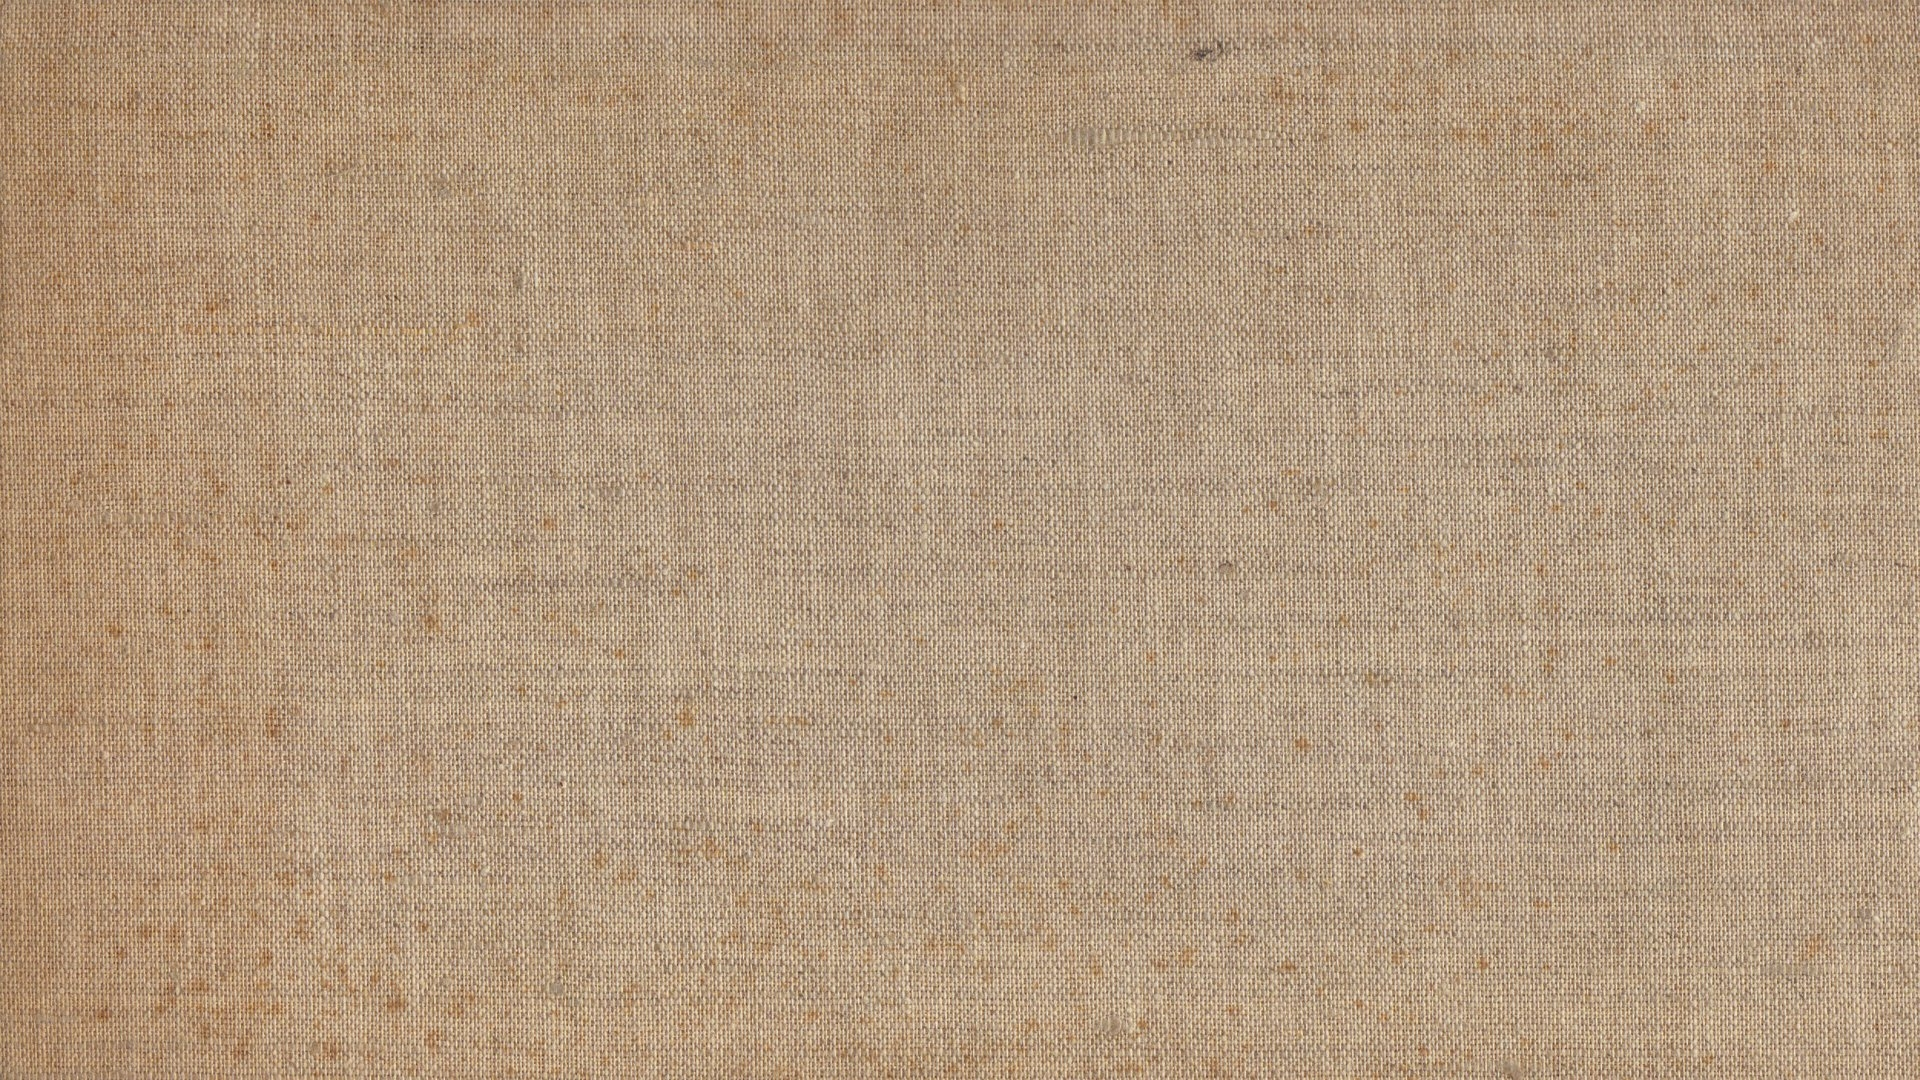
\includegraphics[width=\paperwidth,height=\paperheight]{len}
		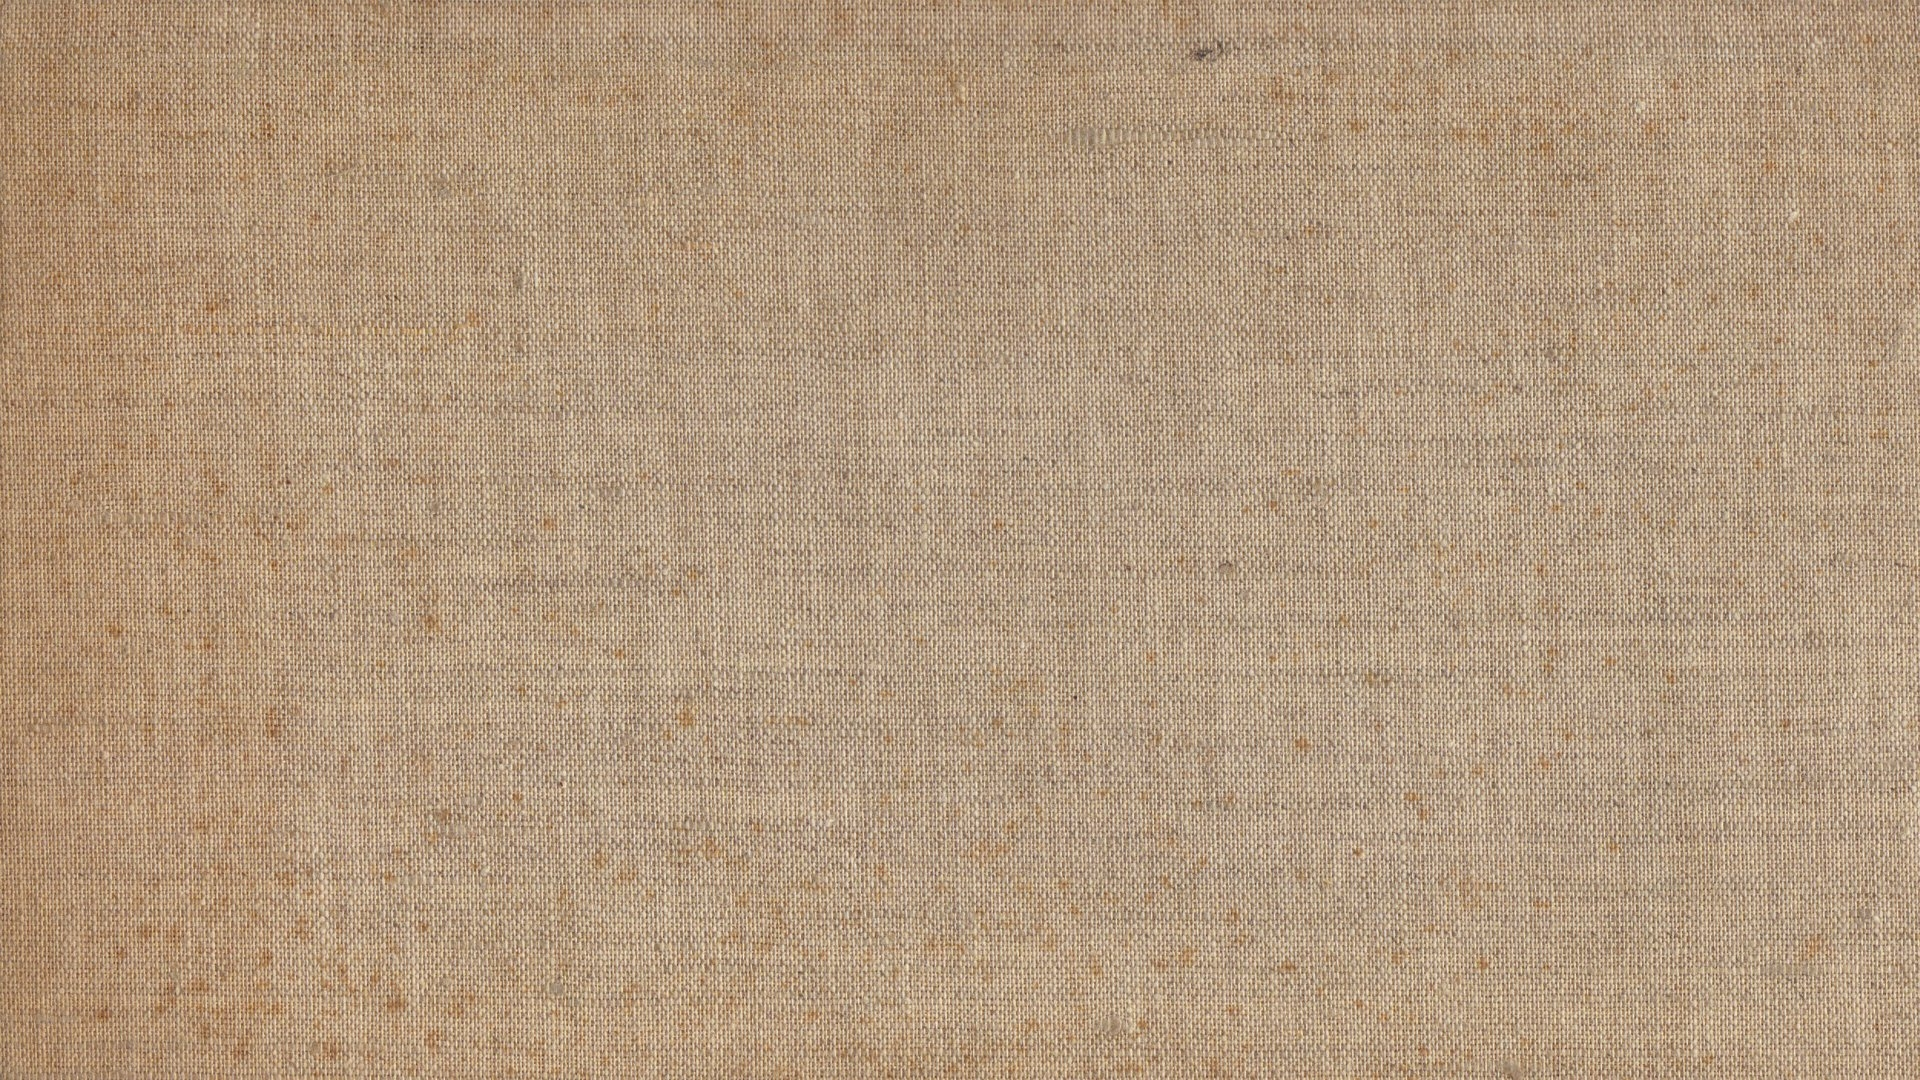
\includegraphics{len}
	}%
}
%%%%%%%%%%%%%%%%%%%%%%%%%%%%%%%%%%%%%
%\def\wordattachment{Приложение}
%
%\def\writeattachmentnonum#1#2#3{
%	\refstepcounter{attachment}
%	\hfill{\MakeUppercase{\wordattachment}}\vspace{-3mm} \\
%	\null\hfill{#1}\vspace{3mm} \\
%	{
%%		\attachmentsize\centering\MakeUppercase{#2}\par
%		\normalsize\centering\MakeUppercase{#2}\par
%	}
%	\addcontentsline{toc}{attachment}{\wordattachment.~#2}
%	\ifx&#3&\else
%	\label{#3}
%	\fi
%}
%%%%%%%%%%%%%%%%%%%%%%%%%%%%%%%%%%%%%%%%%%%%%%%%%%%%%%%%%%%%%%%%%%%%%%%%%%%%%%%%%
%% Вставляет приложение
%% \attachment{description}{title}[label]
%\def\attachment#1#2{
%	\@ifnextchar[
%	{\attachment@i{#1}{#2}}
%	{\attachment@i{#1}{#2}[]}
%}
%
%\def\attachment@i#1#2[#3]{
%	\newpage
%%	\ifnum\getnum{lastattachment}=1
%	\writeattachmentnonum{#1}{#2}{#3}
%%	\else
%%	\writeattachmentnum{#1}{#2}{#3}
%%	\fi
%}
%\usepackage{titlesec}
%\renewcommand{\thesection}{\Asbuk{section}}
%\newcommand{\intro}[1]{
%	\stepcounter{section}
%	\section*{\hfillПРИЛОЖЕНИЕ \arabic{section}}
%	\begin{center}
%		\bf{#1}
%	\end{center}
%%	\markboth{\MakeUppercase{#1}}{}
%%	\addcontentsline{toc}{chapter}{Приложение \arabic{section}. #1}
%}

\renewcommand{\thefootnote}{\fnsymbol{footnote}}
%%%%%%%%%%%%%%%%%%%%%%%%%%%%%%%%%%%%%
\begin{document}
%%%%%%%%%%%%%%%%%%%%%%%%%%%%%%
%
% Координаты стоянок
%
%%%%%%%%%%%%%%%%%%%%%%%%%%%%%%
\newcommand\LidSevenStapel{${N~59.77112\degree~E~34.87456\degree}$} % Стапель 2017 г.
\newcommand\LidSevenFirst{${N~59.68915\degree~E~34.89413\degree}$} % 1 стоянка 2017 г.
\newcommand\LidSevenGES{${N~59.68745\degree~E~34.92153\degree}$} % ГЭС 2017 г.

%%%%%%%%%%%%%%%%%%%%%%%%%%%%%%
% р.Лидь

%	${N~59.77112~~E~34.87456}$ & --- & стапель, п.б., 2017~г.\tabularnewline
%	${N~59.68915~~E~34.89413}$ & --- & ночёвка, л.б., 2017~г.~(4)\tabularnewline
%	${N~59.68745~~E~34.92153}$ & --- & разр.~пл., высадка л.б., 2017~г.\tabularnewline
%	${N~59.67229~~E~34.94233}$ & --- & высадка п.б., 2017~г.\tabularnewline
%	${N~59.64044~~E~35.06237}$ & --- & ночёвка, п.б., 2017~г.~(4)\tabularnewline
%	${N~59.53621~~E~35.19714}$ & --- & ночёвка, л.б., 2017~г.~(2)\tabularnewline
%	${N~59.51290~~E~35.21290}$ & --- & стапель, л.б., 2015~г.\tabularnewline
%	${N~59.46437~~E~35.17958}$ & --- & первая стоянка, л.б., 2015~г.~(3)\tabularnewline
%	${N~59.42332~~E~35.15214}$ & --- & днёвка, п.б., 2017~г.~(5-)\tabularnewline
%	${N~59.38460~~E~35.17379}$ & --- & супер-место, л.б.~(5)\tabularnewline
%	${N~59.32765~~E~35.17302}$ & --- & ночёвка, п.б., 2015~г.~(3)\tabularnewline 
%	${N~59.19729~~E~35.17220}$ & --- & ночёвка, п.б., 2017~г.~(3)\tabularnewline
%\end{longtable}
%
%\subsection*{~р.Горюн}
%\begin{longtable}[c]{>{\raggedright}m{40mm} >{\raggedleft}m{7mm}>{\raggedright}p{65mm} }		
%	${N~59.29726~~E~34.92587}$ & --- & стапель, л.б., 2016~г.\tabularnewline
%	${N~59.27053~~E~34.91910}$ & --- & разр.~пл., высадка л.б., 2016~г.\tabularnewline
%	${N~59.21645~~E~34.92776}$ & --- & высадка на мысу, л.б., 2016~г.\tabularnewline
%\end{longtable}
%
%\subsection*{~р.Чагода}
%\begin{longtable}[c]{>{\raggedright}m{40mm} >{\raggedleft}m{7mm}>{\raggedright}p{65mm} }		
%	${N~59.29726~~E~34.92587}$ & --- & стапель, л.б., 2016~г.\tabularnewline
%	${N~59.21637~~E~34.94938}$ & --- & ночёвка, л.б., 2016~г.~(4-)\tabularnewline
%	${N~59.21520~~E~34.95573}$ & --- & стоянка, л.б.\tabularnewline
%	${N~59.15709~~E~35.23621}$ & --- & днёвка, л.б., 2015~г.~(4)\tabularnewline
%	${N~59.15804~~E~35.24190}$ & --- & ночёвка, л.б., 2017~г.~(4)\tabularnewline
%\end{longtable}
%
%\newpage 
%\subsection*{~р.Чагодоща}
%\begin{longtable}[c]{>{\raggedright}m{40mm} >{\raggedleft}m{7mm}>{\raggedright}p{65mm} }		
%	${N~59.15379~~E~35.30460}$ & --- & семафор, л.б. \tabularnewline
%	${N~59.15912~~E~35.32931}$ & --- & высадка в магазин, л.б., 2015~г.\tabularnewline
%	${N~59.15858~~E~35.32970}$ & --- & высадка в магазин, п.б., 2016~г., антистапель 2017~г, 2018~г.\tabularnewline
%	${N~59.16139~~E~35.37266}$ & --- & стапель, л.б., 2019~г.\tabularnewline
%	${N~59.13567~~E~35.61832}$ & --- & ночёвка за Мегрино, л.б., 2015, 2016, 2019 гг.~(5)\tabularnewline
%	${N~59.06962~~E~35.86246}$ & --- & ночёвка, л.б., 2019 г.~(4-)\tabularnewline
%	${N~59.08257~~E~35.94123}$ & --- & ночёвка, л.б., 2015~г.~(3)\tabularnewline
%	${N~59.08569~~E~35.94522}$ & --- & ночёвка, л.б., 2016~г.~(4)\tabularnewline
%	${N~59.12318~~E~36.03306}$ & --- & днёвка, л.б., 2019~г.~(5)\tabularnewline
%	${N~59.18169~~E~36.11501}$ & --- & днёвка, л.б., 2015~г.~(5)\tabularnewline
%	${N~59.19177~~E~36.15595}$ & --- & экстр. ночёвка, п.б., 2016~г.~(1)\tabularnewline
%	${N~59.18664~~E~36.22300}$ & --- & высадка, л.б., 2015~г., 2016~г.\tabularnewline
%	${N~59.19248~~E~36.23246}$ & --- & антистапель, л.б., 2015~г.\tabularnewline
%	${N~59.16482~~E~36.28046}$ & --- & днёвка, л.б., 2016~г.~(5)\tabularnewline
%	${N~59.15593~~E~36.32325}$ & --- & ночёвка, л.б., 2019~г.~(3)\tabularnewline
%	${N~59.05216~~E~36.40635}$ & --- & ночёвка, антистапель л.б., 2019~г.~(5)\tabularnewline
%	${N~58.99856~~E~36.52885}$ & --- & ночёвка, л.б., 2016~г.~(3)\tabularnewline
%	${N~58.97235~~E~36.58830}$ & --- & антистапель, л.б., 2016~г.\tabularnewline
%\end{longtable}
%
%\newpage 
%\subsection*{~р.Песь}
%\begin{longtable}[c]{>{\raggedright}m{40mm} >{\raggedleft}m{7mm}>{\raggedright}p{65mm} }
%	${N~58.93065~~E~34.15118}$ & --- & стапель\tabularnewline	
%	${N~58.92815~~E~34.20071}$ & --- & завал без обноса\tabularnewline	
%	${N~58.92943~~E~34.23585}$ & --- & ночёвка, л.б.~(4)\tabularnewline	
%	${N~58.92517~~E~34.27858}$ & --- & завал с обносом, п.б.\tabularnewline	
%	${N~58.89480~~E~34.35690}$ & --- & ночёвка, л.б.~(5)\tabularnewline	
%	${N~58.84678~~E~34.44593}$ & --- & ночёвка, л.б.~(5)\tabularnewline	
%	${N~58.90267~~E~34.60336}$ & --- & днёвка, л.б.~(5)\tabularnewline	
%	${N~58.96410~~E~34.84470}$ & --- & ночёвка, л.б.~(5)\tabularnewline	
%	${N~58.94978~~E~34.87727}$ & --- & завал без обноса\tabularnewline	
%	${N~58.93968~~E~34.88977}$ & --- & завал с обносом, п.б.\tabularnewline	
%	${N~58.96258~~E~35.12499}$ & --- & ночёвка, л.б.~(4)\tabularnewline	
%	${N~59.02471~~E~35.21774}$ & --- & ночёвка, п.б.~(4-)\tabularnewline	
%\end{longtable}	

\relpenalty=10000
\binoppenalty=10000
\clubpenalty=10000  % Это костыль против
\widowpenalty=10000 % "висячих" строк
\righthyphenmin=200 % Избавляемся
{\sloppy	        % от переносов слов
%\BgThispage % Фон
\begin{titlepage}
	\newpage
	\begin{center}
		\Large \textbf \MyVarAuthorName
	\end{center}	
	\vspace{1.75cm}	
	%
	%\greenline
%	\uzor
	\begin{center}
	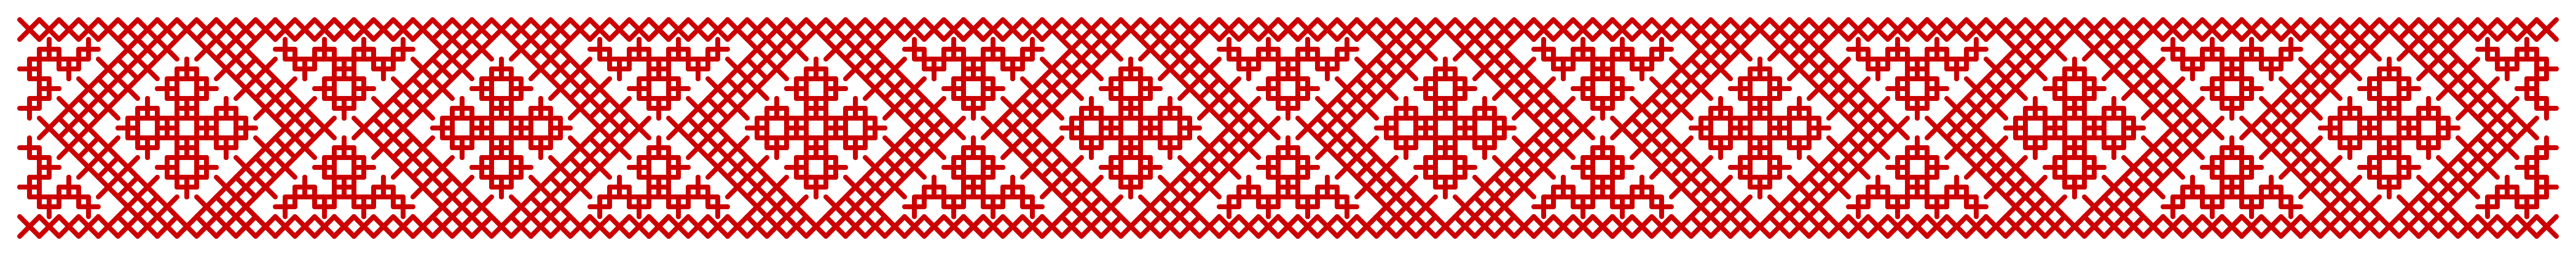
\includegraphics[scale=0.08]{veps}
	\end{center}	
	%
	\begin{center}
		\Huge{\addfontfeature{LetterSpace=32.0}{ВЕПССКАЯ\\ЛЕТОПИСЬ}}
	\end{center}	
%
%	\greenline
%	\uzor
	\begin{center}
	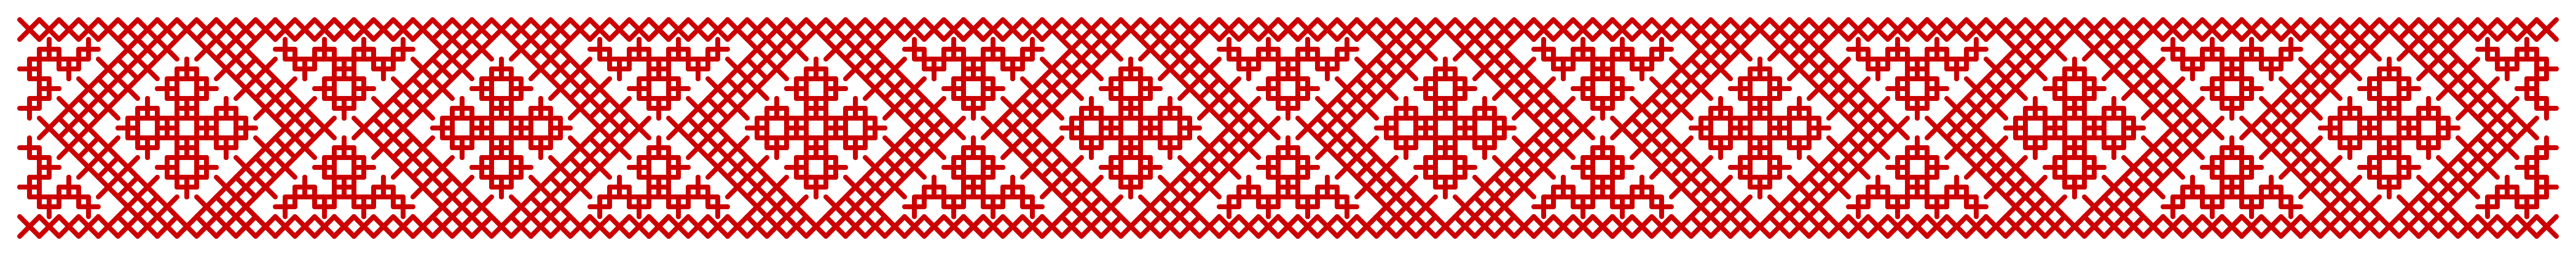
\includegraphics[scale=0.08]{veps}
	\end{center}
%
	\begin{center}
		\footnotesize
%		\small 
%		\normalsize
%		{\addfontfeature{LetterSpace=12.0}
%		СБОРНИК ПОВЕСТЕЙ О СПЛАВАХ НА БАЙДАРКЕ}
%	
%		{\addfontfeature{LetterSpace=2.4}
%		ПО~РЕКАМ ГОРЮН, ЛИДЬ, ЧАГОДА, ЧАГОДОЩА, ПЕСЬ}		
		{\addfontfeature{LetterSpace=10.5}
		\textbf{СБОРНИК ПОВЕСТЕЙ О СПЛАВАХ НА БАЙДАРКЕ}}
		
		{\addfontfeature{LetterSpace=0.1}
		\textbf{ПО~РЕКАМ ГОРЮН, ЛИДЬ, ЧАГОДА, ЧАГОДОЩА, ПЕСЬ}}		
	\end{center}
%
%	\greenline
%	\uzor
%	\begin{center}
%	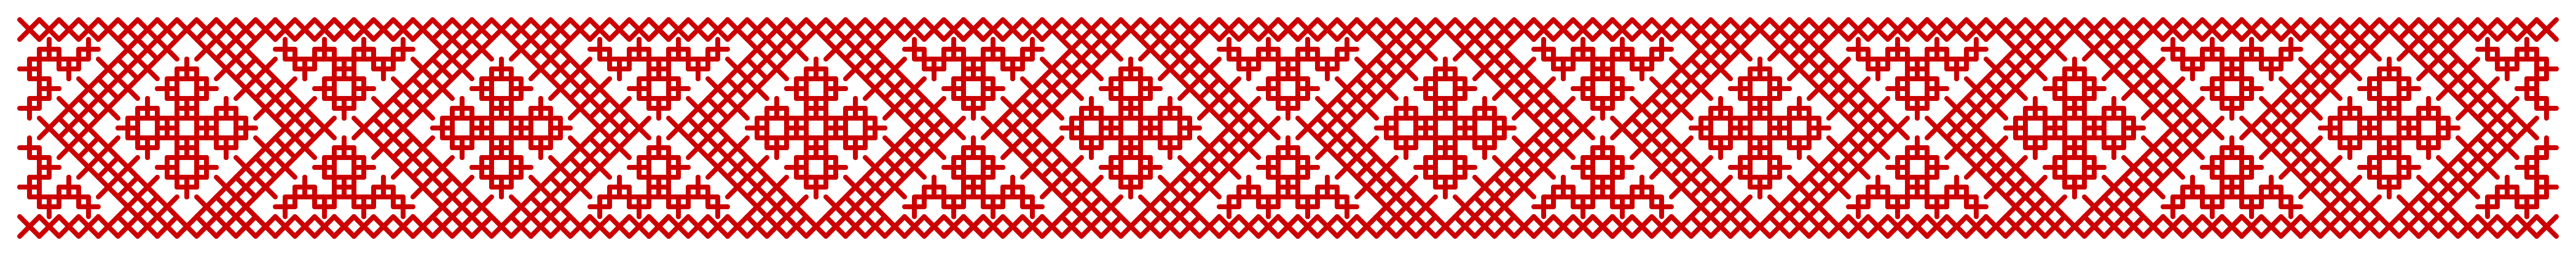
\includegraphics[scale=0.08]{veps}
%	\end{center}
	%	
%	\vspace{\fill}	
%	\begin{center}
%		\small\textbf{
%		Москва \linebreak 
%		2022 \linebreak
%		Самиздат}
%	\end{center}
	\vspace{\fill}	
	\begin{center}\normalsize Москва\end{center}
	\vspace{-1.1cm}
	\begin{center}
\includegraphics[scale=0.12]{maska}\end{center}
	\vspace{-1.24cm}
	\begin{center}\normalsize 2022\end{center}	
\end{titlepage}   % Обложка
%\chapter*{}
%\newpage
{
\thispagestyle{empty}
%
\small{
\begin{flushleft}
\textbf{%
	УДК \UDK \\
	ББК \BBK \\
	\BibCode \\
}
\end{flushleft}
%
\vspace{3cm}
%
\begin{flushright}
{
\begin{tabular}[c]{>{\raggedright}m{14mm} >{\raggedright}m{95mm} }
	\textbf{\BibCode} & \MyVarAuthorName \tabularnewline
	~ & \MyVarBookName \tabularnewline
	~ & \MyVarBookNamesec \tabularnewline
	~ & М.:~ООО~<<ИПЦ~"`Маска"'>> ,~2023\mdash \pageref{LastPage} c. \tabularnewline
	~ & \textbf{\ISBN}
\end{tabular}
}
\end{flushright}
%
\vspace{4.0cm}
%
\begin{flushright}
\textbf{%
	УДК \UDK \\
	ББК \BBK \\
	\BibCode \\
}
\end{flushright}
%
%\vspace{\fill}
\vspace{1.0cm}
%
}
{
\begin{longtable}[c]{>{\raggedright}m{55mm} >{\raggedleft}m{55mm} }
	\textbf{\ISBN} & {\copyright~\MyVarAuthorName,~2023} \tabularnewline
\end{longtable}
}
}
\chapter*{}

В сборник вошли повести по байдарочным сплавам за период с 2015 по 2019 годы. Каждая повесть представляет собой рассказ отчёт по одному из водных походов, проходивших на реках Чагодощенского края и оставивших неизгладимые впечатления в душе автора. В каждой части переплетены воедино сведения о подготовке к сплаву, о маршруте и его прохождении, а также личные переживания автора и множество сопутствующих отвлечённых рассуждений вместе с элементами автобиографии.

\vspace{\fill}
\begin{flushright}
	\copyright~Соболев~А.А.~2022
\end{flushright}
 % Аннотация глобально к сборнику
%\afterpage{\blankpage}
%\tableofcontents
% Замена \blankpage в данном случае:
\newpage
\null
\thispagestyle{empty}
\newpage
%
{
%\setlength{\cftbeforetoctitleskip}{1.5cm}%чтобы влезло на 1 страницу 11 шрифт
%\setlength{\cftbeforetoctitleskip}{0.5cm}%чтобы влезло на 1 страницу 12 шрифт
\setlength{\cftbeforetoctitleskip}{0cm}%чтобы влезло на 1 страницу 12 шрифт c прологом
\tableofcontents
}
%\afterpage{\blankpage}
%\afterpage{\blankpage}
%
% БЛАГОДАРНОСТИ 
\cleardoublepage
\phantomsection
\thispagestyle{empty}
\addtocontents{toc}{\vspace{-10mm}}
\addcontentsline{toc}{chapter}{Благодарности}
\section*{Благодарности}
\begin{enumerate}
\itemsep0.1mm 
%\item[\ding{72}] Моим родителям\mdash без комментариев.
%
\item[\ding{72}] Моей любящей жене Екатерине, которая стала первопричиной моего увлечения водным туризмом и~идеальной спутницей не только в походах, но~и~в~жизни.
%
\item[\ding{72}] Красавину\enskip Сергею\enskip Юрьевичу\mdash моему наставнику, коллеге и~товарищу, за многолетнюю совместную работу, за поддержку, бесценные советы и~опыт, за~знакомство с миром байдарочной свободы.
%
\item[\ding{72}] Краузу\enskip Павлу\enskip Викторовичу\mdash моему коллеге и~товарищу, за ежегодное участие в наших авантюрах, абсолютную стойкость в перенесении походных условий и отличную рыбалку.
%
\item[\ding{72}] Лунёву\enskip Сергею\enskip Александровичу\mdash моему другу и~товарищу, одногруппнику по институту, за~многолетнюю дружбу и за то, что ты преодолел тогда боязнь воды.
%
\item[\ding{72}] Рябкову\enskip Кириллу\enskip Александровичу\mdash моему другу и~товарищу, за неоценимый вклад в психологический баланс в нашей группе; очень жалею, что раньше не~узнал о том, что ты тоже байдарочник!
%
\item[\ding{72}] Горшкову\enskip Александру\enskip Геннадьевичу\mdash моему~другу и~товарищу, однопоточнику по институту, за~неоценимый вклад в атмосферность путешествия и~игру на~губной гармошке.
%
\item[\ding{72}] Голованову\enskip Олегу\enskip Юрьевичу\mdash моему~другу за~характер спокойно\sdash размеренный, за шикарную рыбалку, мелодично\sdash красивую игру на гитаре у костра, стоическое перенесение погодных условий.
\end{enumerate}
\afterpage{\blankpage}
%
% ПРОЛОГ
\newpage
{
\addtocontents{toc}{\vspace{-4mm}}
\addcontentsline{toc}{chapter}{Пролог}
\addtocontents{toc}{\vspace{-2mm}}
\thispagestyle{empty}
\section*{Пролог}

Текст
}

\afterpage{\blankpage}
%
\chapter*{}
\begin{flushright}
\vspace{2.0cm}
\textit{ \large {
Жаждущим диких походов посвящается.\\
\vspace{\fill}
Все имена, названия, события,\\
время и место действия вымышлены,\\
а совпадения случайны.
}}
\end{flushright}



%\afterpage{\blankpage}
%
% ЧАСТЬ 1 - ЛИДЬ 2015
%
\part{Лидь-Чагода-Чагодоща 2015}
\chapter*{}
В повести рассказывается о~первом длительном самостоятельном сплаве автора одной байдаркой по~участку маршрута~№57 \cite{Рыжавский1,Рыжавский2} на~границе Ленинградской и~Вологодской областей. Даётся~развёрнутое описание каждого дня похода с~личными ощущениями и~переживаниями руководителя, оказавшегося на~реке с~двумя малознакомыми матросами. На~долю путешественников выпадают испытания, которые придётся преодолеть вдали от~цивилизации один~на~один с~природой, и~с~этой задачей они успешно справятся. Также~вашему вниманию предлагается предыстория этого похода и~множество отвлечённых рассуждений.
%\vspace{\fill}
%\begin{flushright}
%	\copyright~\MyVarAuthorName,~2022
%\end{flushright}
%\afterpage{\blankpage}
%\chapter*{}
\begin{flushright}
\vspace{2.0cm}
\textit{ \large {
Жаждущим диких походов посвящается.\\
\vspace{\fill}
Все имена, названия, события,\\
время и место действия вымышлены,\\
а совпадения случайны.
}}
\end{flushright}



\afterpage{\blankpage}
\chapter{Несколько слов о сплавах} 
\corner{64}

\vspace{-0.5cm}
\epigraph{%Не нужен бродягам дом и уют \\
%	Нужны - Океан, Земля \\
%	Что звёзды Медведицы им поют \\
%	Не знаем ни ты, ни я \\
%	~...\\
	Вел\'{и}к Океан и Земля велик\'{а},\\
	Надо бы всё пройти,\\
	Большая Медведица издалека \\
	Желает тебе пути.}
	{
	\begin{flushright}
		\small{Станислав~Пожлаков,\\<<Баллада~о~детях~Большой~Медведицы>> из~х/ф~<<Идущие~за~горизонт>>,~1972}%\\(экранизация~повести~Олега~Куваева\\ <<Птица~капитана~Росса>>,~1968)
	\end{flushright}
	}

Неизвестно, от чего получаешь б\'{о}льшее удовольствие\mdash от подготовки к сплаву, от собственно самого сплава или от смакования воспоминаний о нём в кругу друзей, родственников и единомышленников. Каждая часть этого действа хороша по\sdash своему и от каждой остаётся определённый отпечаток, который уже никогда никуда не денется и будет греть душу туриста\sdash водника долгими зимними вечерами.

В широко известной в узких кругах книге <<На~байдарке>> \cite{Квадригин} есть строки о том, что водниками не становятся\mdash в водный туризм втягивают. И это действительно так. Правда, осознаётся это только после нескольких сплавов. Меня втянула в водный туризм тогда ещё будущая жена, предложив сходить в сплав, сама видимо не вполне осознавая, на что идёт. С тех пор в моей душе поселился огонёк странствий по водным просторам нашей необъятной Родины.

Первый сплав\mdash это всегда особенное действо. После него люди либо брезгливо убегают прочь от <<этих ненормальных>> с рюкзаками и вёслами, так и не поняв, зачем всё это надо, либо в их сердцах поселяется огонь странствий, а в мозгу заседает заноза, не дающая покоя ровно от предыдущего сплава до следующего. 

С первым сплавом мне и будущей жене повезло\mdash мы попали на Южный Урал, реку Зил\'{и}м. Сплавлялись около 10 дней, на катамаранах, вместе с огромной компанией в 50 человек, среди которых было 5 или даже больше инструкторов. Река Зилим летом спокойная, но мелковатая в верховьях. Туристы-водники, любящие бурлящую воду и~белую пену, брезгливо называют такие сплавы матрасными. Что ж, это в какой-то мере справедливо\mdash течение реки спокойное, грести особо не надо, лишь местами могут встретиться быстринки и подобия перекатов. Но, в конце концов, все виды отдыха хороши. Мне, жене, да и всем тем людям, с кем мы ходили, нравится именно такой вид сплава\mdash без риска для жизни, но со спокойным единением с необычайно красивой природой нашей страны, когда забываешь обо всех проблемах и заботах, тяготящих тебя в~обычной жизни$\ldots$
\newpage
Инструкторы были заняты на стоянках приготовлением еды на костре, заготовкой дров бензопилами, ну и~конечно травлей анекдотов. Фактически, нам, как новичкам, оставалось только поставить палатку, покидать в неё свои вещи, да наслаждаться жизнью, травить байки и ожидать пока поспеет вкуснейшая вечерняя похлёбка от штатного кока, да закипит чай с душистыми травами, собранными на~местных лугах. 

Нам с будущей женой всё было в новинку\mdash мы никогда не ходили в походы или сплавы. И хотя я много раз порывался выбраться в какой-нибудь поход, каждый раз меня что\sdash то останавливало. Причём перспектива походной жизни меня никогда не страшила\mdash наоборот, мне очень хотелось попасть в настоящий поход и приобщиться к дикому туризму, но всё почему-то не получалось. А тут мы удачно попали в большую команду, нам выдали палатку, снаряжение. Словом, мы упростили себе <<порог вхождения>> в дикий туризм тем, что вопросы, связанные с маршрутом, заброской и выброской, снаряжением решали не мы, а руководители.

В первом сплаве мы испытали на себе и каменистые отмели, когда острые камни противно трутся о дно катамарана, и быстрые перекаты, когда река ускоряется в скалах Южного Урала и надо активно подгребать веслом, выправляя курс. Было и жаркое палящее солнце, моментально высушивающее намокшую одежду, и ураганный ветер с дождём, порой настигающим совсем не вовремя\mdash на воде или когда ставишь палатку. Была~и~походная баня. Это изобретение заслуживает отдельного рассказа, а тот, кто её придумал, безусловно, достоин какой-нибудь премии.
\newpage
Баня в походе\mdash это Баня с Большой Буквы. Помыться, в принципе, можно и в реке, но разве это хоть в какой\sdash то мере сравнится с ощущениями от Бани? Распаренный, вдыхая аромат трав, подстеленных на каменистый берег в роли коврика, хлещешь себя берёзовым, дубовым, еловым, пихтовым веником\mdash любым каким смог сделать. Инструктор, который уже тебе товарищ и друг и с которым выпиваешь по чарке за ужином, обсуждая как классно вообще жить на Земле, плещет воды на каменную печь, и по Бане расходится превосходный пар, обдавая тело волнами колкого тепла. Веники ходят по спинам, раскаляя их докрасна$\ldots$~После, Баня открывается и распаренные, будто заново родившиеся, счастливые туристы с визгами восторга бегом мчатся в речку\mdash окунуться с головой, остудиться и~проплыть пару метров, а потом обратно\mdash греться и снова париться. Особого шика добавляет то, что если во время этого действа идёт тёплый летний дождик$\ldots$  

Сама Баня состоит собственно из печки и палатки, которую ставят потом поверх протопленной печи. Печь~складывают из камней, коих имеется неограниченное количество на берегах рек Южного Урала, выбирая при этом такие, чтобы не трескались при нагреве. Как выбирать\mdash эту науку постигли только Инструкторы, ходящие на эти реки как к себе домой по несколько раз каждый год (вернее\mdash эти реки и есть их второй дом$\ldots$). Потом~ставится палатка\mdash вроде торговой, представляющая из себя куб или прямоугольный параллелепипед и сверху накрывается дополнительно полиэтиленовой пленкой, чтобы меньше уходило тепло и пар. Далее кто-нибудь снаряжается за травой или папоротником для банного пола и ветками для веников. Всё, потрясающие ощущения гарантированы!
\newpage
После Бани чистые, обновлённые туристы усаживаются к импровизированному столу вкушать отменный ужин от кока и пить вкуснейший чай с местными травами. Уже начинает темнеть и сытые, чистые, счастливые люди разбредаются кто куда\mdash часть попеть у костра, часть медитировать на берег реки, кто-то подальше от костра и людей смотреть или фотографировать звёзды, а кто по палаткам творить походную романтику. Уверен, что походная романтика создала немало счастливых семей, где Она знает, что Он может добыть дров, развести огонь и~вообще, что топор из рук не валится. Он, в свою очередь, знает, что Она может фактически из ничего приготовить вкуснятину к ужину и уж конечно оба они\mdash туристы\sdash водники, всегда готовые прийти на помощь друг другу и~поделиться последним, неважно, куском хлеба или сухим спальником. 

Стапель на Зилиме был в Толп\'{а}рово, а снимались с~маршрута в Именд\'{я}шево. Толпарово\mdash прекрасное место! Мост через реку, поросшие соснами склоны горы Карамал\'{ы}, сельские домики, сельхозтехника, огороженные пастбища, стога сена$\ldots$~Я смотрел на всю эту красоту и не мог поверить, что всё происходящее\mdash реальность. Мне казалось это какой\sdash то параллельный мир. Какая\sdash то вдруг Швейцария, внезапно. Но нет, это наша страна, это Южный Урал! Всё\sdash таки как велика, необъятна, красива наша Родина!

На маршруте мы побывали около небольшого интересного озера недалеко от берега реки. Вода в нём была прозрачной, небесно\sdash голубого цвета, и очень\sdash очень холодной. Погода в тот момент была прохладной и дождливой, но всё равно среди нашей команды нашлись смельчаки, окунувшиеся в это природное чудо. Потом мы побывали в~пещере Победа, для чего потребовалось карабкаться вверх в горы по крутым склонам\mdash вход в пещеру находился высоко наверху. Всё это, конечно же, оставило неизгладимые впечатления в наших сердцах! Попасть в такое приключение было настоящей удачей.

Так я изложил общие впечатления человека, втянутого по собственной воле в туристическое братство и в первом же сплаве произнёсшего страшную клятву туристов-водников. После первого сплава был и второй\mdash по Башкирской реке Белая (Агид\'{е}ль) компанией из 10 человек. Этот,~более камерный что ли, сплав на катамаранах также нам очень понравился. В перерыве между первым и вторым сплавом моя женщина, спутница\sdash красавица, окончательно и бесповоротно стала моей спутницей жизни, что ещё раз подтверждает вышесказанное про походную романтику. Так~что второй раз на воду мы встали уже будучи супругами.

Сплав по Белой, безусловно, отличался от~предыдущего\mdash хотя бы впятеро меньшим количеством народа. У нас также были переходы и днёвки, походные Бани и созерцание звёзд, дегустация мёда и медовухи с~местной пасеки, рыбалка и фотоохота. Ещё было посещение пещеры Сказка, расположенной на живописнейшем склоне горы около Акбул\'{а}тово, и К\'{а}повой пещеры (пещера Шульг\'{а}н\sdash Таш), в которой раньше жили доисторические люди. Впечатлений также хватало, мы набирались опыта\mdash благо есть у кого\mdash наши руководители на всех реках Южного Урала были как родные.

Эти два сплава заложили, можно сказать, основу будущим моим путешествиям. В них я понял, что даже такой не слишком подготовленный человек, как я, вполне справляется с походным бытом и что никаких особенных премудростей не требуется. Нужно лишь желание и~стремление идти вперед. Из этих сплавов я вынес очень хорошие уроки организации всего этого действа, приобрёл уверенность в силе человека противостоять природе и~непогоде. А~это ли не главное? Где\sdash то в глубине души загорелась мысль, что я, в принципе, мог бы и сам организовать такое мероприятие, как сплав.

\begin{center}
	\psvectorian[scale=0.4]{88} % Красивый вензелёк :)
\end{center}
 
\chapter{Байдарка}
\corner{64}

После второго сплава был большой перерыв. Не удавалось выкроить время, чтобы попасть на Южный Урал, да и, откровенно говоря, хотелось чего-то нового. Правда, пока сам не понимал чего. Потом, вместе с рассказами начальника о байдарочных сплавах, пришло осознание\mdash вот оно, это новое! Это же то, что надо! Байдарка! Отдельное судно! Твоё! Собственное! Никаких инструкторов, всё делать самому! Тебе никто не указ! Ты\mdash бесстрашный рекоплаватель и первооткрыватель! Ты\mdash Капитан корабля! Сердце моё застучало чаще, разум затуманился. 

После того, как туман развеялся, было много разговоров и рассказов начальника о том, что такое байдарочный сплав и с чем его едят. Вместе с разговорами пришло и второе осознание\mdash идём на реку! Рассуждали о том, на какую реку идти, как забрасываться и как сниматься с маршрута\ldots~а кроме того\mdash нужны были байдарки. Мой выбор пал на консервативную «Таймень», поскольку нашлись ещё школьные знакомые-одноклассники, готовые отдать каркас, или как говорят водники, «кости», ну а новую ПВХ оболочку, «шкуру», купить не проблема. Не обошлось без влияния наших разговоров\mdash начальник рассказывал, что места в «Таймени» просто завались и это действительно оказалось так.

Вообще, тут стоит отметить, байдарочный поход в данном случае оказался неизбежен, как крах мирового капитализма. Я~попал на работу в «почтовый ящик», начальник, увлекающийся водным туризмом, сама атмосфера «почтового ящика»\ldots~всё это настолько тонко, что почти непередаваемо людям, которым никогда не пришлось столкнуться с этим. А когда я поделился с начальником рассказами о своих прошлых сплавах, то тут\sdash то, надо полагать, в его голове и сложилась картина вновь замаячившей возможности оказаться в привычной стихии. Постепенно мы оба свыклись с мыслью, что однозначно пойдём на реку.

Время летит быстро\mdash зима, весна, покупка опять\sdash таки консервативной палатки\sdash домика (типа «Памирки»), долгие переговоры о передаче байдарки в мои руки и, наконец, я стал счастливым обладателем костей для «Таймени\sdash3». Лишними трёшечные кости точно не будут\mdash вдруг ещё пойдём втроём? Заполучил кильсон, позволяющий собрать из трёхместной байдарки двухместную, а также обзавёлся ПВХ шкурой для «Таймени\sdash 2», поскольку мы планировали идти двумя двухместными байдарками, набрав ещё двоих людей в матросы. Начальник же приобрел каркасно\sdash надувную байдарку «Гарпун\sdash 2», поскольку старые свои «Таймени» давно продал, да и хотел судно полегче. Теперь у нас было то, что понесёт нас на просторы рек! Моё сознание рисовало бесстрашных первооткрывателей времён Великих Географических открытий!

Ранняя весна. Переправил всё снаряжение постепенно в деревню, провёл модернизацию палатки, сделал оттяжки для неё. Настало время для главного\mdash собрал в первый раз байдарку. Это совершенно непередаваемое ощущение. Ещё каких\sdash то 40 минут назад ЭТО было запаковано в огромный рюкзак, потом лежало на траве в виде свёрнутой шкуры и горы дюралевых трубок, а теперь всё собрано в красавицу\sdash байдарку совершенно нешуточных размеров! От такого творения рук человеческих захватывает дух! Очнуться помогают только возгласы жены о том, как эту тяжесть тащить к реке? Да, весит «Таймень» немало, но это того стоит. Не думаю что по простоте конструкции, комфорту, вместимости, ходкости, красоте в конце концов, какая\sdash либо байдарка может сравниться с «Таймень\sdash 2»\ldots~Ух! 

Снаряжение было собрано к майским праздникам\mdash байдарка, палатка, а остальное есть с прошлых сплавов, надо только достать с чердака и антресолей. Более того, обладая комплектом костей на двушку и трёшку, я получил свободу выбора\mdash собирать, соответственно, двухместную или трёхместную байдарку, что, понятно, неплохо. Параллельно с этими заботами прорабатывался маршрут будущего сплава, велась оценка буквально всех мелочей, читались отчеты в интернете\mdash конкретно по планируемым рекам для сплава, да и по другим тоже. Изучал и просто литературу по туризму, выискивая то, что могло ускользнуть от меня ранее. Шутка ли, ведь предстояло первое в моей жизни большое походное мероприятие, которое я планировал от начала до конца сам и сам брал на себя ответственность за всё происходящее.

Разгар весны, потеплело. 9 мая, 70 лет Великой Победы. В~этот день было решено спустить байдарку на воду и опробовать собственно\mdash а каково это\mdash плыть на байдарке? Понятно, что отличается от катамарана, но всё же\mdash как это? Байдарка была доставлена на берег реки Киржач недалеко от железнодорожной станции Илейкино, собрана и спущена на воду. Место стапеля идеальное\mdash есть подъезд к реке, ровный покатый берег, небольшой песчаный пляжик. Минут 30\sdash 40 сборки и ОНА готова! Впечатления и тот трепет, который охватил меня, когда я в первый раз сел в байдарку на воде\mdash непередаваемы совершенно. И вот\mdash первый гребок, второй, третий\mdash я плыву! Нос байдарки рассекает воду, создавая волну, в кильватере бурлят буруны. Вдвоём с отцом прошли не более километра и вернулись обратно\mdash это была только проба пера. Первая тренировка на воде. Своеобразная прелюдия перед чем\sdash то б\'{о}льшим\ldots
 
Река Киржач по весне очень полноводная и течение весьма и весьма быстрое, но, несмотря на это, мы вдвоём без груза легко шли против течения. Правда, в одном месте при сужении русла течение ускорялось, и надо было пройти противотоком в своеобразное «угольное ушко». Это далось нам только раза с третьего\mdash настолько сильным было течение. Мне, понятное дело, очень понравилось, и я подумал\mdash сюда я ещё обязательно вернусь! 

Лето, прекрасная пора, полным ходом идёт подготовка к основному сплаву\mdash закупается белорусская тушёнка, сухие супы, пишется примерная раскладка продуктов, которые купим уже там, на месте, чтобы не тащить всё из Москвы. К этому времени подготовлены, распечатаны и «подняты» топографические карты\mdash гордость Капитана (поднять карту\mdash выделить что\sdash либо на карте цветом и/или дополнительными условными знаками). Приобретён б/у старенький GPS\sdash навигатор, в него заложен маршрут и путевые точки. Кроме того, приобретены армейские бахилы химической защиты\mdash вместо сапог\mdash дешевле в 10 раз, легче раза в 3 и места в миллион раз меньше занимают, поскольку их можно свернуть рулоном. 

Приходит осознание необходимости пойти перед большим сплавом в сплав выходного дня потренироваться. Несмотря на опыт прошлых двух походов, я всерьез опасаюсь что\sdash то не учесть и забыть при подготовке к большому сплаву, потому что на этот раз я действую самостоятельно. Следует также понимать, что маршрут предстоящего двухнедельного путешествия будет проходить порой по очень глухим местам и помощи, в случае чего, ждать будет неоткуда. Хоть и придаёт уверенности участие в мероприятии моего начальника\mdash опытного байдарочника, всё равно дополнительная тренировка лишней не будет. Жена с радостью соглашается выбраться с байдаркой на природу, и мы собираемся.

Выбор падает на ту же реку Киржач, где был первый спуск на воду. Подкупает близость к деревне, удобство стапеля и антистапеля, полноводность и относительная малолюдность\mdash уже далеко не майские праздники, а середина лета\mdash народу на реке заметно поубавилось. Собираем снаряжение, закупаемся провизией и вот мы на стапеле в Илейкино! Заправски, уже в третий раз, собирая байдарку, с лёгкостью на душе мы пакуемся и отчаливаем. Впереди нас ждали 2 дня единения с природой\ldots

Сплав выходного дня удался, хоть и вымотал нас с непривычки. Повезло с погодой\mdash дожди обошли стороной, выглянуло солнце. На пути встретился один обнос\mdash разрушенная плотина бывшей Финеевской ГЭС и один небольшой слив с перепадом сантиметров 10\sdash 15, добавивший немного экстрима. В остальном\mdash очень спокойный и прекрасный маршрут для неспешного сплава. Байдарка приносит удовольствие, это понятно ещё с первого спуска на воду, а когда идёшь с любимым человеком\mdash это вдвойне приятно.

К этому времени было собрано абсолютно всё для основного, большого 10\sdash дневного сплава\mdash закуплена тушёнка, которую везти из Москвы, байдарка подготовлена и упакована, вещи тщательно отсортированы и погружены в гермомешок, куплены железнодорожные билеты, проработан до мелочей маршрут. Учтены все интересные места, предполагаемые места стоянок, вся доступная картографическая информация изучена досконально и достигнуто состояние полной, не побоюсь этого слова, боевой готовности! Но гораздо  важнее уверенность и психологическая готовность\mdash ведь я уже 2 раза был на воде в байдарке. И ещё 2 раза до этого сплавлялся на катамаране. А это все\sdash таки чего\sdash нибудь, да значит. Немного страшит должность и ответственность капитана корабля, но не мы первые, не мы последние! Огорчает то, что жена в этот раз не может пойти со мной, потому что не удалось совместить наши отпуска. Придется обитать в палатке одному\ldots~но это мы обязательно наверстаем с ней в следующем сплаве. 

Экипажи подобраны. Люди относительно незнакомые, но внушающие доверие. С ними проведён инструктаж и психологическая обработка за рюмкой чая о предстоящих трудностях и тонкостях водного похода. Зелёные, они с головой окунаются в преподнесённую мной атмосферу сплава. Также, по моему решению, наша команда встречается вся вчетвером вечером после работы и мы ещё раз всё обговариваем, поскольку я считаю, что знакомиться на стапеле\mdash не самый лучший вариант.

Как и в любом деле, в деле байдарочных сплавов тоже существуют свои законы. Один из них\mdash «Кто\sdash нибудь из команды не сможет пойти». Так и случается\mdash начальник, наш Адмирал и Идейный Вдохновитель, не может идти с нами в силу непреодолимых причин. Из четырёх человек остаётся трое. По плану было две байдарки\sdash двушки, а теперь чего делать? Спасает положение то, что у меня есть кости для трёшки. Покупается шкура трёшки и третье весло, и мы снова команда\ldots
 
Психологически это удар\mdash остаться без Адмирала за несколько недель до сплава. Теперь тяжесть ответственности целиком и полностью ложится на мои плечи\mdash теперь я и Адмирал сплава и Капитан своей байдарки и Штурман и Лоцман\ldots короче говоря\mdash руководитель похода. Для меня это оказалось полной неожиданностью, поскольку я рассчитывал на то, что у нас будет более опытный и бывалый Адмирал, нежели я. Однако, это обстоятельство не опустило мне руки, а наоборот, мобилизовало все психологические и организаторские ресурсы. Остальная часть команды идёт на реку в первый раз и ещё толком не готова, но полна решимости. Изрекая извечное\mdash «Не дрейфь, прорвёмся!», продолжаем подготовку к нашему мероприятию и мчимся в~неизвестность. 

\begin{center}
	\psvectorian[scale=0.4]{88} % Красивый вензелёк :)
\end{center} 
\chapter{Маршрут и сборы}
\corner{64}

Для начала немного сухого формализма\mdash сплав наш проходил на границе Ленинградской и Вологодской областей по рекам Лидь, Ч\'{а}года, Чагод\'{о}ща бассейна Верхней Волги. Даты\mdash с 3 по 13 августа 2015 года. Стапель 4 числа под железнодорожным мостом через Лидь у станции З\'{а}борье железной дороги Вологда\nobreakdash--Санкт\sdash Петербург. Заброска от Москвы поездом с пересадкой в Череповце. 7 ходовых дней, 2 днёвки. Вынужденный антистапель 12 августа около деревни Загр\'{и}вье (рядом более крупная деревня Дубровка) ввиду невыполнения запланированного маршрута на 50 километров до штатного антистапеля в селе Л\'{е}нтьево Устюженского района Вологодской области.  Байдарка\mdash «Таймень\sdash 3» с ПВХ шкурой. Экипаж\mdash Аня, Лёня (её молодой человек) и я.

Теперь подробнее обо всём в деталях. Почему был выбран такой маршрут? Главный Идеолог мероприятия\mdash мой начальник\mdash искал небольшую камерную речку в районе от Москвы до Санкт\sdash Петербурга с относительно удобными вариантами стапеля и антистапеля. Относительно чего? Относительно наших пониманий об удобстве. Понятно, что можно отслюнявить цветных билетов банка России деревенским, и они на тракторе подбросят до реки, но зачем, когда до неё от станции 300 метров? Кроме того, он ранее уже ходил в этом районе в сплавы на реки Песь, Каб\'{о}жа, Мол\'{о}га и проникся какой\sdash то особенной теплотой к этому региону из\sdash за его заброшенности и первозданности.

Не скрою, был изначальный план попасть на реку Чагодощу. Эта идея была поддержана и развита. Рассуждали далее\mdash как попасть туда? С реки Песь? Она скорее всего мелеет к августу и, судя по отчетам в интернете, на ней имеются многолетние завалы, а кроме того с постепенным исчезновением движения поездов по Савёловской железнодорожной ветке, попасть на станцию Хвойная, близ которой протекает эта самая Песь, становится всё сложнее. Все найденные нами варианты заброски на Песь требовали пересадки на автобус, скажем, в Великом Новгороде или того хуже\mdash заброски поездом через Санкт-Петербург. Все эти факторы привели к выбору другого притока Чагодощи\mdash реки Чагоды, в которую, в свою очередь, впадает Лидь. Река Лидь и стала нашим отправным пунктом, а удобный стапель в трёхстах метрах от железнодорожной станции Заборье подкупил нас окончательно. 

Судя по найденным отчетам, Лидь обещала быть красивой и именно камерной речкой, чего так жаждали наши души. Таким образом, маршрут был определён\mdash начать с реки Лидь у станции Заборье, далее попасть в Чагоду, потом Чагодощу, дозаправиться продуктами в городе Чагода, что примерно на 1/3 маршрута и далее до Лентьево с экстренным сходом с маршрута в районе Дубровки (эх, знать бы заранее, что именно так и придётся делать\ldots).
 
Чагода и Чагодоща, напротив, уже не такие камерные реки, как Лидь, но зато более полноводные и достаточно широкие\mdash около города Чагода река достигает примерно 50 метров в ширину, а далее местами и все 100. Из отчётов и спутниковых снимков стал понятен примерный облик рек\mdash узкая в верховьях Лидь, в низовьях течёт в высоких берегах с густым лесом, грунты в основном песчаные, берега имеют песчаные обрывы, порой достаточно большой высоты\mdash около 5\sdash 8 метров. По Чагоде нам необходимо было пройти лишь небольшой участок\mdash характер реки тут обычный, не слишком примечательный\mdash полноводная река с частыми островками ближе к устью. Чагодоща же имеет свой характер\mdash расширяясь примерно с середины маршрута, берега её приобретают такой характер\mdash один обрывистый с сосновым лесом, а второй покатый с песчаным пляжиком и кустарниковой растительностью. Далее за поворотом берега меняются местами и теперь высокий песчаный обрыв оказывается с другой стороны, а отмель располагается напротив\mdash так называемое меандрирование реки на языке гидрологов. На конец маршрута по Чагодоще предполагалось прохождение трёх порогов\mdash Горынь, Буг и Вяльская Гряда. В отчетах было сказано, что это скорее лёгкие шиверы и каких либо опасений не вызывают. 

Что ж, про реки всё стало более менее понятно, однако тень сомнения закралась в душу\mdash мало, очень мало отчетов про Лидь и фотографий оттуда! Неужели так мало людей ходит на неё? Неужели все променяли свои «Таймени» на цветные фантики и продались капиталистам на всякие турции и египты? Почти все найденные отчеты относились к весенним сплавам, а чего ждать от верховьев Лиди в августе? Может там впору пешком по руслу идти, а мы на байдарке хотим. Хоть похожий маршрут и имеется в книге небезызвестного Рыжавского Г.Я. «Бассейн верхней Волги» М.:«Физкультура и спорт» 1981 г. под номером 57, но с 81\sdash го года с окончательным упадком Тихвинской водной системы всё могло очень сильно поменяться. Много, много вопросов оставалось без ответа, но, как говорится, кто не рискует\ldots~маршрут был утверждён окончательным и бесповоротным решением.

Как только маршрут окончательно сложился в умах страждущих приключений, началась подготовка картографического материала. Были раздобыты старые генштабовские карты, распланирован примерный километраж по дням\mdash в какой день сколько необходимо проходить, подобраны примерные места стоянок и тому подобные вещи. В GPS\sdash навигатор были загружены путевые точки, составлена раскладка, куплены железнодорожные билеты на всю команду\ldots~в один конец. На каком\sdash то подсознательном уровне мы решили подстраховаться и не брать обратные билеты заранее, поскольку не были уверены не только в правильности расчета километража по дням, поскольку я делал это впервые в жизни, но и в том, что на маршруте всё будет гладко. В голове крутились строчки песни: «Билет в один конец, весна\sdash а\sdash а»\ldots
 
Потом во время пробного сплава выходного дня по реке Киржач был утоплен старенький навигатор и у него отказал экран. Пришлось одолжить на работе новый, более навороченный, но вполне выполняющий свою функцию навигатор. Впредь будем более чутко относиться к нежной буржуйской технике. Оказалось, что новый навигатор показывал географические координаты, чертил на экране пройденный трек, вёл статистику пройденного пути\ldots~но, несмотря на свою навороченность, не имел карты. Вообще никакой! Для того, чтобы иметь возможность привязаться к местности, я распечатал бумажные карты с координатной сеткой UTM (Universal Transverse Mercator), которая показалась мне удобнее формата градусы/минуты/секунды, а в навигаторе, соответственно, включил отображение координат в формате UTM. Вопрос с навигацией и привязкой к местности был решён.

В полной мере осознал всю мудрость решения приобрести хозяйственную тележку, как только попытался поднять рюкзак с «Тайменью\sdash 3», двуручной пилой, складным стульчиком, бахилами химзащиты, надувными сиденьями и двумя флягами 96\sdash го. Вроде~бы по\sdash отдельности немного веса, а вместе\mdash ого\sdash го! А~ещё палатка, гермомешок со спальником и личными вещами. Не отличаясь силой тяжелоатлета, нести такой рюкзак далее пары метров проблематично. Так что тележка очень и очень пригодилась. Хоть~её~трубки и треснули немного, свою задачу она выполнила до конца.

Печальную тоску навевали вещи, сложенные на диване, и детали байдарки, разбросанные по комнате\mdash КАК это всё впихнуть в рюкзак и гермомешок?! Собравшись с мыслями и повыкинув всего не то чтобы ненужного, но без чего могу обойтись, проведя многократную оптимизацию как состава вещей, так и способа, а также очередности их укладки, добился нужного результата\mdash всё помещается. Итого вышло: огромный рюкзак с байдаркой, герма на 60 литров с личными вещами, палатка, маленькая герма для судового журнала, документов и фотоаппарата. Ура, сборы окончены, можно идти!

Оставалось несколько дней томительного ожидания дня отъезда, отпуска и отпускных соответственно. Всё это время я чуть ли не ежечасно созерцал топографический материал и пересматривал снаряжение на предмет поиска чего бы ещё выкинуть. Однако, в конце концов, я пришёл к выводу, что дальше выкидывать что\sdash либо, сокращая объём и массу снаряжения, просто невозможно и на этом успокоился.

\begin{center}
	\psvectorian[scale=0.4]{88} % Красивый вензелёк :)
\end{center} 
%\chapter{Отъезд. 03.08.15}
\chapter{Отъезд}
%\corner{64}
\vepsianrose

И вот, наконец, настал день отъезда. Как я ждал этого момента! Мой первый по-настоящему самостоятельный большой поход. Этим я грезил примерно с 6\sdash го класса, как только начался курс физической географии$\ldots$~и теперь это\mdash реальность! Это~шаг куда\sdash то вперёд, это абсолютно новый опыт в моей жизни\mdash ничего подобного до этого я не совершал\mdash вот так, полностью автономно и в отрыве ото~всего и вся. Я с упоением воображал по топографической карте реку, обрывистые берега, чистейшие сосновые леса и~песчаные пляжи$\ldots$ 

Поезд Москва\thinspace---\thinspace Череповец отходил от Ярославского вокзала в 21:05. Заблаговременно, часа за полтора, как~всегда не рассчитав со временем, я оказался на вокзале. Совершенно официальная парковка у вокзала обошлась в~100 руб/час. Заняли парковочное место и стали ожидать остальную часть команды. Погода в Москве хмурилась, я~кутался в~штормовку и одновременно старался как можно меньше сомневаться в успехе предстоящего мероприятия. Небо~густо заволокло облаками. Перед парковкой угрюмым от~облачности серым цветом расположилась стена Ярославского вокзала$\ldots$

Ярославский вокзал из Трёх Вокзалов занимает в~моём рейтинге 2 строчку\mdash интересная архитектура и~особенная красота, по~сравнению с~другими. Ленинградский по~соседству\mdash первую, естественно, поскольку сразу приковывает взгляд строгостью стиля и классическими формами. Про Казанский, сборище из бесчисленного количества непонятных пристроек, надстроек и подземелий, говорить совсем не приходится.

Время ожидания тянулось медленно. За полчаса до~отправления или~даже раньше подали поезд, и~вскоре вынырнула из метро моя команда. Увидав~издалека их~огроменные рюкзаки, я~чуть не выругался в~голос\mdash ЧТО они везут?! И это же только одежда и палатка$\ldots$~без~продуктов! Не~для них ли я сто раз переписывал и сокращал список вещей?! В первый раз все этим болеют\mdash тащат с собой кучу ненужного: лишние ботинки, резиновые сапоги, лишнюю смену одежды, лишнее ещё\sdash что\sdash нибудь\sdash тяжелое\sdash и\sdash объёмное и прочее\sdash прочее\sdash прочее. Я~хотел уберечь ребят от этого печального опыта, но~не~сумел\mdash видимо каждый, как ни крути, должен набить себе эту шишку сам, увы. В свой первый сплав я тоже набрал кучу ненужного, чего вполне мог бы не брать. И это было учтено в последующие разы. А тут$\ldots$~видимо, придётся с этим смириться, с этими огромными рюкзаками, что ещё поделать?

Билет на байдарку (какая издёвка!) был приобретён заранее, и с посадкой в поезд проблем не возникло. Билеты на экипаж я купил электронные\mdash предъявляешь только паспорт при~посадке и проходишь$\ldots$~XXI век в~действии, с~ума сойти! Отмечу,~что фирменный поезд {Москва\thinspace\nobreakdash---\thinspace Череповец} номер~126Я~<<Шексна>>\mdash \textit{единственный} поезд из Москвы до~Череповца на~2015~год. 
 
В Череповце нас ждёт пересадка на Архангельский поезд, следующий до Санкт\sdash Петербурга под номером 009С. Сходить нам на станции Заборье, как уже неоднократно упоминалось. До~Череповца от~Москвы ехать 8 часов примерно, от Череповца до Заборья около трёх с половиной. Перерыв между поездами 4 часа\mdash за это время как раз надеялись закупиться продуктами. Ехали везде, естественно, плацкартом\mdash плацкарт наше всё, будь ближе к народу! 

Мы подошли к нашему вагону и начали грузиться. Таскали вещи при загрузке мы, конечно, неприлично долго, но внутри вагона довольно быстро раскидали всё по~просторам третьих полок, а упаковку с байдаркой положили вниз под сиденье. Место на 4\sdash го члена экипажа, билет которого пришлось сдать, никто не занял, и мы с радостью его оккупировали, благо со стороны проводницы никаких претензий не было.

Жена безумно волновалась за меня, и расставание с~ней далось особенно тяжело, хотя Адмирал сплава и~не~должен показывать виду. И вот, последние объятия, все расселись по местам, закончена посадка. Поезд неслышно трогается с~места и плавно набирает ход. Все машут руками, а~жена отходит в сторону на платформе, чтобы дольше было видно меня из окна\mdash машу ей рукой в ответ и шлю воздушный поцелуй. Не горюй, милая, я скоро вернусь, а~сейчас Дух~Авантюризма зовёт меня в путь!
\newpage
Платформа вскоре скрылась из виду, и мы продолжили размещаться в вагоне. Этот самый единственный поезд до Череповца, хорошо ещё, что фирменный, оснащённый биотуалетами и прочими благами цивилизации, удобно прибывает\mdash утром. Как раз ночку поспать и уже приедем. В первый раз мне довелось ехать в плацкарте на нижней полке\mdash всегда брал верхние до этого, куда бы ни ехал. Удобно, что сказать. Никто не сшибает головой твои ноги, свисающие в проход со второй полки при росте за 190 сантиметров. Теперь, на нижней полке, мои ноги сшибают ногами, а не головами. Но не сильно и не матерясь. Терпимо. 

Поезд, тем временем, уже выехал из Москвы, и~начались обычные плацкартные разговоры.  Обо всём по чуть\sdash чуть. Плацкарт, как явление, вещь незаменимая и ни с чем не~сравнимая. Если его когда-нибудь отменят\mdash это~повод для новой Великой Октябрьской как минимум, ибо это будет чересчур. Плацкарт\mdash не просто способ максимально дёшево добраться куда бы то ни было, это$\ldots$~своя атмосфера. Это полки, это проход, это титан в~начале вагона, это еда из~дома в~фольге, а~ещё ноги, свисающие в~проход$\ldots$~ну,~словом, вы понимаете. А если не понимаете, срочно проверьте свой паспорт\mdash вы точно гражданин~России? 

Взяли чаю по 30 что ли рублей. Очарование чая в~стакане с~подстаканником и постоянно позвякивающая ложечка$\ldots$~иностранцам не понять\mdash им главное комфорт, выгода, деньги. Тут же иное. 

Долго болтали о разном, шутили. Волнение команды было видно невооружённым глазом, да я и сам, естественно, волновался, но романтика путешествия и жажда неизведанного звала вперёд. И~всё\sdash таки, в какую авантюру мы ввязываемся! Ух!!! Я~был просто горд собой, что решился на такое и сумел, конечно не без поддержки начальника, организовать свой первый по\sdash настоящему дикий сплав. 

Народ вокруг стал укладываться и мы, последовав их примеру, тоже улеглись пытаться заснуть под стук колёс. Места у нас были в купейной части плацкартного вагона\mdash два нижних и одно верхнее. Я расположился внизу, а~Лёня с~Аней на двух полках напротив. Вскоре выключили основное освещение, оставив только приглушённое ночное дежурное. Поезд смиренно отмерял километры ярославской железной дороги стуком колесных пар$\ldots$

Удалось устроиться удобно и я лежал, укутавшись в~простынь, пытаясь заснуть. Но~сон не шёл\mdash я~не~сильно устал за день и вечер, к тому же перекидывался смс\sdash ками с женой, ловя моменты, когда была связь. Жалко,~что~она не идёт со мной в этот раз и безумно грустно от~этого$\ldots$~уж~кто\sdash кто, а она\sdash то идеальный напарник в походе, в чём я не~раз убеждался.
 
Отгоняю от себя вдруг налетевшую тоску мыслью о~том, что~я\mdash Адмирал сплава и двое зелёных матросов, уже храпящие к этому моменту на соседних полках, на реке будут полностью зависеть от меня. Мне, как предводителю, Адмиралу, придётся давать указания, держать всё под контролем, при этом стараясь не~переусердствовать, и~не~забывать самому принимать в нашем действе самое активное участие. Неведомое ранее чувство особенной ответственности подкатывает, но потом я вспоминаю книгу <<Географ глобус пропил>> \cite{ГеографГлобусПропил} (а также недавно вышедшее по~ней кино) и меня отпускает. 

Одновременно возникает странное неизведанное чувство отрешённости от мира\mdash как будто вся привычная жизнь идёт параллельно нам, а мы как бы со стороны, на~обочине~её, в~параллельных мирах; как будто мы\mdash не~мы, а~кто\sdash то другие, в тельняшках и штормовках\mdash сели в поезд и несёмся навстречу неизвестности. Вскоре веки мои тяжелеют, и я проваливаюсь в сон.

\begin{center}
	\psvectorian[scale=0.4]{88} % Красивый вензелёк :)
\end{center}
%\chapter{Заброска. 04.08.15}
\chapter{Заброска}
\corner{64}

Обычно я не высыпаюсь в поезде и с утра поднимаюсь как варёный рак. Но тут на удивление удалось выспаться. Может потому что на нижней полке? Тем временем проехали Вологду. Скоро уже и Череповец. Погодка стоит безоблачная, разгорается утро. Взяли чаю, перекусили, плацкарт понемногу начал оживать. Поезд прибыл в~Череповец точно по расписанию\mdash в 8:29 утра, конечная. Хорошо\mdash не~надо торопиться с высадкой, вытаскивая наши тяжеленные рюкзаки$\ldots$
 
Поезд останавливается, народ быстренько выходит. Мы не спешим, ждём, пока все выйдут и только потом, последними выходим со всеми своими рюкзаками и~баулами. Вокзал в Череповце достаточно красивый, старый, зелёно\sdash белого цвета. Очарование старых железнодорожных станций\mdash это что\sdash то особенное$\ldots$~стою и рассматриваю вокзал. Ребята подтягиваются со своими огроменными рюкзачищами. Сваливаем вещи горой на скамейку и~усаживаемся передохнуть\mdash баулы наши не из лёгких, а скоро ещё прибавится провизия. Как на стапеле всё это понесём до реки? 

Слегка приходим в себя после поезда. Надо идти закупаться продуктами. Аня~остаётся присматривать за~вещами, а~мы с~Лёней собираемся\mdash берём две сумки и~выходим с~вокзала. 

Первоначально я наметил продуктовые магазины с~противоположной стороны, к~северо\sdash востоку от вокзала, но~как попасть туда мы не~поняли\mdash перехода через пути нет, на~путях стоят грузовые поезда, надо идти до автомобильной эстакады, что виднеется вдоль ж/д путей$\ldots$~далековато. Решили искать магазины на стороне вокзала. Спросили у~местных дорогу и пошли через привокзальный сквер на~юго\sdash запад. Сразу за сквером вышли к~продуктовому на~Комсомольской 39. Разгул капитализма\mdash закупились всем, чем только можно\mdash макароны, гречка, рис, чай, сахар, печенье, сухие супы, сгущёнка в банках и пакетах, хлеб, соль, перец, да всего и не упомнишь. Ещё купили мороженое и пошли обратно к вокзалу. Операция по закупке прошла достаточно резво\mdash быстро вернулись, прикупили местную газету <<Речь>>, пару магнитиков с символикой Череповца и пошли к Ане. Она загорала и читала книжку, ожидая нас. Погода выдалась просто отличная\mdash солнышко, немного белых облачков в высоком синем августовском небе, лёгкий северный ветерок. Прохладно~и~не~жарко\mdash просто~замечательно! 

Наш архангельский поезд отправлялся в 12:08, в запасе было ещё пару часов. За это время надо было снова купить билет на байдарку на вторую часть пути, потому что оформить этот билет в Москве не удалось. Девочки в~кассе сначала отправили меня в терминал, мол распечатай там. Обрадовался! Думаю\mdash ничего себе, до чего дошёл прогресс, сейчас через терминал куплю багажный билет на~байдарку! Но не тут\sdash то было\mdash терминал оказался просто терминалом для распечатывания заранее купленных через интернет простых билетов, не багажных. Делать нечего, надо опять в кассу$\ldots$~терпеливо отстоял очередь в 3\sdash ю кассу. Выяснилось, что билеты на багаж оформляются только в~4\sdash й$\ldots$~где, так и раз эдак, я спрашиваю, это написано?! Нигде! Обычная, касса, как и остальные три! Никаких надписей, что только там можно оформить багаж. Прелести общения с системой. Та самая действительность, от которой я сбегаю на реку$\ldots$

Устроил у касс небольшой скандал чисто из~профилактических целей\mdash мне потрепали нервы\mdash получайте и вы, раз вам так лень повесить хоть какие\sdash то информационные листки или объявления, где было бы русским по белому написано как оформляется багаж. Причём мне уже были готовы оформить и~без очереди, и~прямо сейчас, и~даже не в той кассе, но Штирлиц прокололся, ляпнув, что у него поезд только в полдень$\ldots$ и~снова очередь, теперь уже в 4\sdash ую кассу. Передо мной женщина оформляла возврат какого\sdash то бешеного количества билетов\mdash штук эдак 30\mdash пришлось терпеливо ждать, благо времени вагон$\ldots$~а~если бы было впритык? Тогда бы снова скандал и~тэ~дэ и~тэ~пэ$\ldots$~как же в обыденной жизни раздражают такие моменты. Я~стоял в очереди, а~воображение рисовало мне реку$\ldots$~где нет этой окружающей действительности, где~нет правил, нет этих дурацких билетов и прочей требухи, где~не надо никому подчиняться, где можно всю цивилизацию послать на три буквы, где первобытная свобода ждёт$\ldots$~скоро, очень скоро всё это будет у~нас!
\newpage
Оплатив положенные рубли за провоз байдарки, пошёл к ребятам на улицу. Аня всё это время непрерывно курсировала от Лёни, сидящего снаружи у наших вещей на лавочке, ко мне, стоящему в очереди, подбадривая меня разной болтовнёй. Наконец, покончив с формальностями, мы вместе стали ожидать поезд и читать местную газетёнку, где писали, что первые две недели августа обещают быть жаркими в противовес не слишком\sdash то тёплому лету в этом году. Кутаясь в штормовку от ветра, очень хотелось верить в потепление. По вокзалу особо не бродили\mdash будет время потом, на выброске.
 
Поезд Архангельск\thinspace\nobreakdash---\thinspace Санкт\sdash Петербург номер 009С подошёл минут за 20\thinspace\nobreakdash--\thinspace 30 до отправления. Внимательно вслушивались поначалу в объявление по громкой связи, силясь понять, на какой путь прибывает наш поезд. Потом в~итоге определили это визуально, поскольку, кажется, диктор специально говорила так, чтобы никто ничего не~разобрал. Взяли вещи и пошли не спеша. Оказалось, что у нас последний вагон, да ещё последние места, красота! Проедемся в последнем вагоне. Проводницей оказалась молоденькая студентка какого\sdash то железнодорожного училища. Оказалось, их таких проводниц\sdash студенток на практике\mdash весь поезд почти. Малинник, короче$\ldots$~Округлив глаза на~нашу байдарку, она попыталась что\sdash то пролепетать, мол, не имеет права нас с таким грузом пропускать и вообще чего вы тут. Но не тут\sdash то было! Борзо и дерзко сунув под нос ей бумажку, то есть, пардон, не бумажку, а высочайшую квитанцию об оплате бешеной суммы в сто с чем\sdash то рублей на провоз байдарки, мы с победоносным видом стали грузиться в вагон. Велика Россия, а порядку в ней$\ldots$~Проводники и сами не знают своих правил, которые здравому смыслу вообще не поддаются. То ли денег хотят ещё сверху от наглости и жадности, то ли чего$\ldots$
\newpage
В любом случае, мы погрузились в поезд. Родимый плацкарт, да ещё последний вагон\mdash вообще шик, можно сказать! Ехать~нам до Заборья всего ничего. Четвёртое место в купейной части снова пустовало, что~не могло не радовать. Запихнуть байдарку полностью под~сиденье почему\sdash то не получилось\mdash другой поезд, немного другой размер подполочного пространства? Возможно. 

Поезд~не~фирменный, но все достаточно терпимо. Тем более что потерпеть\sdash то 3.5 часика. Нажимаешь ногой на педальку в уборной\mdash привет, рельсы! Здравствуй, XXI век\mdash век, где можно купить билет на такой поезд через интернет. Мы\sdash то,~собственно, привычные, но так ли должно быть в~XXI~веке?

Время ползло улиткой. В Бабаево остановка на полчаса. Большая станция, депо, поворотный круг. Паровоз~на~постаменте. Дети лазают по~паровозу, как~муравьишки. Мы~с~Лёней вышли, походили, погуляли. Сфотографировали паровоз. На~нём была табличка: <<Заводы им.\thinspace Готтвальда, Брно>>, то есть он оказался чешского производства. Скоро, совсем скоро будем в Заборье. Хочется быстрее туда попасть! Звоню родным, говорю, что у нас всё хорошо и пусть не волнуются. Проводница зовёт всех внутрь, отправляемся. До Заборья остаётся совсем капелька.

Пока едем, снимаю на фото и видео убегающие вдаль рельсы через стекло двери последнего вагона. Завораживающее своей бесконечностью зрелище! Насколько же велики и необжиты пространства нашей огромной страны. И как хорошо, что они медленно обживаются и ещё есть места, не испорченные человеческим присутствием. Сейчас мы стремительно несёмся навстречу именно таким закоулкам Ленинградской и Вологодской областей. В край верховых болот, сосновых лесов и петляющих среди них рек с~тёмной торфяной водой и золотыми песчаными берегами$\ldots$

Договариваемся с проводницей, не зная по наивности, что это вообще\sdash то её обязанность, чтобы она выставила красный флажок, если мы будем не успевать выгрузиться\mdash ведь в Заборье поезд стоит всего одну минуту. Та,~поломавшись для виду, соглашается, кокетливо выясняя о нашем сплаве. 

Народ, проходя мимо нашей байдарки к титану за~кипятком, воняя лапшой быстрого приготовления, косится на наши вещи и лица.  <<Ненормальные>>,\mdash читается в их глазах. Ах\sdash ха\sdash ха! Да, сейчас мы\mdash ненормальные. Мы~несёмся вперед, на просторы. Нас ждёт освобождение от~города, от~цивилизации, от~самих~себя.

И вот, Заборье! Заблаговременно вытащили с Лёней рюкзак с байдаркой в тамбур, сбоку приставили остальные вещи. Стоим в тамбуре, а Аня пока подтаскивает остальные нетяжелые сумки. Как успеть десантироваться за 1 минуту?! Загружались мы обыкновенно минут пять, а выгружались в Череповце из первого поезда ещё дольше, как мне показалось. Волнительно! Наконец~поезд замедляет ход и~останавливается. Проводница открывает дверь и~опускает подножку\mdash момент истины настал! Я мигом вылетаю на~низкую платформу, принимаю у Лёни рюкзак с~байдаркой на тележке, остальные тюки. Парень, который ехал на~боковушке рядом с~нами, помогает подавать вещи$\ldots$

15 секунд. Именно столько, как мне показалось, мы выгружались. Даже возможно меньше. Пока горит спичка, не~иначе. В \cite{Квадригин} также говорится об этом эффекте высадки. Как бы там ни было, все вещи действительно оказались на платформе в мгновенье~ока. Пока я доставал фотоаппарат, чтобы запечатлеть нас и окрестности, поезд снова начал набирать ход. Проводница укоризненно покачала нам на прощание головой, не понимая наших душевных порывов отказаться от всех благ цивилизации, и укатила дальше. Мы~остались одни. В~глуши. Посреди платформы в~неведомых краях на границе Вологодской и~Ленинградской областей. На~стыке двух миров\mdash обыденности и~ярких красок. <<Жребий брошен>>,\mdash мелькнуло у~меня в~голове. Это~было то, чего~я хотел ровно с окончания сплава по~Белой\mdash я~снова на~реке! С~этого момента пути назад нет, только~вперёд, только по~красавице~Лиди!

Платформа в Заборье низкая, асфальт обновляли наверно ещё при советской власти. Зато название станции на табличке сделано в новом серо\sdash красном стиле и на двух языках\mdash продублировано но английском: <<Zaborye>>. Лучше бы поезда обновили, но проще же таблички\mdash как всегда показушничество! 

Ехать в последнем вагоне было хорошо, но дальше идти к реке. Ничего, справимся, куда денемся. Я на мощнейшем эмоциональном подъёме! Сейчас я\mdash первопроходец, разведчик; надо найти подход к реке.  Взваливаю гермомешок с вещами на плечи, рюкзак с байдаркой везу на тележке впереди себя\mdash так мне показалось удобнее. Лёня помогает Ане надеть на спину рюкзачище, а потом и сам взваливает на спину свой тяжеленный 120\sdash литровый рюкзак и берёт две сумки с продуктами. Идём~вперёд, народу никого. Никто кроме нас не сошёл тут с поезда. Идём сначала вдоль станции, а потом по грунтовке метров триста. И~вот\mdash железнодорожный мост через Лидь, а рядом с ним отличное место для стапеля на низком левом берегу. 
\newpage
Сразу оцениваю реку. Мелкая. Дно каменистое, очень отдалённо напоминает берега Зилима, только все сплошь заросшие. Начинаем собирать байдарку. Рядом деревенская ребятня жжёт костер и купается в речке. Спрашиваю про клещей\mdash говорят редкость. Успокаиваемся, продолжаем сборы. Меня, тем не менее, какая\sdash то букашка больно кусает в бок, но вроде не клещ. Немедленно проводим химобработку верхней одежды$\ldots$

По железнодорожному мосту с оглушительным грохотом часто проходят грузовые составы. Вскоре наша байдарка почти собрана. Никак не хочет натягиваться фальшборт. Просто ну никак. Бьёмся с ним очень долго. Наконец, при помощи пассатижей и какой\sdash то матери, удаётся застегнуть последний замок среднего фальшборта. Всё\mdash теперь байдарка готова! Можно грузиться! 

Корабль наш уже спущен на воду, а мы с Лёней в~бахилах химзащиты, шлёпая по воде, таскаем и грузим вещи. Бригада моя распаковывает свои рюкзачищи, в них всё оказывается разложенным по гермомешочкам. Неплохо, учитывая то, что вещи надо распихивать под борта байдарки. Грузовой отсек занимает гермомешок с продуктами, палатки, ещё одна сумка с продуктами и всё остальное по мелочи. Места впритык. При этом моих личных вещей\mdash одна герма, на которой я сижу, да палатка. Мой девиз этого сплава\mdash <<Спарта!>>\mdash у меня с собой даже футболка одна$\ldots$~рюкзаки же ребят фактически некуда девать. Делать нечего, кладу их сверху в~грузовой отсек, накрываю полиэтиленовой плёнкой от дождя, перехватываю крест\sdash накрест резиновыми жгутами. Жить можно. 

Собирались мы неприлично долго. Я планировал встать на воду максимум в половину пятого. Какой~там$\ldots$~стартуем только в 6 вечера. Понимаю, что в любом случае должны пройти запланированные 7\thinspace\nobreakdash--\thinspace 8 километров, чтобы не выбиться из графика, иначе все мои прикидки по километражу собьются, да и заночевать лучше не в населённом пункте, понятно. Координаты стапеля\mdash \CoordsLidFifteenStapel. 

Отчаливаем, садимся, устраиваемся поудобнее. Готово! Я~отталкиваюсь от берега ногой и тоже занимаю капитанское место на корме. Сплав начинается! Время около 18:00. Стапель в Заборье пройден. Впереди нас ждёт свобода, ждут приключения, ждёт полный отрыв\mdash нас ждут 200 километров рек Лидь, Чагода, Чагодоща. 

Речка неширокая, местами очень мелко, течение у стапеля слабое, 1\thinspace\nobreakdash--\thinspace 2~км/ч. Включаю GPS\sdash навигатор, позаимствованный на работе. Оцениваю нашу скорость. Идём хорошо\mdash около 7\thinspace\nobreakdash--\thinspace 8~км/ч. Встречаются каменистые шиверы, но вроде бы идём без повреждений, хотя изредка и цепляем днищем на мелководье. Вода~под ногами\mdash это стекает с бахил химзащиты, когда залезаешь в байдарку, успокаиваю я себя. Мелкие участки заканчиваются вскоре после Заборья, и воды становится заметно больше\mdash хорошо! Я просто упиваюсь восторгом от происходящего\mdash мы на~реке! Мы выбрались из города, мы преодолели себя, свою неуверенность, свои страхи и теперь ничто не отделяет нас от~природы, которая примет нас, смоет с нас городскую грязь, обновит и придаст сил жить дальше$\ldots$

Управлять байдаркой\sdash трёшкой нам с Лёней не особо легко. Также, видимо при загрузке на стапеле я неравномерно распределил вещи и нас кренит влево, отчего мы постоянно поворачиваем. Это приходится исправлять усиленной греблей, потому как руль на байдарке\mdash вещь бесполезная. Аня~же счастливо фотографирует окрестности и привыкает к новой обстановке. 
\newpage
После двух часов сплава, около 20:00, мы~приближаемся к капитальнейшему завалу, позади которого виднеется вышка\sdash засидка. При подходе становится ясно, что справа есть широкий проход и там можно пройти  без проблем. Сразу за завалом резкий поворот влево и мигом вправо открывается вид на автомобильный мост через реку близ Гришкино\mdash ориентир на сегодняшний день, означающий, что километраж прошли. Что~ж, пора искать стоянку! Сразу за мостом, метрах в трёхстах, на левом берегу замечаю приличную полянку, около которой мы и~причаливаем. Дрова есть, место хорошее, хоть и близко к деревне. Скорая разведка показывает наличие проезда к стоянке. Но на сегодняшний день другой альтернативы, судя по карте и времени, у нас нет. Мы разгружаем байдарку и начинаем разбивать лагерь. Координаты первой ночёвки\mdash \CoordsLidFifteenGrishkino. 

Задача сейчас быстро поставить палатки, найти дров, развести огонь и приготовить ужин. А уже вечереет\mdash надо поторапливаться. Мудро взятая с собой по совету начальника двуручная пила творит чудеса, моментально распиливая даже толстые брёвна. Никакие ножовки не идут в~сравнение! Достаю~оргстекло и, используя его как растопку, развожу костёр. Ребята, тем временем, ставят палатку, располагаются. Недолго~совещаясь, на ужин готовим суп и~макароны с тушёнкой. Пока Лёня налаживает нехитрый быт, а Аня готовит ужин, я быстро ставлю свою палатку. Вскоре в результате совместных усилий у нас уже есть ужин, который немедленно и жадно поглощается. Устали. Вымотал~нас не переход, а стапель. Борт~байдарки, который никак не хотел натягиваться, да долгая погрузка. Плюс, конечно, сказывается ночь в поезде и дорога в целом. Но~рядом течёт река, а значит всё хорошо, значит ты\mdash там, где хотел оказаться. Ты\mdash на реке. 
\newpage
Первая стоянка\mdash всегда особенная. Это переход от~городской жизни к~походной. Да\sdash да, именно на~первой стоянке. Не на заброске, не на стапеле, не на первом переходе, а~именно на~первой стоянке. Первая стоянка, как своеобразный итог, результат заброски на маршрут, подводит черту под твоими переживаниями, тревогами и способна окончательно очистить тебя перед Священнодейством Сплава, способна смести в сторону надуманные барьеры, ненужные запреты повседневной городской жизни. Одним словом, после первой стоянки\mdash ты окончательно в \textit{сплаве}, в другой жизни, в другой вселенной, в другом состоянии души. Ты\mdash на реке. И река наша, Лидь, после мелкого участка в Заборье, радует полноводностью.

У костра развожу 96\sdash й в подкотельнике десантного котелка. Набиваю самодельную трубочку из корня винограда ирландским табачком, дымлю не торопясь. Красота! Лёня разливает$\ldots$~отдых начался! Закатное солнце необычайно красиво освещает верхушки сосен на нашем и противоположном берегу. Редкие машины проезжают по мосту неподалёку, нарушая идеальную, просто звенящую в ушах тишину. Птицы изредка подают голоса. Потрескивают сырые дрова в огне. Ветра нет, дым нашего костра поднимается почти вертикально\mdash хороший знак\mdash завтра должна быть хорошая погода. Сверху резко спускается звёздная августовская ночь. Мы лежим у~костра на ковриках и медитируем в оглушительной тишине тихвинских лесов$\ldots$~фантастика! И вроде просто\sdash то как всё\mdash взял сел на поезд и приехал сюда! Ещё куча всяких разнообразных мыслей лезет во взбудораженное сознание. Как здорово жить на Земле, нашей прекрасной планете, как хорошо, что есть такие удивительно красивые своей нетронутостью места, куда можно сбежать из города и никто тут тебе не указ!

Спать уходим около полуночи, покидав вещи в~палатки, а~снаряжение в тамбур палатки моих матросов. Повысил у костра Лёню из Матросов до~Штурмана, потому что не расстаётся с наручными часами, а Аню\mdash до~Впередсмотрящего, чтобы приободрить, так сказать, на~завтрашний день. Безусловно, я~был доволен началом похода. Мы преодолели заброску и стапель вполне успешно, не отстали от планового километража, заночевав, как я и~хотел, в районе Гришкино.

Сон подкрадывается незаметно, всё\sdash таки мы устали. Да и 96\sdash й делает своё дело, расслабляя мышцы, внезапно получившие такой натиск от весла. В первый день я мало фотографировал и не вёл записей, хотя и хотел. Впрочем, на~второй и третий день я тоже, к своему стыду, позабыл про судовой журнал\mdash было не до того$\ldots$

\begin{center}
	\psvectorian[scale=0.4]{88} % Красивый вензелёк :)
\end{center}
\chapter{Катастрофа. 05.08.15}
\corner{64}

Проснулся от того, что замёрз. Холод шёл от земли к спине. Никак не ожидал такого развития событий\mdash мы сплавлялись с~женой на Южном Урале в августе и~отнюдь не~мёрзли, хотя спали почти всегда на каменистых берегах рек, да и на земле тоже. И~спальник был тот же, и~туристический коврик такой же. Правда,~там мы находились южнее градусов на 5 по широте. Неприятно, но~что делать. Надо будет что\sdash то придумать, мёрзнуть так не годится. 

Встал, размялся, вышел по дороге в поле\mdash жидкий рассветный туман, солнышко только\sdash только встало. Красиво\ldots~ради таких моментов стоит жить. Стою~в~каком\sdash то оцепенении, встречаю рассветное солнце. Сосновые леса кругом, воздух чистейший, в дымке встаёт оранжевое солнце\ldots~картина заворожит любого. Я стою и взгляд мой спокоен, в голове наступает странный покой и порядок, мысли упорядочиваются и угасают\mdash ничто не тревожит, ничто не отвлекает на ненужное, лишнее. Тут~вообще ничего нет лишнего\mdash только человек и природа. Так~и~стою\ldots~долго стою, пропитываясь белым рассветным туманом.

Но довольно медитации, пора в лагерь! Натаскал дровишек, развёл огонь и стал готовить кашу на завтрак. Бригаду, естественно, тоже поднял ни свет ни заря\mdash полез за гермомешком с провизией, который лежал у них в палатке. Ничего, потом отоспимся\mdash надо на воду, быстрее! Жажда приключений! Нас~ждёт красавица Лидь! 

Паковались опять очень долго. Выясняются неприятные подробности, что мой экипаж тащит с собой бытовой фильтр\sdash кувшин для воды и абсолютно всю воду, которую мы употребляем, желает пропускать ещё и через фильтр, прежде чем кипятить. Более того, зубы, оказывается, моя бригада тоже чистит исключительно фильтрованной водой. Меня пробирает на крепкие выражения. Такого ... я вообще не слышал. Чтобы~чистейшую воду, не~прошедшую ещё ни одного крупного города или завода, воду, в~которой плещется вечерами рыба и~лютуют выдры\mdash показатель чистоты реки\mdash и ещё её пропускать через фильтр?! Это~долго и, более того, не нужно\mdash кипячения более чем достаточно. Готовка еды и чая из\sdash за этого фильтрования сильно затягивается, что нервирует меня нешуточно. Коричневатый~оттенок воды\mdash это от торфа и~песка, ничего страшного! Как не хватает в такие моменты нашего 4\sdash го человека, который не смог с нами пойти. Он\sdash то уж точно не позволил такой ереси сбыться. 

Потом показываются из рюкзака резиновые сапоги нашей Ани\ldots~для кого брались лёгкие и компактные бахилы химзащиты, выполняющие роль сапог? Зачем тащить эту резиновую тяжесть, занимающую к тому же много места? Таких непоняток встретится мне немало. Это\mdash плата за~несхоженность и~неопытность экипажа. Я оказался на~реке во главе людей, которых видел фактически 4\sdash й раз к~моменту стапеля. И хотя я целый вечер тогда ещё в Москве у себя на~кухне распинался им про все тонкости и~особенности водного похода, сплава, а~потом ещё и написал инструкцию что брать с собой, всё равно вышло так, как вышло. Возможно, если бы у них был опыт турпоходов, было бы легче, но увы. Люди~оказались морально не готовы к~таким, казалось бы, очень простым вещам, как вода из~реки. А ещё и вещей понабрали\mdash мама дорогая! Надо~было заранее встретиться перед сплавом и~повыкидывать ненужного\ldots~вспоминаю при этом свой первый сплав сразу же. Не скажу, что я тащил много ненужных вещей, но они точно были. Не припомню досконально что именно, но должен признать, что тащил сандалии, хотя обошёлся в итоге и без них, тащил зачем\sdash то второй свитер, несколько футболок\ldots~наверняка ещё что\sdash то. Естественно, во второй сплав я брал минимум вещей, умудрённый прошлым опытом. Но в моём первом сплаве было одно большое НО. Тогда я мог брать с собой хоть бензопилу и слона на верёвочке\mdash катамаран обладает безумной грузоподъемностью\mdash там вещи лежат на настиле между баллонами и никому не мешают. Иное дело байдарка. Разве самому приятно сидеть всему обложенному тюками, притом что в <<Таймени>> вообще\sdash то прилично места? 

Ладно, как бы там ни было, на воду мы встали почти вовремя и бойко полопатили вёслами дальше. Я старался не показывать излишнего раздражения из\sdash за кошмарного количества вещей и фильтрования воды\mdash авось проблема рассосётся\mdash в конце концов, еды, а значит и объёма груза, будет становиться с каждым днём всё меньше и меньше; с~фильтром решил так\mdash в свой наряд на камбуз я фильтром пользоваться не буду. На этом решил проблему закрыть, чтобы не портить ни себе, ни бригаде впечатлений от отдыха.

Экипаж же мой был в приподнятом настроении после Адмиральской Каши, и мы неслись навстречу приключениям, которые не заставили себя долго ждать. Но~не этого ли мы так жаждали, не к этому ли так стремились? Нам~то и дело встречались завалы, но благо река за конец весны и лето уже расчистила себя путь, и обноситься нам не пришлось. Лишь~временами острые ветки и сучки на~брёвнах, торчащих из воды, доставляли нам неудобства, да~и то чисто психологические. Мне нравился характер реки и то, что мы один на один со стихией. Одни в беспросветной глуши на стыке двух областей, двух миров\mdash обыденного и~параллельного, где~ты свободен от всего\ldots~

Так, скользя по водной глади и увиливая от валунов, мы миновали ЛЭП близ Забелья. Затем впереди показалось раздвоение русла, и мы пошли в правой протоке\mdash там мне показалось глубже. Через несколько сот метров сужение русла и\ldots~зашумел водопадик! Времени отвлекаться на~навигатор не было, да и у меня не осталось сомнений\mdash я вспомнил карту\mdash это остатки плотины бывшей местной ГЭС! Страх и ужас, обуявшие меня поначалу, быстро сменились задором и азартом пройти это препятствие. Причаливать~для осмотра не стали\mdash я выровнял курс байдарки и направил её аккурат на середину слива. Будь~что будет, решил я, штурмуем сходу! Секунда и\ldots~мы преодолели этот перепад! У\sdash у\sdash ух! Быстро заложили крутой поворот влево и затем вправо, следуя изгибу реки и~стараясь держаться середины русла. Прошли мимо неплохой стоянки на правом берегу. Но становиться на ночлег нам ещё очень рано\mdash в~планах моих добраться сегодня до~Тургоши и~даже немного пройти~ниже. 

В этот день прошли устья меленьких речушек\mdash Белой и Межницы\mdash все на правом берегу. Перекатики небольшие встречались нам по пути постоянно и~днищем мы цепляли очень часто\ldots~река начала стремительно ускоряться и приближаться к железнодорожной ветке Подборовье\nobreakdash--Кабожа.

А потом внезапно начался АД. Череда шивер и~перекатов с белой бурлящей пеной и огромными валунами в русле. Как~говорится, вот это поворот! Как хорошо, что шкура пролеена\mdash вся надежда на прочные леи, идущие вдоль стрингеров и под кильсоном. Хоть~бы всё обошлось! Я~ни~разу не~проходил серьёзных перекатов и~шивер в~своём сплавном опыте. Единственное~правило, которое я знал, да которое и так понятно\mdash надо идти по~тёмной воде, поскольку там глубже. В~первом нашем сплаве с~женой была пара перекатов, но они легко проходились даже на~катамаране. Во~втором сплаве я~вообще таких приключений не припомню, а~на~Киржаче, где мы провели сплав выходного дня, там и~вовсе только обнос плотины, да~один лёгкий слив. Всё. Тут~же начался просто~кошмар. 

Временами мы налетали на камни, потому что Капитану с кормы трёшки достаточно плохо видно, что творится впереди. Плюс~в~первые дни сплава я ещё не~догадался подкладывать гермомешок с вещами под себя на манер сиденья и сидел низко, на самом дне байдарки. Соответственно, спины экипажа сильнее закрывали мне обзор. Один раз на перекате байдарку поставило поперёк реки и прижало к валуну, а вода уже вот\sdash вот была готова перелиться через край фальшборта и тогда случилось бы страшное\ldots~быстро перенеся вес на другой борт и резко скомандовав то же самое сделать и экипажу, спасли положение, убрав губительный крен. Вылезли из байдарки, удерживая её от крена, провели на чалке, миновав опасное место, и пошли дальше. Зачерпнули с Лёней на перекате в~химзащиту воды, когда оттаскивали байдарку от валуна. Пришлось снимать химзу, выливать, снова надевать\ldots~и вода на перекате не слишком тёплая, а прямо скажем холодная. 

На этом же перекате я травмировал колено\mdash его зажало набегающим водным потоком между байдаркой и~валуном, когда я на~секунду замешкался, вылезая. Тогда я, конечно, не придал особо этому значения, поскольку был, что называется, на~адреналине, но позже эта травма доставляла мне множество неудобств.

Когда садишься в этих бахилах ОЗК в байдарку, как ни отряхивай, вода с них всё равно нальётся. Я полагал, что собранная на дне байдарки вода\mdash с бахил, но позже, анализируя этот день и эпизод на этом перекате, я пришел к выводу, что уже тут мы получили парочку фильтрующих пробоин. Через такую пробоину вода не хлещет фонтаном, а потихонечку сочится. В принципе не страшно, главное периодически отчерпывать её кружечкой.

О кружечке отдельная история. По совету начальника я~прикупил простую белую эмалированную железную кружку. Любовно оплёл её ручку паракордом\mdash получилась красота. В~сплаве эта кружка\mdash то, из чего пить и чай, и что покрепче, и чем отчёрпывать воду со дна байдарки. Так вот, кружка предусмотрительно была положена в карман штормовки и я всегда был готов ей воспользоваться.

Бодро идём вперёд и\ldots~правильно! Снова череда перекатов. Снова какой\sdash то ад. Я уже понимаю, что воды в~этом году мало и к августу Лидь совершенно неприлично обмелела местами. Неудачно входим в створ переката, если так можно выразиться, и нас начинает мотать из стороны в сторону. Налетаем на камень, байдарка кренится\ldots~камни трутся о шкуру, слышен металлический <<Чпок!>>. У меня сердце уходит в пятки от этого самого <<Чпока>>. <<Надо было обноситься по берегу!>>,\mdash промелькивает в голове. Думаю, погнулись кости где\sdash то\ldots~как выяснится позже\mdash лопнул второй шпангоут! С кормы мне казалось, что~там глубже, а коварные камни почти сразу под водной гладью. Наверняка поэтому некоторые авторы туристической литературы советуют Капитану сидеть в байдарке спереди и <<читать>> воду\ldots~правда при этом Рулевой на корме тоже должен быть опытным, что, понятно, не наш вариант.

Ещё налетаем на валун\mdash совершенно озверевший поток носит нас по острым камням, слышен противный шелест по~днищу и~тут я~замечаю, что воды под ногами прибавляется. Я~уже на взводе\mdash чертовски неумело проходим перекаты. Сплошной~шкуродёр! Управляется трёшка из ряда вон плохо, о чем я читал, но~не~верил до~конца\mdash ведь <<Таймень>>\sdash двушка выправляется на~раз\sdash два! С~трёшкой всё оказалось иначе. Мы с Лёней дико лосячим веслами, пытаясь исправить положение, но~нет\mdash снова очередной перекат берёт своё, и~мы получаем ощутимые толчки в днище, да такие, что сердце замирает. Почему~мы не~обнеслись по берегу? Вероятно, всё случилось молниеносно, да и картина на воде при подходе, в силу неопытности, не вызывала опасений.

Опыта прохождения таких препятствий, тем более на байдарке, у меня нет. Об экипаже моём и говорить не проходится\mdash они вообще в первый раз на реке. В~голове промелькивают обрывки разговора со школьными товарищами, которые отдали мне кости\ldots~что\sdash то там про <<отрицаловку>>, ага! Не сразу соображаем гасить скорость перед перекатами, а то и вообще проходить их с отрицательной скоростью относительно воды\mdash <<на~отрицаловке>>, но и это иногда не помогает, если требуется стремительный S\sdash образный манёвр\mdash чрезвычайно трудно быстро развернуть трёшку. Почему, никак не понимаю\mdash на~двушке с женой всё было прекрасно. Мы легко выправляли байдарку на S\sdash образное прохождение препятствий вдвоём. Уже сейчас, после сплава, я понимаю, что Лёню, скорее всего, следовало бы посадить в байдарке на нос, а Аню посередине, а не наоборот. И тогда бы основная гребущая сила\mdash два мужика\mdash оказалась бы на носу и корме. Возможно, с таким распределением сил было бы легче выправлять байдарку. Но, как говорится, наш человек задним умом крепок. В~результате имели то, что имели. Это и называется накоплением опыта, на своих же, правда, ошибках.

Так вот, пройдя очередную шиверу, прилично чирканув днищем и получив снова несколько толчков под кильсон в районе грузового отсека, я обнаруживаю, что воды под ногами прибавляется уж как\sdash то больно стремительно. Не гребём временно, наблюдаю за водой под ногами\ldots~прибывает! ПРОБИЛИСЬ!!! Причём, видимо, очень капитально! Сотрясают воздух крепкие выражения. Достаю кружку, начинаю отчёрпываться. Вода начинает поступать с нешуточной скоростью, отчерпаться не получается! Пробоины не вижу, так бы хоть пальцем заткнул что~ли. Судорожно соображаю что делать. Впереди удачно замечаю песчаную косу за островком\mdash немедленно командую бригаде править туда. Сам продолжаю отчёрпываться кружечкой, чтобы хотя бы кильсон под ногами показался из воды. Добившись этого, бросаю отчерпываться и тоже активнейшим образом включаюсь в греблю. Хорошо, что заветная кружка была близко в кармане.
\newpage
Влетаем на скорости носом и левым бортом на песчаную косу, вылезаем. Закатав рукава штормовки, обследую днище байдарки прямо на воде, не разгружаясь, чтобы оценить масштаб бедствия. Одна пробоина, ещё дырочка\ldots~вот ещё какая\sdash то шероховатость\ldots~ну, думаю, заткнём их чем\sdash нибудь и пойдём дальше, а в голове крутится мысль\mdash откуда тогда столько воды? Веду рукой дальше по днищу и~тут\ldots~аккурат три пальца входят в пробоину! Шок! Это~просто КАТАСТРОФА, подумалось мне, правда, в более крепких выражениях. Принимаю решение разгружаться\ldots~

Через минут 10, когда все вещи выгружены на~песочек, переворачиваем с Лёней байдарку и\ldots~я~замираю в~ужасе. Леи~целы, но продраны капитально! Если бы их не было\mdash уже бы потопли к чертям. Далее сходу насчитываю минимум~6\sdash 7~дырок! Детальный осмотр выявляет 10~пробоин\ldots~ДЕСЯТЬ! Настроение подавленное. Надо~клеиться. Аня, похоже, ещё не до конца поняла трагизм момента и счастливо фотографируется на фоне окружающей~природы\ldots~

Мы в абсолютнейшей глуши\mdash одна из глухих частей маршрута. Стоим на песчаной косе маленького островка, рядом лежит пробитая байдарка и куча наших вещей. Мысли роем носятся в моей голове, пытаясь сложить картину\mdash как же так получилось?! Могли или не могли мы обнестись? Нет,~не~могли\mdash берега слишком заросшие. Могли лишь погасить скорость, но отчего\sdash то промедлили. И теперь мы имеем что имеем. Но разве не этого я~хотел? Хотел~полнейшего отчуждения от цивилизации? На, получай! Хотел один на один со стихией? Получи, распишись! Ах\sdash ха\sdash ха! Но я не унываю. Наоборот, очнувшись и воспрянув духом, начинаю командовать\mdash надо ремонтироваться. 
\newpage
Даю разнарядку Лёне добыть дров, чтобы развести костер, а сам тем временем мою днище от песочка\mdash пусть пока просушится\mdash и иду доставать заплатки с~клеем. Хорошо, что мужик, у которого я брал шкуру байдарки, презентовал запасной пузырёк клея! Вспоминаю, что изначально я вообще отчего\sdash то не хотел брать с собой клей, и у меня по спине проходит ледяной холодок\ldots~даже не представляю, как бы мы выбирались из этой глуши, не окажись у нас нормального ремкомплекта. Я был в~полнейшей уверенности, что пробоин эта река нам не сулит. Кроме~того, за три своих предыдущих сплава я ни разу не~пробивался, что и сыграло злую шутку\mdash я был уверен, что и на этот раз всё будет хорошо.

Лёня, тем временем, приносит дров, для чего ему приходится вброд пересекать протоку между нашим островком и, собственно, берегом реки. Разводим кое\sdash как на~песчаной косе костерок, греем воду в~пехотном котелке. Нам нужен кипяток, чтобы прогреть место заплатки. Технология ремонта ПВХ шкуры проста\mdash наносится клей на шкуру, прикладывается заплатка, отводится заплатка, выжидается пара минут, далее заплатка снова прикладывается, плотно прижимается и сверху ставится та самая знаменитая железная кружечка, в которую налит кипяток. Этой кружечкой, как утюжком, проглаживается место заплатки для ускорения полимеризации клея. Большинство пробоин небольшие, заклеиваем их достаточно быстро. Долго ждать кипятка\mdash сильный ветер задувает маленький костерок, плюс сначала зачем\sdash то греем полный котелок воды, и лишь потом сообразим греть на донышке\mdash на~1\sdash 2~кружечки\mdash так быстрее закипает\ldots~

Опасения вызывают две большие пробоины\mdash как раз те, в которые входят по 3 пальца. Виноват я в них, конечно, более всех. Пробоины эти от мест, где к шкуре прилегали колёса тележки для транспортировки упакованной байдарки\mdash я положил эту тележку на самое дно грузового отсека, не учтя того, что сверху лежит гораздо больше вещей, чем когда мы с женой ходили по Киржачу. Тогда я тоже положил тележку в грузовой отсек. Ладно,~теперь учтём! Тележку привязываю резиновыми жгутами на корму байдарки прямо сверху. 

Заклеили все прорехи, выждали время. Аня вовремя подсуетилась с бутербродами\mdash перекусили, передохнули, успокоились. У Ани был термос с заваренным шиповником, и он пришёлся как нельзя кстати. Потом спустили байдарку на~воду для проверки. Оказалось, что одна заплатка\mdash как раз от колеса тележки\mdash фильтрует! Решаю на эти две большие пробоины поставить заплатки ещё и изнутри шкуры, а также промазать края заплаток клеем. Сказано\mdash сделано, и ещё через полчаса всё готово. Проверка на воде\mdash фильтрации нет, можно идти. В общей сложности потеряли на заклейку 4 часа. Да\sdash а\sdash а, выбиваемся из графика! 

В этот день больше серьёзных перекатов не~встретилось, дошли до разрушенного деревянного моста близ заброшенного ж/д остановочного пункта Тургошь. Место~на~правом берегу мне сразу приглянулось, и мы встали на ночёвку, тем более что времени уже было к восьми вечера. Координаты стоянки\mdash {N~59\degree~19.660$^\prime$~ E~35\degree~10.407$^\prime$}. Позже, в Москве, по треку навигатора я точно посмотрел, что, несмотря на ремонтную остановку в 4 часа, мы прошли за этот ходовой день 24 километра. Очень~солидно! Но~я~планировал больше, и теперь все мои прикидки по~километражу и прохождению маршрута сбились.
 
Место на правом берегу, выбранное нами под лагерь, было несколько обжитым и замусоренным. Разбили лагерь. Разведением~костра занялся я, Лёня\mdash палаткой, а Аня ужином\mdash будут опять макароны с тушёнкой\mdash нет сил соображать что\sdash то поинтереснее. Тем временем подчистили стоянку, сожгли мусор в костре. Быстро стемнело. Я~развёл 96\sdash й, и мы сели вкушать приготовленные яства уже в~глубоких сумерках.

Около Тургоши располагается пионерлагерь, и музыка оттуда не стихала до 11 вечера, дискотека. Заманчиво было бы сходить, но далековато, да и устали сильно. Сидим у костра, я прокручиваю в голове пережитое. Вот это выдался денёк! 10 пробоин\mdash не шутки! Для меня\sdash то это вновь, а ребята вообще первый раз на реке\mdash вот, думаю, выпало им на первый сплав испытаний. Но мы всё преодолели, сохранили боевой настрой и даже почти наверстали километраж благодаря сильному течению. Горько за пробитую шкуру, конечно. Пусть это будет нашей жертвой богам леса и реки.

Август\mdash пора метеоров. Жадно вглядываемся в~безоблачное ночное небо, силясь увидеть хоть один. Красота природы безгранична, думается мне. А человек\mdash не царь её, но составная часть. Ещё точнее, он\mdash варвар, несущий разрушения во имя выживания, а больше вопреки, особенно в последнее время. Так,~лёжа на коврике у костра под звёздным небом, размышляя о далёких галактиках и~попыхивая трубочкой, мне становится необычайно хорошо от осознания происходящего с нами. Я~радуюсь тому, что прошли плотину сегодня, что не потопили байдарку на~перекате, что не~утонули, получив пробоину; просто упиваюсь восторгом от~нашего похода\mdash наслаждаюсь природой, потрескиванием дров, ароматом костерка\ldots~и~ещё более жду неизвестности, которая поджидает нас~на~маршруте.
\newpage
Увидели\sdash таки с Лёней один метеор в полночном небе. Или~это следствие 96\sdash го? Всё может быть. Вокруг нас стоит тихая звёздная ночь, чуть слышно плещется Лидь у~разрушенного моста, а~мы сидим у костра, задрав головы к~бриллиантовому небу. Красота! Звёзды яркие\sdash яркие. Где\sdash то~там, далеко над нами, скорее всего, есть иные цивилизации\mdash не может ведь быть так, что мы одиноки во~Вселенной\ldots~они даже могут слать нам какие\sdash то свои сигналы или позывные, но\ldots~Земля~ещё не готова к этому. 

Мы~не живём в гармонии\mdash ни с природой, ни~друг с другом в планетарных масштабах\ldots~и всё в нашем посткапиталистическом мире подчинено одному\mdash деньгам. Какие~уж тут иные цивилизации и всё вот это вот\mdash в~своей бы разобраться для начала. Чтобы~не~хотелось от~неё убегать в~неведомые дали в~слепом желании забыться\ldots~Так~называемая Эра Разобщённого Мира \cite{ТуманностьАндромеды}, чтоб~её. Будет~ли~у~нас Эра~Великого~Кольца когда\sdash нибудь?

Усугубив, спать завалились глубоко за полночь, и~я~моментально провалился в~глубокий и~крепкий молодецкий сон, опять~напрочь забыв про~судовой~журнал.

\begin{center}
	\psvectorian[scale=0.4]{88} % Красивый вензелёк :)
\end{center}
\chapter{Фонтан. 06.08.15}
\corner{64}

Ночь была достаточно холодной. Проснулся, потому что снова замёрз. Что за холодные ночи? Только же начало августа! Идёт дождь$\ldots$~вылезать из палатки неохота, да и рано ещё, пять утра. Накрылся с головой штормовкой и завалился спать дальше в надежде, что дождь вскоре закончится. Так~и~вышло. 

Вылез из палатки, вытащил продукты, начал готовить завтрак. Сделал замечательное блюдо\mdash сухое молоко, сгущёнка, орехи, изюм$\ldots$~а,~ну и конечно овсянка, чуть не~забыл. Каша вышла\mdash супер. Ложка стоит! Бригада моя начинает бесноваться по поводу ранней побудки. Ну ничего, скоро днёвка\mdash отоспимся вволю, ребята! 

Погода резко улучшилась. От туч и утреннего свинцового неба не осталось и следа\mdash припекает яркое солнышко. Разложили~бахилы химзащиты просушиться на~горячий песочек, а то холодными и мокрыми их нацеплять совсем нехорошо. Настроение снова боевое\mdash погода радует, заплатки на байдарке я проверил\mdash заклеились отлично, не подтекают. Вперёд\mdash Лидь ждёт! 

Достал свои карты и прикидки по километражу. На карте, когда <<поднимал>> её, через каждый километр русла реки я заранее проставил точки\mdash так можно быстро с хорошей точностью прикинуть расстояние без линейки, курвиметра и тому подобных ухищрений. Получалось, что сегодня мы должны были пройти остаток Лиди и встать на стоянку между устьем нашей коварной красавицы и посёлком Чагода.

Только с утра оценил масштаб препятствия, неподалеку от которого вчера заночевали\mdash разрушенный мост близ Тургоши. Завал капитальный, нужна разведка. В этот день встали на воду в 10:38. Нормально, учитывая опять кошмарное количество вещей к погрузке. 

Борясь с течением, аккуратно переправились к~противоположному берегу для разведки завала. Причалили~к~низкому, заросшему густым кустарником левому песчаному берегу\mdash надо осмотреться, поскольку штурмовать сходу я~не~решился, помня вчерашние приключения. После~разведки начали преодолевать остатки деревянного моста. Держась за брёвна, я~в~бахилах аккуратно прошёл пешком и встал в середине завала на~отмели. Лёня,~стоя на песчаном бережку, стал аккуратно сплавлять нашу ласточку на чалке, ориентируясь на меня, а Аня подруливала веслом, сидя в байдарке. Неплохая~вышла командная координация. 

Пройдя~брёвна, мы снова залезли в байдарку и пошли дальше. Надо пройти остаток Лиди и впасть в Чагоду. Лопатить нам будь здоров\mdash по~плану я наметил примерно километров 35. Начали~очень бодро\mdash горланим на всю мощь молодецких глоток песни, громко переговариваемся, о чём\sdash то шутим, смеёмся.  

Напрасно я надеялся, что после того кошмара на~перекатах, что был до этого, подобное больше не~повторится. Снова влетаем на шкуродёр, чтоб его! Мысленно опять перебираю все отчеты, что видел по~Лиди\mdash ну ни одного упоминания перекатов и шивер ниже Заборья$\ldots$~воды в этом году очень мало. Как бы там ни~было, сначала получаем фильтрующие пробоины и~идём дальше, терпимо. Воды под ногами не много. Одну\sdash две дырочки заработали где\sdash то, думается мне. 

Но вот, на очередной шивере, мы крупно зацепляем днищем и у моих ног, в районе перекладины кильсона, начинает бить самый настоящий$\ldots$~фонтан. Паника~у~экипажа! А перекат казался вполне безобидным! Затыкаю пробоину пальцем, бригада моя гребёт к~берегу$\ldots$~вылезаем. 

Оцениваю, водя рукой по днищу, характер пробоины. Подло~пробились. Нельзя в байдарке вставать на~перекладины кильсона, на эти <<лесенки>>. Это~грубое нарушение. Они, эти лесенки, прогибаются вниз и~предательской дугой начинают тереться об~шкуру, которая, в свою очередь, прогибается вверх под давлением воды$\ldots$~выгнутая вверх шкура и прогнутая вниз перекладина кильсона начинают соприкасаться, тереться даже друг об~друга, что повышает риск заработать в~этом месте пробоину. Итог\mdash минимум 4 пробоины под~кильсоном$\ldots$~и~ещё одна дырочка от аниного сиденья\mdash шкура так сильно прогибается внутрь, что трётся об нижний брусок фанерного байдарочного сиденья. 
\newpage
Место, где пристали к берегу\mdash никакое. Берега высокие, густая трава, сплошные заросли. Прикидываю\mdash выгружать байдарку, опять заклеиваться\mdash это процедура на 3\thinspace\nobreakdash--\thinspace 4 часа минимум. Так мы точно от намеченного графика прохождения маршрута отстанем безвозвратно, а~я~ещё полон уверенности, что мы обязательно пройдём маршрут до Лентьево$\ldots$~принимаю решение отрезать от~своего туристического коврика небольшой кусок и, свернув его в несколько раз, подпихнуть враспор между кильсоном и~шкурой, заткнув ту пробоину, из~которой бьёт фонтан. 

Проделав эту операцию с куском коврика, вычерпав кружечкой воду и убедившись, что фильтрация терпимая, отчаливаем и идём дальше, не заклеиваясь. Отдаю Ане свою кружечку и она периодически, раз в 10\thinspace--\thinspace 15 минут, отчерпывает натёкшую воду. Что бы я делал без этой кружечки? Ничего,~дотянем так до вечера, а завтра устроим днёвку и нормально, не торопясь, заклеимся. Потому что уж в этот день точно будет не до ремонта\mdash задача наверстать километраж\mdash мы~бодро налегаем на~весла, выдыхаемся$\ldots$~хочется найти хорошее место для завтрашней~днёвки.

Забавно, когда проходишь перекаты и шиверы\mdash почти не гребёшь, замираешь, даже не дышишь, можно сказать. Только если требуется интенсивный маневр, выдаешь инструкции экипажу и начинается гребля$\ldots$~вспоминается кино <<Das Boot>> про немецких подводников времен Второй~Мировой\mdash как те уходили от эсминца и, затаившись, слушали, как тот ставит мины. Погружение~на пределе возможностей подлодки\mdash появляется фильтрация через заклёпки корпуса (вот откуда я стащил этот термин). Мины~начинают рваться и тут\mdash бах!\mdash заклёпки вылетают, начинается течь! Схожие ощущения были у меня на~перекатах, когда мы пробились$\ldots$

Из примечательного, кроме пробоин, в этот день\mdash прошли мост через Лидь железнодорожной ветки Чагода\thinspace\nobreakdash---\thinspace Подборовье. Хотел причалить, поскольку из~отчётов знал, что там должна быть табличка с~надписью <<р.\thinspace Лидь>>\mdash я хотел её сфотографировать. Но~берега оказались у моста какими\sdash то никакими\mdash трава высоченная и ни намёка на~место, где можно нормально причалить. Не~захотелось вылезать, пошли дальше. Примерно в~полвторого пересекли границу Ленинградской и Вологодской областей\mdash теперь наш путь лежит по~вологодской земле. Берега Лиди становятся крутыми и высокими\mdash красота, да и только! Деревья нависают кронами над водой, чуть не смыкаясь сверху. Засматриваясь на эту красоту, не забываем вовремя отчерпать воду со дна байдарки кружечкой.

После примерно 4 часов вечера замечаем, что характер берегов меняется\mdash крутые откосы пропадают, берега становятся низкими, с обильным кустарником, начинается редколесье. По~этим признакам догадываюсь, что скоро устье Лиди. Сверяюсь~с~навигатором\mdash так и есть. Через полчаса, пройдя, к счастью без повреждений, в устье лёгкий, но~протяженный перекат чуть не с полуметровыми валами, оказываемся в реке Чагоде. 

Так~заканчивается участок маршрута по Лиди, который принёс нам немало адреналина, пробоин и заплаток, а также незабываемую атмосферу камерности реки, ширина которой редко была больше 10\thinspace--\thinspace 15 метров. Жаль, конечно, пробитую шкуру, горько за погнутые стрингеры. Но что делать\mdash такова плата за экстрим, полученный нами сполна на этой небольшой речушке! 

Далее наш путь лежит по реке Чагода. Сразу около устья Лиди на левом берегу стоит база отдыха и имеется небольшой хороший пляжик. Причаливаем отдохнуть. У~меня затекли ноги\mdash немного неудобно сидеть$\ldots$~на~днёвке придумаю как усаживаться покомфортнее. С базы выходит смотритель, мы болтаем минут 15. Снова~пора в путь! 

Преодолеваем протяжённый перекат\mdash трясёт вполне ощутимо. Следующая точка по GPS\mdash остров на Чагоде, где, судя по отчетам, можно остановиться. Проходим~тот~остров около 17 часов, а он никакой. То ли из\sdash за того, что воды мало, то ли просто мы слишком требовательные, но~высокие заросшие берега с неудобным спуском к воде нас не прельщают. Вдобавок, на островке растет лишь трава и ивняк. То есть дров нет, а мы хотим устроить днёвку. Поэтому проходим дальше в поисках Лучшего Места.

 Около половины седьмого находим приличный берег\mdash есть выход к воде, полянка освещается вечерним солнцем, красивые янтарные сосны вокруг\mdash то, что надо! Единственно, разведка показывает наличие дороги. Ничего, наверняка тут всего пара машин в сутки, подумалось мне. Смущает то, что ровной площадки под палатки нет. Аня предлагает сначала подкрепиться\mdash мы здорово выдохлись за сегодняшний переход в попытке наверстать километраж. Координаты места\mdash {N~59.15709\degree~E~35.23621\degree}.

Перекусив и выпив шиповника из термосов, решаем встать чуть подальше в тридцати метрах\mdash там нам всем больше приглянулось. Сказано\sdash сделано и мы начинаем разгружать байдарку. Через час лагерь развёрнут, костёр разведён, Аня суетится с ужином, Лёня добывает дрова и~бересту с берёз на растопку. 
\newpage 
Неподалеку ребята находят остатки домика\mdash то ли избушки охотника, то ли сарая, то ли бани. Там~Лёня обнаруживает стиральную доску деревянную, кучу старых досок, какой\sdash то ворот и~наличники с вырезанными сердечками. 

Много гребл\'{и} в этот день. Достаю карту, прикидываю\mdash прошли около 32 километров. Очень неплохой результат. Судя~по~карте, мы вплотную подобрались к посёлку Чагода. Так что, возможно, даже хорошо, что раскладка по километражу немного сдвинулась\mdash на следующем переходе будет дозаправка провизией. С Аней днём примерно прикинули чего надо докупить, поскольку в Череповце при заброске изначально решили брать провизию с тем расчетом, что сможем дозаправиться в Чагоде.

От брызг с вёсел у всех штаны мокрые насквозь. Забиваю~около костра третий кол, навязываю между ним и~двумя костровыми колами верёвку\mdash будем сушить одежду. Бригада уже готовит ужин, а я замечаю неподалеку от~палаток поляну лисичек. Вечером сделаем жарёху из лука, картошки и лисичек. Но уже, видимо, не сегодня\mdash устали как не знаю кто$\ldots$ 

Чтобы возобновить силы, иду мыться к реке и купаться нагишом, пока поспевает ужин. Расчищаю себе путь по дну от камней, вхожу в воду\mdash течение приличное\mdash красота! Потом стираю вещи, развешиваю их сушиться у костра, немного прихожу в себя после такого большого перехода\mdash шутка ли, 32 километра! Ещё учесть то, что пробились в~очередной раз, да частенько останавливались\mdash результат не то что хороший, а просто отличный, но сил не осталось вообще. Так что днёвка будет как нельзя кстати\mdash отдохнём, выспимся, заклеим шкуру и надувные сиденья\mdash их тоже как\sdash то прохудили, к сожалению, не представляю как, правда.

Остаток дня провели в приготовлении ужина и сладком предвкушении завтрашней днёвки, которая будет как нельзя кстати\mdash нашей байдарке нужен ремонт, а нам\mdash восстановить силы. 

Под берегом где\sdash то в траве непрерывно кто\sdash то плещется и шелестит\mdash наверно выдра. Потому что рыба плещется по\sdash другому. Засыпать из\sdash за этого было немного некомфортно\mdash постоянные всплески, невольно заставляющие насторожиться. Вдобавок, на этой стоянке много муравьев и они по праву считают себя тут хозяевами\mdash лютуют страшно\mdash кусаются и заползают куда только можно. Хорошо, что вечером они достаточно рано идут спать!

\begin{center}
	\psvectorian[scale=0.4]{88} % Красивый вензелёк :)
\end{center}
%\chapter{Первая днёвка. 07.08.15}
\chapter{Первая днёвка}
\corner{64}

Проснулся снова рано\mdash только\sdash только был восход. Весь в холоднющем поту от безумного кошмара. Мне~очень редко снятся сны, а когда снятся, то редко что\sdash то хорошее. Вылез тихонечко из палатки, пошел пройтись. Забил~трубку,~задымил$\ldots$ ~надо прогуляться, отойти от~такого реалистичного сна.

Решаю идти вдоль дороги, у которой мы встали. Через~каких\sdash то пару сот метров выхожу из лесочка и~вижу$\ldots$~ работу Закона Лучшей Стоянки \cite{Квадригин}, который гласит: <<Лучшая Стоянка\mdash в двухстах метрах ниже по реке>>. Полянка\mdash ровная, муравьёв нет, словом\mdash красота! И~спуск к воде более приличный. Короче\mdash вчера уже были настолько уставшими, что пройти сюда эти 200 метров было просто нереально. Ладно,~у нас и там в~лесочке хорошо, перемещать лагерь я не хочу. Правда сейчас проснутся или~уже проснулись муравьи$\ldots$

Гуляю долго. Постепенно ночной кошмар уходит, и~я~возвращаюсь в лагерь. Потихоньку начинаю заниматься завтраком. Вытаскиваю вещи, начинаю разводить костер, дров нет$\ldots$~ уже~около 9 утра, поэтому бужу ребят, что~непросто, и отсылаю за дровами. Лёня снова разграбляет старый домик лесника, как я его назвал, и мы топимся старыми досками. 

Сегодня днёвка\mdash плыть никуда не будем. Отдохнём, помоемся, просушимся, байдарку отремонтируем как~следует. После завтрака Лёня, взяв удочку, удаляется на берег реки ловить рыбу на кукурузу. Пожелав ему удачи, начинаю подготавливаться к заклейке пробоин. Муравьи этому активно мешают\mdash оказалось, что байдарку мы поставили на ночь прямо на муравьиную тропу! Ассистировать при операции будет Аня\mdash кипятить воду и наливать её в Капитанскую Кружечку. Вскоре заплатки вырезаны, клей нанесён, Аня приносит в пехотном котелке кипяток. Я~заклеиваю прорехи, проглаживая заплатки кружечкой. Муравьи больно кусаются и~в~своей слепой любознательности умудряются залезть даже в~пузырёк~с~клеем! 

Пробоин немного\mdash 5 штук, но прямо под перекладинами кильсона. Решаю, чтобы избежать такого в дальнейшем, проложить между шкурой и кильсоном, а также под место крепления штевня к кильсону, куски туристического коврика. С этой целью отрезаю от него ещё полосу 10\thinspace--\thinspace 12 сантиметров шириной и то же проделываю с~одним из ковриков бригады. 10 сантиметров коврика погоды для сна не сделают всё равно, зато теперь за днище мне гораздо спокойнее. 

Всё\mdash заплатки поставлены, коврик подложен, время выждано пару часов\mdash можно проверять байдарку. Отрываю~Лёню от безрезультативного сидения с удочкой, и~мы~вдвоём на пустой байдарке проплываем немного, чтобы убедиться в отсутствии фильтрации через заплатки. На пустой байдарке вдвоём идти просто сказка\mdash рассекаем по течению и против него с удивительной лёгкостью. Всё нормально\mdash заклеились хорошо, заплаты не~подтекают. 

Причаливаем, вытаскиваем байдарку сушиться. Обнаруживаю сломанный второй шпангоут и вылетевшую из него шпильку$\ldots$~благо шкура держит и конструкция относительно устойчива. Что делать? Не~разбирать же каркас для ремонта\mdash очень не хочется возиться со стреляющими стрингерами\mdash их непременно уже подклинило от плавания. В~итоге обильно заматываю разрыв шпангоута любимым ремонтным материалом всех времён и народов\mdash синей изолентой. Должно~держать, место не столь критичное. Плюс~магия синей изоленты должна работать, куда ж без неё? 

Теперь очередь на заклейку за~надувными сиденьями\mdash вытаскиваю из них надувную часть, локализую многочисленные пробоины и~тоже клеюсь. Как~мы умудрились их проколоть? На эту заклейку уходит ещё часа два. 

Потом заготавливаем дровишки на вечер, гоняем чаи с печеньками и сгущёнкой. Ребята кайфуют, отдыхают, а я заканчиваю ремонтные работы и иду купаться\mdash красота! Правда, камни острые при входе в реку\mdash стараюсь их~откидывать. Вообще камней прилично на этой стоянке\mdash можно попытаться сделать и баню. Но~уже перевалило за~{15\thinspace\nobreakdash--\thinspace 16} часов, раньше начинать надо было\mdash ведь для бани надо печь сложить и протопить, а значит дров прилично напилить. Кроме того, надо мастерить каркас и чем\sdash то его накрыть. Ну, положим, мы для этого приспособим внешние тенты наших палаток. Хватит ли их? Не думаю. Ладно, может ещё будут стоянки с камнями, решаю я, и~баню откладываем до лучших времён, ведь изначально, при~подготовке к этому походу, я её не планировал.  

Под берегом однозначно живёт выдра, которая достаточно часто что\sdash то там по своим делам делает и~плещется. На ночь надо всё съестное надо убирать подальше на всякий случай. Наступает вечер, начинаем готовить ужин. Вспоминаю про ту полянку с лисичками\mdash делаем жарёху! Прямо на фанерном сиденье от байдарки режу картошку, лук, лисички. Лёня продолжает разграблять сломанный домик лесника\mdash приносит на этот раз часть дверного косяка. Кладём её параллельно костру, получается что\sdash то вроде плиты. Жарёху помещаю в~крышки армейских котелков на манер сковородок и~ставлю на~огонь. Регулировать жар очень неудобно\mdash приходится то отодвигать импровизированные сковородки, то вновь приближать к огню. Но, тем не менее, получается довольно сносно. Однако впредь, решаю я, надо обзавестись нормальной маленькой чугунной сковородкой на~такой~случай. 

Спустя минут 20 моих попыток не спалить ужин мы получаем наивкуснейшую, правда всё\sdash таки немного подгорелую, картошку с лисичками и жареным луком.  Просто сказка какая\sdash то! Полдня уже играет моя походная музыкальная приставка, сидим у костра сытые и довольные. Янтарное закатное солнце играет на верхушках сосен. К~вечеру ветер совсем стихает и ничто не нарушает идиллию нашей днёвки.

За готовкой, ужином и разговорами у костра не~замечаем, как наступает тёмная августовская ночь. Подводя итоги дня у костра, стреляю вверх зелёной ракетой. Она~взлетает ввысь, озаряя окрестности своим свечением, а затем, догорая, падает в реку\mdash слышен тихий <<бульк>>. Звук выстрела разносится эхом по лесу и растворяется в~этих глухих, почти не тронутых человеком, сосновых борах Вологодского края$\ldots$

Традиционно поздно расползаемся по палаткам. На этот раз я догадываюсь обильно подложить подо всю поверхность дна палатки сосновый и еловый лапник\mdash получается очень мягкая пружинящая <<подушка>>. Так, я надеюсь, будет теплее~спать. 

\begin{center}
	\psvectorian[scale=0.4]{88} % Красивый вензелёк :)
\end{center}
\chapter{Дозаправка в Чагоде. 08.08.15}
\corner{64}

Фокус с сосновым и еловым лапником под палаткой удался\mdash я не замёрз, хоть ночь и утро были холодными. С уверенностью могу сказать\mdash можно брать этот способ на вооружение. Утро прошло уже привычно\mdash приготовили овсянку с сухофруктами, позавтракали. Действия моей бригады становятся более слаженными\mdash нам удаётся достаточно быстро свернуть лагерь. Лапник, лежавший под палаткой, решил оставить как есть\mdash кто\sdash то после нас, возможно, использует его как растопку костра. Спустили~байдарку на воду и уже привычным  способом равномерно разместили вещи по отсекам. 

В этот день должны были попасть на реку Чагодощу и~дозаправиться продуктами в городе Чагода, который стоит у слияния двух рек\mdash Чагоды и Песи в Чагодощу. На воду встали нормально\mdash не поздно. Вскоре, после очередного поворота реки и парочки островков в русле, впереди показались огромные быки бывшего моста старой дороги Чагода\nobreakdash--Сазоново. После~них мы прошли мимо ещё парочки островков, отмечая себе, что они никак не соответствуют некоторым описаниям в туристических отчетах, что, мол, на~них вполне себе можно остановиться на ночлег\mdash это~не~так. Островки все заросшие ивняком и травой и~подходят разве что только для очень экстренной стоянки. Впрочем, всё зависит от уровня воды. В~этот маловодный в~здешних краях год всё выглядело так, как нам показалось, что не исключает иной картины при другом уровне воды. 

Уже к полудню прошли железнодорожный мост\mdash ориентир, после которого ещё метров 100 и Чагодоща. Места красоты неописуемой! Опасался, что ближе к устью река сильно обмелеет. Так и вышло. Дно песчаное, шли нормально, сели на мель всего 1\sdash 2 раза, да и то быстро выходили на глубину, отталкиваясь веслами ото дна. Река~резко стала шире, видны редкие домики на обоих берегах. Несколько раз проплывали под ЛЭП. 

Из отчётов по маршруту я знал, что где\sdash то в Чагоде на левом берегу есть старый семафор и его видно с~реки. Нашли~это место, причалили\mdash не сфотографировать семафор я просто не имел права\mdash когда и где ещё такое увидишь? Координаты\mdash {N~59.15379\degree~E~35.30460\degree}. Семафор, правда, был уже без признаков жизни. Рядом два железнодорожных пути\mdash один видно, что заброшен\mdash ржавые рельсы, деревянные шпалы, запах дёгтя. А второй путь очень даже действующий. До железнодорожной станции Чагода не пошли\mdash там около километра по путям… а зря! Могли бы узнать расписание местных поездов, <<кукушек>> как их называют, если они вообще ещё остались. 
\newpage
Потом проплыли местный пляжик на правом берегу и~спросили у~отдыхающих как лучше пройти к магазинам. Нам~дали ориентир\mdash автомобильный мост через реку. Его~ни с чем не перепутаешь. К магазинам\mdash на левый берег у~моста, сказали местные. Это~совпадало с прочитанным ранее в отчетах, и мы стали искать, где бы причалить у~левого берега. Мимо~нас прошла моторная лодка с рыбаком. Мужик~мудро погасил скорость заранее, убрав губительную для нас волну\mdash я уже думал разворачивать байдарку поперёк реки, носом на волны, чтобы нас не кильнуло ненароком боковой качкой. Но~всё~обошлось. 

Вскоре увидели обещанный автомобильный мост и перед ним что\sdash то вроде небольшого деревянного причала или мостка у левого берега. Координаты\mdash {N~59.15912\degree~E~35.32931\degree}. Причалили,~вытащили коврики и раскладной стульчик. Стали~собираться в~город. Накинул~штормовку\mdash надо выглядеть прилично! Лёню~оставили сторожить байдарку, а~мы с~Аней, взяв сумки, пошли пробираться к магазинам\mdash поднялись по~крутому подъёму к чьему\sdash то забору и пошли вдоль него по тропинке. Выбравшись из дачной застройки на дорогу и перейдя её, вышли к промзоне местного стекольного завода. Куда~дальше\mdash не~ясно. Вернулись~слегка назад, к двухэтажному дому по адресу Высоцкого 71. Я~подумал сначала, что это в честь Владимира Семёновича. Однако~на~стене дома была закреплена табличка, в которой было сказано, что улица названа в честь Высоцкого Кузьмы Демидовича\mdash ветерана советско\sdash финской войны, Героя Советского Союза. На момент смерти от ранений в госпитале в 1940 году ему было 29~лет\ldots 

Спросили дорогу у женщины, работавшей в~палисаднике этого~дома и, спустя минут 5\sdash 10 оказались, неожиданно для себя, в центре посёлка. Жара стоит нешуточная, на небе плывут редкие облачка. В штормовке становится жарковато. Находим продуктовые, а~также, что особенно приятно, пекарню. Пополняем запасы продовольствия, а~свежий хлеб берём в пекарне, где, кроме всего прочего, продают вкуснейшую пиццу\mdash её тоже забираем себе сейчас на~перекус. Потом, спросив дорогу, идём искать мясной рыночек. Там оказывается закрыто, хоть сегодня и~суббота. Аня не отчаивается и отправляется за мясом в~другой продуктовый. Я~пока жду её на улице. Возвращается с мясом и~скумбрией. Свежее мясо\mdash это шикарно, а будет ещё и рыба\mdash разнообразие. А то Лёня никак нас уловом что\sdash то не~радует. Аня пока стоит с сумками и кушает мороженое, а~я~быстренько пробегаюсь по главной улице до~площади\mdash хочется посмотреть посёлок.

Из капитальных построек\mdash здание милиции, почты, сбербанка. Несколько магазинов продуктовых и~хозяйственных. Гостиница ещё и~автостанция. Всё~это сосредоточено на главной улице, метров 500 в длину, под~названием Кооперативная. Остальное\mdash деревянные, на~манер бараков, старые двухэтажные жилые дома. Выхожу~на~площадь\mdash пустовато. Видна новая деревянная церковь слева в отдалении. Слева же в глубине от~площади через сквер\mdash здание администрации. В начале Кооперативной улицы\mdash памятник павшим в Великой Отечественной Войне. Не могу пропустить такое\mdash иду туда. 

4 уроженца Чагоды были удостоены звания Героя Советского Союза\mdash стоят памятные стелы. Вечный~огонь. Снимаю панаму. Суровый памятник и имена павших. Нахожу двоих однофамильцев\ldots~постоял, проникся моментом. Место~среди высоких голубых елей навевает какую\sdash то строгость и служит напоминанием о тех страшных днях, о которых всё реже вспоминают\ldots~а~есть о чём! Это сейчас Савёловская железнодорожная ветка от Москвы на Санкт\sdash Петербург, а тогда Ленинград, находится в полузаброшенном состоянии и по ней идут в~основном товарняки, да пригородные электрички местами. А~в~тяжелые дни Великой Отечественной она была одной из~основных, после того как в 1941 году Октябрьская железная дорога оказалась повреждена, и отдельные её~участки к~1942~году были заняты немецко\sdash фашисткими~захватчиками.

Ветка эта\mdash Москва\nobreakdash--Калязин\nobreakdash--Овнище\nobreakdash--Хвойная\nobreakdash--Мга была достроена и замкнута к 1918 году, образовав резервный путь на Ленинград. Во время войны на~неё, а~также вологодскую ветку, легла колоссальная нагрузка по снабжению Ленинградского фронта. В~спешном порядке велось строительство окружных и радиальных железнодорожных путей в ленинградской области. Так~появились ветки Кабожа\nobreakdash--Чагода и Подборовье\nobreakdash--Чагода, причём строилось всё в рекордно короткие сроки. В~посёлке Хвойная, что на участке пути Неболчи\nobreakdash--Кабожа, располагался один из штабов Ленинградского фронта, аэродром, а также госпиталь. Обязательно надо побывать в Хвойной, решаю я, стоя перед стелами с бесконечными списками фамилий…

Через Чагоду шло сообщение вологодской ветки железной дороги с савёловской, обеспечивая снабжение ленинградского района. В Заборье, где был наш стапель, начиналась знаменитая Дорога Жизни к Ленинграду с~начала ноября до конца декабря 1941 года во время боёв за Тихвин. Я всё ещё стою около памятника, не~в~силах уйти. По~спине проходит какой\sdash то неведомый холодок. Перед глазами встают картины эшелонов, идущих мимо того семафора, который мы сегодня проплывали, колонны техники\ldots~суматоха и толчея, налёты вражеской авиации\ldots~  

Очнувшись, понимаю, что надо идти обратно\mdash Аня наверно уже заждалась. С мыслью, что непременно надо побывать в Хвойной, иду бодрым шагом назад. Заброситься, правда, до Хвойной от Москвы поездом уже не удастся\mdash к началу 2000\sdash ых годов отменили последний пассажирский поезд сообщением Москва\nobreakdash-- Санкт\sdash Петербург, ходивший по савёловской ветке. Остаётся~вариант через Санкт\sdash Петербург\mdash оттуда поездом до Сонково. Через~Хвойную протекает речка Песь, которая, как уже говорилось, также впадает в~Чагодощу. Вот~так и сложился новый вариант байдарочного похода на~следующий, надеюсь, год\ldots~время расставит всё на~свои~места.

Вернувшись к магазину, забираю две сумки с~продуктами и мы с~Аней начинаем обратный путь, срезав вдоль забора стекольного завода, через проходную которого видны огромные тюки с чем\sdash то непонятным\mdash то~ли готовая продукция, то~ли сырьё. Переходим дорогу у автомобильного моста, снова пробираемся через дачный посёлок и находим Лёню, спящего на берегу под палящим солнышком. Укладываем продукты компактнее в байдарку, перекусываем той самой пиццей, купленной в пекарне, и~кефиром. Небольшой отдых и спустя минут 20 мы готовы. Отчаливаем. Без проблем проходим автомобильный мост в~среднем пролёте и гребём~дальше. Погода\mdash блеск! Ветерок и жаркое солнце, на~небе немного облачков. Постоянно смачиваю панаму забортной водой\mdash высыхает в~мгновенье~ока. 

Ребята держат курс, а я сверяюсь с картой~и~GPS. Прикидываю сколько мы физически сможем ещё сегодня пройти. Намечается отставание от графика из\sdash за резкого снижения скорости течения\mdash Чагодоща заметно медленнее Лиди. Но это не критично, думается мне\mdash гребём как получается, за рекордом сегодня не рвёмся. Греют~душу сумки с продуктами из Чагоды. Одну из них поставили у~меня в~ногах, и~сидеть стало не слишком комфортно, но~терпимо\mdash на стоянке разложим и~перепакуем всё~как~надо. 

Вечером проходим село Мегрино с красивейшей церковью на левом берегу. Там же два троса поперёк реки\mdash один сигнальный с флажками, другой силовой для парома. Самого парома что\sdash то не видно, возможно лежит в высокой прибрежной траве. Догоняем надувную байдарку с двумя колоритными дедами\mdash они идут с~Песи и~встают на~ночёвку около Мегрино. Рассказываю про наше <<блестящее>> прохождение перекатов на Лиди и 15~пробоин, а~они говорят, что~тоже пробились на~Песи~2~раза. Ещё немного поболтав, мы втроём берёмся за вёсла и~отрываемся от них. Позже, в 2019 году, вновь оказавшись на Чагодоще, я встретил этих <<дедов>> опять. Простите~меня, достопочтенные научные, судя по всему, сотрудники из~Москвы, за моё тогдашнее определение вас в~<<деды>>. Вы~ещё очень даже ого\sdash го!

До планового километража в этот день не дошли всего 7~километров и причалили на ночёвку за селом Мегрино и Горки на крутом левом берегу у изгиба реки. Могли бы упереться, пройти дальше ещё часок и выполнить норму километража на сегодня, но уже подустали, да и мясо с рыбой хочется приготовить до темноты. В сумке плещется красное, приобретённое в Чагоде\mdash сварим к ужину глинтвейн, для чего у нас припасены лимоны, апельсин и даже палочки~корицы. 
\newpage
Причаливаем, я взбираюсь на обрыв в~разведку\ldots~рай~на~Земле\mdash стоянка отличная! Есть~скамейки, костровище, ровная поляна\mdash идеальное место для палаток, а кроме того\mdash куча поваленных, а~самое главное, сухих берез. Экипаж почему\sdash то балагурит, то ли место не нравится, то ли звук с пилорамы в Горках их~смущает. Звук~этот конечно меня тоже смущает, но~не~будут же там всю ночь работать? Оставив пока ребят одних, иду по дороге в разведку\mdash кто\sdash то есть ниже по течению\mdash услышал голоса. Выхожу~к~берегу\mdash там местный с семьёй на машине. Обжигает~в~костре честно стыренные откуда\sdash то медные провода, чтобы избавиться от изоляции и сдать цветмет. Разговорились о том, о сём. На противоположном берегу сидят рыбаки\mdash тоже видна машина. Успокоившись, что мужик нормальный, обожжёт медь, да и уедет скоро, возвращаюсь~к~бригаде. 

Стоянка отличная\mdash и столик есть и сосны красивые. В~сумме все факторы подкупают, и я решаю вставать на~этой поляне. Перетаскиваем вещи, байдарку тоже поднимаем на обрыв, разбиваем лагерь. Координаты\mdash {N~59.13567\degree~E~35.61832\degree}. Можно было бы, конечно, встать за поворотом, там, где мужик медь обжигал или чуть подальше. Но там ни~столика, ни~дров, ни~поляны красивой, зато ровный пляжик. Остановило то, что он костер из покрышек жёг\mdash вонища ужас! И вокруг куча этой гари чёрной и мусора. А~ещё говорят, что туристы мусорят. Не верю! Больше~мусора от самих местных, наплевательски относящихся к природе своего, между прочим, родного края. Ничего, на крутом бережку постоим, ничего с нами не случится.

Вырубаю, как обычно, костровые палки 4 штуки\mdash 3~кола и одну перекладину. Натягиваю между колами верёвку для сушки полотенец и одежды. Костёр уже готов, и~картошечка варится! Я быстро устраиваю стирку и купание в реке, а потом принимаю наряд на камбуз доделать ужин. Аня тоже решает быстренько вымыться и спускается к воде. Разговоры рыбаков на противоположном берегу моментально смолкают\mdash всё их внимание сейчас приковано к ней. Мы~же с Лёней остаёмся у костра и варим глинтвейн. Надо~приступать к готовке мяса и рыбы. Из аниного рюкзака, будто из шляпы фокусника, появляется решётка для жарки~мяса! Что ещё таит этот рюкзак?! Приматываю веточку к~решётке верёвкой, чтобы не~горячо было брать руками, и~приступаем к готовке. 

Через полчаса последние приготовления позади. Скамеечки приходятся как нельзя кстати\mdash из одной организуем стол, вторую используем по назначению, а~я~размещаюсь на своём раскладном стульчике. На~ужин у~нас замечательное мясо на огне, рыба с лимоном, глинтвейн, картошка в мундире и помидоры в натуральном виде с~солью. Красота! Пикник как будто, а не сплав. 

Сидим, вкушаем, обсуждаем сегодняшний день и~как классно сегодня проплыли Чагоду. Читаю стихи про скифов и~азиатов с~раскосыми и~жадными очами\ldots~хорошо! На~столе горит свеча, припасённая Аней. Романтика, с~ума сойти. Уже~смеркается, зажигаются первые звёзды. Покушав,~пробирает на песнопение. Наверное,~бригаде нелегко переносить эти музыкальные потуги при~полном, как~я считаю, отсутствии у~меня слуха, но~что делать\mdash душа отчаянно требует петь и~я ей~не~препятствую. 

Закатное солнце зашло далеко за горизонт, и тихая ночь спустилась с небес. Рыбаки, что стояли на противоположном берегу, давно уехали. Мужик, обжигавший медь, тоже. На~пилораме также всё давно стихло. Какая же тишина вокруг! Наступила тёмная ночь, и только наш костер, как маяк мо мгле, посреди поляны, окруженной соснами, горит и~стреляет искрами в высокое августовское небо, бриллиантами рассыпавшееся над нашими головами\ldots~

Аня уходит спать пораньше, а мы с Лёней располагаемся у костра. Я достаю фотострубцину, ввинчиваю её в полено, креплю сверху фотоаппарат и подключаю дистанционный пульт. Будем снимать астропейзажи на длительной выдержке, насколько это получится. Нахожу пару интересных ракурсов, делаю несколько снимков. Усталость вдруг накатывает волной. Времени~уже около полуночи. Сидим, болтаем тихонько, а больше молчим, подымливаем, разливаем. Расслабляюсь окончательно. Горючее исправно заставляет задуматься о~жизни и~далёких галактиках. Чувствую, что спать сегодня будем все просто мертвецки. На~ночь я также обильно подстелил под палатку лапник\mdash будет мягко~и~тепло\ldots~
  
Падающих звёзд не увидели, как ни старались. Костёр~постепенно стал угасать и мы, подкинув в него большие гнилушки, чтобы те тлели до утра, расползлись по~своим~палаткам. Накачав коврик и переодевшись, я~вдруг вспомнил, что не открывал сегодня судовой журнал. Экое~упущение! Сделав над собой усилие, включил фонарик, собрался с мыслями и черкнул несколько ярких строк про~сегодняшний день. Времени было уже около двух ночи. Глаза просто слипались, и я завалился спать, моментально провалившись, как и обыкновенно в этом сплаве, в спокойный сон на свежайшем и чистейшем воздухе сосновых вологодских лесов.

\begin{center}
	\psvectorian[scale=0.4]{88} % Красивый вензелёк :)
\end{center}
\chapter{Долгий переход. 09.08.15}
\corner{64}

Проспали!!! Дико проспали! Я поднялся около половины 11\sdash го наверно. Выспался, конечно, просто замечательно! Отдохнул~шикарно$\ldots$~но всё\sdash таки мы проспали! Теперь~не~пройти маршрут до конца в срок, подумалось мне. Ладно, не будем паниковать раньше времени. Бригада~моя тоже просыпается, быстро готовим завтрак, а после начинаем паковаться. Собираемся~почему\sdash то снова чертовски медленно. От~стоянки отчаливаем, когда уже за полдень. Новый антирекорд$\ldots$

Исходная цель на сегодня\mdash песчаные косы перед устьем Внины. Хотя понимаю, раз вышли так поздно\mdash добраться туда нам сегодня не светит. Совсем скоро проходим деревню Залозно. Судя по отчётам, после неё начинается <<золотой возраст>> реки\mdash один бережок обрывистый, второй песчаный покатый. Так и выходит. Чем дальше плывём, тем сильнее это, так называемое меандрирование, начинает проявляться. Красиво, очень красиво! 

Переход запомнился большим количеством островов в~русле и~обилием мелей. Приходилось резко перекладывать курс от поворота к повороту, чтобы не оказываться на~мели. Но порой ветер создавал рябь на~воде, и было трудно прочитать воду\mdash где мель, а~где нет. Так, несколько раз мы садились днищем на грунт, благо он песчаный и без камней. Вылезали, проводили байдарку на~глубину и~снова садились. Интересен у Чагодощи переход с мели на~глубину\mdash очень резкий. Вот~идёт достаточно протяжённая мель и~тут р\sdash р\sdash раз!\mdash глубина такая, что~веслом не достать! Визуально~это хорошо видно, если~нет ряби\mdash вода резко становится тёмной.

На обед встали на низком левом песчаном берегу в~районе сомнительного ориентира\mdash большого дуба на~правом берегу, о чём было указано в~каком\sdash то из~отчётов с~маршрута. Тот~ли это был дуб, доподлинно неизвестно, но вид был хорош. Перекусили бутербродами и чаем. На~одной из мелей нашли следы кабанов и кабанят$\ldots$~зрелище, не~сулящее ничего хорошего\mdash судя по следам, их было не~менее~4\thinspace--\thinspace 5. 

Отчаливаем, идём дальше. Характер растительности меняется\mdash становится больше лиственных деревьев, чаще встречаются дубы, даже клёны! От~хвойного леса не~осталось и следа, зато буйство кустарников и лиственных пород. После~высоких сосен и низкой травы такие берега мне совсем не по вкусу. И хвойного леса на горизонте не~видать\mdash придётся долго искать приемлемую стоянку, думается мне$\ldots$~и~я оказываюсь прав\mdash вплоть до самого вечера мне не~приглянулось ни~одно место для стоянки.

Следующая путевая точка, судя по GPS, это охотничий кордон Линино. Правда, он находится в отдалении от берега, да и неизвестно, есть ли там вообще что\sdash нибудь\mdash карта\sdash то старая. Около путевой точки кордона проходим остров с~левой стороны и садимся на мель, приходится стаскиваться. В правой протоке замечаем рыбака на надувной лодке, но~подплывать желания нет, потому~что река уже под 70\thinspace\nobreakdash--\thinspace 80 метров в ширину и мы идём у противоположного берега. Идём дальше. Скорее всего, он с кордона и был, этот рыбак. Рыба, стало быть, есть\mdash ловить надо уметь, а~рыбаки из нас не очень, мягко скажем. Ну~и~ладно, белорусская тушёнка уплетается просто на ура\mdash лучшей тушёнки в~жизни не~ел,~уверяю.

Вечереет, хочется найти нормальную стоянку. Плывём, поём по очереди песни. Правда очередь состоит в основном из меня и Ани. Переп\'{е}л, кажется, всё, что знал\mdash разное народно\sdash популярно\sdash туристически\sdash прикостровое\mdash короче всё, что~помню наизусть. Усталость наваливается неожиданно. Ищу стоянку так, чтобы её освещало закатное солнце$\ldots$~и всё тщетно, лопатим вёслами дальше. То низкий берег, то травы по грудь. И вот, выдаётся прямой участок реки. Я удачно замечаю остатки костровых палок на левом берегу и даже небольшой запасец дров. Отлично! Подъём, правда, крутой, но встречали и круче, ничего страшного.

Уже успели немного поругаться из\sdash за выбора места, пока совершали манёвр разворота от противоположного берега. Причаливаем, взбираюсь на обрыв$\ldots$~красота! Поляна~хоть и~травянистая, но~терпимо. А более всего подкупает огромная одинокая берёза\mdash просто красотища! Экипаж мой стоит, осматривается. Крутой подъём им явно не по вкусу. С Лёней идём в разведку по протоптанной тропинке вдоль берега. Она приводит к другой полянке\mdash гораздо меньшей и неудобной. Откуда тут тропинка? 
\newpage
Решаю вставать там, где причалили. Координаты\mdash {N~59.08257\degree~E~35.94123\degree}. Дров на стоянке у~костровища чуть\sdash чуть есть, плюс с собой запасец везём небольшой\mdash я~как чувствовал, что пилить на дрова тут особо будет и~нечего. Вокруг поляны растут дубы, кустарник, встречаются молодые берёзы, сухостоя нет. Экипаж~потихоньку начинает перетаскивать~вещи. 

Ещё только поднявшись на берег, я заметил, что земля под ногами как\sdash то странно взрыта. Подумал, это около костровища только. Потом смотрю\mdash нет, ещё одно место такое же есть. Ну,~иногда под палатку выравнивают грунт\mdash я сам делал так на Белой. А походил вокруг по поляне\mdash взрыто всё! Прикинул\mdash место глухое, деревень тут никаких по карте нет и близко. Урочище Витимец, правда, где\sdash то в километре примерно на север. Стало быть, не следы это кладоискателей с металлодетекторами, а зверей, скорее всего кабанов. Вокруг как раз много дубов\mdash жёлуди. Вот~тебе~раз! Холодок пробегает по спине. Встречаться~с~кабанами совсем не хочется. Тем более ещё и с кабанятами\mdash страху добавляют следы, встреченные сегодня на песчаной отмели. Стараюсь отогнать нехорошие мысли и успокаиваю себя тем, что у меня есть сигнал охотника, а бабахает он громко\mdash достаточно, чтобы отпугнуть нормального зверя. Если зверь нормальный\mdash уйдёт, а от бешеного и ружьё не поможет в~неумелых~руках$\ldots$ 

Грозы ничто не предвещает, поэтому палатки ставим прямо под большой берёзой. Затаскиваем с Лёней байдарку на берег, разворачиваем лагерь. Аня обещает что\sdash то вкусное на ужин. Мы верим. А пока таскаем немного дровишек, что валяются в округе, занимаемся своими заботами. Вечер выдаётся непривычно холодным. Аня соображает нам тушёнку с рисом и кукурузой, видимо отчаявшись, что~Лёня на эту кукурузу наловит нам хариусов. Получается замечательное блюдо. Уминаем по два\sdash три десантных подкотельника этого плова с хлебом и, напившись чаем, валяемся у костра на ковриках. Вокруг поляны этой растёт огромное количество шиповника$\ldots$~Аня и так с собой везёт мешочек сушёного шиповника и заваривает его на манер чая, а тут свежак! Естественно, N\sdash ое количество красных соцветий немедленно собирается в отдельный пакетик впрок.

Холодно! Наверно, самый холодный вечер за наш сплав. У~костра сидеть и то прохладно, хотя мы распалили прилично! Лицу~жарко, а спина стынет$\ldots$~ поворачиваешься, прогреваешь спину, голова и лицо замерзают. Ну, как\sdash то так и вертимся весь вечер. Можно было бы поснимать астропейзажи, но облачно, да и уже что\sdash то тянет ко сну. С~согласия ребят на ночь ложусь в их палатке\mdash она более тёплая, а~к полуночи совсем ледянющий холод начался. По привычке ложусь как в своей\mdash треники, тельняшка, флисовая курточка, шапка$\ldots$~ в итоге мне становится жарко, но раздеваться не тянет\mdash к утру\sdash то боюсь замерзнуть. Засыпается~плохо, сон не идёт. Мысль о кабанах не даёт покоя, сигнал охотника лежит рядом. 

\begin{center}
	\psvectorian[scale=0.4]{88} % Красивый вензелёк :)
\end{center}
\chapter{Кабаны и удача. 10.08.15}
\corner{64}

Просыпаюсь рано. Солнышко встало, нагрело палатку. Палатка у ребят не только теплая, но и очень душная\mdash весь в поту. Вентиляционные окошки не помогают. О сне уже речи нет, ужасная духотища. Вылезаю, вытаскиваю коврик, спальник. Досплю на улице. Снаружи\sdash то благодать! Лежу себе\mdash хорошо, полусонное состояние. Вяло рассматриваю топографическую карту, прикидываю наши перспективы дойти до конца намеченного маршрута\ldots~тают они с каждым днём\mdash не укладываемся мы в запланированный километраж. Много времени потеряно на Лиди, проспали в один день, в какой\sdash то раз просто долго собирались\ldots~ладно, думаю, сойти досрочно всегда успеем в Дубровке, посмотрим как сегодня день выдастся. Рядом солнечная батарея лежит\mdash внешний аккумулятор заряжается. Включил~телефон, cвязи МТС нет. А у ребят Мегафон вчера ловился. 

Лежу, солнышко припекает, лёгкий ветерок колышет листву берёзы\ldots~идиллия! Пора бы завтрак начать готовить. И тут внезапно\ldots~хруст веток! Упала ветка где\sdash то, думаю. Но тут ещё хруст, потом ещё и ещё! Настораживаюсь. Раздаётся ХРЮКАНЬЕ! Ё\sdash моё! Кабаны пришли!!! Сердце уходит в пятки, ёжиков полные штаны! В мгновенье ока оказываюсь в палатке ребят, кричу Лёне, чтобы подал мою сумку от изголовья, вытаскиваю сигнал охотника. Дрожащими руками ввинчиваю патрон, а он никак, зараза, не вкручивается! Почему я с вечера не ввинтил?! Наконец совладал с патроном, взвёл боёк, выставил руку из палатки и пальнул вверх красной ракетой\ldots~сидим в палатке, слушаем, что будет дальше. Судорожно ввинчиваю новый патрон, снова стреляю. Ввинчиваю~ещё один, беру топор\ldots~всерьёз готовлюсь к худшему\mdash «Это есть наш последний и решительный бой!» 

Но вроде всё стихло. Осторожно вылезаю из палатки, осматриваюсь. Ничего не слышно подозрительного\ldots~Бригада моя, похоже, отделалась лёгким испугом. Вероятно, их больше напугал я, что так беспардонно разбудил, чем мысль о возможной встрече с кабанами.

С опаской провели утро и готовили завтрак. Сигнал охотника с ввинченной ракетой и топор всё время были под рукой на всякий случай. Решили побыстрее убраться с этой стоянки, что и сделали в половину двенадцатого. Поздно опять встали на воду, до Лентьево точно не добраться в срок, понял я в тот момент. Только встав на воду, выйдя на середину реки и почувствовав себя в безопасности, снимаю сигнал охотника с боевого взвода и вывинчиваю патрон. Путешествие наше продолжается\ldots~
 
Полоса лиственных лесов и зарослей вскоре заканчивается, снова начинается любимый нами сосновый лес, ура! Наверно, в этот день нам встречались самые красивые берега. Просто~упоительно красивые обрывы и здоровенные песчаные отмели\mdash расцвет «золотого возраста» реки. Душа поёт от такой красоты! Река~становится заметно шире, мели по\sdash прежнему не редкость. Как и вчера, перекладываем курс от поворота к повороту, чтобы не тереться дном байдарки об песок. Поднимается сильный встречный ветер, становится реально тяжело идти. Еле догребаем до обеда\mdash выдыхаемся полностью. Причаливаем к низкому левому берегу на огроменный песчаный пляж\mdash место прекрасное. Противоположный берег, как и положено, высокий, красивый,~с~соснами. Вылезаю из байдарки, буквально падаю на песок от усталости. Ветер дул такой, что если не грести, плывёшь назад против течения. Пришлось нам втроём, и Ане тоже, активно бороться с таким ветрилой. 

Расположившись на песчаной отмели, перекусываем консервами «Печень трески». Мне мало. Силы просто куда\sdash то улетучились\mdash всё встречный ветер! Вскрываю банку тушёнки, помня, что у нас есть запас, и в одиночку уминаю её с хлебом. Лёня следует моему примеру и уничтожает ещё одну банку. Аня ругается, что хлеба мало купили в Чагоде и хвалится, что выклянчила у скряги\sdash Адмирала на одну буханку больше. Решаем немного тут передохнуть после перекуса. Встречный ветер реально выматывает. Прошёлся по берегу\mdash впереди виден дом. По памяти вспомнил карту и сообразил, что это начало деревни Званец. За полчаса примерно до этого привала прошли слева устье Внины\mdash неплохое место для стоянки на высоком левом бережку. 

Перекусив и отдохнув, встаём на воду. Ветер стихает, что не может не радовать. Проходим деревню Званец, где на низком левом песчаном берегу находится огромный пляж и полно народа. Немного общаемся, замедляя ход. Дети с интересом наблюдают за нашей байдаркой. Сразу после пляжа встречаем двух мужиков в гидрокостюмах на деревянной лодке под вёслами. Поначалу хотим обойти их, но решаемся потрепаться и подплываем ближе. Спрашиваю у них что с рыбой в этом году и говорю, что мы ничего не наловили. Удивляются. У них улов приличный по нашим меркам. Вы бы, говорят, на спиннинг ловили или сетью. Они\sdash то сетью ловят. Ну, думаю, нормально так! Мы подплываем, стыкуемся бортами, и мужики по доброте душевной отдают нам небольшую щучку, окуней, подлещиков, причем совершенно даром. Вот это удача! Принимаю на руки это богатство и сваливаю прямо на дно байдарки себе под ноги. Спрашивают сигарет. Извиняйте, не держим. Рассказываю им про наши приключения\mdash пробоины на перекатах. «Ну и ладно, за разговор спасибо»,\mdash говорят мужики, и мы расцепляемся бортами. На том и расходимся\mdash путь наш лежит дальше.

Проходим хорошо укреплённый огромными валунами и просто камнями берег. Сейчас уже не помню название населённого пункта, но кажется это было в Клавдино. В любом случае, проходим мимо. Я кусаю локти, что мы гружёные прилично. Так бы можно было камней набрать, баньку сделать\ldots~отгоняю эту мысль. Всё~равно столько камней не принять на борт.

Душу греет рыба под ногами! Щу\sdash у\sdash учка! Прелесть! Из~мелких рыбёшек сварим уху однозначно, а крупных зажарим на огне. Красота! Разнообразие! Не всё ж тушёнку жевать, хоть и качественную белорусскую. Остаток пути проходим в этот день, как мне кажется, на одном дыхании\mdash жадно ищу глазами стоянку\mdash хочется пораньше встать, раз маршрут сокращается. 

Примечаю на высоком, опять\sdash таки, левом бережку песчаный подъём\mdash там наверняка должна быть хорошая полянка. А мы идём под правым берегом. К этому времени я уже научил бригаду причаливать против течения и мы, совершив интенсивный маневр разворота на 180\degree, причаливаем. Координаты\mdash N~59\degree~10.901$^\prime$~ E~36\degree~6.911$^\prime$. Вылезли аккуратно\mdash вход в воду глубокий. На берегу много битого стекла. Я поранил палец на ноге, но терпимо. Взбираюсь наверх. Поляна классная! Есть стол, три скамейки, костровище. Правда, немного замусорено. Аня~начинает возникать по поводу мусора. С Лёней проводим разведку по берегу. Обнаруживаем протоку, там куча топляка, причём есть сухой. Лес сосновый, много сухих нижних веток. Дровами, считай, обеспечены. Стол со скамейками меня подкупает окончательно\mdash решаю вставать тут и мы разгружаемся. Продолжается капанье на мозг относительно мусора. Ещё даже не перетаскав полностью вещи и не разбив лагерь, выкапываю сапёрной лопатой приличную яму. Аня, вооружившись перчатками, собирает мусор и битое стекло\mdash закапываем. Становится чище, ясное дело. Остатки мусора сжигаем в тут же разведённом костре. Бригада успокаивается. Ставим палатки, затаскиваем на берег байдарку. Словом, всё как обычно. 

Надо чистить рыбку. Аня отчищает в основном подлещиков, у окуней чешуя плохо отходит. Щуку велю не трогать, поскольку выясняется, что чистить её кроме меня никто не умеет. В~итоге, окуней сажусь чистить сам, подлещиков дочищаю, потрошу. Удивляюсь, как можно это не уметь? Прикалываются что ли или лень? Ладно, мне не сложно. Показываю как щуку чистить. Два~надреза\mdash под хвостом и у головы\mdash и внутренности выходят на раз\sdash два! Так\sdash то, камрады! Покончив с рыбой, отдаю её Ане на готовку, а сам иду отмываться в реке от чешуи. У нас будет уха\sdash а\sdash а\sdash а! А пока нарезаем последний хлебушек и достаём 96\sdash й. Вскоре уха уже почти сварена, палатки поставлены, все в ожидании ужина. 

Готовлюсь удивить свою бригаду, как когда\sdash то удивил меня этим крёстный, ритуалом, можно сказать, последним штрихом в приготовлении ухи\mdash в неё добавляется немного водки и окунается горящее полено из костра. Вообще это делается, чтобы осветлить уху, если она варится из непотрошеной рыбы и для некоторой толики дезинфекции. Кроме того, водка отбивает запах тины, который может появиться от некоторых видов рыб. Ту же функцию выполняет и полено, добавляя ещё, плюс ко всему, аромат костерка. Ну и просто красивый обряд. Проделываю всё это под непонимающие взгляды бригады. Хе\sdash хе! Наконец садимся вкушать приготовленные яства\mdash получилось отменно, а жареная рыбка и вовсе бесподобна. В походе вообще любая еда бесподобна, а уж уха\ldots~

На этом месте, где встали, решаю завтра задневать. Есть~связь, мне прозванивается жена, сеанс связи с «большой землёй». Сообщаю, что планы наши немного корректируются\mdash сойдём на один день раньше с маршрута. Как я и предполагал ранее, до Лентьево в срок нам не дойти, потому что много времени потеряно на перекатах, на ремонт байдарки и в поздних выходах на воду. Впереди по плану еще около 50\sdash 60 километров\mdash это два ходовых дня на пределе возможностей\mdash по 25\sdash 30 километров в день. Ранее мы делали и 32 километра в день в этом сплаве, но выдыхались полностью и окончательно. А на антистапеле ещё разбирать байдарку, мыть шкуру, паковать снаряжение\ldots~

То есть, если укладываться в первоначальный план\mdash надо отменять завтрашнюю днёвку, оба дня рано вставать, лопатить вёслами как лосям\ldots~что\sdash то как\sdash то это не входит в моё понимание об отдыхе. Посему, завтра никуда плыть не будем. Покупаемся, помоемся, отдохнём как следует\mdash место мы выбрали отличное. Сходить с маршрута будем в Дубровке, до неё от нашей стоянки километров 10\sdash 12\mdash нормально. Как раз, не напрягаясь, в последний день пройдём этот остаток. Итог\mdash вместо того, чтобы оставшихся два дня лосячить веслами до конца, устраиваем в один день днёвку, а во второй\mdash небольшой переход и досрочный антистапель. 

Не успев доесть ужин, оказываюсь в одиночестве\mdash бригада немного расстроена планами о досрочном сходе с маршрута, хотя разговоры об этом уже велись, и залегает в свою палатку. Ничего, раньше\mdash значит раньше. Адмиральское Решение принято и поход\mdash не место для демократии. 

Посидел у костра под звёздным небом, усугубил 96\sdash ым\mdash его осталось ещё огромное количество. Забил трубочку потуже, красота! Звёзды отражаются в воде, вдалеке видна мачта связи в деревне Слудно, метров 100 высотой, не меньше. Наверху у неё горят красные сигнальные огоньки. Закат был очень красив, а ночь ещё краше. На этой стоянке немного лютовали комары, но сейчас всё стихло. Тишь да гладь. Только воды Чагодощи степенно проплывают мимо меня, устремляясь дальше и дальше\mdash к Мологе. Понимаю, что поход заканчивается и лёгкая тоска зарождается где\sdash то в груди. В голове проплывают яркие пережитые моменты нашего сплава\ldots~вот бы дальше\ldots~по Мологе\ldots~да до Весьегонска\ldots~а может и вовсе до Волги\ldots~

\begin{center}
	\psvectorian[scale=0.4]{88} % Красивый вензелёк :)
\end{center}
%\chapter{Вторая днёвка. 11.08.15}
\chapter{Вторая днёвка}
\corner{64}

Сегодня будем тут целый день. Можно позволить себе поспать подольше. Выспавшись, валяюсь в палатке, делаю путевые заметки. Лежу, пишу спокойно, вдруг слышу голоса. Прислушиваюсь. Точно\mdash приближаются голоса, минимум двое. Беру на всякий случай топор, надеваю штормовку, вылезаю. Увидев меня, двое велосипедистов резко дают по тормозам так, что те издают протяжный скрип, и,~развернувшись, начинают удирать обратно. Чего~это~они? Соображаю, что я помятый спросонья, небритый неделю, на~голове вязаная шапка набекрень, штормовка на~тельняшку, в~руке топор. Я~бы~тоже развернулся и свалил$\ldots$ ладно, поспим~ещё~чуток. 

Лежу, ворочаюсь, сон больше не идёт. Снаружи слышно как дятлы завтракают, стоит стук. Заметки больше писать не хочется, вылезаю снова из палатки, собираюсь разводить огонь. Бригада моя тоже показывается. Аня перехватывает инициативу приготовления завтрака. Не~возражаю. Вместо моей традиционной овсянки нас ожидает, как я предполагаю, гречка. Не обманываюсь. Сдабриваем гречневую кашу сгущёнкой и моментально всё это уминаем. Лёня сидит у стола, молотя целлофановый пакет кулаком. Оказывается, в пакете овсяное печенье, куда потом Аня высыпает остатки орехов и изюма и сдабривает это всё остатками сгущёнки. Получается вариация на тему известного походного лакомства.

После завтрака бригада решила пойти на~противоположный пологий берег позагорать, поскольку у нас в лесочке тенёк. И~они пошли вброд на другой берег. Течение конечно сильное и сносит временами, но~ничего\mdash идут, благо мелко. Присматриваю временами за ними\mdash прошли, даже не заходя по пояс. Мелко. Только под самым нашим берегом поглубже и приходилось плыть. 

Пока бригада загорает на мели у противоположного берега, притаскиваю дров\mdash сухих нижних веток сосен, ради которых приходится залезать на высоту 2\thinspace\nobreakdash--\thinspace 3 метров, а потом и несколько больших сухих топляков с протоки ниже по~течению. Мелкие~ветки ломаю ногами, крупные распиливаю двуручной пилой, обернув резинку вокруг дерева и накинув на вторую ручку пилы. Мой~перевёрнутый складной стульчик выступает в роли подставки для бревна\mdash так удобнее пилить. Получается нормально, терпимо. Дров~у~нас теперь просто завались\mdash сегодня будем долго сидеть у костра\mdash днёвка же последняя, последний вечер, последняя ночёвка\mdash прощание со сплавом! 

Бригада, тем временем, возвращается. Решаем отступить от правил и приготовить обед\mdash во время сплавного дня мы идём без обеда, обходясь перекусом, но сейчас хочется что\sdash то сообразить посущественнее. Дрова~теперь есть, костёр постоянно немного дымит. Подкидываем пару поленьев и~приступаем к готовке.

После обеда мирно разбредаемся по лагерю\mdash я~приваливаюсь подремать к~перевернутой для сушки байдарочке. Лежу~в~полудрёме, продолжаю путевые заметки. Бригада,~отдохнув, делает зарядку! Вот это, я думаю, ничего себе. Соскучились по нагрузке! Ничего, завтра это исправим. День проходит в ленивом состоянии\mdash сказывается усталость. Причём непонятно, какая больше\mdash от несхоженности команды или физическая. Склоняюсь, что первый случай\mdash меня порой сильно удивляют их~действия, как~и~мои, в~свою очередь,~их. Физически же сна хватает восстановиться, причем иногда я сплю часов 5\mdash и~хватает, вот загадка! В~городе такое\mdash просто фантастика. Тут~же\mdash реально! На себе ощущаю. Ну, оно и понятно\mdash никаких городских забот, шума, гама, суеты$\ldots$~только ты, лес, река и~байдарка. Что может быть милее сердцу водника? Только~спутница~жизни.

Вспоминаю про каменистый бережок, который проходили вчера$\ldots$~снова приходится отгонять мысли об~упущенной возможности позаимствовать там камни для бани. Баня бы сейчас вышла просто царская\mdash дров тут напилить вообще легко. Топи себе и топи. Прошёлся выше по течению\mdash может камни найду. Тщетно. Песчаный берег и всё тут. Как ни ищи, камней нет. Это~вам не~Башкирия. Там бы мы уже были с баней\mdash вспоминаются Зилим и Белая. Ну да ладно, мне терпимо\mdash я и так моюсь в реке почти каждый день и получаю прекрасные ощущения от преодоления некой боязни холодной воды. Окунаешься\mdash прохладно, плывёшь\mdash красота! Свежо! Бодрит! А растирания полотенцем? О\sdash о\sdash о, это просто прелестно. Вернувшись в лагерь, осторожно купаюсь, борясь с течением. 

Время катится к вечеру, продолжаем уминать оставшиеся запасы провизии. Достаю прикупленное в~Чагоде ячменное и охлаждаю его в десантном котелке, зачерпнув туда воды. В котелок аккурат помещаются 2 банки\mdash просто тютелька в тютельку! Красиво жить не запретишь. Вспоминается Моргунов: <<Жить~хорошо, а хорошо жить ещё лучше!>>. Сидим, наслаждаемся жизнью и природой, безудержно тянет петь. Прокручиваю в голове все наши дни сплава. Как же хорошо, что мы выбрались на реку! Впечатлений огромное, просто неимоверное количество. Начинаю скучать по жене и дому$\ldots$

Пора позаботиться о выброске. Достаю свои записи телефонов мужиков с микроавтобусами. Мой главный претендент, готовый за 3 тысячи отвезти нас в Череповец, оказывается занят, но наводит на другой контакт. Там~предлагают за 4.5, потому что не от Лентьево, а~от~Дубровки, которая на 50 километров дальше. Ну, 50 туда, 50 обратно, 100 километров просто так никто конечно не поедет, нормально и за 4.5, я считаю. Тут бригада начинает бесноваться из\sdash за цены. Набиваю трубочку, отхожу в сторонку успокоиться\mdash палатка, значит, за 15, коврики минимум по 5 каждый$\ldots$~не моё, конечно, дело считать средства бригады, но$\ldots$~ещё куча разного не самого дешёвого снаряжения, а на выброску торгуемся из\sdash за \textit{одной} тысячи? Этого я не понимаю даже больше, чем фильтр воды. Ладно, телефон  мужика, согласного за 4.5, у  меня есть, а~остальное\mdash хотят дешевле, пускай ищут. И~Аня~ищет. И~находит в интернете телефон аж начальника автовокзала в Лентьево! Тот объясняет, что у него только большие автобусы, но обещает помочь. Я со всего этого просто внутренне угораю. Причём бригада разводит какую\sdash то ненужную панику, суету$\ldots$~зачем? Боятся не уехать что ли? Вот умора.

Поначалу меня раздражает такая самодеятельность бригады, а потом думаю ладно, если уж так хочется. Дымлю трубочкой, расслабляюсь, ситуация даже начинает меня забавлять, жду чем дело кончится. Через~час\sdash полтора дело кончается тем, что Аня заполучает от~начальника автовокзала наводку на какого\sdash то водителя. Звонит, договаривается, сбивая до 3.5. Я не возражаю\mdash пускай. Машина\mdash <<Газель>> пассажирская. По телефону объясняю про наш огромный рюкзак с байдаркой\mdash говорят, что~влезет. Вопрос решён.

Солнце радует красивейшим закатом. Вообще в этом сплаве с погодой нам очень повезло\mdash только в один день было подобие дождика с утра, а остальные дни просто как по заказу были солнечными и ясными.

Ужинаем последними банками тушёнки, разогревая их прямо в костре. После, усевшись у~костра с~чаем, начинаются разговоры о~билетах на~поезд$\ldots$~ паника номер 2, или <<давайте купим билеты через интернет сейчас>> и <<покупать билеты в кассе\mdash прошлый век>>$\ldots$~да\sdash а\sdash а, зря на этой стоянке есть интернет, думается мне. Хотя,~я~и~сам сначала думал так сделать. Ладно, давайте купим. Правда, из интернета только EDGE, 3G нету. Сайт не~грузится нормально и там регистрация нужна$\ldots$~думаю: <<фух,~пронесло!>>. Но нет, сам же ляпнул, что у меня в~телефоне есть приложение какое\sdash то, через которое можно купить. Смысл какой? В~плацкарте нижних уже нет, остались верхние, да боковушки. Но~бригада упорствует. Ладно\sdash ладно. Покупаем через мобильное приложение с комиссией, бригада успокаивается. 

А мне неспокойно. Да\mdash оплата прошла, да\mdash деньги с банковской карточки списались, а билет\sdash то где? Эта~электронная хрень в виде номера? Не привык я к этому всему прогрессу тогда ещё. Да и комиссию содрали,~ЪУЪ! Забиваю~трубочку потуже, успокоюсь. Решаю задать ребятам~жару.

Плещу в подкотельник 96\sdash й. Сначала думаю даже не~разводить и добавить туда перца, соли, горчички и~т.д.\mdash как обычно это делают на посвящении. Но~думаю, ладно, не~буду уж. Плеснул туда же воды и~сделал, как говорится, <<сортировку>>. Не~удержался, горчичку всё же добавил. Вытащил из палатки весло, собрал, дал им в руки, показал, как держать вдвоём согласно ритуалу. Вкрутил патрон в~сигнал охотника, взвёл. Остается последнее\mdash Страшная Клятва Туриста\sdash Водника. И вот, теперь уже я, сам не~так давно прошедший через~это, посвящаю новых людей в~наше Братство. Произношу слова Клятвы, бригада повторяет за~мной. Потом ритуал с подкотельником и завершающий аккорд\mdash стрельба ракетой в ночное небо$\ldots$   

Западёт им это в душу или нет\mdash неизвестно никому. Пойдут~ли они во второй раз на воду? Тоже неизвестно. Может~быть этот сплав вообще останется единственным в их жизни. Каждый~по\sdash своему воспримет всё действо, связанное со сплавом, причём надо дать впечатлениям время улечься в~голове. Как я уже писал, кто\sdash то после первого сплава и, как ему кажется, пережитого <<кошмара>>, с ужасом убегает прочь от этих <<сумасшедших>>, а~кто\sdash то, вступая в~Братство, уже никогда не выйдет из него$\ldots$~всё~зависит от~всего, так сказать. Но одно я знаю точно\mdash если отрава бродяжничества попала в кровь и прижилась\mdash это навсегда. Покоя больше не~обрести. При первой же возможности будет тянуть на~выход. На Природу. На Реку.
\newpage
Надеюсь, наш сплав не стал кошмаром для моей бригады. Конечно, где то я, как Адмирал похода, был твёрдым, но, по\sdash возможности, справедливым командиром. Старался, безусловно, не перегибать. Насколько это получилось\mdash судить не мне. Я~пытался, как мог, смягчить походный быт для ребят и передать тот опыт, который доступен мне, параллельно сам получая всё новые бесценные уроки. Попадали мы во всякие передряги, особенно в~первые три дня и теперь, в конце маршрута, я мог сказать, что~изо всего мы вышли малой кровью, получили максимум удовольствия и экстрима, насколько можно было его получить в таком сплаве. Об этом думалось мне, сидя у~костра в последний наш сплавной вечер. Добив в своей самодельной трубочке последний табачок, сжёг её и кисет в~костре, чтоб больше не было соблазна до следующего сплава. Так\sdash то. 

\begin{center}
	\psvectorian[scale=0.4]{88} % Красивый вензелёк :)
\end{center}
%\chapter{Досрочный антистапель. 12.08.15}
\chapter{Досрочный антистапель}
%\corner{64}
\vepsianrose

Пройти сегодня нам осталось немного, порядка 12~километров. Проснулись не слишком рано, приготовили завтрак, не торопясь свернули лагерь, погрузили вещи, отчалили. Действия по сворачиванию лагеря и распихиванию вещей в байдарке уже стали слаженными, привычными и~автоматическими$\ldots$~даже жаль, что сплав заканчивается. Преодолели расстояние до окрестностей Дубровки часа за~три. Один раз надолго останавливались\mdash Аня заприметила на берегу какую\sdash то траву, которую непременно захотела нарвать с собой. 

Вскоре приходим на точку досрочного антистапеля. В~этом месте карты упорно показывают паромную переправу, а её и в помине нет. Да, подъезд к реке есть, колья от парома есть$\ldots$~даже какой\sdash то остов валяется полусгнивший в~траве. Но~не~более. Тросов,~как в Мегрино, уже нет. Огромный~песчаный~пляж. Отсюда~до~перекрестка в~Дубровке около двух километров. Хорошо~бы мужик на <<газели>> не~запротивился проехать к берегу. Иду~в~разведку\mdash дорога представляет собой сухой зыбучий песок. Мало того, что если собираться и паковаться тут, то этот песок будет во всех вещах, но ещё и <<газель>> сюда может не~пройти. Или не выйти потом отсюда. Координаты места\mdash \CoordsChagodoschaZagrivieParom.

Принимаю решение поискать в пешем порядке лучшее место ниже по течению. Оставляю ребят отдыхать, а сам иду бодрым шагом по дороге. Не обманываюсь в правильности решения\mdash по пути встречаю ещё более разбитые участки дороги, чем у реки. Боязно, что если <<газель>> тут застрянет, придётся разгружаться, толкать. Этого нам совсем не нужно. Нахожу развилку и дорогу по лугу к реке. Тут трава, песка нет. То, что надо! Выхожу на берег\mdash красота! Небольшой песчаный подъёмчик, дальше луг и ровное место. Отлично. Антистапель будет тут\mdash \CoordsChagodoschaFifteenAntistapel. 

Связь~мобильная есть, я звоню ребятам и говорю, что~остаток маршрута\mdash примерно один километр\mdash проходите без~меня, самостоятельно. Потому что мне лениво тащиться обратно километр. Лёню оставляю и.о. Капитана. Там где я~стою\mdash островок посреди реки. Говорю~бригаде идти в~левой протоке и с~разворотом на~180\degree, как я учил, против течения причаливать к берегу. К концу сплава бригада манёвр этот усвоила, я надеюсь, основательно. 

Пока жду их, кусаю локти\mdash впереди такой красивый берег левый\mdash высоченный песчаный обрыв с сосновым бором наверху! Я~вернусь, обязательно вернусь сюда! Пройду~дальше\mdash до Лентьево. И~пороги возьму\mdash все три\mdash Горынь, Буг, да~Вяльскую Гряду! Но~не сегодня$\ldots$ не~сегодня$\ldots$ 
\newpage
Замечаю за поворотом бригаду, машу руками. Видят, машут в ответ. Течение в левой протоке сильное, опасаюсь за ребят. Но ничего, должны справиться. Дует~сильный попутный ветер. Бригада заходит в~протоку, чуть передыхает, начинает манёвр разворота и, встав против течения, заходит, ориентируясь на меня, к~месту антистапеля. Почти идеально\mdash  молодцы! Подтягиваю на~конечном этапе байдарку к берегу за~чалку, высаживаются. Всё. Сплав окончен. Да здравствует Новый~Сплав! 

А сейчас\mdash антистапель. К этому времени я~уже немного отдохнул, мы быстренько разгружаемся. Потом~выносим с Лёней байдарку на берег, начинаем разборку. С разборкой традиционная проблема\mdash после длительного плавания клинит замки стреляющих стрингеров$\ldots$~но это я учёл заранее\mdash у меня есть спецсредство из верёвочной петли, которая надевается на запястье и накидывается свободным концом на замок. Далее медленно, нежно расшатываю при помощи этой петли замки и открываю их. Остальная разборка идёт без проблем. Потом промываем байдарочные кости в реке и~сматываем их изоляцией. Вынимаю сломанный шпангоут, держу в~руках погнутые стрингеры$\ldots$~горько на душе, сердце кровью обливается. Починю потом, не беда. 

Пока мы с Лёней занимаемся байдаркой, Аня упаковывает вещи, а потом успевает помыть голову в~реке. Когда, наконец, вещи упакованы, моем с Лёней байдарочную шкуру и сушим её, разложив на траве. Пока~шкура сушится, мы перекусываем и немного отдыхаем. После, запаковываю шкуру и кости в огромный рюкзак, что~получается у~меня, как всегда, не с первой попытки, и~креплю его резиновыми жгутами к транспортной тележке. Ласточка~наша, сине\sdash жёлто\sdash серая, пробитая 15 раз, на~заслуженном отдыхе. Пронесла она нас 150 километров пути по просторам рек Лидь, Чагода, Чагодоща. 

Жарко, хоть и дует сильный ветер. Весь взмок пока паковались. Моюсь в~реке, одеваюсь цивильно\mdash в~припасённую единственную чистую футболочку. Накидываю штормовку и вперёд, к~перекрёстку в Дубровке\mdash встречать <<газель>>. Тем~временем раздаётся звонок, что машина на месте, а~я~ещё на берегу. Ладно, что ж такого\mdash бегом марш\mdash забег полтора километра. С~непривычки тяжело, но~терпимо. На~дальние дистанции я~всегда нормально бегал\mdash главное повторять какую\sdash нибудь простую однообразную ерунду в голове, гася естественное желание перейти на~шаг.

Оказавшись на перекрёстке, вижу, что машины нет. Созваниваюсь с водителем. А он, оказывается, в самой Дубровке, а не на шоссе. Через пару минут вижу синюю <<газельку>>\mdash это он. Сажусь и мы доезжаем до берега без вопросов. Моментально грузимся, делаем небольшой перерывчик. Я успеваю спуститься к реке и умыться ещё раз твоей чистейшей водой, Чагодоща. Я вернусь сюда обязательно, обещаю тебе!

Стартуем! Впереди примерно 150 километров до~Череповца. Время\mdash около 17 часов. Поезд на~Москву почти в 23 часа. Запас~огромный. Едем 60\thinspace\nobreakdash--\thinspace 70 км/ч\mdash больше не~позволяет дорога\mdash бетонка, покрытая местами асфальтом. Разбитая$\ldots$~жуть. Эта,~с~позволения сказать, трасса соединяет Бабаево, которое мы проезжали при~заброске, с~Лентьево, где должен был быть расчетный антистапель. И тут нас обгоняет другой микроавтобус на такой скорости, будто мы стоим на~месте. Вот это особенности местного вождения! 
\newpage
Добираемся до Лентьево. Перекрёсток и пост ДПС. Дорога~резко становится не просто приличной, а~хорошей. Замечаю тот самый автовокзал, до начальника которого дозвонилась Аня. Видно магазин, автобусы, такси, недостроенную церковь, автозаправку. Быстро пролетаем Лентьево и уносимся в сторону Череповца. Водитель Пётр интересуется, откуда мы знаем начальника автовокзала. Рассказываю историю с поиском машины$\ldots$~Пётр, в свою очередь, рассказывает, что часто возит что\sdash нибудь для этого самого начальника\mdash продукты, стройматериалы. И вот тот позвонил и попросил забрать туристов. Спрашиваю,~а~откуда Пётр сам? Отвечает, что из Устюжны. Прикидываю по карте, где это$\ldots$~да\sdash а\sdash а\sdash а\sdash а. Отдам\sdash ка я тебе все 4.5 в Череповце как ты и называл\mdash это нормально. Тебе ж мало того, что до~нас из Устюжны было 60 километров, потом до~Череповца около~150, обратно домой столько же. Да, так будет~правильно. 

Перекидываясь небольшими рассказиками о жизни, о сплавах, о рыбалке, подбираемся к Череповцу. Пейзажи~меняются\mdash от лесов не осталось и следа, идёт какая\sdash то лесотундра. Потом снова начинаются леса, далее снова лесотундра. 

Въезжаем в промзону Череповца. Стоит совершенно скверный запах$\ldots$~как тут живут люди? Размах, с которым строили когда\sdash то эту самую череповецкую промзону, поражает. Видны заброшенные здания, где едва теплится жизнь, а кое\sdash где раскручено на всю катушку\mdash дымят трубы, пахнет отвратительно! Пётр усмехается\mdash сейчас нормально! В 70\sdash ые не видно было дороги от дыма$\ldots$~а~сейчас и производство сильно упало, да и~фильтры современные. Такие масштабы экологического бедствия, прямо скажем, угнетают. И~едем по этому химическому ужасу достаточно долго$\ldots$~площади~колоссальные.

Вскоре добираемся до железнодорожного вокзала, где уже были при заброске, и выгружаемся. У нас из провизии осталась пачка сахара, макароны, что\sdash то ещё. Всё это презентовали нашему водителю, хотя он и отнекивался. Я~расплатился, мы попрощались, пожали руки, и он уехал. 

Перетащили вещи на вокзал в зал ожидания, расположились. Хе\sdash хе, теперь надо было распечатать посадочные талоны, то есть, по сути, материализовать электронные билеты в терминале. Пошли с Аней. Оказалось, это просто\mdash вводишь номер купленного электронного билета, автомат распечатывает бумажный. Всё прошло гладко\mdash автомат издал странные звуки и внизу, в окошечке, на манер автоматов с газировкой, появился бумажный билет. Распечатав, вернулись к Лёне в~зал ожидания. 

Ребята пошли купили чай и пирожки. Перекусили. Позвонили родным. Заскучал. Решил пройтись по вокзалу, купил магнитиков на всех\mdash родителям, тёще, себе конечно. Потом вспомнил, что уже покупал магнитики при заброске, но было поздно. Взяли с Лёней пенного в кафе. <<А можно ли пить тут?>>,\mdash вопрошаю у продавщицы. Тут у кафе, оказывается, можно. А в соседнем зале ожидания\mdash штраф 1.5 тысячи. Театр абсурда\mdash чем два зала отличаются друг от друга?! Безобразное лицемерие. Ладно, сидим тут. По~большей части молча. На стене висит картина, ещё видно советского художника\mdash <<Строительство череповецкого химического комбината>>$\ldots$~добавляет колорита. 

Возвращаемся к Ане. Ждать остаётся час\sdash полтора. Подзаряжаю телефон от внешнего аккумулятора. Это~замечает мужик по соседству и тоже просит подзарядиться. Я не отказываю\mdash ёмкости хватит. Вскоре~подают наш поезд. Кажется, у нас снова последний вагон. Идём к хвосту. Билет на байдарку брать не стали\mdash купили полноценное четвёртое место, чтобы без проблем разместить этот огромный рюкзак на полке, памятуя какая была с ним морока при заброске. Проводница, как и предыдущие, округляет слегка глаза при виде байдарки, но, увидев полноценный билет на неё, лишних вопросов не~возникает.
 
Грузимся в числе последних, протаскивая огромный рюкзак через весь плацкартный вагон и кладем его на~нижнюю боковую полку. Народ пошучивает: <<Там~труп?>> Или: <<Хороший был товарищ?>>. Как низко. Байдарка это полноценный член экипажа и едет на своей полке. Размещаемся, распихиваем вещи. Сами~будем спать на~трёх верхних полках. К счастью, соседняя боковушка пустует, и Лёня с Аней временно оккупируют её. Берём~чаю у проводницы,~перекусываем. Немного соскучился по~разговорам, донимаю соседей историями о сплаве. Укладываемся потихоньку спать. Ноги традиционно торчат в проход$\ldots$~любимый нами плацкарт.

Переписываюсь с женой, пока есть связь. Смотрю~фотографии, перекачанные из фотоаппарата в~телефон$\ldots$~уже немного грустно и уже немного хочется назад, на реку. Так и должно быть. Жаль, что не~прошли маршрут до конца. Но$\ldots$~должно же оставаться чувство некой незавершённости, иначе если всё сделать, завершить, пройти\mdash то что потом делать? 

Созвонился с братом заранее, договорился, что он встретит и поможет с~байдаркой. В~одиночку тягать её не сахар. Решаю ехать с байдаркой сразу в деревню. От~Ярославского вокзала до~Каланчёвской\mdash пешком, там до~Курского вокзала, и уже от~Курского\mdash электричкой до~деревни.~Неплохо. 

Погода в Череповце испортилась к нашему отъезду, а в Москве жара, судя по погодным сводкам. Плацкарт утихает к половине двенадцатого, стихаем и мы на своих верхних полках. С мыслью, что скоро увижу жену и родных, проваливаюсь в сон. 

Ехать нам 8 часов, поезд прибывает на Ярославский в 9:30, а там до дома уже рукой подать. Несколько раз просыпался ночью. Красочно встают перед глазами картины пережитого\mdash перекаты на Лиди, посёлок Чагода, семафор, огромные песчаные обрывы на~Чагодоще$\ldots$~вспоминаются пробоины, Капитанская Кружечка$\ldots$~как~вода заливалась в химзащиту$\ldots$~как~кабаны приходили к нам на~стоянку$\ldots$~нежданно полученная рыба$\ldots$~почти ежевечерняя стрельба из сигнала охотника$\ldots$~красота! Отдых удался на славу, это я могу сказать с полной уверенностью. 

Поезд, тем временем, стремительно отсчитывает километры, приближая нас к Москве, а сверху спускается темень и зажигаются звёзды. Туристы\sdash водники едут домой.     

\begin{center}
	\psvectorian[scale=0.4]{88} % Красивый вензелёк :)
\end{center}

\chapter{Возвращение. 13.08.15}
\corner{64}

Проснулся рано и на удивление свежим. Странное явление для поезда. Плацкарт потихоньку начинал пробуждаться. Взяли снова чаю, немного перекусили. Поезд отмерял последние километры. Скоро Москва$\ldots$

Приехали точно по расписанию в 9:30. Брат порадовал пунктуальностью\mdash пришел вовремя, помог вытащить вещи из вагона. И вот, стоим мы на платформе. Ярославский вокзал. Тюки вещей. Утро. Москва. Жарко. Снимаю штормовку и подсовываю её под резинки, крепящие байдарку к тележке. Вышли мы последними снова, чтобы никому не~мешать. Побрели потихоньку к вокзалу от нашего последнего вагона. Ещё на стапеле заметил, что силовой узел тележки, на которой я везу байдарку, треснул. Как бы она не развалилась вообще. Тогда, даже вдвоём, тащить этот тюк будет крайне неудобно. Шагаем, тележка разваливаться, похоже, не собирается, и вот мы уже у входа в метро. 

Провожаем с братом мою бригаду\mdash им в подземку. Наблюдаем как два огромных рюкзака, из\sdash за которых не~видать ни широкой спины Лёни, ни, тем более, Ани, неспешно скрываются в подземном переходе. Потом и сами потихонечку выдвигаемся к Каланчёвской, где буквально на минуту опаздываем на электричку. Приходится ждать следующей полчаса, поскольку не хочу спускаться с таким тюком в метро. 

Берём мороженое в ларьке. В Москве стоит жара, не то что в Череповце! В последний день там ходили тучи к вечеру, и я уж думал начнёт накрапывать. Дожидаемся электричку. Выходить на следующей\mdash Курский вокзал. Два больших лестничных марша на~вокзале и мы около горьковских электричек. Времени около половины одиннадцатого, а~электричка моя в час дня только. Делать~нечего,~ждём. 

Хотел взять брату билет провожающего, чтоб он помог прямо в вагон занести байдарку. Пошёл в~кассы\mdash везде <<обед>>, работает лишь несколько окошек. Билет~провожающего можно взять только в~одном. Как~водится, в него очередь и каждый что\sdash то безумно медленно спрашивает, расспрашивает$\ldots$~одна касса и~очередь, классика. Ладно, купил брату обычный билет до~Серпа~и~Молота в автомате, а у меня же был~проездной. 

Стоим, болтаем, время тянется. Договорились, что он дождётся, когда подадут электричку, мы затащим в вагон байдарку, а потом он поедет по своим делам. Беру себе светлого и бутерброд. Где она, моя утренняя овсянка с~изюмом, курагой и~орешками\mdash такая, что ложка стоит? 

В~рассказах о сплаве и, конечно же, пробоинах, Капитанской Жарёхе из лисичек и прочих приключениях, время пролетает быстрее, подают электричку. Мы~затаскиваем байдарку и~герму в вагон, отправление через полчаса. Ещё немного болтаем, сидим, смеёмся. Электричка пока пустая. Я~прохожу по вагону и открываю все окна\mdash жарко! Брату~пора идти, остаёмся только мы~с~байдаркой. 

Дожидаюсь отправления\mdash в открытые окна начинает немного задувать\mdash не сильное спасение от жары. Томительные час сорок в духоте и я почти в деревне. Родные~радостно меня встречают! Как же я по всем соскучился, хотя прошло всего 10 дней. Я успел вернуться ко Дню Рождения своей Бабушки, как и обещал. Она была очень рада меня видеть, как и все остальные. Приятно, даже после такого, казалось бы, недолгого отсутствия, вернуться домой! Домой, где тебя ждут. 

Жена приезжает через день\mdash после работы, в пятницу вечером. К этому моменту одежда моя уже отстирана от кисловатого и едкого запаха дыма, а я хорошенько пропарился в баньке. Радость от встречи огроменная\mdash не можем друг на друга насмотреться\mdash оба соскучились! В~следующий раз обязательно постараемся пойти в сплав вместе. 

Остаётся совсем немного\mdash разобрать рюкзак с~байдаркой, чем я и занимаюсь. Шкура и кости байдарки по~отдельности затаскиваю на чердак. Выпрямляю стрингера, сломанный шпангоут отправляется в починку. 

\begin{center}
	\psvectorian[scale=0.4]{88} % Красивый вензелёк :)
\end{center}
\chapter{Заключение и выводы}
\corner{64}

А какие могут быть выводы? Понравилось? Однозначно! Ещё~пойду? Несомненно! Это, пожалуй, главное, что можно сказать. Я добился своего\mdash осуществил свою мечту\mdash сходил в самый настоящий поход, который организовал сам. Все невзгоды, вроде пробоин или ломоты в мышцах после пройденного километража со временем забудутся, останутся только самые яркие и светлые воспоминания\mdash <<что прошло, то будет мило>>. И это действительно так\mdash вспоминаю сейчас свои прошлые сплавы\mdash по Зилиму, Белой. Уже не имеют значения ни~ломота в руках, ни то, что промок под дождём или от~брызг с~весла. Помнишь только ощущение бесконечного простора, вкус пьянящей свободы, чувство единения с~природой, дым костра, атмосферу похода\ldots 

Чувства, с которыми я вернулся из этого сплава просто не изложить на бумаге. Возможно впервые в жизни я почувствовал в себе не просто некую уверенность, а именно \textit{силу}. Силу человека\sdash первопроходца, путешественника, первооткрывателя. Эмоциональный подъём был колоссальный. Вероятно это чувствовали варяги, викинги, вылезая из своих драккаров по возвращению домой из удачного похода\ldots~Словом, я правда вернулся другим человеком. Человеком, вкусившим чувство безграничной первобытной свободы, отсылающее в самую глубину веков\ldots

Выводы, в целом, по нашему сплаву можно сделать такие:
\begin{enumerate}
	\setlength{\itemindent}{-1em}
	\item По маршруту:
	\begin{enumerate}
		\setlength{\itemindent}{0em}
		\item [$-$] Лидь неширокая, красивая, местами даже быстрая в августе речка. Имеются, вопреки отчетам, перекаты и шиверы на участке от Заборья до~устья. При неумелом прохождении шивер и~малой воде\mdash пробиться очень легко. Шкура для данного маршрута должна быть с хорошими леями однозначно. Под кильсон и штевни лучше подкладывать куски туристического коврика – хуже не будет точно. Заманчиво начинать с~верховьев Лиди, но для этого требуется заброска автотранспортом в район д.~Радогощь.
		\item [$-$] Чагода\mdash слишком мал участок её, по которому мы шли, чтобы оценить реку в полном объёме. Она, несомненно, шире, чем Лидь, течение замедляется, чаще начинают попадаться островки посреди реки. Вставать на них с ночёвкой, как пишут в некоторых отчётах, можно с большой натяжкой. При малой воде в устье Лиди и сразу после него в Чагоде имеются перекаты.
		\item [$-$] Чагодоща\mdash красавица река! Широкая, местами мелкая, быстрая под берегами. Характер берегов после Залозно изумительный, с~шикарным меандрированием. Высокие песчаные обрывы с~сосновыми борами наверху и протяженные мели с кустарником никого не оставят равнодушным! Cтоянок достаточно, есть и со столиками, скамьями.
	\end{enumerate}
	\item По заброске/высброске:
		\begin{enumerate}
		\setlength{\itemindent}{0em}
		\item [$-$] Заранее узнавать телефоны водителей, которые помогут со стапелем/антистапелем, если это требуется. Однако, как показывает практика, можно найти всё и на месте.
		\item [$-$] Байдарку по новым правилам теперь можно провозить в поезде совершенно легально, заплатив как за багаж весом 30 кг (по состоянию на 2015 год). При возможности, лучше разделить упаковку с байдаркой на 2 части\mdash так будет проще размещатся в поезде и другом транспорте.
		\item [$-$] Закладывать больше времени на стапель и~антистапель\mdash километраж на эти дни планировать минимальный.  
	\end{enumerate}
	\item По экипажам:
		\begin{enumerate}
		\setlength{\itemindent}{0em}
		\item [$-$] С особой тщательностью следует подбирать экипажи и только в самых крайних случаях идти с~малознакомыми людьми. Про незнакомых я вообще молчу\mdash этого, по возможности, следует избегать. Исключение\mdash всякие коммерческие сплавы.
		\item [$-$] На трёхместных байдарках физически сильных гребцов следует размещать на корме и носу\mdash так проще управлять байдаркой и совершать маневрирование. 
	\end{enumerate}
	\item По снаряжению:
	\begin{enumerate}
		\setlength{\itemindent}{0em}
		\item [$-$] Клей и заплатки\mdash брать! Конечно, это был мой первый сплав на байдарке и я толком не знал её <<предела прочности>>, но всё равно\mdash в случае чего ремкомплект должен быть, что называется, <<на все случаи жизни>>\mdash помимо заплаток и клея можно взять гвозди, проволоку, верёвки и т.д.
		\item [$-$] На случай встречи с дикими зверями лучше, конечно, иметь в команде охотника, но наиболее распространённый способ решения данного вопроса\mdash фальшфейеры и патроны <<сигнал охотника>>.
		\item [$-$] Лишние вещи\mdash будут, причём как свои, так и~других членов экипажа. Стоит относится к этому, как к неизбежности.
		\item [$-$] Равномерно распределять групповое снаряжение между членами как одного экипажа, так и между экипажами, если это требуется (котелки, топоры).
		\item [$-$] Снаряжение, обувь, одежда, палатка\mdash хорошо, если это всё не новое и не дорогое\mdash не жалко порвать о сучья при заготовке дров, испачкать в сосновой смоле или получить прожжённую дырочку от искры~костра.
	\end{enumerate}
\end{enumerate}

На этом позволю себе закончить повествование о замечательном и увлекательном, полном экстрима приключении на реках Лидь, Чагода, Чагодоща. Я~честно постарался изложить как можно подробнее не только наш маршрут и места стоянок, но и свои личные впечатления и переживания. Сплав, без всяких сомнений, доставил мне и экипажу массу удовольствия. Мы~побывали вдали от~цивилизации, отвлеклись от городской суеты и обыденности. Это имеет огромную цену! Кроме того, оказавшись дома, я понял, что открыл своё место силы, свой источник жизни, свой край\mdash край Верхней Волги.

С надеждой и рвением смотрю я на рюкзак с байдаркой, лежащий на чердаке. На какую реку пойдем в следующем году? Песь?
\begin{center}
	\psvectorian[scale=0.4]{88} % Красивый вензелёк :)
\end{center}

\begin{center}
	\Large {КОНЕЦ}
\end{center}
\vspace{\fill}
\begin{flushright}
	\copyright~Соболев~А.А.,~Москва,~27.08.2015\\
	\textit{ред.~17.11.2019,~30.08.2022}
\end{flushright}




%
% ЧАСТЬ 2 - ГОРЮН 2016
%
\afterpage{\blankpage}
\addtocontents{toc}{\protect\newpage}
\part{Горюн-Чагода-Чагодоща 2016}
%\setcounter{chapter}{0}

\chapter*{}

В повести рассказывается о первом сплаве автора во~главе флотилии из трёх байдарок. Маршрут, немного измененный с предыдущего сплава, снова приносит туристам атмосферу уединения и множество других приключений. Пройдя по участку Тихвинской водной системы, путешественники побывают, возможно, в одних из~самых заброшенных закоулках на стыке Ленинградской и~Вологодской областей, в местах, где при археологических раскопках были найдены стоянки древних охотников эпохи мезолита.

%\vspace{\fill}
%\begin{flushright}
%	\copyright~Соболев~А.А.~2022
%\end{flushright}
\afterpage{\blankpage}
%\chapter*{}
\begin{flushright}
\vspace{2.0cm}
\textit{ \large {
Освобождению человека от города посвящается.\\
\vspace{\fill}
Все имена, названия, события,\\
время и место действия вымышлены,\\
а совпадения случайны\\
(т.е. автор снимает с себя любую ответственность\\ 
за личное восприятие повести читателем).
}}
\end{flushright}



%\afterpage{\blankpage}
\chapter{Снова на реку!} 
\corner{64}

\epigraph{%Не нужен бродягам дом и уют \\
%	Нужны - Океан, Земля \\
%	Что звёзды Медведицы им поют \\
%	Не знаем ни ты, ни я \\
%	~...\\
	~\\
	~\\	
	~\\	
	Вел\'{и}к Океан и Земля велик\'{а} \\
	Надо бы всё пройти \\
	Большая Медведица издалека \\
	Желает тебе пути}
	{
	\begin{flushright}
		\small{Станислав~Пожлаков,\\«Баллада~о~детях~Большой~Медведицы» из~х/ф~«Идущие~за~горизонт»,~1972}
	\end{flushright}
	}

Странное явление. Или состояние. Сродни какой-то мании. По~моему убеждению\mdash это неизлечимое. Можно конечно на какой\sdash то период заглушить в себе тягу к водным путешествиям, но стоит только не удержаться\mdash взять и открыть топографическую карту\ldots всё, пропал для окружающего мира. Снова из глубин сознания достаются воспоминания о пройденных маршрутах, дым костра, крутые берега с сосновыми борами, зов чего\sdash то первобытного манит на реку, как Маугли в джунгли. Хочется выйти на улицу, оглянуться, чтобы никто не видел, и бежать, бежать, бежать, убежать от всей обыденности окружающей действительности, от всего привычного убежать\mdash на реку, в бескрайние леса Вологодчины, где только ты, река и байдарка. Ощутить себя шкипером, командором, Адмиралом флотилии, представить, что чувствовали Френсис Дрейк и Америго Веспуччи, если бы они ходили по рекам\ldots 

Так и случилось в очередной раз в 2016 году. Ещё с 2015 года меня гложил тот факт, что я не прошёл маршрут по Чагодоще до конца (см. Повесть о сплаве на байдарке по рекам Лидь-Чагода-Чагодоща 2015). А ведь там, в конце маршрута, должны были быть пороги, аж 3~штуки. Пороги я ни разу ещё не проходил в своём сплавном опыте. И не важно, что в найденных отчётах об этих порогах ни слова, на старой карте Генштаба\sdash то они есть! А очарование топографической карты, особенно старого Генштаба, или как его коротко называют, ГШ, манит меня необъяснимо. Решено было всё\sdash таки пройти их, эти 3 порога\mdash Горынь, Буг и Вяльскую Гряду. Стало быть, снова собираемся на Чагодощу!

Опять же, в 2015 году, Главный Идеолог сплава\mdash Сергей Юрьевич (далее С.Ю.), мой начальник, наш 4-ый член экипажа, не смог пойти. Хотя именно он и стал первопричиной нового слова в моих водных путешествиях, рассказав в подробностях о байдарочных сплавах. До этого я ходил только на катамаранах в Башкирии. Именно по совету С.Ю. была приобретена старая байдарка «Таймень», двускатная палатка, изготовлены костровые крючки и приспособления, чехол для топора, а также разные другие полезные мелочи. Его рассказы внесли, безусловно, неоценимый вклад в само становление идеи «дикого» байдарочного сплава. Сколько раз мы обсуждали реки, заброску и выброску, снаряжение, его и мои прошлые походы – просто не счесть. Не торопясь, во время перерывов на работе, попивая чай из термосов, устроившись в креслах поудобнее, мы обговаривали маршруты, способы заброски, и вообще всё то, что касается темы сплавов. Сама атмосфера такой беседы настраивает на действие\mdash безумно хочется вырваться из города на природу. Туда, где вода, где сосновые боры, где неизвестность ждёт нас!

Итак, на этот раз всё должно было сложиться. Маршрут, в~общих чертах обговоренный ещё год назад, Два Капитана\mdash С.Ю.~и~я, а~также три порога. Заноза странствий, засевшая в мозгу, начала давать о себе знать уже поздней осенью 2015\sdash го, а весной 2016-го стали детально прорабатывать наше будущее путешествие. Хотели сразу начать с реки Чагоды\mdash от села Усадище. Но добраться туда не так легко, как на Лидь\mdash железной дороги рядом нет. А~забрасываться хотели первоначально поездом\mdash как же родимый плацкарт без нас? 

Попутно читали отчеты о Тихвинской водной системе, проходившей на стыке Ленинградской и Вологодской областей по рекам Соминка, Горюн, Чагода, Чагодоща и дальше по Мологе. Маршрут этот сейчас представляется достаточно сложным по причине падения уровня воды, огромного количества разрушенных шлюзов и, как следствие, обносов. Мне хотелось не просто мысленно поставить себе галочку\mdash «Я прошел по древней Тихвинской водной системе», но и посмотреть, что осталось от шлюзов. Незаметно для себя, мы с С.Ю. свыклись с мыслью, что стартовать надо от берега Вожанского озера и идти дальше по Горюну, минуя 3 шлюза этой самой Тихвинской водной системы, потом впасть в Чагоду, далее в Чагодощу, а закончить как мы и хотели год назад\mdash в Лентьево, под мостом федеральной трассы А\sdash 114.

Тихвинская система, запущенная в 1811 году, к 1916 году насчитывала 62 шлюза. Шестьдесят два шлюза! Что\sdash то невообразимое! Конечно, не все из них были чем-то выдающимся в инженерном плане, но надо отдать должное нашим предкам\mdash пока не была построена Николаевская железная дорога, именно Тихвинская водная система была кратчайшем путём товарного сообщения Санкт\sdash Петербурга с Мологой и Рыбинском. Более того, двусторонним путём. Потому что, скажем, Вышневолоцкая водная система этого не обеспечивала. Сейчас, конечно, это всё уже не актуально\mdash есть и железные дороги, есть автотрассы, авиасообщение наконец. Но тогда, в XIX веке, Тихвинский водный путь можно было считать настоящим прорывом. Найденные нами фотокарточки XIX века наглядно показывали масштаб и размах, с которым эта водная система была построена. Шутка ли, создать не просто такое количество шлюзов, но и обеспечить их всей сопутствующей инфраструктурой. Черно\sdash белые с коричневатым оттенком ретро фотографии позволяли очень хорошо прочувствовать атмосферу этого строительства, перенестись во времени и мысленно там побывать\ldots оставалось только всё спланировать и оказаться в тех краях лично, чтобы вдохнуть полной грудью воздух родных просторов и ощутить себя немного причастным к истории.

Читая о Тихвинской водной системе, находили несколько отчетов и фото с весенних сплавов. Даже по весенней высокой воде некоторые шлюзы выше села Сомино требовали обноса. Обноситься в первые же дни мне очень не хотелось, поэтому\sdash то мы и решили компромиссно начать с Вожанского озера, чтобы избежать многочисленных обносов. Может быть, конечно, и зря\mdash интересно было бы пройти маршрут, скажем, от Ефимовского. И тогда можно было бы заброситься поездом\ldots но это еще плюс 60\sdash 70 км к маршруту. У Ефимовского река должна быть \'{у}же и камернее, но и мельче при этом. Причём узнать уровень воды мы заранее никак не могли\mdash все водомерные посты канули в лету, а играть в такую своеобразную рулетку не было желания. Поэтому окончательно решили идти от Вожанского озера. 

На этот раз я заполучил отличный туристический GPS навигатор с цветным дисплеем и полноценными картами. В прошлом сплаве у меня был довольно простенький навигатор без карты, а только с маршрутными точками, соединенными прямыми отрезками. Новый же аппарат был замечателен\mdash цветной дисплей, питание от двух батарей АА, слот для карты памяти, поддержка не только системы GPS, но и отечественной ГЛОНАСС. Я умудрился записать в этот навигатор свои собственные многослойные карты, подготовленные на основе старых карт ГШ, новых топографических карт, добытых всеми правдами и неправдами, и спутниковых снимков. Прибор, что ни говори, был замечателен. С.Ю., правда, подшучивал\mdash мол, зачем он и куда мы денемся с реки в сторону?  Но я, понятно, навигатор всё равно взял с собой вместе с запасом батареек, предварительно записав в него наш маршрут.

Таким образом, с маршрутом было всё понятно, оставалось собрать команду\ldots

\begin{center}
	\psvectorian[scale=0.4]{88} % Красивый вензелёк :)
\end{center}
 
\chapter{Команда} 
\corner{64}

С командой всегда, увы, проблемы. Народ нынче очень любит комфорт. <<Где мой утренний кофе в постель?>>,\mdash это про них. А также простое непонимание, зачем всё это нужно, если есть «нормальный» отдых, например на курорте, лучше если заграничном. Действительно, зачем? Это вопрос из разряда\mdash если вы не понимаете, то объяснить это практически невозможно. Я ни в коем разе не отрицаю комфорта ленно-пляжного отдыха и тоже не против так отдохнуть, что периодически и делаю на радость жене, но\ldots сплав почему\sdash то оставляет в душе больше впечатлений и ярких красок. Почему? Может всё дело в той безграничной свободе, ощущение которой появляется вдали от людей, а может дело в самой удаленности от людей. А может в <<дикости>>? Человек\ndash человеку, как известно, зверь. Как бы ни хотели привить нам обратного, но по природе своей человек\mdash индивидуалист. И может кооперироваться с другими только ради достижения определенных целей. Соответственно, чем сильнее развито общество, тем выше степень кооперации, выше потребность в сплоченных действиях, и выше, стало быть, плотность населения. Плотность, которая порой так утомляет нас. Забитый транспорт\mdash автобусы, электрички, метро, автотрассы. Осознаешь, что по-другому жить уже, скорее всего, никогда не получится\mdash чёртова цивилизация всё равно возьмет своё. ­

Человек слишком отдалился от природы, причем настолько, что часто утратил всякую в ней потребность\mdash нас поглотили «каменные джунгли». И сбежать от всего этого в дикую природу, пусть на неделю и полностью экипированным, для некоторых уже проблема, хотя, казалось бы\mdash чего в этом такого? Не отрицаю, можно «сбежать» и на необитаемый остров посреди Индийского, например, океана и чтобы там было «всё включено»\mdash вопрос только в средствах. И людей там тоже не будет в диком количестве, зато шик, блеск, красота. Однако, вопрос стоимости этого мероприятия мы тут обсуждать не будем… а байдарка и палатка же\mdash это единственные дорогостоящие необходимые вещи для сплава. Остальное худо-бедно можно собрать и наскрести. И в этом что\sdash то есть. 

Сплав обходится значительно дешевле по средствам, если уже имеется хотя бы часть снаряжения\ldots но только ли всё дело в отсутствии необходимого количества денег? Когда под рукой есть любое снаряжение, любая вещь и куча возможностей\mdash это, не спорю, хорошо и классно, но… немного скучно. А когда ты сам сделал оттяжки для тента или навеса, модернизировал или даже сам сшил палатку, сам изготовил чехлы или какое-то другое снаряжение\mdash это и есть то самое состояние, когда ты понимаешь\mdash а вот так вот, хе\sdash хе!\mdash и никому за это не заплатил! Фиг вам всем с маслом, проклятые капиталисты! Горите в аду, дяди Сэмы, продающие палатки по цене, равной половине и выше зарплаты инженера!  Ни капли не заплачу лишнего\mdash хватит вам, уродам, всяких НДС, налога на недвижимость и движимость и прочих идиотских правил вашего идиотского и проклятого капиталистического мира! Да здравствует свобода! К чёрту все правила, к чёрту идеологию общества потребления, к чёрту цивилизацию, к чёрту всё! Есть только река, ты, байдарка и больше ничего не отделяет тебя от первобытности и естества! 

Да, скорее так\mdash всё дело в огромном количестве людей в больших городах и идиотских правилах нашей повседневной жизни, к которым мы привыкли и не замечаем их, а также в этой поганой атмосфере мирового капитализма и общества потребления. И когда ты можешь сбросить с себя оковы цивилизации, оковы большого города и прочей требухи, хотя бы на время\mdash это бесценно. Это сродни тем детским моим впечатлениям от беспечного нахождения летом в деревне у родителей за 100 км от Москвы\mdash там, где, казалось, время остановилось, где плохо с электричеством, а телевизор ловит пару программ. Но зато вокруг бескрайние леса, по которым носишься на велосипеде и открываешь всё новые и новые лесные тропы\ldots 

Вообще, говоря о сплавах, не надо думать об этом действе, как о чём-то безумном и из ряда вон выходящем в плане отсутствия обычных комфортных нам условий жизни. Кофе с утра сварить-таки можно. Следует понимать, что группа берёт с собой всё необходимое не только для выживания в дикой природе, но и комфортного размещения. И чем больше группа, тем больше она может позволить себе взять бытовых предметов, создающих этот комфорт. Например, сюда можно отнести такие вещи как складные стулья или даже складной стол, большой тент от дождя, комфортный надувной матрас для сна на каждого члена группы и т.д. Словом, организовать себе комфортные условия\mdash дело достаточно простое и нехитрое, главное было бы желание. 

Люди в сплав конечно должны браться проверенные и лучше не первый год друг с другом знакомые. Это не те <<чужие>> из автобусов, электричек, метро, а <<свои>>. <<Своим>> можно многое простить, а они могут многое простить тебе. Но самое главное\mdash ты в них уверен. <<Своих>> в группе должно быть большинство и тогда проблем не будет. Но собрать, сколотить такую команду <<своих>>\mdash это всегда проблематично. Поэтому приходится идти на уступки и в ход идут <<знакомые>> и <<знакомые знакомых>> и <<знакомые знакомых знакомых>> и т.д. Впрочем, при должной подготовке всех и каждого, такой вариант, как показала практика, тоже оказывается приемлемым.

На этот раз команду стали собирать сильно заранее\mdash ранней весной. Однокурсник С.Ю., Владимир выразил желание пойти вместе с женой. На работе откликнулся Паша, хотевший ещё с прошлого года пойти с нами. Итого получалось пятеро человек, но вербовка не останавливалась. К концу весны стало понятно, что Владимир прибавляет нам ещё двоих\mdash Дмитрия с сыном\sdash~первоклассником Ваней. 

Я тоже долго агитировал всевозможных знакомых, но откликнулся только один товарищ по институту\mdash Саня aka Геннадич. Он, как и я, закончил радиотех и работает по специальности. Правда специализации у нас разные\mdash у него\mdash биомедицинские аппараты и системы. Кроме того, Саня играет на бас\sdash~гитаре, а музыкант в команде это всегда большу-у-ущий плюс. Кто, как не менестрель, скрасит погодные условия и тронет сердца туристов-водников своими аккордами?

С Саней мы встретились в пивной на Савёловской и обсудили предстоящее мероприятие. Мне показалось, что его душевный настрой в ту весну требовал чего-то такого непонятного и неизведанного, чем для него стал предложенный мной сплав. Таким образом, сложилось полное совпадение интересов, что не могло не радовать. Ещё Саня обещал взять с собой губную гармошку\mdash и тут я понял, что всё идет как надо! Кроме того, за него я был спокоен\mdash хоть мы и не учились бок о бок в одной группе, но достаточно часто пересекались во время учебы и я знал, что Саня\mdash тот человек, который не подведёт в трудной ситуации. Я передал ему полный список необходимого снаряжения, и мы продолжили подготовку к нашему действу\mdash предстояло закупить продовольствие на всю команду.

Традиционно заранее была произведена контрольная закупка тушёнки на продовольственной базе в Перово. Меня постигло большое разочарование\mdash снововская белорусская тушёнка испортилась, а отечественные образцы вообще оказались кошмарными. В итоге, перепробовав сортов 6\sdash 7, остановились на белорусской тушёнке жлобинского комбината. В выходные Саня встретил нас с С.Ю. в Новокосино на машине и мы отправились в Перово\mdash закупили ящик говяжьей и банок десять свиной тушёнки, а также кое\sdash какие мелочи. Остальные продукты на всю команду решили организованно закупить в крупном магазине в Реутово, поскольку на продбазе отпускали только оптом, что многовато для нашей команды.  

Хронометрист и Фотограф\mdash это может быть любой и каждый по своему желанию, но у Адмирала хронометраж должен быть под контролем обязательно, чтобы точно знать ответ на вопрос: <<Сколько нам ещё осталось до стоянки?>>, потому что шуточки в стиле <<пока грести можешь>> плохо воспринимаются экипажами после многочасовой гребли под некстати начавшимся проливным дождём. 

Медик конечно тоже желателен, аптечка обязательно должна присутствовать. Саню я как раз определил Медиком\mdash зря что ли <<Биомедицинские аппараты и системы>>? Должность Завхоза мы поделили с С.Ю. на двоих, составив список снаряжения и продовольствия. Остальные хозяйственные должности вроде Кострового и Повара, я считаю правильным распределять между всеми по-очереди на добровольных началах, а также учитывая возможности и способности каждого. 

Помимо адмиральской и разных хозяйственных, есть ещё флотские должности на каждой байдарке\mdash Капитан и Матрос. Капитан в байдарке обычно более опытный и сидит на корме, а Матрос спереди. При прохождении порогов некоторые авторы туристической литературы советуют Капитану поменяться местом с Матросом и сесть вперёд\mdash так лучше видно воду, пороги собственно, да и Матросу не так страшно. Не знаю насколько это верно, потому что выгребать лучше всё-таки сидя на корме, да и серьёзных порогов пока что проходить не доводилось, только множество коварных шивер на Лиди. У нас же жестоких порогов на маршруте не планировалось, так что посадка у всех была снова классическая. 

Со средствами сплава на этот раз получалось так: у меня\mdash <<Таймень>>  либо двушка, либо трёшка с ПВХ шкурой, у С.Ю.\mdash каркасно-надувная байдарка <<Гарпун-2>>, а остальные 2 экипажа хотели взять напрокат тоже что-нибудь каркасно-надувное. После прошлогоднего сплава мне пришлось починить лопнувший второй шпангоут, ибо новый покупать\mdash 6000 руб. (!), выпрямить пару погнутых стрингеров и собственно всё\mdash можно идти. «Гарпун-2» ждал своего часа целый год\mdash представляю, как хотелось быстрее опробовать его в деле! Насчёт других экипажей мы не волновались\mdash они заверили, что сами разберутся с прокатом необходимого снаряжения. 

И конечно снова не обошлось без Закона <<Кто\sdash~то не сможет пойти>>. Владимир с женой выбыли из списка нашей команды буквально за пару дней до старта, когда уже были закуплены продукты и подготовка была фактически окончена. Но что поделать\mdash такова Жизнь и Законы Сплава. Получалось, что пойдём без женщин. Моя жена тоже не смогла пойти со мной в этот раз\mdash снова не удалось совместить наши отпуска по времени… я был расстроен. Но зато ей удалось съездить на юг к морю\mdash позагорать и пропитаться солёным морским воздухом, что также немаловажно. А мне так хотелось, чтобы она тоже увидела собственными глазами эти песчаные косы и обрывы, пронеслась со мной по водным просторам… но что поделать, придётся снова надеяться, что мы наверстаем это в следующий раз. 
Таким образом, наша команда представляла собой следующее:
\begin{enumerate}
	\item <<Таймень-2>>: Я в качестве Адмирала эскадры, Саня\mdash мой Старпом и Медик команды.
	\item <<Гарпун-2>>: Сергей Юрьевич - Капитан байдарки, Паша\mdash наш Рыбак (потому что не только взял удочку, но и умеет ловить рыбу) и Матрос С.Ю.
	\item <<Шуя-2>>: Дима в качестве Капитана байдарки и его сын Ваня в роли Юнги.
\end{enumerate}

С командой мы определились, оставалось только дождаться дня отплытия, что само по себе непросто\mdash хочется же поскорее вырваться на просторы! Последние дни на работе перед отпуском были откровенной пыткой\mdash я почти каждый день мысленно перебирал всё снаряжение, соображал, чего бы мы могли забыть или не учесть, рассматривал картографический материал\ldots

\begin{center}
	\psvectorian[scale=0.4]{88} % Красивый вензелёк :)
\end{center}
 
\chapter{Приготовления} 
%\corner{64}
\vepsianrose

Необходимо было собрать снаряжение, а точнее переправить его из деревни в Москву. Хорошо, что всё необходимое у меня уже есть с прошлых сплавов\mdash  байдарка, палатка, штормовка, бахилы химзащиты вместо сапог, сапёрная лопатка, двуручная пила, котелки, костровые крючки, фляги, тент от дождя, гермы и разные другие полезные мелочи. В~этом году только прикупил надувной матрас и налобный фонарик, поскольку старый пал смертью храбрых, просто перестав работать на ровном месте. Хотел ещё купить складной полноразмерный стул с подлокотниками, но его размеры в сложенном состоянии меня как\sdash то совсем не впечатлили, поэтому решил довольствоваться, как и прежде, маленьким раскладным стульчиком.

Итак, комплект костей и шкура <<Таймени\sdash 2>> были переправлены из деревни в город и заботливо разложены по комнате под неодобрительные реплики жены насчет всего этого <<хлама>>. Собственно, вот и вся подготовка. За~снаряжение в этом году я был спокоен, а прикупив ещё 3~(три!) пузырька клея и пачку заплаток для ПВХ шкуры байдарки на всякий случай, успокоился совсем. Пусть будут! Не хочу <<попасть>> с пробоинами так, как <<попал>> в прошлом году на Лиди. До сих пор помню свой шок от десяти пробоин в один день, бр\sdash р\sdash р!

Геннадичу и Паше я дал свой список снаряжения, с С.Ю. мы всё обговорили устно, а наш третий экипаж собирался самостоятельно, что несколько беспокоило меня, но я решил ничего не предпринимать\mdash всё, что они лишнего возьмут с собой, повезут на своей же байдарке. По снаряжению было требование, чтобы вещи на одного человека влезали в один гермомешок, который в байдарке будет в качестве сидения.

Параллельно со сбором снаряжения, прорабатывался вопрос заброски на маршрут. Первоначально планировали сделать как при забросе на Лидь в прошлом году\mdash добраться поездом до Череповца, там закупиться продуктами, сесть на Арханегельский поезд и рвануть уже не до~Заборья, а~до~Ефимовского, что чуть дальше. Там в~Ефимовском взять машину и~доехать до~Вожанского озера, на~берегу которого решили устроить стапель. 

Был и альтернативный вариант заброски через Волхов\mdash также на поезде, но с пересадкой на электричку(!), которая стоит на станции пересадки всего одну минуту(!!) и,~вдобавок, имеет неизвестно сколько вагонов(!!!) с~неизвестно~какой~наполненностью~местными~дачниками(!!!!). 

Такой вариант был чрезвычайно авантюрным и я бы согласился на него, если бы шёл как в прошлом году\mdash одной байдаркой. Но~в этом году всё иначе\mdash команда у~нас разношёрстная, есть ребенок, да~и, чего уж там, хотелось чего\sdash то более определенного. А~то вдруг отменят электричку или не сможем в неё впихнуться и застрянем в Волхове$\ldots$ а~это довольно далеко от стапеля.
 
Короче говоря, этот чрезвычайно заманчивый своей авантюрностью вариант я оставил про запас и мы, с подачи Владимира, который на тот момент ещё был в списках команды, стали искать микроавтобус для заброски. Немного с шиком, так сказать. В пересчете на одного человека заброска выходила не намного дороже, чем поездами, зато комфорта несравненно больше\mdash заберут прямо от дома и привезут к реке\mdash  красота! Выбрасываться с маршрута также решили микроавтобусом. Поиск машины мы С.Ю. взяли на себя.

Последний месяц перед отплытием проходил плохо\mdash мне всё казалось что я чего\sdash то не учёл, чего\sdash то забыл. Потом, когда мы закупили продукты и договорились с~водителем о~заброске, стало полегче. Но все же дни до стапеля были мучением\mdash я себе места не~мог найти\mdash хотел быстрее вырваться на природу, оторваться от привычной жизни. Сутками просматривал карты, спутниковые снимки маршрута$\ldots$~почему так? Может потому, что я не умею как следует отдыхать. Я имею в~виду отдыхать в~обычной жизни. Всё хочется мне чего\sdash то такого$\ldots$~дикого и первобытного\mdash  требующего полного отречения от привычного и перестройки мышления. Хочется полного, полноценного, полнейшего очищения сознания от~тяготящего и окружающего города. Неужели так не устраивает меня моя жизнь? Вроде взглянешь на неё\mdash всё хорошо. Но стоит только начать копаться$\ldots$~ останавливаешься и говоришь себе: 

\diagdash Хватит, надо жить дальше. 

И живёшь. Точнее\mdash существуешь от похода до похода. А заноза странствий сидит в мозгу и давит, давит, давит, требует своего:

\diagdash Рвани в кругосветку, да под парусом!$\ldots$

\diagdash Но$\ldots$

\diagdash ПОД. ПА-РУ-СОМ!$\ldots$

Жалею сейчас, что книга <<Практика вольных путешествий>> \cite{Кротов}, не попала в мои руки раньше, скажем в институте. Сколько я бы мог совершить этих вольных путешествий во время летних каникул$\ldots$~а что? Сдал сессию и свободен как птица в небесах. Но не такой я человек, чтобы ездить зайцем в товарных поездах, бегать от~охранников и перемещаться по стране автостопом, неизвестно где ночуя (кто знаком с ранним творчеством Кротова\mdash поймёт о чём это). Это сейчас я бы мог спланировать что\sdash то подобное, уже имея за плечами опыт организации сплавов, но$\ldots$~момент, кажется, упущен. Это~всё хорошо в пору безрассудной студенческой молодости, увы.

Помню, в детстве моими любимыми томами в Советской Детской Энциклопедии были том~1 и том~5\mdash <<Земля>> и~<<Техника>> соответственно. В первом меня привлекали статьи о климате и погоде, о природе и картографии, о походах и великих путешественниках. Во пятом мне нравилось решительно всё\mdash всё, что было связано с~техникой\mdash машины и поезда, самолёты и вертолёты, корабли и подводные лодки, всевозможные станки, механизмы, аппараты. Так оно примерно и сложилось по жизни\mdash образование и профессия технические, а тянет меня постоянно на~природу, в глушь. И этот природный зов приходится удовлетворять такими вот, казалось бы, с одной стороны, <<дикими>> сплавами по водным просторам нашей необъятной Родины.

Как бы там ни было, к заброске и путешествию мы подготовились основательно. Оставалось только мучительно пережить последнюю рабочую пятницу на работе. За сутки до моего отъезда вернулась с юга жена вместе с тёщей и~тестем. Мы хорошенько позастольничали в выходные всей семьёй\mdash отметили не только приезд загорелых отдыхающих с юга, но и мой предстоящий сплав. 

Конечно жалко, что на такой короткий срок удалось свидеться с женой после её возвращения с юга, но$\ldots$~заноза странствий страшная штука\mdash она зовёт в путь! Скорее! На~просторы! Я~ждал этого всю долгую осень, всю снежную зиму и зелёную весну! Ветер расправляет паруса, рука уже тянется к веслу, а взгляд затуманен в предвкушении безграничной пьянящей свободы!

И вот, наконец, свершилось то, <<о необходимости чего всё время говорили большевики>>\mdash  в ночь с воскресенья 31~июля на понедельник 1~августа наша команда выехала из~Москвы навстречу приключениям!

\begin{center}
	\psvectorian[scale=0.4]{88} % Красивый вензелёк :)
\end{center}
 
\chapter{Заброска микроавтобусом} 
\corner{64}

Водитель на микроавтобусе приехал вовремя, к 18:30, как и договаривались. Я, уже расхаживающий в нетерпении по квартире и облачённый в штормовку, рванул таскать вещи к лифту. Тёща и тесть, гостившие у нас, бросились помогать. Жена тоже включилась в процесс. Уже внизу, у машины, я слегка недовольно повысил голос на жену\mdash она какого\sdash то лешего стала поднимать тяжеленные вещмешки со снаряжением! Она обиделась, что сильно подпортило мне настроение. Сам виноват, поскольку не пресёк попыток ненужного героизма\mdash я бы и сам всё прекрасно перетаскал, тем более такие тяжести. Как бы там ни было, вещи перетащили, погрузили и отъехали. Прощание вышло смазанным и нехорошим. От этого сразу стало гадко на душе. На кой чёрт она все эти тюки бросилась таскать?\mdash конечно от большой любви ко мне, от желания помочь. А я?\mdash  <<Брось, что ты тяжести таскаешь!>> Тьфу ты чёрт! Но время вспять не повернуть и обижаться, кроме как на себя, не на кого. Но тюки\sdash то реально тяжеленные же\ldots~ 

Микроавтобус уже несётся вдаль\mdash собирать остальную команду, а на душе у меня гадко и настроение испорчено. Подмывает приложиться к десантной фляге с 96\sdash ым и всё забыть, да она в вещмешке на дне и всё это там свалено в багажнике и завалено другими тюками\ldots 
 
Отгоняю от себя плохие мысли тем, что я\mdash Адмирал Сплава, а Адмирал должен быть выше личных переживаний\ldots~но куда же от них денешься? Тем временем мы приехали в Люберцы, забрали Геннадича. У него из личных вещей был один гермомешок и палатка, что очень радовало, потому что я вспоминал горы вещей, наваленных в байдарку в прошлогоднем сплаве\ldots~тут такого явно уже не предвиделось.  

Далее наш путь лежал в Новокосино, где должны были забрать С.Ю. и Пашу. Завернув во двор, мы почти сразу их увидели. Их байдарка была упакована в не очень большой рюкзак, а вещи в небольшие сумки. С.Ю. и Паша, как и обещали, взяли собой несколько удочек. Мы быстро погрузили их снаряжение и помчались по вечерней Москве на Электрозаводскую, забирать Диму и Ваню. 

Въехать во двор дома на Электрозаводской оказалось легче, чем развернуться там и выехать обратно\mdash водителю пришлось делать это очень аккуратно и в несколько приёмов. У Димы и Вани оказалось три больших гермомешка и ещё немного сумок по мелочи. Я мысленно представлял, как это всё влезет, вернее, НЕ влезет в их надувную байдарку\ldots~ведь в памяти у старшего поколения сидит ассоциация байдарки с <<Салютом>> или <<Тайменем>> советского производства, где места гораздо больше, а тут всё\sdash таки КНБ и пространства в ней\ldots~откровенно говоря катастрофически мало.

Задние ряды микроавтобуса все оказались завалены тюками со снаряжением. Я ходил около открытых задних дверей авто и недоумевал, откуда столько взялось вещей. С.Ю., увидев мою растерянность, пошучивал:  <<Лишнее сожжём!>>. Я не разделял столь радикального подхода и предлагал лучше что\sdash нибудь не брать\ldots~В итоге, конечно, всё взяли с собой.

Супруга Димы весело провожала нас и желала хорошо отдохнуть. В голове у меня промелькнуло\mdash как\sdash то она очень легко провожает мужа и ребёнка на такое, вообще говоря, рисковое мероприятие. Совершенно не волнуется и не переживает, по крайней мере внешне. Позже я понял почему\mdash для неё ж это тоже отдых\mdash Ваня оказался бойким любознательным первоклашкой из разряда <<хочу всё знать>>. Но это даже хорошо\mdash наше путешествие оставит в его памяти наверняка очень яркий след, и он сможет во втором классе хвастаться, что ходил с мужиками в настоящий сплав, и рассказывать всякие небылицы. Я завидовал ему белой завистью\mdash в моём детстве таких приключений не было\ldots~может потому\sdash то я это всё навёрстываю сейчас, да так, что не могу остановиться?

Погрузившись, мы отъехали от Электрозаводской и взяли курс на Вожанское озеро. Заброска в ночь. Романтика дороги! По моим расчётам, на месте мы должны были быть к 5\sdash 6 часам утра. Экипажи расселись в салоне, откинулись в креслах и уже при выезде из Москвы послышался чей\sdash то раскатистый храп.

Я же расположился на переднем сиденье рядом с водителем, разложив сбоку планшет (в старом понимании этого слова!) с~картами (бумажными!) и GPS. Оказалось, что переднее сиденье у этого микроавтобуса сдвоенное и назад не откидывается, поэтому поспать с комфортом у меня не выйдет. Ну ничего, переживём. 

Выбирались из Москвы долго. Из\sdash за того, что я сел спереди, потрепаться с командой не вышло. Команда же, в свою очередь, перезнакомилась, поболтала и вскоре задремала под звуки радио <<Звезда>>. У меня был припасён термос с чаем\mdash я собирался как можно дольше не спать и на всякий случай поддерживать беседу с водителем, чтобы того вдруг не одолел сон. 

Вырвавшись из вечерней Москвы, объятой пробками, мы долетели по Ленинградскому шоссе до Твери и свернули на Бежецк. Объездная дорога осталась при подъезде к Твери слева. Мы же проехали вдоль Волги, к бассейну которой относятся реки, по которым нам предстоит сплавиться. Центр Твери почему\sdash то ничем не запомнился, кроме как мостом через Волгу. 

Дальше предстояло добраться до Бежецка. Дорога была нормальной, не особо разбитой, ехали быстро. Чай в термосе постепенно убавлялся, а за окном ночь спускалась с небес. В~Бежецке пересекли реку Мологу. После Красного~Холма свернули налево\mdash на Устюжну через Молоково\ldots~как оказалось, это было большой ошибкой\mdash навигатор, который нас так повёл, не учитывал, видимо, что класс дороги тут на порядок ниже, чем через город Весьегонск по трассе Р\sdash 84. Через Весьегонск хоть и дальше на несколько километров, но зато по более менее нормальной трассе. Я же этот момент упустил при подготовке заброски и теперь проклинал себя на чём свет стоит. \textit{(примечание от 2017 года\mdash дорога через Весьегонск на Устюжну и вовсе грунтовая в реальности, так что из двух зол мы выбрали меньшее, хоть и думали наоборот. В районе Весьегонска состояние дорог на 2017 год очень плохое.)}

В итоге, после Молоково, дорога стала не просто ужасной, а кошмарной. Временами мы ехали 20\sdash 30 км/ч (!!!)\mdash выбоины были такими, как будто тут только что отбомбилось всё чёртово Люфтваффе и ВВС США! И это, на минуточку, не за полярным кругом, не за Уралом и не где\sdash то в глухих закоулках Сибири или Дальнего Востока. Это всё даже меньше чем в 500 километрах от Москвы. Я ехал и чертыхался, но ничего поделать, понятно, было уже нельзя. Не возвращаться же обратно на дорогу через Весьегонск. Так и ехали потихонечку. 

Бригада моя, на удивление, даже не проснулась от дикой тряски и мирно посапывала в креслах. Меня тоже клонило в сон, но термос с чаем очень здорово выручал. Встречались участки со свежеположенным асфальтом. Кусками. Метров по 50\sdash 100. Для~меня большая загадка, почему те, кто отвечают за состояние наших дорог, до сих пор не кладут их собственноручно и в кандалах. И чтобы их ещё нещадно и больно подгоняли плетьми. Так бы было правильно. Страна у нас конечно же нищая и позволить себе всю дорогу нормально сделать по нормальной технологии не может. Зато заплатки\mdash сколько угодно из года в год. И невольно думаешь\mdash если проехали такие ухабы ужасные, то до чего должно было быть всё разбито на тех залатанных участках, если там соизволили положить новый асфальт\ldots 
 
Где\sdash то на отрезке Тверь\nbdash Красный~Холм я всё\sdash таки провалился ненадолго в сон. Потом, очнувшись и ободрившись чаем, сверился с картой и расчетом времени. Получалось, что к стапелю прибудем очень рано\mdash часам к четырём. Но это даже хорошо\mdash будет время нормально собрать байдарки, не спеша всё погрузить и не гнаться за рекордами в первый ходовой день, поскольку состояние своё после ночной заброски тоже надо оценивать правильно\mdash мы будем как минимум вялыми и сонными. 

Тем временем, мы пересекли железнодорожную ветку Пестово\nbdash Сонково Савёловского хода Московской железной дороги и миновали Сандово. К 2000\sdash м годам пассажирское движение на этой ветке окончательно заглохло, существенно затруднив железнодорожный заброс сплавщиков в бассейн Верхней Волги. А~ведь ещё с детства сидят в голове строки из тома номер 5 Советской Детской Энциклопедии о том, что железнодорожный транспорт самый дешёвый после водного\ldots 

Заброшенная железнодорожная ветка, псевдоасфальтовая дорога, очарование ночного небосвода и несметное количество звезд сверху\ldots~всё в совокупности это создавало некую, я бы сказал, романтику путешествия, заброса. Я сидел и умилялся пейзажам, проплывающим за окном\mdash Луна красиво освещала луга, поля и леса нашей огромной Родины. 

Вскоре добрались до Устюжны. Временами снова клонило в сон и приходилось чаще доставать термос с чаем. Устюжна поразила запустением и старыми купеческими домами конца XIX\mdash начала XX века. Сейчас всё безнадежно обветшало, регион находится в беспросветном упадке. Постояли в гордом одиночестве на красный свет единственного после Твери светофора на главном перекрестке Устюжны. Впечатлило. 

Второй раз пересекли реку Мологу по автомобильному мосту и поехали дальше. А дальше навигатор снова повёл нас по кратчайшему пути, не учтя качество дорожного покрытия, и мы неожиданно оказались на грунтовке(!!!), свернув после Устюжны налево! Да\sdash да! Участок Устюжна\nbdash Мочала оказался грунтовым! Вот это поворот! Снова пришлось тащиться 20\sdash 30 км/ч и это показалось мне просто вечностью. Зато увидел лис, зайцев, сову и ёжиков, зачем\sdash то выползающих на дорогу. 

Но вот, наконец, деревня Мочала и сразу после неё федеральная трасса А\sdash 114, которая после грунтовки показалась немецким автобаном, никак не меньше. Дальше заброска пошла гораздо веселее. Два раза пересекли сильно петляющую реку Кобожу, в Сазоново переехали через реку Песь, а потом, в Первомайском, и через реку Чагоду. Совсем скоро деревня Вожань\mdash наша конечная цель! Команда уже не спала, а пребывала в полудрёме после дикой тряски на грунтовке.

Термос мой совсем опустел к тому моменту, как мы свернули с трассы к Вожанскому озеру и стали пробираться по довольно разбитой грунтовке. Наконец\sdash то мы в Вожанях! Ура\sdash а\sdash а\sdash а\sdash а! Рассвет был в полпятого, звёзды давно погасли. Скоро в дымке должно было взойти солнце. 

Мы въехали в деревню и были поражены огромным домом слева на отшибе с несколькими ветрогенераторами. Дело в том, что в Вожанях нет электричества. От слова совсем. Деревня мертва. Одна единственная улица\mdash это фактически дачный вариант. Постоянно тут живёт только один большой дом с ветряком\ldots~а во времена расцвета Тихвинской водной системы тут наверняка было всё иначе. По озеру проходили суда с грузами\mdash \textit{тихвинки}, а в этой деревне, быть может, они останавливались на ночлег\ldots 

Стали искать подъезд к воде, повернув на развилке направо. Доехали до края деревни и поняли, что дальше микроавтобус не проедет, да и бессмысленно, потому что подъезда к воде не видно. Кое\sdash как водителю удалось развернуться, и мы вернулись к развилке около дома с ветряком. Чтобы снова не заехать в дебри, сначала пошли с С.Ю. в разведку по дороге через поле. Утренний холодок пробрал меня, сон мигом улетучился. Пришлось закутаться в штормовку. По грунтовой ухабистой дорожке вышли к замечательному месту на берегу озера: ровная площадка, вход в воду, камыши. Решили, что однозначно стапелиться будем тут. Вернувшись к микроавтобусу, доехали до берега. Всё! Этап заброски пройден! Который был точно час, я, к сожалению, не засёк, но по ощущениям было что\sdash то около пяти утра. Мы~расплатились с водителем, поблагодарили его, и он уехал. Впереди~нас ждал стапель!

\begin{center}
	\psvectorian[scale=0.4]{88} % Красивый вензелёк :)
\end{center}
 
%\chapter{Стапель и первый день на воде. 01.08.16} 
%\chapter{Вожанское озеро и Горюн. 01.08.16} 
%\chapter{Мамонты. 01.08.16} 
\chapter{Мамонты} 
%\corner{64}
\vepsianrose

Немного придя в себя после ночной заброски, потихоньку стали распаковывать тюки со снаряжением, собирать байдарки. Координаты нашего стапеля\mdash \CoordsGorunSixteenStapel. С наслаждением  набил новую трубочку, не спеша задымил, и мы с Геннадичем стали распаковывать байдарочный рюкзак, раскладывать шкуру и кости нашей ласточки на земле. 

Две КНБ\sdash шки нашей эскадры быстро обрели правильные очертания, когда их стали накачивать воздухом при помощи насосов, а вот нам с Геннадичем пришлось повозиться над моим <<Тайменем>>\mdash снова никак не хотели натягиваться фальшборта. Одолели замки фальшбортов только при помощи С.Ю., который ловко вправил их, поставив байдарку на борт и сжав борта руками, делая упор в живот\mdash опыт, как\sdash никак! 

\newpage
Потом я подложил куски туристического коврика под точки крепления штевня к кильсонам, а также под лесенки кильсона. Ведь в прошлом сплаве именно в этих местах я заработал пробоины$\ldots$ Тележку для байдарки прикрепил сзади на корме, учтя горький опыт размещения её внутри грузового отсека. Делая эту <<антипробойную>> подготовку, я~очень надеялся, что в этом сплаве клеиться не придётся. 

Ласточка моя, <<Таймень>>, была великолепна. Такое было возможно наверно только в Советском Союзе\mdash производство байдарки на заводе авиационных двигателей. Союза больше нет, завод тот пока ещё есть, но байдарки больше не выпускает. Да, они были тяжелы, да, в чём\sdash то конструкция была малость неудачна, но, чёрт возьми, каркасные байдарки великолепны по красоте, ходкости и, что самое главное, по вместительности и обитаемости.

Спустили собранные байдарки на воду, приступили к~погрузке вещей. Вода с утра в озере показалась уж больно холодной, и мы с Геннадичем расхаживали в воду и обратно, таская снаряжение, в бахилах химзащиты, а~экстремал Паша\mdash в обычных шлёпанцах на босу ногу. Бр\sdash р\sdash р! У~Геннадича была такая же брезентовая штормовка, как и~у~меня. Так что мы реально были похожи на слаженный экипаж, что меня воодушевляло. Плюс в этот раз идём на~двушке\mdash с управляемостью должно быть получше, нежели чем у~трёшки.

Я с ужасом смотрел на жизненное пространство в <<Шуе>> и <<Гарпуне>>. Как там вообще что\sdash то может поместиться? С.Ю.~и~Паша планировали крепить всё сверху, потому что юбка на <<Гарпуне>> несъёмная$\ldots$~Дима же решил, что просто покидает вещи горой сверху. Мы с Геннадичем, тем временем, разместили наше снаряжение под борта и~по отсекам нашего крейсера\mdash ничего наружу не торчало, так то! Вот одно из шикарных преимуществ каркасного <<Тайменя>>!

Настал черёд дележа ящика тушёнки. Её мы примерно поровну разделили на три экипажа. Класть тушёнку в~КНБ\sdash шки оказалось практически некуда, и я понял, что на следующей же стоянке большинство банок перекочует обратно к нам в <<Таймень>>$\ldots$

Немного перекусили перед отплытием. У меня была припасена чурчхела, привезённая женой с юга, и она ушла на ура. Кажется, у кого\sdash то оставался чай, и он был выпит. Последние приготовления, прошёлся по берегу посмотреть ничего ли не оставили. Бережок отличный, погодка нормальная. Отдых начинается!

Ну, вот и всё, экипажи готовы, можно отчаливать! Ваня~переоделся в сапоги и кофту и бегал туда\sdash сюда мимо нас. Я даже несколько ему завидовал\mdash попасть в~байдарочное путешествие и в столь юном возрасте! Я~таким похвастать не мог. Надеюсь, ему понравится и потом, когда\sdash нибудь, он тоже продолжит дело сплавов$\ldots$

Примерно в этот момент сплошная облачность слегка рассеялась, и солнце оранжево\sdash красными лучами пробилось к нам. Запечатлели в этот момент нашу команду на~мой~фотоаппарат. Время~8:03 утра\mdash отплытие! Стапель пройден, вперёд на фарватер Вожанского  озера! Облачность снова сгустилась, красивый цвет неба пропал, но всё же стало значительно светлее и теплее.

Мне удалось так расположить вещи в грузовом отсеке байдарки, чтобы оставить место для ног и сумки с фотоаппаратом. Геннадичу в этом повезло меньше\mdash передние фальшборта не дают нормально поставить ноги спереди при высоком росте\mdash упираются колени. Можно, правда, периодически вытягивать ноги в нос, если там не~набито вещей\mdash я делал так на Киржаче при первом спуске моей ласточки на воду.  

Достал GPS навигатор, включил отслеживание по~заранее загруженному маршруту, быстро сориентировался на местности. Надо было найти выход из Вожанского озера в реку Горюн. Наш с Геннадичем экипаж отстал от команды при старте, усаживаясь поудобнее, а они, тем временем, сбавили ход и вопрошали куда идти дальше. 

Впереди были заросли камыша. Сверяясь с~навигатором, я, обойдя товарищей и выйдя в авангард, повёл эскадру вперёд. Через пару минут, огибая заросли справа, выполнили крутой левый поворот и вышли на~фарватер. Активно гребя и прогоняя сон, пошли искать исток Горюна. Встретили рыбака на деревянной лодке, на~ходу поболтали с ним и понеслись дальше. Вскоре озеро сузилось, и нам открылся вид на искомый исток.

Горюн мне сразу же понравился. Уровень воды был высоким, а берега достаточно узкими, поросшими сплошными джунглями растительности и сосновым лесом\mdash почти идеальная речка для байдарки. Но я не расслаблялся, потому что читал историю Тихвинской водной системы и возможное происхождение слова <<Горюн>>. По одной из~версий, капитаны \textit{соминок} и \textit{тихвинок}, то есть судов, на которых перевозили тут грузы, \textit{горевали}, когда шли по этой речке. То ли от того, что она была слишком мелкой для их~посудин, то ли от того, что очень узкой. Однако нам горевать не пришлось, и вскоре мы достигли остатков Остроленского шлюза. Точнее, перед нами предстала сильно разрушенная бетонная плотина, вся поросшая мхом, травой, а также деревьями и кустарником.  

Все причалили к левому берегу, вскарабкались сквозь плотные заросли по крутому склону и пошли по сильно заросшей прибрежной дороге на разведку. Координаты\mdash \CoordsGorunSixteenPlotina. Стало понятно, что справа от~плотины Горюн капитально расширил своё русло и~можно попытаться пройти там без обноса. Возможно, раньше там была шлюзовая камера, но всё настолько разрушилось и~заросло, что сложно было сказать наверняка. 

Непосредственно перед плотиной в русле виднелись деревянные столбы\mdash то ли остатки старого деревянного шлюза, то ли защитных сооружений от весеннего льда. Признаться, я уже действительно подумывал об обносе, потому что перспектива пропороть в первый же сплавной день днище об торчащие из воды деревянные столбы и~остаться тут на ночёвку для ремонта совершенно не радовала. Но и некий азарт одолевал\mdash там такое мощное течение! Паша первым забрался на плотину и жестами сквозь шум плотины показал, что справа точно можно пройти по воде. Я, естественно, тоже сходил оценить ситуацию. 

Вода высокая, проход справа широченный. Вряд ли там что\sdash то коварное под водной гладью. Рискнём! Решено было идти по воде под самым правым берегом. Течение в этом месте значительно ускорялось! Дима, без тени сомнения, решил идти первым. Все остальные внимательно и напряжённо смотрели ему вслед$\ldots$ Прошёл, ура! Мы с~Геннадичем хотели вторыми, но замешкались при развороте байдарки носом по течению и в итоге пошли последними. Все преодолели эту плотину без повреждений, что радовало. Я~почему\sdash то несколько по\sdash другому её себе представлял, но~уж что есть. Не могу сказать, что я был сильно разочарован увиденным, но явно ожидал чего\sdash то большего. Природа достаточно быстро разрушает заброшенные объекты, как бы очищаясь от людской грязи$\ldots$

Почему\sdash то не задержались подольше у плотины. Место было какое\sdash то неуютное, неприветливое, поросшее высоченной травой. Пошли дальше. Первая плотина меня несколько удручила, одним словом. После бессонной ночи я весь квёлый, холодок утренний пробирает, погодка так себе\mdash сплошная облачность. Но я\mdash на реке, я хотел этого целый год, и я гребу веслом, упиваясь восторгом! Всё идет как надо\mdash команда отличная, мы встали на маршрут и уже преодолели треть пути, запланированного на первый переход. Подкрепляюсь ещё чурчхелой и думаю, что недурно было бы позавтракать$\ldots$ 

Виляем немного с Геннадичем по руслу\mdash пока не приноровились грести согласованно. Вскоре впереди показывается подобие переката с островком посередине. Вода издалека малость бурлится на подобии шиверы. Сверяюсь с GPS\mdash точно! Мы~подошли к Колевчинскому шлюзу. От~него не осталось ничего вообще. Только небольшой перекат обозначает место, где когда\sdash то находилось тело плотины. Никаких брёвен и тем более бетона. 

Дима друг снова вырывается вперёд и проходит в левой протоке около островка. Вот экстремал! Оборачивается и показывает большой палец вверх, хотя небольшие толчки от столкновения с подводными камнями не~ускользнули от моего пристального взгляда, следившего за его прохождением. Мы с Геннадичем, погасив скорость, аккуратно повторяем димину траекторию, увёртываясь от~камней, и тоже преодолеваем этот небольшой перекатик. Экипаж С.Ю. в этот раз замыкает флотилию, проходя перекатик чуть в~стороне от нас.

Этот <<шлюз>> разочаровал меня ещё больше, чем первый. Но~мы идём дальше. На первый день у меня было запланировано порядка двенадцати километров\mdash до устья Горюна. Берега становятся высокими и красивыми. И чем дальше, тем краше! Через ещё минут 15\thinspace\nbdash\thinspace 20 мы причаливаем на левый берег передохнуть. Я~взбираюсь на обрыв высотой наверно метров 5. Сажусь на его край и не торопясь набиваю полтрубочки. Вид с обрыва вниз по течению красив необычайно. Вокруг стоят высокие сосны, мягкий белёсый мох устилает землю\mdash красотища! Рядом полузаросшая грунтовая дорога\mdash надо полагать, до следующего шлюза\mdash Варшавского. Команда отдыхает от гребли, не вылезая из~байдарок. Я ещё немного прохаживаюсь наверху по дороге и~потом спускаюсь к реке. Ну что же, пора дальше! 

Мы отчаливаем и следующая точка нашего маршрута\mdash устье Горюна, потому что точные координаты Варшавского шлюза мне достать, представьте, не удалось, как ни искал. Судя по старой карте, там должен быть канал на левом берегу и шлюзовая камера$\ldots$~но неизвестно как всё это выглядит с реки в реальности. Плывем потихонечку, за рекордами сегодня гнаться смысла нет\mdash времени навалом, километраж на сегодня небольшой, а течение весьма и весьма приличное. 

Геннадич быстро втянулся в греблю и уже к концу Горюна освоил что такое <<табан>> (обратный гребок), <<наход>> (прямой гребок) и <<подтяг>> (боковое смещение), а также как вообще грести, чтобы плыть куда хочешь. Паша с С.Ю. тоже, кажется, приноровились грести более\sdash менее согласованно, а~Дима потрясал тем, что, гребя в одиночку, порой обгонял всех нас! Ваня, наш Юнга, маялся бездельем, изредка гребя, а больше подрёмывая в байдарке или поедая что\sdash нибудь вкусненькое\mdash батончики или печенье. 

\newpage
Так, незаметно для себя, мы не спеша приблизились к устью. Шлюза всё не было. А ведь как раз современные фото Варшавского шлюза в интернете я находил, и там было видно подобие канала из брёвен. Но$\ldots$~ни малейшего намёка. Странно. Видимо, начало канала мы пропустили в плотных прибрежных зарослях\mdash низкий правый берег просто утопал в буйной растительности, а песчаные откосы на левом берегу стали ниже и более пологими. 

И вот, примерно в 11:40, мы достигли устья Горюна. Перед нами предстала совершенно замечательная своей красотой картина\mdash широченный разлив в месте слияния Горюна и реки Чагоды. Решили сделать остановку на~вновь высоком левом берегу и перекусить. Координаты\mdash \CoordsGorunSixteenUstie. К этому времени распогодилось, в~высоком иссиня\sdash синем августовском небе повисли кучевые облачка, вовсю припекало солнышко. Погода начала нас радовать, одним словом. 

Экипажи достали из сумок колбасу, сыр, хлеб и~откуда\sdash то очень кстати взявшийся резервный термос с чаем. Глядя на то, как команда ведёт себя на воде и на берегу, я~понял, что не прогадал\mdash с такими можно, что называется, идти~в~разведку. 

Состояние, по правде сказать, у всех было довольно квёлое после ночной заброски, но перекус придал нам сил. Я~был доволен тем, что плановый километраж уже выполнен, а на часах ещё и полудня нет. Мы~разминали ноги, ходили по~берегу, приминая высокую траву, и болтали о~всяком~разном.

Место же вокруг было необычайной красоты. При~подготовке к сплаву я читал, что где\sdash то тут неподалеку была найдена стоянка древних охотников\mdash наконечники стрел, первобытные орудия, костяные скребки и прочие древности. Это не на шутку тогда раззадорило моё сознание! Я стал жадно искать материал по теме и обнаружил научные труды совершенно замечательного человека, уроженца Чагоды, археолога и историка Башенькина~А.Н. 

Карта, приведённая в \cite{БашенькинМологоШекснинскоеМеждуречье}, пронзила меня как стрела! Оказывается, район рек Чагода, Песь, Кобожа, Молога\mdash просто кишит древними городищами, селищами, курганами, сопками!!! В Молого\sdash Шекснинском междуречье люди обитали начиная с первоначального расселения, как пишут в литературе! Представлены памятники начиная с~эпохи мезолита, неолита и вплоть до середины XIII~века! Обилие лесов, реки, пригодные для хождения на небольших судёнышках, отдалённость от всего и вся\mdash чем не~чудесный край?! Здесь находили многочисленные украшения, браслеты, кольца, фигурки животных, бусы, подвески, орудия труда и~охоты самых разных эпох и даже народов, что~свидетельствует об~обширных связях и торговле в~древнем~мире.

Вепсовская возвышенность, являясь водоразделом между Волжским и Балтийским бассейнами, по видимому, стала в древности местом стыка, встречи, более северных, скандинавских, народностей и более южных славянских. Здесь обитали финны, угры и балты, весь, а также словене, привнёсшие сюда пашенное земледелие. Достоверно известно о захоронениях древних скандинавов на~Мологе \cite{БашенькинМологоШекснинскоеМеждуречье}, что даёт все основания предполагать, что один из~вариантов древнего пути <<из варяг в арабы>>, скорее всего, проходил по~Мологе! Трепет, охвативший меня, когда я узнал об этом, был непередаваем! Получается, мы, устраивая в~этих краях наши путешествия, сплавы, повторяем пути наших предков, словно через века протягивая им руку!
\newpage
И~вот теперь, оказавшись в этих краях, я стоял с~бутербродом в одной руке и кэпской кружкой чая в~другой и мысленно переносился на многие тысячи лет назад, в~эпоху мезолита, когда началось заселение этого края, представляя, как доисторические люди охотятся на всякую живность\mdash саблезубых тигров и мамонтов. А реки как сливались вместе тут, так и до сих пор примерно в том же месте сливаются. И облака так же размеренно плывут по небу, отражаясь в~чистейшей водной глади$\ldots$

Как осознать человеку свою ничтожность в масштабах возраста нашей планеты? Чего\sdash то делаем, за что\sdash то боремся, как\sdash то живём. А если вдуматься, то вся наша цивилизация \mdash это просто микросекунда в галактическом масштабе$\ldots$~Интересно всё же, а мамонты тут проходили?

В альманахе \cite{ЧагодаАльманахБашенькин} приводятся данные об~археологических раскопках стоянок, в~частности, в~устье Горюна, в природном заказнике <<Падун>>, названному по~одноимённому урочищу. Здесь, а также немного ниже по~течению Чагоды, были найдены свидетельства пребывания человека начиная с~I~тыс.~до~н.э. вплоть до~IX века н.э.\mdash так называемые раскопки <<Варшавский~шлюз~I\nbdash V>>. Это всё настолько будоражило моё сознание, что я просто каждой клеточкой своего тела ощущал эту сопричастность к чему\sdash то очень древнему, сплавляясь в этих местах и тоже, собственно, занимаясь поиском стоянки$\ldots$

Настало время подумать уже о нашей сегодняшней стоянке, 2016 года н.э.. Первоначально я хотел тут же в~устье и~остановиться на ночёвку, но вокруг росла трава прямо по грудь! Команде место было тоже не по~душе, и я принял решение спокойно, не упираясь, идти дальше до первого попавшегося нормального места. Оно оказалось буквально в~километре\sdash двух ниже по течению Чагоды. Разведка показала наличие хорошего места на~склоне с~расщелиной. Наверху склона на левом берегу было две ровных площадки посреди отличного соснового леса. Из~минусов\mdash далеко таскать вещи от~воды. Но~времени у~нас вагон, поэтому решили остаться. Координаты первой стоянки\mdash \CoordsChagodaSixteenFirst.

Не спеша поставили палатки на одной ровной площадке, а на другой организовали место под полевую кухню и перетаскали туда провизию. Паша достал удочки и~отправился попытать счастья на берег. Добавка к рациону в виде свежей рыбы\mdash это всегда очень приятно! Остальные нарубили костровых палок, я обустроил костровище, а~потом мы с Геннадичем напилили дров двуручной пилой. Всё~шло~как~надо! С.Ю. организовал перекус со свежим чаем и~зажаренной на костре курицей. И тут Дима с горящими глазами заявил:

\diagdash Господа, трёхсолодовый?

\diagdash У\sdash у\sdash у\sdash у\sdash у\sdash у\sdash у\sdash у\sdash у\sdash у!\mdash загудела походная братия! 

\diagdash Йо\sdash хо\sdash хо!!!\mdash звон сдвигающихся кружек затмил всё на свете! 

В нашем распоряжении был весь день и вечер. Да~чего уж там, теперь в нашем распоряжении 9\thinspace\nbdash\thinspace 10 дней! Тем~временем, Паша, кажется, успел сплавать на~матрасе вдоль берега и~поставить жерлицы или что\sdash то вроде того. Но~желаемого результата это не дало. Рыба не клевала, потому что течение под нашим берегом было слишком сильным. Течение в этот раз вообще радовало! Уровень воды был достаточно высок, течение быстрое\mdash мы урвали то время, когда вода ещё не начала активно спадать\mdash просто кра\sdash со\sdash та!
 
Сплавная братия гуляла вволю. Я соорудил около костровища флагшток из берёзы и водрузил на него флаг Советского Союза под аккомпанемент Геннадича, наигравшего гимн на губной гармошке$\ldots$ отдых начался и~начался отлично! Когда ты, как командир, только о чём\sdash то подумал, например, что надо бы напилить дров, а кто\sdash то уже ждет тебя с пилой или решил что\sdash то ещё сделать, а~кто\sdash то из~бригады уже тоже начинает этим заниматься, ты понимаешь, что не ошибся в людях. Толком за первый день мне не~приходилось ни~командовать, ни~что\sdash то заставлять делать\mdash все как\sdash то нормально самоорганизовались и~весь походный быт достаточно быстро наладился. Я~просто с~умилением радовался своей~команде.

Стемнело. Традиционно все собрались у костра, как места притяжения. Подустали\mdash заброска утомила. Грунтовка и адский асфальт неслабо нас протрясли, но всё равно это гораздо лучше и удобнее, чем заброска поездом. Поэтому на первый день я и заложил малый переход, чтобы можно было пораньше встать лагерем и нормально отдохнуть с дороги. Километраж по плану будем наращивать плавно, с небольшим снижением в середине похода\mdash так легче переносится нагрузка.

Половина команды рано ушла спать, а мы с Геннадичем и Пашей утихомирились около полуночи. Очарование ночного костра и атмосферы похода захватило наши души и не отпустит до антистапеля$\ldots$ а если крепко задуматься\mdash не отпустит уже никогда$\ldots$

\begin{center}
	\psvectorian[scale=0.4]{88} % Красивый вензелёк :)
\end{center}
 
%\chapter{<<Есть чё?>>. 02.08.16} 
\chapter{<<Есть чё?>>} 
%\corner{64}
\vepsianrose

С утра мы немного проспали, зато выспались, что так необходимо было после ночной заброски. Насчёт километража я был спокоен\mdash мы слегка перевыполнили норму вчера, да и течение! Течение помогает нам очень сильно! При таком течении всё пойдёт гладко, был уверен~я. Приготовили на завтрак мою традиционную походную кашу\mdash овсянку с орехами и сухофруктами. Подкрепились. Потом собрали вещи, свернули лагерь и стали грузиться в~байдарки по\sdash очереди, потому что выход к воде был очень узким на склоне с расщелиной. 

На этот раз мы с Геннадичем отчалили первыми. Я~рвался вперед. Сегодня по плану проходим устье моей старой знакомой\mdash  Лиди и останавливаемся в~районе моей прошлогодней стоянки. Геннадич уже вчера приноровился к~гребле, и~мы~почти не~петляли в~русле. Надо будет в следующем сплаве попробовать поставить руль на~байдарку$\ldots$ конечно, сделать это будет трудновато, потому что я люблю на корму привязывать вещи, но$\ldots$ можно постараться. Хотя С.Ю. и говорит, что руль для байдарки это довольно бесполезная вещь, и~я, в~целом, с ним согласен, попробовать всё же хочется$\ldots$ 

\diagdash А \textit{есть чё}?\mdash делая характерный жест рукой, вопрошал Геннадич,\mdash Мои закончились!

\diagdash У меня только рассыпной,\mdash предлагал я,\mdash бумажка есть?

\diagdash Неа$\ldots$

\diagdash Ничё, скоро Смердомский, сходите в магаз с Пашей!

Бросить сию пагубную привычку в походе\mdash дело гиблое\mdash не стоит пытаться. И Геннадич не стал исключением\mdash он и Паша отчего\sdash то не запаслись куревом и~теперь страдали.

Буквально через 200\thinspace\nobreakdash--\thinspace 300 метров после выхода на~воду, мы с Геннадичем замечаем на левом берегу огромную отличнейшую ровную стоянку$\ldots$  работа Закона Лучшей Стоянки: <<Лучшая Стоянка чуть ниже по~течению>>. Причаливаем, выходим на берег. Да что ж такое! Места много, есть приличный стол, скамьи, причём довольно свежие. Но зато есть наезженный подъезд\mdash  место, видимо, популярно. В сторонке стоял стенд (!) с плакатами, посвященными Тихвинской водной системе. Координаты\mdash \CoordsChagodaGood. Ничего не поделаешь\mdash не дошли сюда, так не дошли\mdash на нашем месте тоже было неплохо. Остальная часть флотилии, тем временем, уже подплывает к нам. Занимаем места в своей байдарке, и наша эскадра выдвигается дальше вниз по Чагоде$\ldots$  

Берега в этот день не радуют\mdash  сплошные заросли. На~левом берегу встретилось одно хорошее место для стоянки с~навесом и~столом. Но, во\sdash первых, очень близко к населённому пункту, а во\sdash вторых, километраж на сегодня ещё не прошли. 

Вскоре приближаемся к Смердомскому, где с~незапамятных времён находится стекольный заводик и~<<смердит>>. С воды видна еле\sdash еле дымящая труба, склад завода и готовая продукция\mdash  бутылки в прозрачных контейнерах. Причаливаем, команда идёт в магазин, а я остаюсь караулить байдарки. Немного общаемся с местным, который косит траву на берегу. Потом приходят парень с~девушкой и~отплывают на моторке рыбачить. Скоро возвращаются и~наши гонцы из~магазина, позвякивая пакетами$\ldots$ 

В этот день прошли под мостом через трассу А\sdash 114 в Первомайском, по которому проезжали при заброске. Потом прошли и деревню Анисимово, где, согласно старым картам, должен был быть водомерный пункт. Разыгравшееся воображение рисовало водомерный пункт в~виде покосившейся будки, откуда суровый мужик в ватнике, сапогах и шапке\sdash ушанке выходит раз в день ровно в полдень и идёт к реке снимать показания с огромной вкопанной там на берегу линейки, а потом аккуратно записывает всё в толстенную амбарную книгу {\fontspec{GOST type A Italic}{наклонным~ГОСТовским~шрифтом}}. Однако, ничего этого, конечно же, там не оказалось. Водомерного пункта не было, или мы не заметили его. Собственно, это нас нисколько не огорчило\mdash уровень воды был очень высок, о чём я судил по своим замерам веслом, по~прибрежной растительности, а также по следам от воды на~опорах~мостов. 

Мы шли дальше\mdash  навстречу перекату перед устьем Лиди. О его существовании я узнал из прочитанных при подготовке к сплаву отчётов, но не был уверен, что по такой высокой воде мы его ощутим. Так и вышло. Слева впала Лидь, переката никакого на Чагоде не было. Более того, в~устье Лиди тоже не было видно переката, хотя в прошлом году по низкой воде я очень хорошо на нём протрясся. Как и~в~прошлом году, причалили на левом берегу около турбазы тут же в устье и расположенной, вылезли размяться. 

С базы доносился собачий лай, но смотритель, как в~прошлом году, не вышел. Глядя на увеличившуюся ширину реки, С.Ю. слегка раздосадовано сказал, что самый интересный участок мы прошли в первые же 2 дня. Да,~река стала гораздо шире, но течение! Течение продолжало радовать. Идти по узкой речке здорово\mdash  есть атмосфера камерности и миниатюрности. Тут же ощущаешь размах и~простор водной глади.

Маршрут дальше по Чагоде я уже проходил в прошлом году, так что почувствовал своеобразную уверенность, и~мы~понеслись дальше\mdash  до моей прошлогодней стоянки. Здорово и интересно идти в неизвестность по новой реке, но~в~уверенности на пройденном ранее маршруте тоже что\sdash то есть. Потому что каждый год всё по\sdash разному, ничего не~повторяется точь\sdash в\sdash точь и снова можно открыть для себя что\sdash то новое. 
 
Перекатов на Чагоде после впадения Лиди мы также не~заметили, хотя в прошлом году они были и добавили немного экстрима в маршрут. Остаток нашего сплавного дня прошёл достаточно спокойно и размеренно, но к концу я уже просто ёрзал, сидя в байдарке на своем гермомешке\mdash  так хотелось быстрее увидеть свою прошлогоднюю стоянку, и что там на~её~месте~стало. 

Стоянка в прошлом году тут под Чагодой конечно была не особо хорошая\mdash  мало ровного места и донимали полчища муравьёв. Но мы всё равно причалили для осмотра. Я нашёл своё костровище, и даже мои костровые палки продолжали стоять на том же месте! Чуть ниже по течению была ровная площадка, я её заприметил ещё с прошлого года. Решили дойти до неё и причалить. Там оказалось слишком много мусора и, что особенно плохо, много битого стекла. Настолько много, что я не могу поверить в то, что к этому причастны немногочисленные сплавщики. Скорее местные из Чагоды приезжают сюда <<культурно>> отдохнуть на алкорыбалку. 

Экипаж С.Ю. прошел ещё метров 200\thinspace\nobreakdash--\thinspace 300 ниже по~течению, разведал место и вернулся. Как они утверждали, там было лучше, но снова крутой подъём. С прошлого года я такого не помнил, но отчего же не попытать счастья? Мы~с~Пашей вдвоём пошли пешком в разведку. Разведанное место пришлось мне по душе, решили оставаться. Ну~а~крутой спуск к воде\mdash  нам не привыкать, зато поляна просто загляденье\mdash  вокруг высокие сосны и нет адских муравьёв. Координаты стоянки\mdash \CoordsChagodaSixteenDrunk.

Причаливали и перетаскивали вещи снова по\sdash очереди. Бригаду смущало, что в тридцати метрах от стоянки проходит грунтовая дорога, но я уверил всех, что тут вообще никто не ездит. Забегая вперёд, скажу, что пока мы стояли, ни одна машина не прошла мимо нас, потому что был вторник, а не выходные. Эта грунтовка соединяет ту базу отдыха, что стоит в устье Лиди, с посёлком и ездят по ней просто ну крайне редко. Эта же грунтовка, надо полагать, тянется и дальше\mdash вдоль берега Лиди в сторону Тургоши, что я наблюдал в прошлом году.

Вырубили костровые палки в молодой поросли сосен и~берёз на другой стороне грунтовки, обустроили костровище на холмике, организовали полевую кухню. Место радовало\mdash красивый пригорок, высокие янтарные сосны на крутом склоне к воде. К~закату у~нас уже был приготовлен отменный, как и всегда, ужин, и~все собрались у~костра. 

В прошлом году я дневал тут чуть выше по течению. Но~тогда это была вынужденная днёвка\mdash  надо было заклеить байдарку после <<блестящего>> прохождения шивер. И тогда это был уже третий сплавной день, а в этот раз только второй\mdash рановато дневать. Поэтому на совете Капитанов решили остаться тут только на ночёвку.

Солнце уже не освещало стоянку, зато верхушки сосен на противоположном берегу были великолепны в~его розово\sdash оранжевых закатных лучах. Ночь спускалась не звёздная, небо снова заволокло серыми тучами. Горючее закончилось, народ загрустил, стал расползаться по~палаткам. Но тут я достал десантную флягу с~96\sdash м, передал её Старпому для разведения в пропорции <<два~к~трём>>, и мы продолжили посиделки. 

Я вспомнил песню Дольского <<Выходной без любви>> и~немедленно приступил к исполнению$\ldots$  

\vspace{0.2cm}
\noindent\textit{%
	\hspace*{1.5cm}А мы привратнику кричим: <<Откройте двери, \\
	\hspace*{1.5cm}На нас там занято!>> Но нам швейцар не верит. \\
	\hspace*{1.5cm}Открыл и пузом отодвинул он Алёшу: \\
	\hspace*{1.5cm}<<А ты, мол, вовсе, ты уже хороший!>>\\
	\\
	\hspace*{1.5cm}<<Да нас же трое! Это же не сто!>>\\
	\hspace*{1.5cm}А он нам отвечает: <<Нет местов!\\
	\hspace*{1.5cm}Я вас за пьянство не хочу обидеть,\\
	\hspace*{1.5cm}Но вы, ребята, все в абстрактном виде$\ldots$>> 
%	\hspace*{1.7cm}А мы привратнику кричим: Откройте двери, \\
%	\hspace*{1.7cm}На нас там занято! Но нам швейцар не верит. \\
%	\hspace*{1.7cm}Открыл и пузом отодвинул он Алёшу: \\
%	\hspace*{1.7cm}\diagdash А ты, мол, вовсе, ты уже хороший!\\
%	\\
%	\hspace*{1.7cm}\diagdash Да нас же трое! Это же не сто!\\
%	\hspace*{1.7cm}А он нам отвечает\mdash Нет местов!\\
%	\hspace*{1.7cm}Я вас за пьянство не хочу обидеть,\\
%	\hspace*{1.7cm}Но вы, ребята, все в абстрактном виде$\ldots$ 
}
\vspace{0.2cm}

$\ldots$земля вдруг перестала держать Адмирала, и он воспарил над ней; сознание было вдруг пронзено вспышкой молнии воспоминаний$\ldots$

%\begin{center}
%	\psvectorian[scale=0.4]{88} % Красивый вензелёк :)
%\end{center}

\newpage
\section*{Профессура}
\addtocontents{toc}{\protect\setcounter{tocdepth}{0}}

$\ldots$Математичка Р. влетала в собственный класс стремительно, как спецназ врывается в штурмуемое помещение. Стены класса были выкрашены в синий цвет, отчего это мрачное скорбное место становилось ещё холоднее и неуютнее. Ёжился на стуле при её появлении, наверное, каждый. На голове вечная химия, осветляющая тёмные волосы наверху, очки тёмные и полностью закрывающие глаза так, что практически невозможно было понять, куда она смотрит. Завершала образ полностью отсутствующая талия. Мужа у Р. не было, но было двое детей\mdash взрослая дочь и старшеклассник сын, учившийся на года 3\thinspace\nobreakdash--\thinspace 4 старше.

\diagdash Садитесь!\mdash раздавалось её прокуренным, ненавистным голосом. Наверное, не было никакого другого учителя, которого ненавидели больше, чем её, не только в нашем классе, но и в школе в целом! В~арке 9\sdash этажого дома, сквозь которую вела дорога к~школе, кто\sdash то из самых отчаянных голов в отместку за её ор, за унижения, за~гнетущую атмосферу на~уроках, за~полную безжалостность, за всю ту боль, психологически уродовавшую малолетние сознания и~ежедневно причиняемую нам, написал из~баллончика синей краской шикарным курсивом шедевр, целое художество, под~которым, я уверен, мысленно был готов подписаться каждый ученик~Р.:
\begin{center}
%<<\textit{\fontspec{Propisi}{Р.\mdash СУКА}>>.} 
\LARGE\textit{{\fontspec{Propisi}{Р}.}\mdash \fontspec{Propisi}{С У К А}.} 
\end{center}

Естественно, фамилия была написана полностью. Второе слово было написано смачно\sdash размашисто. Надпись была огромна\mdash буквы по полметра. Все знали, что она ходит на работу через эту арку каждый день. И другой дороги по~асфальту нет\mdash только через парк по грунтовке, но Р. там не ходила. Художество висело примерно полгода. Это низко и ужасно, но когда мы, ученики, шли через эту арку с утра и вечером, синяя надпись придавала сил\mdash как от души отлегало. Ощущалось хоть некоторое отмщение. Словом, примерно полгода эта надпись была отдушиной. После того, как её закрасили, повторить подвиг никто не~решился, хотя, вроде бы, автор так и не был найден.

\diagdash Света! К доске!\mdash нарочито с наслаждением предстоящей казни вызывала она несчастную на эшафот. В~тот день Р. была особенно не в духе, парочка свежевыставленных двоек уже красовались в журнале$\ldots$ Через несколько минут, когда Свету, особо не шарящую в~алгебре, доводили чуть не до слёз, брань достигала апогея:

\diagdash Света, звезда$\ldots$\mdash тут Р. заминалась, подбирая приличное слово,\mdash $\ldots$балета! Садись, 2!

Следующий несчастный выбирался по журналу, и его ждали аналогичные эпитеты в случае провала.	

Но стоит признать, при всём при этом она часто, почти всегда, была справедлива. Если кто\sdash то чего\sdash то не знал\mdash получал заслуженно свои двойки и тройки. Знал\mdash без проблем ставила отлично. Она не снижала отметки из\sdash за личного отношения$\ldots$ такое впечатление, что мы все были ей одинаково противны. 

Подача же материала у нее была институтская, как я понял позднее. Она требовала в расписании себе неуклонно спаренных уроков. На первом устраивалась лекция\mdash мы писали конспекты. По сути, она, именно она, научила нас конспектировать, причём делала это профессионально\mdash давала время записать, всё разжёвывала. Эти конспекты были, без иронии, шедевром изложения материала, как я понял позднее\mdash когда появилось с чем сравнивать. На~втором уроке был, на институтский манер, семинар\mdash практическое занятие. Тут она оттягивалась по полной. Через призму лет абсолютно понятно за что\mdash ведь материал разжёвывался ею досконально, а мы же часто много чего не~понимали (но боялись спросить!), много тупили, не всегда всё усваивали с  первого раза. И даже со 2\sdash го. И с 3\sdash го. Кроме того, что мы были детьми, которым хочется гулять, прыгать, бегать, дурачиться и ещё чёрте чем заниматься, многие из нас реально не понимали на кой нам сдалась эта математика на таком жёстком уровне. Многие откровенно не тянули и это нормально\mdash не всем же быть лапласами, бесселями, колмогоровыми и т.д. и т.п. Но Р. считала иначе, она требовала с каждого, а кто не тянул\mdash становился объектом едких подколок, унижений, ругательств.

В определенные дни казалось, что всё\mdash если завтра школа не сгорит, на неё не упадет метеорит или не~смоет цунами, то придётся каким\sdash то самым нечеловеческим и~ужасным образом расправиться с Р., чтобы избавиться от~психологического гнёта. Но дальше синей надписи в~арке ни~у~кого дело не~зашло: Р. умела держать аудиторию\mdash не~хуже~капо.

Нас, <<ашников>> она называла <<профессурой>> в пылу гнева и брани за очередной невыученный материал. Ругалась она виртуозно. Как ей удавалось не переходить при этом на мат\mdash до сих пор не понимаю. Годы спустя, прочитав <<Географ глобус пропил>> \cite{ГеографГлобусПропил}, я был поражён\mdash ведь роман был написан в 1995 году, а полностью издан только в 2003, а Р. называла нас так же, как и герой\sdash учитель в~книге\mdash профессурой. Совпадение?! Звучало это очень ёмко, хлёстко, издевательски обидно, с чуть протяжным <<c>>.

Май, конец года. Профессуре было поручено вымыть класс Р. Девочкам\mdash отдраить окна, пацанам\mdash вымести пол и помыть его. Хуже наказания и представить трудно. Каждый, я подчеркиваю, \textit{каждый} был бы не прочь разбить эти ненавистные окна в этом классе, учинить расправу над каждой партой, каждым стулом, который был в часы уроков раскалён как геенна огненная под нашими ученическими задами. Но нас заставили мыть. Не было в мире б\'{о}льшего наслаждения, чем, улучив момент, незаметно помочиться в~ведро с водой, которой потом <<помыли>> пол$\ldots$

Ко мне Р. относилась как и ко всем\mdash безразлично жестоко. Один раз я никак не мог понять куда в уравнении вида ${y=x^2}$ девается, собственно, функция? ${y=f(x)}$\mdash тут всё понятно: функция это $f$, а в уравнении ${y=x^2 + 2\times x}$? В голове, тем временем, совсем другое\mdash не эти скучные функции, не области определения, не интервалы, отрезки, неравенства и многочлены. Всё это пригодится позднее$\ldots$ но тогда\mdash тогда мы, никто из нас, я уверен, не понимал за что нам такая кара, где мы так провинились? Сейчас разбуди среди ночи и спроси формулу нахождения корней квадратного уравнения\mdash отвечу. Но зачем, есть же справочники? Кто\sdash то скажет, что всё обучение\mdash ради нейронных связей в мозгу. Да, возможно, но не таким жестоким способом. 

Уже не помню по каким причинам, но, кажется, мы мыли её класс часто\mdash то ли в какой\sdash то год у~неё не~было классного руководства и, соответственно, собственных несчастных кто бы это делал, то ли ещё почему\sdash то. Скорее потому, что у нашей классной было два класса\mdash 1\sdash й мыл наш <<родной>> класс, а 2\sdash й, то есть мы, профессура, отдувались на других фронтах работ, куда нас сдавали <<в аренду>>. Конечно, эффективность такого подневольного труда была крайне и крайне низкой. 

Говорят, что школьные годы вспоминаются с~теплотой\mdash ничего подобного. Как по мне, невозможно вспоминать какое\sdash то время только с теплотой или только с ненавистью\mdash всегда речь идёт о конкретных моментах. Моменты у профессуры были большей частью негативные, даже, я бы сказал, жуткие. Может быть это моменты лишь моего восприятия? Но нет, синяя надпись говорила сама за себя\mdash не только моего. С каким наслаждением я~вздохнул после того, как покинул эти стены навсегда! И~хотя впереди была полная неизвестность, <<профессор>> был если не~счастлив, то~по крайней мере~рад. 

И хотя я много раз, уже в институте, впоследствии сказал мысленно спасибо Р. за вдолбленные в голову знания, за системный подход к преподаванию, чего многим учителям, как школьным, так и институтским, попросту никогда не~удаётся добиться и~близко, тогда кроме животного страха, ненависти, желания жестокой расправы она не~вызывала ни\sdash че\sdash го, увы. Если так доставалось <<профессуре>>, я просто не хотел и не хочу знать, как доставалось <<отцам>> и~<<зондеркомманде>>~\cite{ГеографГлобусПропил}\mdash иногда, сидя на других уроках даже на другом этаже, даже за закрытой дверью, нам было слышно, как Р. орёт на очередных несчастных\mdash слушала вся школа\mdash дверь в свой класс она закрывала только на контрольных.

Считается, что плохое забывается со временем. Не~всегда! Часто забывается как раз хорошее, поскольку воспринимается как должное. А вот плохое, особенно очень плохое\mdash порой въедается так, что никакими средствами не отмоешь, не выскребешь, не отчистишь. Любой из <<профессуры>> это подтвердит$\ldots$

$\ldots$Покинув стены этого <<прекрасного>> заведения (к~слову, построенного в 70\sdash ые по какой\sdash то экспериментальной программе и существующего в~единственном, по~моим сведениям, экземпляре) и~оказавшись на пляже после 9\sdash го класса в компании \textit{N}, который был младше меня на несколько лет и тоже несчастно попал к Р., я с грустью наблюдал, как он выводил ту самую синюю надпись на камнях и швырял их с горя в~воды Чёрного моря\mdash ни яркому солнцу, ни нежному бризу, ни убаюкивающему шуму прибоя, ни ласковой воде не под силу было заглушить эту боль$\ldots$

\begin{center}
	\psvectorian[scale=0.4]{88} % Красивый вензелёк :)
\end{center}

\newpage
\section*{Джомолунгма}
\addtocontents{toc}{\protect\setcounter{tocdepth}{0}}

$\ldots$У неё были густые длинные, чуть суховатые, натурально(?) рыжие волосы. С высоким ростом, нехудощавой комплекцией, широкими бёдрами, волнительной грудью, чуть узковато посаженными глазами, она, молодая географичка, казалась нам, 6\sdash классникам, образцом совершенства. Словно для подчёркивания рыжины волос, она часто носила зелёный цвет. 

На уроках царил порядок\mdash самые отъявленные негодяи стихали, откровенно любуясь её красотой. Конечно же она видела (не могла не видеть!) это и всё понимала, но вела себя в высшей степени достойно, как и подобает настоящему Учителю. Я не совру, если скажу, что почти все пацаны были в неё влюблены. Несмотря на то, что она была дочерью математички Р.

В противовес своей матери, она никогда не кричала, вела уроки тихо и спокойно, рассказывая нам о физической географии. Стоило каким нибудь раздолбаям в классе вдруг зашуметь, он лишь замолкала и пристально откровенно смотрела на них. Это работало ну просто безотказно — парни тут же смолкали под её взглядом, смущаясь, казалось бы такого желанного внимания своего идола, и сидели внимали. 

Порядок, как мне кажется сквозь года, держался исключительно на её внешних данных, её спокойствии и личном интересе к рассказываемому\mdash страха не было\mdash во время её уроков никто не вспоминал про её мать и уж точно никакая мысль, что Р. может прийти и наорать на нас или что географичка может нажаловаться на нас матери, не была причиной той чарующей атмосферы географических открытий, топокарт, гор и долин, морей и океанов, царившей на её уроках$\ldots$ Поразительно, но, будучи разительно другой, нежели чем своя мать, она не вызывала у нас c той никаких ассоциаций, никогда ни у кого не возникало желания выместить на ней свою злобу к математичке, отыграться как\sdash то, наоборот, она воспринималась нами как нечто кристально чистое и незамаранное в общей картине учительского болота.
 
Она учила нас пользоваться топокартой: читать легенду карты — условные знаки, определять азимут на местности, обходить препятствия по азимуту, вычислять расстояния. Обучала масштабу и прочей науке$\ldots$ Так моя любовь к топокартам и без того подпитываемая настоящим советским географическим атласом для учителей средней школы (с надписями главное управление геодезии и картографии при совете министров СССР), заиграла новыми красками\mdash я осознал насколько география и картография интересные и полезные науки. Дополнительную пищу для восхищения давал том номер 1 Детской Советской Энциклопедии, где тоже был раздел про картографию и походы. Всё вместе это\mdash да, именно это\mdash зародило в самых потаённых уголках моей души чувство, что я должен когда-нибудь сам пойти в поход. Чтобы у меня была топокарта, компас и чувство того единения, того отчуждения от всех, которое испытывают топографы, географы, работая в <<полях>>.
 
Как помнишь всегда ${x_{1,2}= \frac{b\pm \sqrt{b^2-4\times a\times c}}{2a}}$, так помнишь в любое время дня и ночи и высоту самой высокой горы\mdash Джомолунгмы\mdash 8848 метров на уровнем моря. Но, как нетрудно догадаться, совсем по другим причинам$\ldots$ Как поразительно разными методами, способами, можно добиться от детей знаний и как ужасно прочувствовать на себе весь спектр средств, применяемых иными <<учителями>> в~работе$\ldots$ 

На географию, ясное дело, мы ходили как на праздник. Ни один школьный предмет не вспоминается с такой теплотой, как этот. Сквозь года очень сложно сказать, сколько географичке было лет, тем более в детстве все кажутся таким взрослыми$\ldots$ Вероятно ей было от 25 до 30. Она была самым молодым учителем в нашей школе. Вскоре на её руке появилось кольцо и она уволилась, а может быть ушла декрет\mdash мы не знали. Курс экономической географии вместо нее читал нам другой учитель, чей <<авторитет>>, манера подачи, внешние данные\mdash короче всё было против нее. Тогда конечно вся пацанва была жутко расстроена уходом нашей географички, но сейчас, через года, ничего не остаётся как искренне за неё порадоваться. Работать в том коллективе учителей я бы не пожелал абсолютно никому. 

От экономической географии в голове не осталось ничего, а физическая до сих пор вспоминается не то чтобы даже с теплотой, а с каким то просветом, ярком лучом$\ldots$ поистине <<лучом света в тёмном царстве>> остальных предметов. А очарование топографической карты всегда вызывает в душе самые что ни на есть приятные, походные чувства\mdash вот уже ощущаешь звуки леса и шум реки, запах полей и разнотравья лугов, проносишься по просекам и ниточкам лесных дорог, уносишься в глушь нашей территории, где нежданно в лесу тебя ждёт избушка охотника$\ldots$

Я мечтал стать Географом. Я им не стал$\ldots$


\newpage
\section*{Митрич и Циркуль}
\addtocontents{toc}{\protect\setcounter{tocdepth}{0}}

%Они были учителями труда и черчения соответственно. Оба\mdash мужчины. Был ещё физрук, но про эту мразь и вспоминать не хочется
$\ldots$Циркуль был весьма интересным человеком\mdash худой, как щепка, высокий, как баскетболист, с залысиной, высоким лбом, окладистой бородой и густым голосом. Короче говоря\mdash внешностью он чем\sdash то походил на Достоевского, по крайней мере мне так тогда казалось. Неизменные брюки, рубашка, безрукавка дополняли образ интеллигента, коим он, вне всяких сомнений, являлся. Он был учителем рисования и черчения, а также преподавал дисциплину под~названием <<Мировая художественная культура>>, которая предполагала знакомство неокрепших умов с шедеврами мировой архитектуры, живописи, скульптуры. 

Класс Циркуля был сродни музею\mdash там была парочка репродукций, куча цветов на подоконниках, на шкафах были таблички с пошаговым процессом выполнения портретов и натюрмортов, имелись чертежи деталей в проекциях и~всевозможные другие наглядные пособия. К оформлению своего кабинета он подошёл, что называется, со всей душой\mdash находиться там было одно удовольствие; пожалуй, ни один другой кабинет не мог таким похвастаться. 

В классе имелся диапроектор с дистанционным пультом\mdash слайды переключались автоматически при~нажатии кнопки на пульте. Это воспринималось не~иначе как небольшое волшебство (стоит напомнить, что в то время у~большинства из нас ещё не было мобильных телефонов). У~Циркуля была огромная коллекция слайдов с шедеврами мирового искусства, и когда он начинал закрывать окна в~классе плотными светонепроницаемыми шторами\mdash было сразу понятно, сейчас будет таинство диапроектора и~знакомства с чем\sdash то интересным. Огорчало конечно то, что иногда мы сдавали зачёты по~просмотренному материалу\mdash нужно было запоминать, собственно, названия и авторов этих шедевров, что было значительно сложнее, нежели чем просто любование красотой архитектурных и~живописных форм. Но,~тем не менее, мы как\sdash то справлялись. Особенное впечатление, естественно, производила архитектура и~скульптура древней Греции и~древнего Рима, а также эпохи ренессанса. Также, у~Циркуля был телевизор, по~которому он показывал нам различные учебные фильмы и материалы$\ldots$ словом, его уроки были одними из самых интересных за~школьные года. На них мы погружались в какой\sdash то другой мир\mdash без синусов и косинусов, в~мир красоты и изящества мирового искусства, который был некой отдушиной в нашей, вообще говоря, не очень приятной школьной жизни. Кроме того, на этих уроках существовала прекрасная и такая заманчивая, чего греха таить, возможность немного$\ldots$ подремать в темноте под~жужжание проектора\mdash часто его уроки ставили нам после омерзительной физкультуры или ещё чего\sdash нибудь столь же нелюбимого.

Также он вёл и рисование, рассказывая о приёмах живописи, различных техниках рисунка и прочем. Рисовали мы, в основном, всегда акварелью и простыми карандашами. Это были натюрморты, пейзажи, различные сюжетные зарисовки, простенькие эскизы сценок. Чуть позже он учил нас рисовать людей и обучал построению перспективы на рисунке. Понимание пространства и перспективы очень пригодилось нам в дальнейшем\mdash на уроках черчения, которые начались в старших классах. Тут уже Циркуль проявлял себя максимально жёстко, но и корректно при этом\mdash черчение строгая дисциплина, и он старался привить нам эту строгость и опрятность при выполнении чертежей. А чертили мы, понятное дело, простыми карандашами на~ватмане. Ни о каких компьютерных программах для~черчения никто и в помине не знал тогда, и хотя век компьютеризации неотвратимо шагал по планете не первый год, до нас, до школьников, это, понятно, не доходило тогда ещё\mdash редко у кого из нашего класса был дома персональный компьютер. Даже уже позже, в институте, я тоже, кстати, чертил руками, к своему стыду, так и не освоив какую\sdash нибудь нормальную чертёжную программу$\ldots$

Митрич оставил в сознании хорошие воспоминания\mdash наверно таким должен быть Настоящий учитель. С грустью думалось тогда\mdash почему он не может преподавать ещё и алгебру? Сколько бы нервов было сохранено?

При всей при этой возвышенности и высокопарности, царившей в его кабинете на уроках, ничто человеческое, естественно, ему было не чуждо. Митрич имел пагубную привычку курить и, судя по всему, немного этого стеснялся, поскольку не должно Учителю подавать такой пример Ученикам. Помню как\sdash то раз мы стояли со школьным товарищем и ждали урока у его двери. Циркуль мимо нас семимильными шагами проник в кабинет, попутно убирая пачку сигарет в карман брюк:

\diagdash Гляди, <<Kent>>! \mdash изрёк мой курящий одноклассник, гляди на быстро убираемую пачку.

Это резануло слух Циркуля по каким\sdash то причинам и, влетев в класс, он мигом вернулся спиной назад обратными шагами:

\diagdash Не кент, а графство Кент! \mdash то ли с насмешкой, то ли с укоризной и налётом таинственности изрёк он и многозначительно вновь просквозил в класс.

Циркуль вообще был мастером слова и остёр на выражения в хорошем, не обидном смысле слова. Отчего таких Учителей так мало в наших школах$\ldots$ 
%Помнится, как он водил меня и других отличившихся учеников на олимпиаду по черчению, по дороге рассказывая по то, как в армии бегал с карабином СКС

\vspace{1.0cm}
$\ldots$Митрич. Он был учителем труда. И хотя в духе идиотических экспериментов и издевательств над школьной программой его предмет назывался то <<Технологией>> (Технологией чего?!), то <<Технологией и ещё чем\sdash то>>, он всегда неизменно говорил нам, что будет называть его кратко и по\sdash старинке: <<Труд>>. И нас, должен сказать, это вполне устраивало. На его уроках мы выпиливали лобзиком, строгали, делали разные поделки из дерева и металла, работали на сверлильных станках, а позже добрались и~до~главной мечты и сокровенного таинства, до чего максимально можно было добраться на его уроках\mdash до токарного станка. Это была фантастика$\ldots$

Стены его класса украшали плакаты по выполнению простейших операций в сверлильном и токарном деле, по технике безопасности. Посередине класса стояли металлические верстаки с тисками. Это был класс металлообработки, как я позже понял. Потому что было ещё и соседнее помещение, напрочь заваленное школьным хламом\mdash партами, стульями и прочим барахлом. Этот заваленный хламом и оттого неиспользуемый класс раньше был классом деревообработки\mdash там стояли специально приспособленные для этого верстаки иной конструкции, со столярными зажимами. Увы, в реалиях всеобщего бардака в то время, всё было так, как было\mdash кто\sdash то решил, что и деревообработкой можно заниматься в классе металлообработки, и больно жирно одному учителю иметь 2~помещения. Ну да ладно$\ldots$ нам хватало и того, что было, просто порой некая внутренняя обида накатывала, как цунами\mdash ты ведь понимал, что \textit{когда\sdash то тут было всё совсем по\sdash другому! Причём совсем надавно!} 

У Митрича были Жигули 2104, универсал, и он часто подвозил к школе, прям к своему кабинету (кабинет труда имел отдельную дверь на улицу!) всевозможные деревяшки и железные прутки\mdash для наших поделок. Мы много раз становились свидетелями такой заготовки материала впрок$\ldots$ очевидно, всё это <<добывалось>>, поскольку денег на~покупку материалов, скорее всего, не выделялось.

Итак, в~классе металлообработки были верстаки по~центру, у~стены стояли сверлильные станки, а~вдоль окон\mdash вожделенная мечта\mdash токарно\sdash винторезные, ТВ\sdash 3. Работать на них мы начали через год от~того момента как начались уроки труда, и,~конечно же, всем и~каждому безумно хотелось освоить это дело. Всё~то, что мы делали до~токарного дела, было для меня не сильно в~новинку, поскольку летом в~деревне шла вечная стройка дома и~молоток, ножницы по металлу, рубанок, дрель\mdash уже побывали в моих любознательных руках. Токарка же была высшим пилотажем в нашей понимании. Вдобавок, станков было 6 штук, но в рабочем состоянии лишь половина, отчего вокруг них всегда толпилась очередь выточить очередную деталь, подогревая интерес. Начинали мы, конечно, с обработки древесины на этом станке, поскольку по неопытности легко и резец затупить, и по лбу заготовкой получить. Потом, после освоения приёмов продольной и~поперечной подачи, автоматической продольной подачи, мы выточили первое стоящее изделие\mdash деревянный подсвечник. Для того, чтобы выточить подставку большого диаметра для подсвечника, нужно было поставить в шпиндель станка обратные кулачки и развернуть резцедержатель на 90\degree$\ldots$ словом, дело было безумно интересное. Потом точили уже много чего, перейдя и к металлообработке. Помню кто\sdash то притащил откуда\sdash то стреляных гильз от автомата Калашникова калибра 5.45\thinspace мм, и~мы выточили <<пули>> из~проволоки и загнали их в~стреляные гильзы\mdash выглядели полученные <<патроны>> классно. 

Вспоминается ещё один интересный факт. Рядом с <<детского>> размера ТВ-3 стоял полноразмерный, <<взрослый>>, настоящий токарный станок, огромный просто\mdash он стоял вдоль окон и занимал два пролёта. Это был трофейный немецкий токарный станок\mdash все прикрученные на него чёрные таблички с белыми надписями были на немецком. Был и немецкий орёл с закрашенной свастикой. Жалко одно\mdash он был в нерабочем состоянии. По крайней мере, нам так говорил Митрич. Но и за все школьные года я ни разу не видел его в работе. Эх,~мощь! Он был реально огромен и потрясал воображение. Но одновременно в душу закрадывалось какое\sdash то такое нехорошее чувство\mdash а зачем он тут стоит? А у нас, что, своих таких станков нет? Ведь уже не конец 40\sdash х годов, а~вообще новое тысячелетие?! Но~и~понятно\mdash какие токарные станки, когда всё производство в стране в 90\sdash е шло под~откос$\ldots$ А нам, по крайней мере мне точно, так хотелось после ТВ\sdash 3 попробовать и эту мощу\mdash хоть разочек! 

Помню в период увлечения стрельбой из лука у меня сорвало резьбу на зажиме упругого плеча. Я, конечно же, обратился к Митричу с просьбой дать выточить этот <<барашек>> на токарнике, и он согласился, но потом как\sdash то всё завертелось, закрутилось, стало не до этого$\ldots$ вместо того зажима я просто загнал подходящего размер болт, что было неудобно, поскольку надо было делать слишком много оборотов для зажима плеча, но вполне решало задачу$\ldots$ Поскольку я ушёл из этой школы после 9\sdash го класса, на~токарнике больше поработать мне не удалось, но в глубине души засела такая мысль\mdash на старости лет точно приобрету токарник, поставлю его в деревне и буду самозабвенно что\sdash нибудь точить$\ldots$ эх, мечты!

Одним словом\mdash токарный станок это любовь на~всю жизнь$\ldots$ Как мёдом ложатся на сердце строчки пролетарско\sdash романтического народного стихотворения:

\vspace{1.0cm}
\noindent\textit{%
\hspace*{2.7cm}Я увидел тебя у станка,\\
\hspace*{2.7cm}Нежный взор твой меня озадачил.\\
\hspace*{2.7cm}Ты стояла, вращая слегка\\
\hspace*{2.7cm}Рукоятку продольной подачи.\\
\\
\hspace*{2.7cm}Я сказал тебе: <<Ваши черты\\
\hspace*{2.7cm}Несомненно полны благородства>>.\\
\hspace*{2.7cm}Мне в ответ улыбаешься ты\\
\hspace*{2.7cm}Без отрыва от производства.\\
\\
\hspace*{2.7cm}Я теперь без ума от тебя,\\
\hspace*{2.7cm}Быть не может с тобою ошибки.\\
\hspace*{2.7cm}Ты стояла в руках теребя\\
\hspace*{2.7cm}Радиально-упорный подшипник.\\
\\
\hspace*{2.7cm}А под вечер к тебе я приду,\\
\hspace*{2.7cm}Ты расскажешь мне голосом звонким\\
\hspace*{2.7cm}О подаче на левом ходу,\\
\hspace*{2.7cm}О гидравлике и шестерёнках.\\
\\
\\
\hspace*{2.7cm}И не будет ни ветра, ни туч\mdash\\
\hspace*{2.7cm}Только ты и Луна в целом мире.\\
\hspace*{2.7cm}Хочешь, я подарю тебе ключ\\
\hspace*{2.7cm}19\footnote{Гаечные ключи 19 на 24 в СССР не изготавливались и, следовательно, могли быть только импортными, а посему факт дарения девушке такого ключа свидетельствует об очень сильных чувствах.} на 24?\\
\\
\hspace*{2.7cm}И вернувшись из ЗАГСа домой,\\
\hspace*{2.7cm}Этой ночью пленительно жаркой\\
\hspace*{2.7cm}Будем мы наслаждаться с тобой\\
\hspace*{2.7cm}Руководством по газовой сварке$\ldots$\\
\\
\hspace*{2.7cm}Жизнь пройдет, словно миг.\\
\hspace*{2.7cm}Я у милого тела заплачу\\
\hspace*{2.7cm}И к могилке твоей принесу маховик$\ldots$\\
\hspace*{2.7cm}С рукояткой продольной подачи!\\ 
}
\vspace{0.1cm}

Уроки труда, особенно токарка, вспоминаются с~такой~же теплотой, как и география, и уроки Циркуля. Вместе это\mdash три отдушины, три кита школьных, не~дававших совсем упасть духом и поддерживавших баланс добра и~зла, так скажем. 

По поводу вышесказанного, что \textit{когда\sdash то тут было всё совсем по\sdash другому}\mdash под окнами кабинета труда была небольшая будочка, где должны были храниться газовые баллоны для подачи газа в кабинеты химии и~биологии. Осознаёте масштаб? Не спиртовки или сухое горючее, а~настоящие газовые горелки при проведении опытов на~уроках! Парты в классах химии и~биологии были жёстко прикреплены к полу, и к ним были подведены газовые трубы. Потом на парте был тройник и~два газовых краника\mdash на каждого ученика за~партой. Когда мы учились, это всё уже не функционировало, отчего также становилось обидно и~горько\mdash воистину следы древней, более высокоразвитой цивилизации$\ldots$

$\ldots$Конец года после 9\sdash го класса, школьный спортзал залит солнечным светом. Ощущение неотвратимо наступающих перемен, наступления момента подведения какой\sdash то невидимой черты, после которой начнётся другая жизнь. Счастливее ли? Лучше ли? Никто не знает заранее. Что\sdash то, естественно, станет лучше, что\sdash то хуже. Впрочем, как и~всегда и~во всём, в любом деле. В целом, счастливыми свои школьные года я назвать не могу точно, школа вызывала отвращение. Лишь эти три отдушины, о которых рассказано, были каким\sdash то уголком спокойствия и душевного равновесия. Остальное вызывало животное отторжение и~неприятие. Плюс, конечно, время было такое, переходное для нашей страны$\ldots$ всё это понимается уже позже, сейчас. Но~в~прошлое не попасть и ничего не исправить, что было\mdash то~было$\ldots$  

\begin{center}
	\psvectorian[scale=0.4]{88} % Красивый вензелёк :)
\end{center}

$\ldots$Ранним утром Адмирал внезапно обнаружил себя спящим в шортах и без тельняшки у костра на берегу р.Чагоды. Носок на одной ноге почему\sdash то отсутствовал. Полная перезагрузка. Сознание было чистым\sdash пречистым, а разум светлым\sdash пресветлым и~надо было вести эскадру вперёд.

\begin{center}
	\psvectorian[scale=0.4]{88} % Красивый вензелёк :)
\end{center}
 
\chapter{В Чагоде год спустя. 03.08.16} 
\corner{64}

Ранним утром Адмирал внезапно обнаружил себя спящим в шортах и без тельняшки у костра. Носок на одной ноге отсутствовал. Полная перезагрузка. Сознание Адмирала было чистым\sdash пречистым, а разум светлым\sdash пресветлым и надо было вести эскадру вперёд. 

Утро было тяжёлым для всех, а для Адмирала особенно. Сборы лагеря и снаряжения прошли как\sdash то мучительно долго. Один только Ваня счастливо скакал вокруг нас, поминутно спрашивая что\sdash нибудь. Получая ответ, он успокаивался на пару минут и потом задавал новый вопрос. Кто\sdash то ругнулся в сердцах, а Ваня сказал что мы, мол, можем ругаться, потому что он <<все\sdash все слова знает!>>. Бойкий мальчик, подумалось мне. 

<<Ваня!>>,\mdash повысил голос Дима,\mdash <<Прекрати!>>. А Ваня поймал кураж и не унимался: <<А что, папа? Я все\sdash все слова выучил, я всё\sdash всё знаю!>>. И, видимо, желая добить папу и показаться нам крутым, продолжил: <<Ты думаешь, я ничего не знаю, а я всё\sdash ё\sdash ё знаю! А ещё я видел в интернете, как дядя тёте\ldots >>. <<ВАНЯ!!!>>,\mdash закричал его папа, прерывая поток малолетнего сознания,\mdash <<Замолчи немедленно!!!>>. Мы не сдержались и  дружно заржали\ldots Ваня явно нарвался на отлучение от интернета. Хотя, в общем\sdash то, ограничивать всё же нужно. Хотя бы от преждевременного знакомства с <<дядя\sdash тёте>>. Мы, тем временем, продолжали сворачивание лагеря\ldots 

Красивая стоянка провожала нас в лучах утреннего солнца, и мы с Саней опять отчалили первыми. Грести мы особо не гребли, да и состояние было не слишком боевым. Течение само несло по реке Чагоде к городу Чагоде, где, как и в прошлом году, мы планировали дозаправиться в магазине продуктами. Я лишь изредка подруливал веслом, как и Саня. По GPS определил, что скорость течения примерно 5 км/ч! Вот это да! Мы совсем расслабились и не гребли, отдыхали. Я достал трубочку и расслабился ещё больше. Саня, решивший перед походом бросить курить, жестоко разочаровался в своих намерениях и уже успел запастись вместе с Пашей куревом в Смердомском.

Команда отстала, потому что снова отчаливали по\sdash очереди. Мы же с Саней, лениво подруливая вёслами, добрались до железнодорожного моста в Чагоде. Решили причалить и подняться на него, пока команда догоняет нас. Тем более, я ещё в прошлом году хотел забраться на этот мост, но тогда мы почему\sdash то прошли мимо\mdash то ли рвались быстрее в магазин, то ли я поздно заметил место, где можно было причалить. Сказано\mdash сделано, и вот мы, совершив манёвр разворота носом против течения, пристали к низкому левому берегу после моста и пошли подниматься на железнодорожную насыпь.

С моста открывался отличный вид на устье Чагоды. Тут происходит слияние рек Песи и Чагоды в Чагодощу. Стоял и думал\mdash хочется ведь и по Песи сходить. Названия рек <<Песь>> и <<Лидь>> означают <<песчаная>>, только на разных языках. Правда, на каких именно, уже не припомню. Но то, что все это неразрывно связано с песком, я хорошо усвоил в прошлом году, лихо сев тут в устье на песчаную мель прямо посреди реки. 

Песь\ldots  С заброской будет не всё так просто, но жутко хочется попасть на неё. Как хотелось в прошлом году на Лидь, так сейчас хочется на Песь. Хотя, что значит непросто, если брать машину? Да элементарно. Посетить Хвойную хочется не только из\sdash за благозвучного названия и её истории. Там, как я теперь знаю, расположен местный пивзавод и просто обязан быть при нём магазин. (примечание от 2017 года\mdash опрошенные местные о Хвойнинском пиве знать не знают, что странно) Кроме того, Песь обещает быть отличной неширокой камерной речкой на всём своём протяжении вплоть до Сазоново! Потому что, откровенно говоря, Чагодоща для байдарки уже несколько великовата\mdash ширина 50\sdash 100 м, простор огромный, ощущения камерности нет, зато есть чувство покорения водного простора. Песь иная. Она не такая широкая и больше похожа на Лидь, недаром их названия означают одно и то же. Сходим, обязательно сходим, покорим!

Вид же самого железнодорожного моста был очень запущенным. Облезлая краска, старые рельсы и шпалы, заросшие травой. Железнодорожное хозяйство тут в упадке. Сделав пару фотографий, заметили нашу бригаду, показавшуюся из\sdash за поворота. Пора к байдарке. Дальше наш путь лежал до автомобильного моста, где по старой схеме хотели десантироваться на левый берег и сходить в магазин. Прошли мимо железнодорожного семафора. Координаты N~59\degree~09.2314$^\prime$~E~35\degree~18.2805$^\prime$. Я его уже видел раньше, и причаливать не хотел; команда тоже не выразила желания и мы пошли дальше. 

Добравшись до автомобильного моста и места на левом берегу, где я причаливал в прошлом году, обнаружили там двух личностей, судя по виду, без определенного места жительства, спящих под открытым небом. Оставаться в таком соседстве, пока кто\sdash нибудь пойдёт в магазин, не захотели и поэтому переправились на противоположный берег, где никого не было. Координаты N~59\degree~09.5099$^\prime$~E~35\degree~19.7887$^\prime$. Мы с Саней снова остались караулить байдарки, а команда выдвинулась в магазин, предварительно проинструктированная мной как его найти. Они пересекли Чагоду по автомобильному мосту и сфотографировали нас, а мы их. На мосту же свершалось историческое событие в масштабах города, области, страны, планеты, галактики\mdash  перекладывали асфальт\ldots 

К байдаркам приплыли утки, причём много! И они не очень\sdash то нас с Саней боялись, из чего мы подумали, что они домашние. Саня всё пытался одну из них поймать, чтобы зажарить на ужин, но тщетно\mdash осторожные! Но это и к лучшему\mdash никто из нас не охотник и освежевать дичь не сумеет. Хотя, не сложнее же курицы, но\ldots  утки были осторожны, словно читая наши хищные гастрономические мысли.

Саня всё караулил бдительных уток, а я вытащил из байдарки плащ\sdash палатку, расстелил её на траве и улёгся отдыхать. Погода стояла облачная, лёгкий ветерок обдувал нас, в\'{о}ды Чагодощи степенно и плавно проходили мимо нас дальше, к Мологе\ldots  я лежал в полудрёме и думал о порогах\mdash как они там, ждут нас? Или поджидают?

Команда вскоре вернулась с сумками продуктов. Ваня кушал пиццу, а остальные несли позвякивающие пакеты с яствами. Распихали всё прикупленное по грузовым отсекам и скоро отчалили, взяв курс на мою прошлогоднюю стоянку за селом Мегрино. Ориентир\mdash мегринская церковь. После неё еще километра два и мы должны быть на месте.

К церкви подошли около пяти часов вечера. В этот раз при низкой серой облачности место воспринималось совершенно по\sdash другому, не так торжественно что ли, но церковь всё равно смотрелась очень красиво\mdash белая, на левом берегу, среди редких сосен.
 
Трос через реку для парома в Мегрино был на месте, только мне показалось, что красных флажков на нем несколько поубавилось. Парома по\sdash прежнему было не видно. Итак, оставалось около двух километров до стоянки. Я помнил, что место там появлялось как\sdash то внезапно среди неказистых берегов. Так, естественно, и произошло. После поля на левом берегу и какого\sdash то разваленного сарая последовал перелесок и вот\mdash шикарный подъём и большая ровная поляна, окружённая соснами и берёзами. Причаливаем! 

Я снова нашел свои старые костровые палки, подумать только! Мы их использовали повторно. Дров было завались\mdash кто\sdash то распилил прошлогоднюю огромную поваленную берёзу. Из той же берёзы, судя по всему, сделали новые брёвна\sdash скамейки около стола. Словом\mdash место класс! Можно было бы и устроить тут днёвку, но команда пожелала найти место более безлюдное\mdash всё таки рядом село и пилорама в Горках. Что ж, с этим я согласен, будем искать днёвку завтра. Только, насколько я помню, вплоть до Званца места будут не очень\mdash заросшие берега и лиственный лес. А значит, днёвки завтра нам не видать. Но команда этого не знает и надеется. Текущая же стоянка всем понравилась (ещё бы!), мы остались на ночёвку и стали разгружаться. Координаты места N~59\degree~08.1418$^\prime$~E~35\degree~37.1077$^\prime$.

Тем временем, лагерь уже оборудован, костер пылает, вовсю идёт заготовка дров. Я успеваю искупаться и вымыться в реке перед вечерней трапезой. Солнце садится в тучу красным цветом. Не очень хороший знак, как бы не испортилась погода!  

У нас, как всегда, шикарнейший ужин\mdash в этот раз даже на столике и со скамьями из брёвен. Откуда ни возьмись, Дима достаёт забугорное снадобье из агавы. В этом сплаве он и Саня\mdash главные виночерпии, наполняющие наши железные кубки. Под вечерний супец, да с прибаутками, всё улетает просто на ура. 

Ночь спускалась незвёздная, небо заволокло низкими тучами. Жаль! В этот раз я тащу с собой уже не просто фотострубцину, как в прошлогоднем сплаве, а полноценный фотоштатив\mdash хочу поснимать всё те же астропейзажи, но каждый раз к полуночи небо заволакивает облаками\ldots  не везёт.

Укрыв палатку полиэтиленовой пленкой от дождя, я заполз в спальный мешок и моментально заснул. Назавтра, как я помнил с прошлого сплава, должен был быть долгий ходовой день\ldots 

\begin{center}
	\psvectorian[scale=0.4]{88} % Красивый вензелёк :)
\end{center}
 
%\chapter{В ожидании днёвки. 04.08.16} 
\chapter{Кровососы. 04.08.16} 
\corner{64}

Утро выдалось просто отличным\mdash  солнечно, редкие белые облачка, лёгкий ветерок. На завтрак снова сварили шикарную кашу по моему рецепту. После традиционно обильной и сытной трапезы стали сворачивать лагерь. Видавшие виды кроссовки Геннадича, промокшие вчера, никак не желали сохнуть, и он решил с ними проститься. Организовал ритуал погребения старых кроссовок у сосны под минорную мелодию, сыгранную им на мажорной губной гармошке.

На воду встали нормально, не поздно.  Бодро рванули вперёд\mdash  погода способствовала. Разгорался жаркий денёк! Кудрявые облака лениво ползли по небу, а солнце припекало нешуточно уже с утра. Геннадич плыл в одной распахнутой штормовке и к часам двум дня у него сгорел живот, став красным, а руки, прикрытые рукавами штормовки, остались белыми. 

Мне было интересно, где мы сегодня сможем найти приличную стоянку, потому как мне в прошлом году этого сделать не удалось на этом переходе. Но это всё ближе к вечеру, а пока что мы гребли, часто перекладывая курс от поворота к повороту\mdash  река начала петлять и появились хорошие песчаные берега\mdash  расцвет так называемого <<золотого возраста>> реки.

На одном из таких бережков мы причалили перекусить на обед. У Геннадича окончательно сгорели грудь и живот, потому что не были прикрыты распахнутой штормовкой. Я же, зная о таком коварстве в сплаве, плыл в тельняшке, чтобы не обгореть, но шея сзади все\sdash таки коварно подвялилась и начинала нешуточно жечь.

Уничтожили остатки чурчхелы, попили чаю и снова встали на воду. Ваня проявлял активность и даже временами грёб, помогая отцу, который снова удивлял нас, обгоняя эскадру и вырываясь вперёд. Вообще, мы старались идти если не кильватерной колонной, то хотя бы не удаляясь далеко друг от друга. А если такое и случалось, то вырвавшийся вперёд экипаж, как правило, понимал своё положение и давал остальным догнать себя, временно дрейфуя по течению.

Сверившись с GPS, я убедился, что проплываем охотничий кордон на правом берегу. Тут в прошлом году мы лихо сели на мель посреди реки. В этом же году воды было больше и такого не случилось. Уже вечерело и километража оставалось совсем немного. Вскоре я заметил знакомую одинокую берёзу на левом берегу и снова свои костровые палки\mdash  моя прошлогодняя стоянка. Причалили. Стоять тут в этом году не хотелось абсолютно, потому что слишком крутой подъем и мало места для нашей большой компании. Мне показалось, что берег даже немного обвалился с прошлого года, став ещё более крутым.

Байдарка С.Ю. вышла вперёд и разведала стоянку буквально в двухстах метрах ниже по течению. Вот так сюрприз! Как я её не заметил в прошлом\sdash то году? Подойдя ближе, я понял почему\mdash чтобы увидеть её с воды, надо обернуться и посмотреть назад. 

Решили остаться на разведанном новом месте. Экипаж С.Ю. и Паши, выступая в роли разведчиков, очень радовал. В наличии на стоянке был стол и скамьи из досок, а также реально большой запас уже наколотых и потемневших дров. Чуть поодаль в лесочке мы нашли обветшалые остатки шикарной стоянки рыбаков или охотников\mdash  большое слегка обвалившееся укрытие из брёвен, а рядом\mdash  навес и скамьи. Правда, туда было идти метров 100\thinspace\nobreakdash--\thinspace 150, поэтому решили оставаться на открытой поляне у стола, чтобы не таскать далеко вещи. Координаты места\mdash \CoordsChagodoschaSixteenNearKaban. 

Действуя уже привычно, достаточно быстро оборудовали лагерь. Костёр развели из найденных дров. Впрок на дрова напилили сухостой, валявшийся тут же рядом. Неподалеку Паша нашёл старицу и отправился туда рыбачить, а я и Дима успели искупнуться в реке, преодолевая прибрежные водоросли, неприятно трущиеся об ноги и тело. Потом все занялись приготовлением ужина. В воздухе витало решение устроить тут днёвку. Что ж, очень даже может быть. Мы всё немного устали за длинный дневной переход, так что нуждались в отдыхе. После вечерней трапезы я вытащил сигнал охотника, и мы с Ваней пальнули вверх красной ракетой в ознаменование адмиральского решения устроить тут завтра дневной привал.

Стемнело. Запасы снадобья из агавы и 96\sdash го ещё значительно поубавились, а после было выпито неимоверное количество чая. Появились надоедливые комары и какая\sdash то мошк\'{а}\mdash  видимо с той старицы$\ldots$ вот тебе раз! Просто адские кровососы!!! Первый раз за поход мы были атакованы насекомыми с такой несвойственной для августа силой. Дневать по соседству с такими комарами мне что\sdash то показалось не очень$\ldots$ По палаткам все расползлись довольно рано в напрасном предвкушении днёвки. 

\begin{center}
	\psvectorian[scale=0.4]{88} % Красивый вензелёк :)
\end{center}
 
%\chapter{Пятый дневной переход. 05.08.16} 
\chapter{Дождь в наказание. 05.08.16} 
\corner{64}

Да\sdash да, именно пятый дневной переход. Проснувшись и оценив стоянку в лучах утреннего солнца, дневать мне тут совершенно расхотелось\mdash стол стоял как раз на солнцепёке, а деревья, которые могли бы дать тень, были далеко. К тому же комары со старицы налетели уже с утра! Конечно, по времени уже пора бы было сделать днёвку\mdash мы прошли три ходовых дня\mdash и все уже ждали этого окончательного решения, но я, заручившись поддержкой С.Ю., принял решение сворачиваться и уходить, несмотря на вчерашнее решение тут задневать. Будем искать место получше, а то комары здесь просто нереально лютые.

Итак, позавтракав кашей <<от Кэпа>>, эскадра встала на воду и ринулась вперед. Но я\sdash то помнил, что до моей прошлогодней стоянки за деревней Щепье места снова будут не очень. А это значит, что сегодня днёвки нам тоже, судя по всему, не видать$\ldots$ 

День снова выдался жарким и безоблачным. Мы часто останавливались на пологих песчаных берегах отдохнуть. В тельняшке стало жарко и дальше после очередной остановки я уже пошел с голым торсом, лишь накинув на плечи шемаг. Даже Саня расстался со штормовкой, чтобы выровнять загар. 

Берега были красивыми, но не очень пригодными для стоянки и тем более днёвки. Хотелось чтобы костер и хозчасть были в тени сосен, но в то же время чтобы была и песчаная коса, где можно хорошо искупаться. Таких мест нам всё никак не попадалось. Песчаные косы оказывались поросшими сплошным кустарником и редколесьем. Хорошего соснового леса без густого подлеска тоже к воде не выходило$\ldots$ 

Мы прошли деревни Званец, Клавдино, Слудно и Щепье. Стало вечереть. И вот, наконец, причалили к моей старой стоянке. Координаты места N~59degree~10.9072$^\prime$~E~36degree~06.8850$^\prime$. Тут я снова обнаружил свои старые костровые палки. Также, кто\sdash то сделал новый стол и скамейки прямо из толстенных сосен! Я был за то, чтобы задневать тут, но С.Ю. место не понравилось близостью к деревне и обжитостью, выражавшейся в наличии деревни Щепье в двух километрах выше по течению. Пляжика тут тоже не было\mdash снова крутой подъем. Народ стал балагурить и требовать хороший пляж на днёвку. Времени, в принципе было ещё не много и я, на свою беду, согласился с командой. Впрочем, не повторять же точь\sdash в\sdash точь прошлогоднее путешествие? Надо и новые стояночные места разведывать. Мы решили пройти ещё немного в поисках Лучшей Стоянки. Я помнил с прошлого года, что, кажется, в километре\sdash двух ниже по течению кто\sdash то стоял лагерем на правом берегу.

Мы отплыли и вскоре$\ldots$ правильно, начался дождь\mdash cначала мелкий моросящий\mdash словно в наказание туристам\sdash водникам, чересчур привередливо относящихся к поиску места для стоянки$\ldots$ Стали чаще причаливать к берегам для осмотра. После второй тщетной попытки найти стоянку, дождь усилился. Начал работать Первый Закон Лучшей Стоянки\mdash <<Лучшая Стоянка была полчаса назад>>. Крупные капли дождя колошматили по панаме. Пришлось экстренно нацепить дождевик, предусмотрительно положенный тут же рядом, стиснуть зубы и плыть дальше. Мы ещё несколько раз причаливали для осмотра, но безрезультатно\mdash места никому не нравились. Дождь с ветром усилились, и прекращаться не собирались. Уже не шла речь найти шикарное место для днёвки, а хотя бы просто переночевать и переждать непогоду\mdash как поразительно меняются наши запросы в зависимости от обстоятельств!

Наконец, тучи затянули всё небо, и пошел сильный ливень. Мы перестали грести и стали дрейфовать по течению. Я размышлял что делать. Стоять лагерем на песчаной косе смысла мало\mdash песок будет везде\mdash в палатке, в спальнике, одежде$\ldots$ стоять днёвкой на высоком берегу\mdash намучаешься бегать вниз к реке. Этот клубок противоречий, осложненный погодными условиями, предстояло как\sdash то разрешить. Дождь всё не переставал, а мы, дрейфуя, вышли из очередного поворота петляющей реки. Нашему взору открылся вид на пару километров прямого русла. Тут же, на высоком правом берегу, С.Ю. заприметил место, и мы высадились. Место было ни о чём. Но сверху лил дождь, с носа капало, времени было уже много и надо бы вставать лагерем$\ldots$ С.Ю. повернулся ко мне и сказал: <<Ну что, Адмирал, принимай решение!>>. Я колебался, но видя наше состояние и погодные условия, понял, что идти дальше бессмысленно и чревато. И решил остаться на ночёвку. Координаты стоянки N~59degree~11.4923$^\prime$~E~36degree~09.3720$^\prime$.

Мы организовали живой коридор для разгрузки байдарок и быстро сделали наверху песчаного обрыва гору из наших вещей и гермомешков, накрыв их полиэтиленовой пленкой от дождя. Потом, орудуя топором, выровняли место от кустарника и кое\sdash как затащили байдарки на крутой подъём. Следующим верным решением было поставить тент, что мы и сделали первый раз за поход и вообще в походной истории этого тента. Потом перетаскали под него вещи. Фух, можно передохнуть! Я вновь почувствовал уверенность и контроль над ситуацией. Дождик чуть ослабел, но не прекращался. Все отправились на поиски дров. Вскоре мы притащили и распилили несколько сухих брёвен. С помощью газовой горелки разожгли костёр, что было непросто, когда вокруг всё мокрое, и стали готовить чай и ужин. Пока закипала вода, поставили палатки и накрыли их пленкой$\ldots$  

Дима, встав на краю обрыва, философски\sdash язвительно заметил, что место <<о\sdash о\sdash очень хорошее>>, как и хотели, а главное\mdash <<людей совсем нет>>! И жестом руки показал на противоположный берег вниз по течению. Ба! Там метрах в 300\sdash 400 стояли рыбаки. А мы и не заметили их сначала. Но что\sdash либо менять было поздно, да и не нужно\mdash на кой сдались они нам, а мы им. В итоге мы доразвернули лагерь, приготовили ужин и, ютясь под тентом, вспомнили про то, что Jameson давно почил, снадобье из агавы тоже$\ldots$ народ было загрустил, но тут Адмирал вытащил свою десантную флягу, полную 96\sdash ого и Старпом, приговаривая <<два к трём, два к трём>>, приступил к сложнейшим вычислениям пропорции, пользуюсь моей кэпской кружкой, как мерной пробиркой. 

Дождь, тем временем, закончился, небо стало расчищаться. Просто фантастика! Ещё какой\sdash то час назад мне казалось, что гнуснее погоды быть не может, а сейчас я был даже счастлив! Костёр, вечерняя похлёбка, шикарное сало с чёрным хлебом и 96\sdash ой мгновенно перевели эту стоянку из низшего разряда во вполне себе терпимый. Небосвод на западе расчистился и заиграл закатными красками, а розовое солнце подсветило облако необычной формы на востоке, создав совершенно умопомрачительной красоты картину. Я присел на плащ\sdash палатку на краю высокого обрыва, достал кисет с трубочкой и, отхлебнув чаю, подумал, что как же чертовски хорошо устроен мир$\ldots$ пока нет людей. Природа\mdash абсолютно прекрасна. Человек в ней\mdash лишнее. Он только портит её и замусоривает. Не венец он природы, а, как говорит Саня, вирус. Мы сидели и тихо подымливали с Саней на краю обрыва$\ldots$ в голову лезла ещё всякая разная философия, но пора было уже и на боковую. 

К этому времени палатки были поставлены и немного окопаны от дождя. Команда накормлена и переодета во всё сухое. Все сидели под тентом, пили чай со сгущёнкой и печеньем. Рыбаки на противоположном берегу дожгли костёр и тоже утихомирились. Я накрыл также задний торец палатки полиэтиленовой пленкой, покидал туда вещи и залёг спать. Денёк выдался под конец тяжёлый, но мы всё выдержали и даже, вообще\sdash то очень неплохо разместились. На Совете Капитанов решили, что завтра специально начинаем искать днёвку прямо с отплытия, пусть даже приличное место окажется уже за следующим поворотом\mdash километраж мы опережаем уже примерно на полдня. 

Спать разошлись опять поздно. В ночь, как мне показалось, пошел ещё дождик. Хотя, это вполне могло и присниться. Сон у меня в сплаве был ну просто богатырский\mdash я мгновенно отрубался на свежем холодном ночном воздухе, пропитанном запахами леса и разнотравья, а с утра вставал на удивление выспавшийся и обновлённый.

\begin{center}
	\psvectorian[scale=0.4]{88} % Красивый вензелёк :)
\end{center}

\chapter{Поиски днёвки. 06.08.16} 
\corner{64}

Ночка была не самая тёплая, но, тем не менее, я не замёрз. Новый матрас надёжно изолировал от прохладной земли\mdash всё\sdash таки уже август, хоть и намного теплее, чем в прошлом году, когда я шёл без матраса. Я выполз из палатки не слишком рано, народ тоже потихонечку начал раскачиваться. У меня отчего\sdash то возникло лёгкое ощущение неотвратимо приближающегося конца похода, хотя на самом деле, только\sdash только минула его половина. Видимо, это потому что в прошлом году я антистапелился в Загривье, мимо которого мы должны были сегодня проплыть. 
 
Итак, предстояло найти уникальное место для днёвки. Чтобы и песчаная коса была для купания, и лес красивый сосновый, и ровная полянка для палаток, и чтобы без травы высокой, и чтобы столик был желательно и чтобы и чтобы и чтобы\ldots  

После завтрака мы неторопливо и аккуратно спустили байдарки на воду с высокого обрыва. Потом привычно погрузились и отчалили. В скорректированном плане на сегодня мы должны были пройти Загривье\mdash место моего прошлогоднего антистапеля\mdash и идти дальше, но не далее Бывальцево, поскольку после него характер берегов Чагодощи снова поменяется\mdash песчаные пляжи пропадут. Погода радовала\mdash небо снова расчистилось, ярко светило солнышко. Белые кучевые облака медленно бороздили высокую августовскую синь. Жарко. Я снова сидел в байдарке, лишь прикрыв плечи шемагом, а голову панамой, постоянно смачивая её водой. 

Около деревни Загривье мы остановились на широченном песчаном пляже\mdash там же, откуда я в прошлом году пошёл на разведку выброски. Тут, судя по старой карте ГШ, должен был быть паром. Остатков парома я также не нашёл, как ни искал. Решили помыться в реке и передохнуть. Течение в этом месте было довольно приличным, так что купались аккуратно. Все намылились и с громким <<плюх>>, оставляя на поверхности воды мыльную пену, заныривали на глубину промыть свои тела. Прохладная водичка приятно бодрила! Покончив с водными процедурами, немного перекусили. На берег приехали местные на машинах. Я стал расспрашивать одного дедка о порогах перед Лентьево. Как оказалось, он слышал о них, но никогда сам лично там не бывал\ldots  что ж, посмотрим скоро сами, что это за пороги такие. 

Отчалив от пляжа, прошли протоками около Загривья и повернули вслед за руслом направо, оставляя слева высоченный песчаный обрыв с беседкой наверху. Фотографии этого места вышли просто умопомрачительными. Трепет охватил меня\mdash дальше снова первопроход\mdash если маршрут до этого места был мне знаком, то дальше мы снова идём в неизвестность! Ура\sdash а\sdash а!

Мы с Саней замешкались на песчаной косе, делая фотографии, и сильно отстали от бригады. Вышли на широченный плёс, увидели нашу флотилию далеко впереди, лопатящую веслами. Налетел встречный ветер, стало тяжело идти. Расстояние между нами и авангардом флотилии стремительно увеличивалось. Надо было исправить ситуацию. Зарядил сигнал охотника зелёной ракетой и пальнул вперёд под углом градусов 45, чтобы бригада услышала выстрел, заметила ракету и подождала нас. Они, к счастью, догадались и подождали. Дальше пошли более менее стройной кильватерной колонной.

Песчаные пляжи и обрывы становились всё краше и краше, но, увы, они скоро должны были закончиться близ деревни Бывальцево, о чём я знал из отчётов и спутниковых снимков. Так что место на днёвку надо было в любом случае найти на этом промежутке до Бывальцево. Плыли медленно и даже, я бы сказал, лениво. Два раза причаливали оценить место\mdash нам всё казалось не очень. То не было пляжика, то место для лагеря слишком далеко от воды, то ещё что\sdash нибудь. Привередничали.

И вот, пройдя примерно половину пути от Загривья до Бывальцево, мне показалось, что на левом берегу сразу за прибрежными кустами должна быть хорошая поляна без травы. Мы высадились на песчаный берег и взобрались по невысокому подъему наверх. Стоянка была отличная! Поляна ровная, стол, скамейки, куча места для палаток, кое\sdash какие дровишки валялись, мусора не было. И огромная песчаная коса есть, как и хотели. Решили, что, возможно, это лучшая стоянка из найденных нами в этом сплаве. Координаты N~59\degree~09.8869$^\prime$~E~36\degree~16.8261$^\prime$. На правом берегу чуть поодаль в глубине леса находилось урочище Лукобор, как оно было обозначено на карте ГШ. Что там раньше находилось, мне найти не удалось. Возможно какая\sdash то деревня, потому что место тут и вправду очень красивое\mdash река делает затяжной S\sdash образный поворот и имеются отличные песчаные косы.  Ясное дело, мы остались на днёвку.

Делали всё лениво, потому что времени было вагон\mdash на стоянку пришли часов в 14 или 15. Как обычно, перетаскали вещи, байдарки затащили и перевернули вверх днищем, развернули лагерь. Над столом натянули тент, памятуя о часто настигавших нас дождях в последние дни. Костёр сделали чуть в стороне, чтобы не подпалить тент. Место под палатки расчищали от безумного количества шишек\mdash видимо тут кормятся б\'{е}лки, но самих пушистых непосед мы не видели. 

Прошел лёгкий дождичек и появилась радуга. Природа радовала нас, одним словом. Паша и С.Ю., тем временем, отправились рыбачить ниже по течению. Дима и Саня обсуждали рок\sdash группы и музыку вообще, а Ваня счастливо участвовал в ничегонеделании. Я тоже отдыхал, слоняясь по лагерю с фотоаппаратом. К середине похода мышцы уже окончательно перестали ныть, привыкнув к физнагрузке, а кожа на руках огрубела от весла, потому что я грёб по привычке без перчаток. 

С днёвкой всё сложилось как надо\mdash отличнейшее место в полнейшей глуши\ldots  связи и той нет. Я включил телефон и попытался отправить жене смску, но сообщение не проходило. Встал на пенёк, связь лучше не стала. В итоге, походив по берегу и поискав связь, я бросил это бесперспективное дело\mdash до ближайшего населенного пункта\mdash Бывальцево\mdash  километров 8\sdash 10 по прямой, да и не факт, что там есть вышка сотовой связи.

Вечером заготовили дров\mdash притащили ещё брёвен и распилили их. Дима вызвался приготовить ужин, а остальные стали ему помогать. Наш шеф\sdash повар порадовал нас кус\sdash кусом с тушёнкой, салатом с тунцом(!) и традиционным супом. Вот это да! Настоящее походное пиршество! Приготовив ужин, сидели застольничали допоздна, благодарили нашего шеф\sdash повара. Стемнело и в ход даже уже пошли фонари. Саня наигрывал на губной гармошке. Я блаженно сидел на стульчике, прислонившись к дереву, и пускал вверх колечки дыма из трубки. Пожалуй, в этот вечер я, возможно впервые за этот сплав, по\sdash настоящему прочувствовал атмосферу уединения и отречённости от цивилизации. Эти сладкие минуты! Дорожу ими. Собственно, ради этих мгновений и затевается всё вот это вот. Они проносят, как будто тайком, нелегально, в душу спокойствие, удовлетворение, сознание дикости, первобытности, естества. Именно эти минуты очищают сознание и ради них мы идём в походы, сплавы\ldots 

Спать расползлись очень поздно\mdash всё равно завтра выспимся! Ведь завтра долгожданная днёвка! Каждый из команды наверно уже много раз тихонько проклинал меня и С.Ю., как командиров, что мы никак не остаёмся на днёвку. Но от длительного ожидания место, выбранное сейчас нами, становилось только лучше в сознании притомленного туриста\sdash водника.

\begin{center}
	\psvectorian[scale=0.4]{88} % Красивый вензелёк :)
\end{center}

\chapter{Урочище Лукобор. 07.08.16} 
\corner{64}

Проснулся достаточно рано, но вылезать из палатки совершенно не хотелось, и вскоре я снова задремал. Соизволил вылезти, когда народ тоже уже проснулся и начал шуметь. Стали готовить завтрак\mdash Саня проявил рвение и взял инициативу в свои руки. В итоге у него получилась обалденная каша, в которую также добавили орехи, изюм, курагу и другие сухофрукты\mdash как мы обычно делаем. Пока Саня кашеварил, я достал флаг Советского Союза и укрепил его на свежевырубленном импровизированном флагштоке. <<Неба утреннего стяг\ldots >> и снова аккорды гимна на губной гармошке в исполнении Сани. 

Потом вспомнили, что у нас есть блинная мука и захотели сделать оладьи с яблоком. Приготовили тесто, как умели, и Дима начал готовить. Хотели сначала печь оладьи в крышках котелков. Но крышки оказались слишком тонкими и всё сгорало. Усовершенствовали конструкцию\mdash стали печь в двух крышках, поместив между ними песок для распределения тепла. Снова почему\sdash то не вышло. Блинчик снизу подгорал, а сверху по\sdash прежнему оставался абсолютно сырым. Дима достал свою газовую горелку и мы повторили всё то же самое, только теперь не на костре, а на горелке. Но результат вышел тот же\mdash сырой подгорелый блинчик. Тогда С.Ю. предложил просто запечь тесто в котелке. Мы поставили котелок на угли и вокруг тоже привалили углями. Пахло безумно вкусно. Все ходили вокруг котелка в нетерпении\ldots  но увы, всё тоже сгорело, превратившись в полусырую несъедобную массу. Короче, как мы поняли, блины в походе\mdash не мужских рук дело. А вот как теперь отчищать котелок? В нём напрочь пригорели остатки <<теста>>. Я сразу предложил этот котелок выкинуть к чёртовой матери. Но С.Ю. сказал, что свой котелок в беде не бросит и пошел на берег отчищать его. Поели, короче говоря, оладушков.

Но, поскольку мы уже до того зарядились кашей, отсутствие оладушков нас не сильно огорчило. Так что днёвка начиналась почти отлично. По синему\sdash синему небу плыли частые кучевые облачка, день обещал быть жарким. После завтрака мы с Саней решили сплавать из интереса на противоположный берег, потому что Паша сказал, что видел там\ldots  медведя. Оказалось, Паша рано утром встал и пошел на рыбалку, и тут ему улыбнулась удача\mdash несколько крупных рыбёшек стали добычей. Поймав пару окушков, Паша и увидел медведя на том берегу. Не очень приятное соседство на днёвке, однако. Надо разведать, что там такое и вот мы уже на пустой байдарке мчимся вдвоём с Саней на правый берег, на песчаную отмель чуть ниже по течению. 

Вылез из байдарки и сразу заметил следы, но не медвежьи, а собаки\mdash воображаемая линия проводилась между 1 и 4 когтём, пересекая подушечки лапы\mdash значит это собака, а не волк. Откуда тут собака? Ну да ладно, пошли с Саней дальше и\ldots  наткнулись на свежие следы медвежонка. Отпечаток его лапы был меньше моего, у меня 44\sdash ый размер ноги. Сразу стало как\sdash то не по себе. Сфотографировав свидетельства пребывания тут медведя, мы поспешили убраться с этого пляжа обратно в лагерь. 

Настроение у меня подпортилось. Мы встали на днёвку, да ещё место такое живописное, а тут медведь где\sdash то ходит неподалёку! Вот тебе раз! По прибытию в лагерь я сразу проверил на всякий случай на месте ли сигнальные ракеты. Глупо, правда, надеяться, что они как\sdash то помогут в случае нападения хищника. Хотя, с другой стороны, зачем ему нападать? Мы ему ничего не сделали\ldots  не считая того, что встали тут на днёвку. Короче говоря, мысли роем носились в адмиральской голове, сталкивались там и думали, что предпринять в данной ситуации\ldots  вплоть до снятия со стоянки. Но в итоге я решил оставаться, потому как медведь больше не показывался, погода была блеск, место\mdash супер, а чувство тревоги понемногу ушло. 

Паше и С.Ю. улыбнулась рыболовная удача\mdash удалось за день наловить 6\sdash 7 крупных рыбёшек. Паша решил их закоптить вечером на углях в специальном пакете. Я успел вымыться в реке, перестирал все вещи и развесил их сушиться. Потом зашёл по песчаной косе далеко выше по течению и обратно приплыл самосплавом, вылез и стал загорать. Красивейшее место мы выбрали! Дима сидел у воды на стульчике и читал книгу, а Ваня играл рядом с ним в песочке. Идиллия! Паша и С.Ю. продолжали рыбную ловлю, а Саня релаксировал в лагере.

День, тем временем, уже клонился к вечеру. Небо расчистилось, и оранжевые краски закатного солнца стали освещать песчаный берег. Я взял штатив, фотоаппарат, дистанционный пульт и пошел на фотоохоту\mdash закатный свет известен своей мягкостью и кадры, сделанные в это время, получаются особенно хорошими. Так и случилось\mdash кадры вышли замечательные. Но оранжевое солнышко вскоре зашло за сосны\mdash пора было идти в лагерь. С.Ю. и Ваня, тем временем, уже почистили картошку в реке. Ужин поспевал. Ваню обучали рубить дрова топором, но у него пока не очень хорошо это получалось. С.Ю. нашёл в лесу костянику. Добавили её в чай. Подоспела копчёная рыба от Паши\mdash объедение! Наш рацион, и без того разнообразный, обогатился таким шикарным лакомством. К копчёной рыбе у нас был даже лимон\mdash просто барство! 

Я сидел на скамеечке, обильно закусывал с ломившегося от яств стола и блаженно выпускал вверх колечки из трубочки. А вот у ребят кончилось курево\ldots  я им говорил до похода, что на природе расход в 2\sdash 3 раза больше, но это все всегда рассчитать не могут. Ребята стали стрелять мой рассыпной табачок и набивать его в кальку от конфет <<Коровка>>. Сии самокрутки мы так и назвали\mdash <<Коровка>>. 

Вскоре после перекуса копчёной рыбой, мы навернули сытнейший ужин и продолжили опустошать запасы 96\sdash ого, травя всякие байки и болтая о всевозможной чепухе. И тут\sdash то хозяин леса снова дал о себе знать\mdash на противоположном берегу послышался громкий хруст веток. Мы повскакивали от стола и вышли на берег. В зарослях определенно ходил кто\sdash то массивный\mdash ветки хрустели, кусты гнулись. Виновника не было видно. Честно, стало не по себе. Я стоял в оцепенении и перебирал в голове варианты, что бы предпринять. В итоге я взял два топора и стал соударять их, извлекая громкий и мелодичный протяжный металлический звук из своего кованого топора. Хруст углубился в заросли и удалился. Мы стояли и продолжали трапезу уже стоя\mdash не отвлекаться же от ужина, в самом деле? 

Но вскоре стало вообще не до смеха\mdash на том же бережку, куда мы с Саней плавали с утра, показался мишка. Видимо, испугавшись звона топора, он отошёл вглубь зарослей и вышел подальше от нас к воде. Не смотря даже в нашу сторону, он медленно подошёл к реке, постоял, помедлил, попил воды. В лагере нарастало напряжение. Я достал из штормовки два сигнала охотника и зарядил их. Стрелять или не стрелять вверх, вот в чем вопрос! Отпугнёт это или наоборот, привлечёт зверя? С медведем я сталкивался 1 раз в Башкирии, но тогда я лично его не видел, да и нас было 50 человек, так что момент истины я тогда как\sdash то не прочувствовал. А сейчас, стоя с двумя сигналами охотника, готовый к стрельбе <<по\sdash македонски>> с двух рук, я размышлял, что же всё\sdash таки делать. 

Мишка, вообще не обращая на нас никакого внимания, попил воды и стал переплывать реку на наш берег! Правда, не в нашу сторону, а по диагонали от нас\mdash ниже по течению. Но это всё равно\mdash на наш берег! Я протрезвел буквально за секунды! Ване, крутившемуся между нас, сказал не бегать и он замолчал. А потом расплакался, видимо тоже, наконец, ощутив страх. Ваня запричитал, чтобы мишка не кушал его, а кушал нас, потому что мы\mdash старые по его мнению. До\sdash о\sdash о\sdash брый мальчик! Ну, так\sdash то да, заросшие щетиной мы кажемся старше, чем есть на самом деле. Ваня, впрочем, быстро успокоился и ещё раз напомнил нам, что мы старые и нас кушать уже можно, а его нет, чем разрядил обстановку. Я ещё немного постучал топорами друг об друга, издавая громкий протяжный звук. Мишка же спокойно переплыл реку, вылез на берег и углубился в лес\ldots  вроде бы не в нашу сторону.

Тут Дима схватил топор и вырубил две огромные рогатины, справедливо заметив, что наши предки как\sdash то же охотились на медведя без огнестрельного оружия\ldots  Никто не поддержал его энтузиазма. Я решил, в случае чего, уходить по реке на пустой байдарке, а потом вернуться за вещами\mdash мишка не стал бы вечно околачиваться в районе лагеря. Короче говоря, перепугались мы не слабо. Естественно, здоровый сытый зверь боится человека. Но не пойдешь же искать его и спрашивать, мол\mdash эй ты, да\sdash да, ты! Ты сытый и здоровый или нет? 

Медведь ушёл, а тревога осталась. Кроме того, погода начала портиться и стал накрапывать дождик. С.Ю. сделал единственно верное дело\mdash унёс остатки сала и повесил пакет с ними на берёзу в стороне от лагеря, а остальные продукты сказал сложить около стола, а не в палатках. Потом, оглядев нашу порядком струхнувшую бригаду, он сокрушенно сказал, что мы зря боимся. Зверь боится нас гораздо сильнее, чем мы его и т.д. и т.п.\mdash что и так вертелось у меня в голове, но нервишки подсказывали другое\mdash жги костёр. В голове будто совещались здравый смысл и страх:

\ndash  Но ведь медведь боится нас сильнее\ldots  

\ndash  ЖГИ КОСТЁР! 

\ndash  А как же природный страх животного перед человеком\ldots  

\ndash  Ж\sdash Г\sdash И   К\sdash О\sdash С\sdash Т\sdash Ё\sdash Р!

Дима с Ваней пошли спать, С.Ю. тоже улёгся пораньше, а мы с Пашей и Саней остались жечь костёр и добивать конфеты <<Коровка>>. Впрочем, Паша скоро тоже ушёл, напившись чаем, остались мы с Саней. Под шум редкого дождика жгли костёр и болтали о разном, стараясь разогнать сон. В шуме ветра и дождя мне всё чудилась поступь хищника, блуждающего по лесу. 

Перевалило за полночь. Взбудораженное сознание рисовало медведя, сидящего в засаде и тихонечко ждущего, когда же эти негодные людишки наконец уснут. Стали болтать про группу Дятлова, инопланетян, бактериологическое оружие и прочие страшилки у костра. Но, чем дольше мы сидели, тем больше я понимал, что это всё, конечно же, зря и надо бы спать. Но мы почему\sdash то всё сидели и подкидывали дрова в костёр. Дождик помаленьку прекратился. К этому времени мы выпили с Саней неимоверное количество чая и порядком опустошили мой кисет. Болтали о всяком разном, вспоминали наш институт, как учились, потом перемывали кости преподавателям, вспоминали студенческие годы\ldots однопоточников, однопоточниц\ldots потом углубились в школьные года$\ldots$

\section*{Профессура}
\addtocontents{toc}{\protect\setcounter{tocdepth}{0}}

Математичка Р. влетала в собственный класс стремительно, как спецназ залетает в штурмуемое помещение. Стены класса были выкрашены в синий цвет, отчего это мрачное скорбное место становилось ещё холоднее и неуютнее. Ёжился на стуле при её появлении, наверное, каждый. На голове вечная химия, осветляющая тёмные волосы наверху, очки тёмные и полностью закрывающие глаза так, что практически невозможно было понять, куда она смотрит, полностью отсутствующая талия. Мужа у Р. не было, но было двое детей — взрослая дочь и старшеклассник сын.

- Садитесь!! - раздавалось её прокуренным, ненавистным голосом. Наверное, не было никакого другого учителя, которого ненавидели больше, чем её не только в нашем классе, но и в школе в целом! В арке 9-этажого дома, сквозь которую вела дорога к школе, кто-то из самых отчаянных голов в отместку за её ор, за унижения, за гнетущую атмосферу на уроках, за полную безжалостность, за всю ту боль, психологически уродовавшую малолетние сознания и ежедневно причиняемую нам, написал из баллончика синей краской шикарным курсивом шедевр, целое художество, под которым, я уверен, мысленно был готов подписаться каждый ученик Р. :

- «Р. - СУКА». Естественно, фамилия была написана полностью. Второе слово было написано смачно-размашисто.

Все знали, что она ходит на работу через эту арку каждый день. И другой дороги по асфальту нет. Надпись висела примерно полгода. Это низко и ужасно, но когда мы, ученики, шли через эту арку с утра и вечером, синяя надпись придавала сил - как от души отлегало. Ощущалось хоть некоторое отмщение. Словом, примерно полгода эта надпись была отдушиной. После того, как её закрасили, повторить подвиг никто не решился, хотя, вроде бы, автор так и не был найден.

- Света! К доске! - нарочито с наслаждением предстоящей казни вызывала она несчастную на эшафот. В тот день Р. Была особенно не в духе. Через несколько минут, когда Свету, особо не шарящую в алгебре, доводили чуть не до слёз, брань достигала апогея:

- Света, звезда… - тут Р. заминалась, подбирая приличное нематерное слово — звезда балета! Садись, 2!

Следующий несчастный выбирался по журналу и его ждали аналогичные эпитеты в случае провала.	

Но стоит признать, при всём при этом она часто, почти всегда, была справедлива. Если кто-то чего-то не знал — получал заслуженно свои двойки и тройки. Знал — без проблем ставила отлично. Она не снижала отметки из-за личного отношения… такое впечатление, что мы все были ей одинаково противны. 

Подача же материала у нее была институтская, как я понял позднее. Она требовала в расписании себе неуклонно спаренных уроков. На первом устраивалась лекция — мы писали конспекты. По сути, она, именно она, научила нас конспектировать, причём делала это профессионально — давала время записать, всё разжёвывала. Эти конспекты были, без иронии, шедевром изложения материала, как я понял позднее. На втором уроке был, на институтский манер, семинар — практическое занятие. Тут она оттягивалась по полной. Через призму лет абсолютно понятно за что — ведь материал разжёвывался ею досконально, а мы же часто много чего не понимали (но боялись спросить!), много тупили, не всегда всё усваивали с  первого раза. И даже со 2-го. И с 3-го. Кроме того, что мы были детьми, которым хочется гулять, прыгать, бегать, дурачиться и еще чёрте чем заниматься, многие из нас реально не понимали на кой нам сдалась эта математика на таком жёстком уровне. Многие откровенно не тянули и это нормально — не всем же быть лапласами, бесселями, колмогоровыми и т.д. и т. п. Но Р. считала иначе, она требовала с каждого, а кто не тянул — становился объектом едких подколок, унижений, ругательств.

В определенные дни казалось, что всё — если завтра школа не сгорит, на неё не упадет метеорит или не смоет цунами, то придётся каким-то самым нечеловеческим и ужасным образом расправиться с Р. чтобы избавиться от психологического гнёта. Но дальше синей надписи в арке ни у кого дело не зашло. Р. умела держать аудиторию — не хуже капо.

Нас, «ашников» она называла «профессурой» в пылу гнева и брани за очередной невыученный материал. Ругалась она виртуозно. Как ей удавалось не переходить при этом на мат — до сих пор не понимаю. Годы спустя, прочитав [географ глобус пропил], я был поражён – ведь роман был написан в 1995 году, а полностью издан только в 2003, а Р. называла нас так же, как и герой-учитель в книге — профессурой. Совпадение? Звучало это очень ёмко, хлёстко, издевательски обидно, с чуть протяжным <<c>>.

Май, конец года. Профессуре было поручено вымыть класс Р. Девочкам — отдраить окна, пацанам — вымести пол и помыть его. Хуже наказания и представить трудно. Каждый, я подчеркиваю, каждый был бы не прочь разбить эти ненавистные окна в этом классе, учинить расправу над каждой партой, каждым стулом, который был в часы уроков раскалён как геенна огненная под нашими ученическими задами. Но нас заставили мыть. Не было в мире бОльшего наслаждения, чем, улучив момент, незаметно помочиться в ведро с водой, которой потом помыли пол…

Ко мне Р. относилась как и ко всем — безразлично жестоко. Один раз я никак не мог понять куда в уравнении y=x2 девается, собственно, функция? y=f(x) — тут всё понятно, функция это f, а в уравнении y=x2 ? А что если уравнение сложнее, в несколько слагаемых? В голове, тем временем, совсем другое, не эти скучные функции, не области определения, не интервалы, отрезки, неравенства и многочлены. Всё это пригодится позднее… но тогда — тогда мы, никто из нас, я уверен, не понимал за что нам такая кара, где мы так провинились? Сейчас разбуди среди ночи и спроси формулу нахождения корней квадратного уравнения — отвечу. Но зачем, есть же справочники? Кто-то скажет, что всё обучение — ради нейронных связей в мозгу. Да, возможно, но не таким способом. 

Уже не помню по каким причинам, но, кажется, мы мыли её класс часто — то ли в какой-то год у нее не было классного руководства и, соответственно, собственных несчастных кто бы это делал, то ли ещё почему-то. Скорее потому что у нашей классной было 2 класса — 1-й мыл наш «родной» класс, а 2-й, то есть мы, профессура, отдувались на других фронтах. Конечно, эффективность такого подневольного труда была крайне низкой. 

Говорят, что школьные годы вспоминаются с теплотой — ничего подобного. Как по мне, невозможно вспоминать какое-то время только с теплотой или только с ненавистью — всегда речь идёт о конкретных моментах. Моменты у профессуры были большей частью негативные, даже, я бы сказал, жуткие. Может быть это моменты лишь моего восприятия? Но нет, синяя надпись говорила сама за себя — не только моего. С каким наслаждением я вздохнул после того, как покинул эти стены навсегда! И хотя впереди была полная неизвестность, «профессор» был если не счастлив, то по крайней мере рад. 

И хотя я много раз, уже в институте, впоследствии сказал мысленно спасибо Р. за вдолбленные в голову знания, за системный подход к преподаванию, чего многим учителям, как школьным, так и институтским, попросту никогда не удаётся добиться и близко, тогда кроме животного страха, ненависти, желания расправы она не вызывала ни-че-го, увы. Если так доставалось «профессуре», я просто не хотел и не хочу знать, как доставалось «отцам» и «зондеркомманде»[географ] — иногда, сидя на других уроках даже на другом этаже, даже за закрытой дверью, нам было слышно, как Р. орёт на очередных несчастных — слушала вся школа — дверь в свой класс она закрывала только на контрольных… 

Говорят, плохое забывается со временем. Нет уж! Забывается как раз хорошее, поскольку воспринимается как должное! А вот плохое, особенно очень плохое — въедается так, что никакими средствами не отмоешь, не выскребешь, не отчистишь. Любой из «профессуры» подтвердит...

\section*{Джомолунгма}
\addtocontents{toc}{\protect\setcounter{tocdepth}{0}}

...У неё были густые длинные, чуть суховатые, натурально(?) рыжие волосы. С высоким ростом, нехудощавой комплекцией, широкими бёдрами, волнительной грудью, чуть узковато посаженными глазами, она, молодая географичка, казалась нам, 6-классникам, образцом совершенства. Словно для подчёркивания рыжины волос, она часто носила зелёный цвет. 

На уроках царил порядок — самые отъявленные негодяи стихали, откровенно любуясь её красотой. Конечно же она видела (не могла не видеть!) это и всё понимала, но вела себя в высшей степени достойно, как и подобает настоящему Учителю. Я не совру, если скажу, что почти все пацаны были в неё влюблены. Несмотря на то, что она была дочерью математички Р.

В противовес своей матери, она никогда не кричала, вела уроки тихо и спокойно, рассказывая нам о физической географии. Стоило каким нибудь раздолбаям в классе вдруг зашуметь, он лишь замолкала и пристально откровенно смотрела на них. Это работало ну просто безотказно — парни тут же смолкали под её взглядом, смущаясь, казалось бы такого желанного внимания своего идола, и сидели внимали. Порядок, как мне кажется сквозь года, держался исключительно на её внешних данных, её спокойствии и интересе к рассказываемому — страха не было — во время её уроков никто не вспоминал про её мать и уж точно никакая мысль, что Р. может прийти и наорать на нас или что географичка может нажаловаться на нас матери, не была причиной той чарующей атмосферы географических открытий, топокарт, гор и долин, морей и океанов, царившей на её уроках… Поразительно, но, будучи разительно другой, нежели чем своя мать, она не вызывала у нас никаких ассоциаций с Р., никогда ни у кого не возникало желания выместить на ней свою злобу к математичке, отыграться как-то, наоборот, она воспринималась нами как нечто кристально чистое и незамаранное в общей картине учительского болота.
 
Она учила нас пользоваться топокартой: читать легенду карты — условные знаки, определять азимут на местности, обходить препятствия по азимуту, вычислять расстояния. Обучала масштабу и прочей науке… Так моя любовь к топокартам и без того подпитываемая настоящим советским географическим атласом для учителей средней школы (с надписями главное управление геодезии и картографии при совете министров СССР), заиграла новыми красками — я осознал насколько география и картография интересные и полезные науки. Дополнительную пищу для восхищения давал том номер 1 Детской Советской Энциклопедии, где тоже был раздел про картографию и походы. Всё вместе это — да, именно это — зародило в самых потаённых уголках моей души чувство, что я должен когда-нибудь сам пойти в поход. Чтобы у меня была топокарта, компас и осознание того единения, того отчуждения от всех, которое испытывают топографы, географы, работая в «полях»
. 
Как помнишь всегда x1,2= b+-sqrt(b2-4ac) / 2a, так помнишь в любое время дня и ночи и высоту самой высокой горы — Джомолунгмы (Эверест). 8848 метров на уровнем моря. Но, как нетрудно догадаться, совсем по другим причинам… как поразительно разными методами, способами, можно добиться от детей знаний и как ужасно прочувствовать на себе весь спектр средств, применяемых иными <<учителями>> в работе… 

На географию, ясное дело, мы ходили как на праздник. Ни один школьный предмет не вспоминается с такой теплотой, как этот. Сквозь года очень сложно сказать, сколько географичке было лет, тем более в детстве все кажутся таким взрослыми… Вероятно ей было от 25 до 30. Она была самым молодым учителем в нашей школе. Вскоре на её руке появилось кольцо и она уволилась, а может быть ушла декрет — мы не знали. Курс экономической географии вместо нее читал нам другой учитель, чей «авторитет», манера подачи, внешние данные — короче всё было против нее. Тогда конечно вся пацанва была жутко расстроена уходом нашей географички, но сейчас, через года, ничего не остаётся как искренне за неё порадоваться. Работать в том коллективе учителей я бы не пожелал абсолютно никому. 

От экономической географии в голове не осталось ничего, а физическая до сих пор вспоминается не то чтобы даже с теплотой, а с каким то просветом, ярком лучом… поистине «лучом света» в «тёмном царстве» остальных предметов. А очарование топографической карты всегда вызывает в душе самые что ни на есть приятные, походные чувства — вот уже ощущаешь звуки леса и шум реки, запах полей и разнотравья лугов, проносишься по просекам и ниточкам лесных дорог, уносишься в глушь нашей территории, где нежданно в лесу тебя ждет избушка охотника….

Я мечтал стать Географом. Я им не стал...


\begin{center}
	\psvectorian[scale=0.4]{88} % Красивый вензелёк :)
\end{center}

$\ldots$Когда пошёл четвертый час ночи, мы c Геннадичем, не сговариваясь, подкинули в костёр три больших бревна, сделав подобие таёжного костра, и пошли спать. Уснул неспокойно, сжимая рукоять топора в руке\ldots 

\begin{center}
	\psvectorian[scale=0.4]{88} % Красивый вензелёк :)
\end{center}

%\chapter{Целый день дождь. 08.08.16} 
%\chapter{Пороги и Салынь. 08.08.16} 
\chapter{Пороги и Салынь} 
%\corner{64}
\vepsianrose

Проснулся. Жив. Уже хорошо. Выполз из палатки и~стал разжигать костёр. Дров практически не осталось\mdash спалили почти все запасы вчера. Утро команда провела в~опаске, димины рогатины лежали рядом. Медведь, однако, и не думал появляться снова, и мы более\sdash менее спокойно приготовили завтрак и быстро свернули лагерь. 

Вышли на воду не поздно. Погода испортилась. Нас~нагнали тучи, и стал накрапывать дождик. По плану у меня оставалось 3 ходовых дня, из них последний чисто символический\mdash 5 километров. Так что, поход, кажется, сокращается. Берега после Бывальцево стали неприветливыми, как и писали в отчетах, и заросшими сплошной буйной смешанной растительностью. Характер реки резко изменился\mdash песчаные пляжи и повороты пропали\mdash русло спрямилось и уширилось. Течение, правда, почему\sdash то усилилось. Судя по GPS, мы вплотную подобрались к~порогу~Горынь.

Дождь зарядил пуще прежнего. Мы надели дождевики и укутали ноги полиэтиленовой плёнкой от брызг с весла. Налетел встречный ветер. Похолодало. Руке, опущенной в~воду, было теплее, чем в воздухе! Стали активнее грести, чтобы не мёрзнуть. Вскоре запищал GPS\mdash подошли к~первому порогу$\ldots$ а его нет. Изгиб русла как на карте, а~порога нет\mdash слишком высок уровень воды! Но мы всё равно причалили передохнуть. Единственное, что хоть как\sdash то намекало на порог\mdash у противоположного берега виднелся большой~камень$\ldots$ 

В GPS очень некстати сели батарейки, пришлось аккуратно заменять, прикрыв прибор своим телом от лившихся с небес потоков воды. Потом прошёлся по местности\mdash сплошной уклон и~холмы. Ровного места нет. Дров нет. Лес голый. Место, видимо пользуется популярностью у рыбаков\mdash на правом берегу заметили что\sdash то вроде засидки. Прикинул, что лагерем вставать не только рано, но и пока что негде\mdash места все попадались не очень, да и тут, у <<порога>>, не лучше. Поплыли дальше. 

У деревни Мережа прошли точку с координатами порога Буг. Тоже без каких либо проблем по высокой воде. Ничего не~заметили вообще. Ну островок в русле. Всё. Разочарование. Я не ожидал, конечно, какого\sdash то категорийного препятствия с белой бурлящей водой и~острыми камнями, но всё таки хоть что\sdash то в этом месте должно было быть, иначе зачем на топокарте обозначать это место как порог? Непонятно! В устье Лиди и то был перекат посущественнее, ну да ладно. 

Перед деревней Мережа прошли интересное место на~реке\mdash в русле было два плотно заросших лесом острова, стоявшие не друг за другом последовательно, а как бы параллельно в русле. Река тут протекала по трём протокам между этими островами. Течение в протоках было не просто приличным, а сильным. Мы с Геннадичем пошли в левой протоке и не прогадали\mdash течение вынесло нас вперёд перед теми, кто пошёл посередине.

Мы шли дальше и вскоре на правом берегу показались домики деревни Мережа. Причаливать не~было никакого желания, тем более, что дождь явно не~собирался заканчиваться. За левым поворотом реки после Мережи должен был быть последний порог\mdash Вяльская Гряда. Но,~вы уже догадались, его тоже не оказалось там, как и~двух предыдущих. Не было ни малейшего намека на~какое\sdash то водное препятствие. Я был, конечно, раздосадован. Уж~подобие быстрины или переката должно было быть, думал~я. С~другой стороны, если бы пороги действительно были на своих местах, да причем серьёзные, возможность получить повреждения байдарок в такой чертовски хмурый, пасмурный и дождливый день с неприветливыми берегами в~мои планы явно не входило.

Дождь лил и лил, а силы наши таяли. В расслабленном режиме плыть не получалось, потому что замерзали. Надо~было искать стоянку среди заросших берегов. Пройдя урочище Гвёрстно на левом берегу, заметили на правом берегу стоянку с одинокой байдаркой. Тоже уже хотелось где\sdash нибудь причалить. Я смотрел на GPS и не верил своим глазам\mdash мы перевыполняем норму километража, а времени до вечера ещё очень далеко! Вот что дождь и течение делают! 

В устье реки Любосивец попробовали найти место для стоянки, но берега показались нам непригодными. Что~ж,~последняя надежда\mdash конечная точка на сегодня\mdash урочище Салынь. Добрались да него довольно быстро, просто в каком\sdash то едином порыве, налегая на вёсла. Место~вокруг было необычайной красоты! Река делает изгиб влево, огибая два острова подряд, и снова круто берёт вправо. На мысу сосновый лес, маленькая бухточка как раз для байдарок, плавный подъём, наверху ровная площадка и~дальше холмистый рельеф с~сосновым редколесьем. 

Я находил информацию, что раньше тут располагался склад сплавного леса. Мы же обнаруживаем кучу необрезных досок, стол и скамейки. А также кучи мусора повсюду$\ldots$ это удручает. Чем ближе мы к цивилизации, тем более загаженными оказываются обжитые стоянки. Люди, зачем вы это делаете? Остался мусор\mdash сожги его в~костре! Железные банки от тушёнки, обожжённые в~костре, достаточно быстро ржавеют и разлагаются! Бумага, пластик\mdash всё это сгорает. Не хочешь жечь\mdash увези с~собой мусор!!! Не можешь увезти\mdash закопай, в конце концов, поглубже, сделай милость! Но поделать в данной ситуации ничего было нельзя и мы, вооружившись сапёрной лопатой и перчатками, приводим стоянку в более\sdash менее нормальный и пристойный вид$\ldots$ 

Дождик постепенно прекращается, но вокруг всё мокрое! Расходимся по лесу в поисках сухих дров. Местность, где мы причалили, очень впечатляет\mdash холмы и впадины, резкие перепады высот. Под ногами мягкий мох белёсого цвета, лес в основном сосновый. Одним словом, красота! Вскоре каждый притаскивает по одной\sdash двум оглоблям, которые мы распиливаем, и я приступаю к разведению костра из этих всё равно сырых дров. 

Продрогли. Дал задание притащить ещё сухих, по~возможности, дров, а сам всё вожусь с костром. Никак не~разгорается\mdash дрова насквозь промокшие за целый день дождя. Дима соображает вскипятить воды на чай на его газовой плитке. Так и поступаем\mdash пока делается чай, я всё колдую над костром, разжигая его газовой горелкой. В~итоге, уже почти с кружкой свежего чая в руке, мне удаётся поддерживать нормальное горение костра, и мы немедленно приступаем к готовке ужина, а также ставим тент от дождя. Хочется поскорее откушать горячей еды. Чистим картошку, достаём очередные банки с тушёнкой\mdash всё как обычно. Вскоре наш ужин почти готов. 

Я с наслаждением откидываюсь в походном стульчике, сидя под тентом, попыхивая трубочкой и ожидая вечернюю похлебку. Паша и Геннадич крутят <<коровки>>, стреляя у~меня табачок. И тут меня осеняет, что завтра же выброска и~маршрут мы прошли на~1~день быстрее и~все договоренности о микроавтобусе$\ldots$ так, надо бы позвонить водителю. Бригада доделывает ужин, а~я~включаю телефон$\ldots$ связи мобильной нет. Хожу, ищу место, вдруг появится$\ldots$ нахожу. Стою на пеньке с~телефоном на~вытянутой руке$\ldots$ показывает одну <<палочку>> связи. Но~прозвониться не~удалось. Тучи сгущаются над адмиральской головой. 

Диме удаётся прозвониться Владимиру в Москву и~зачем\sdash то напрячь его поисками нам микроавтобуса. Я~же~пока безуспешно ловлю связь в попытках прозвониться в~Москву. Тут С.Ю. и говорит:

\diagdash Все эти ваши смартфоны\mdash гуано, это понятно же!\mdash и достаёт из гермопакета кнопочное чудо китайской радиоэлектронной промышленности с sim\sdash картой другого оператора связи и полным заполнением индикатора уровня сигнала.

\diagdash Спасены!\mdash я звоню по этому чуду в контору, где заказывал заброску и спустя полчаса договариваюсь о~выброске, а Владимиру отсылаем отбой. 

\diagdash Ну, Адмирал, это был просчёт! 

\renewcommand*{\thefootnote}{\fnsymbol{footnote}}
\diagdash Кто ж знал!!! <<Иридиум>>\footnote[1]{Всемирный оператор спутниковой телефонной связи.} дороговато с собой брать, знаете ли! Итак, ура! Завтра вечером нас заберут на~микроавтобусе от моста в~Лентьево, довезут до Москвы и~развезут прямо по домам, вопрос решён\mdash объявил я бригаде.

Бригада поглаживает отросшие щетины и~вопросительно смотрит на меня. Оста\sdash а\sdash ался, конечно остался ещё 96\sdash й, как раз на этот вечер. Старпом, традиционно приговаривая <<два к трём>>, вновь разводит алхимию с кружечкой. Ужин, тем временем, поспел, а С.Ю. нарезает остатки сала. Сил этот день у нас отнял прилично\mdash мы прошли около 35 километров под проливным дождём. Фляги мои окончательно опустели, всё приготовленное мы скушали. Сидели под тентом за столиком и попивали чаёк, уплетая печенье с мёдом и доедая остатки сала. 

Погода к вечеру снова испортилась, небо нахмурилось, опять стал накрапывать дождик. От ощущения того, что наше мероприятие подходит к концу, стало грустно. Я,~можно сказать, только\sdash только недавно ощутил этот дзен отчуждения и вот скоро снова город. Всё хорошее в этой жизни, увы, скоротечно. Будем радоваться, что это было с~нами. По палаткам расползлись рано, около 10 часов вечера. 

В этом сплаве я отчего\sdash то не вёл хронометраж и~не~указывал время в судовом журнале, а вообще зря. В~основном я пользовался GPS и метками в нём, благо мой прибор обладал хорошей чувствительностью и ловил спутники даже в густом лесу, а~уж на воде под открытым небом вообще никаких проблем с этим не было.

\begin{center}
	\psvectorian[scale=0.4]{88} % Красивый вензелёк :)
\end{center}

\chapter{Выброска. 09.08.16} 
\corner{64}

Вылезать из палатки совершенно не хотелось. Сознание того, что нам осталось пройти 5 километров до антистапеля, а водитель на микроавтобусе будет только вечером, расхолаживало окончательно. Поэтому утренние сборы я вообще пустил на самотёк. Абсолютно неспешно приготовили традиционную утреннюю кашу, ещё более неспешно позавтракали, ещё более лениво свернули лагерь. Погода в этот день радовала\mdash светило солнце, частые низкие облака скользили по небу. Полностью подготовились к отплытию только около 12\sdash ти часов. Я символично оставил в углублении на дереве коробок спичек как дар богам леса в знак того, что в этом походе мы ничего не забыли из личных вещей на стоянках, кроме моей ложки.

Итак, в путь! 5 километров\mdash это можно и пешком пройти, поэтому не гребём совершенно, а только подруливаем, течение само нас потихонечку несёт. Облака рассеиваются, погода налаживается, скидываю штормовку. Вскоре после урочища Салынь, где мы ночевали, проходим любопытный островок в русле. Течение резко и, я бы сказал, борзо ускоряется тут при сужении реки и мы с Саней, налегая на весла, ради хохмы замеряем скорость по GPS\mdash выходит 10\sdash 11 км/ч! Вот это да! Дальше после этого уже абсолютно неспешно плывем по течению. 

Проходим деревню Шелохачь на левом берегу и вскоре после неё слышим шум машин. Показывается из\sdash за поворота мост трассы А\sdash 114. Это и есть наша конечная точка маршрута. Я достаю фотоаппарат и снимаю мост с воды, а Саня, достав губную гармошку, начинает наигрывать <<Плыли, плыли, вдруг остановка\ldots>>. Сие действо мне удаётся даже заснять на видео! Проезжающие по мосту машины грохотом отдаются в его железобетонной конструкции. Пройдя под мостом, я запримечиваю хороший спуск к воде на низком левом берегу и мы, по всей науке, развернувшись на 180, причаливаем. Всё. Сплав окончен, да здравствует Новый Сплав! Бригада подтягивается, тоже причаливает. Антистапелимся.

Времени до выброски микроавтобусом у нас часов 6\sdash 7. Запас огромный. Отдыхаем немного, разведываем место, где причалили. Берег укреплён бетонными плитами около моста, под мостом проходит грунтовка. Местность идёт как бы двумя террасами\mdash на верхней располагается грунтовка, потом укреплённый бетонными плитами откос и снова площадка внизу, выходящая уже непосредственно к воде. Погода в этот день очень ветреная  и переменчивая\mdash может в любой момент пойти дождик. Хоть и светит яркое солнце, облака плывут вполне себе дождевые. Поэтому решаем все вещи перетаскать под мост, предварительно расчистив там площадку от битого стекла. 

Байдарки разгружены, вещи перетасканы, настал черёд разборки и мытья наших байдарок. Разборкой занимаются Капитаны\mdash С.Ю., Дима и я, а Саня и Паша, взяв сумку, уходят искать магазин и вести разведку местности. Ваня счастливо бегает между нами и помогает разбирать лодки. Какие же лёгкие КНБ\sdash шки! Дима и С.Ю. быстро сдувают их, моют в реке и раскладывают шкуры сушиться. Я тоже достаточно быстро разбираю свою ласточку <<Таймень>>. Неудобство, как всегда, доставляют лишь замки стреляющих стрингеров, которые заклинивает после недельного сплава. Потом промываю кости в реке и сматываю их любимой синей изолентой. Далее промываю шкуру от песка и тоже раскладываю её на бетонных плитах сушиться. Вскоре Дима и С.Ю. уже запаковали свои лодки, а я всё ещё вожусь, пытаясь впихнуть кости покомпактнее. Через минут 15 мне это удаётся и мы сваливаем наши упаковки с байдарками около опоры моста, а сами располагаемся на стульчиках тут же рядом. Видим, как возвращаются наши гонцы из магазина. На сборку байдарок ушло где\sdash то полтора часа.

Саня и Паша притаскивают ящик пива(!!!) и закуску, мы садимся трапезничать. Тушёнки у нас еще осталось очень много\mdash я же брал из расчета на восьмерых человек, а нас всего шестеро. Поэтому каждый, кто хочет, берёт и вскрывает себе отдельную банку и уминает её с хлебом. Тут погода моментально портится, с неба опять льёт, как из ведра! А нам всё нипочём, мы сидим под мостом, кушаем. Саня достает гармошку\ldots <<Сидим под мосто\sdash о\sdash ом\ldots Нам всё нипочё\sdash ё\sdash ё\sdash ём\ldots мы плыли сюда\sdash а\sdash а\sdash а, промокла нога\sdash а\sdash а\sdash а>> и т.д.\mdash что вижу, о том и пою, походный блюз! Потом Саня выдает на гармошке гимн Советского Союза и саундтрек из <<Титаника>>, вышибая скупую мужскую слезу. 

Погода\sdash погода, ты такая переменчивая! Снова светит яркое солнце, дождик заканчивается, как и ящик пива. Под мостом против течения проходит моторная лодка с рыбаками. До выброски ещё очень много времени, мы с Саней снова идём в магазин.  Взбираемся на мост, я фотографирую дорожный указатель <<р. Чагодоща>>. На нашем пути пост ДПС, где два <<товарища>> странно косятся на нас с Саней в одинаковых штормовках. Режем угол через какие\sdash то заросли и остатки какого\sdash то завода или автобазы, пробираемся к магазину. Наверно в этот день мы сделали им недельную выручку. Приобретаю магнитик на холодильник с фотографией и надписью <<Устюжна>>\mdash это город тут неподалеку на реке Мологе. Такого экспоната у меня ещё нет\mdash все знакомые, разглядывая на холодильнике коллекцию магнитиков, непременно спрашивают теперь, мол, а где ж эта Устюжна? И тут я начинаю свой рассказ\ldots

Идём обратно, позвякивая пакетами. Горланим на все окрестности: <<Круговая порука мажет, как копоть\mdash я беру чью\sdash то руку, а чувствую локоть\ldots>>, а потом и <<Одинокая пти\sdash и\sdash ица, ты лета\sdash а\sdash аешь высоко\sdash о\sdash о>> и прочее из Наутилосов. Возвращаемся к мосту и аккуратно спускаемся, шатаясь, по крутой лестнице вниз, к грунтовке, а потом и к нашей стоянке у опоры моста. 

Народ уже очумел сидеть на одном месте и ждать выброску, поэтому мы снова принимаемся за тушёнку, потом в ход идут разные истории из жизни и прочий трёп. Саня решает сделать из пустых бутылок ксилофон\ldots Ставим в ряд бутылки, наливаем в каждую своё количество воды, чтобы была разная тональность, и Саня начинает палочкой по ним стучать, подбирая мелодию. Кстати, у него получается довольно интересно и даже похоже\mdash наигрывает мелодию из <<Крёстного отца>>. 

От скуки решаю исследовать мост. Я где\sdash то давно читал, что во всех мостах должны быть минные камеры, чтобы в случае войны можно было легко подорвать мост и не дать противнику переправиться через реку. Поднимаюсь наверх по насыпи, потом, ухватившись за край металлоконструкции и подтянувшись, оказываюсь под мостом, где он лежит на крайней опоре и переходит в насыпь. Тут, под полотном моста, идёт своеобразный служебный мостик из металлоконструкций, позволяющий попасть на опоры моста и вообще перейти реку не по полотну, то есть не сверху как положено\mdash где машины ездят, а под ним. Правда, страшновато\mdash мостик узкий, перила низкие, и все это из арматуры сварено. Под ногами щели и метров 10\sdash 15 высоты. Но во мне взыгрывает авантюрная нотка и я ставлю ногу на этот мосток и медленно начинаю продвигаться к опоре. 

С.Ю. внизу кричит, мол, а не дурак ли я? Отвечаю, что всё под контролем и аккуратно продолжаю продвигаться вперед. Вскоре я, переступив через перила, оказываюсь на опоре моста под дорожным полотном и начинаю осматриваться. Конечно, непонятно неподготовленному моему взгляду, что тут может быть минной камерой\mdash всяких закоулков, образованных металлоконструкциями, тут множество. Потом ещё больший дух авантюризма заставляет меня пойти дальше, на середину реки, по этому маленькому мостику. А он шатается и трясется каждый раз, когда сверху проезжает машина и ещё сильнее, если грузовик. 

Дойдя до середины, посмотрев вниз на реку и многозначительно решив, что миссия выполнена и дальше я не пойду, поворачиваю обратно к опоре. У опоры бригада фотографирует меня, запечатлев этот безрассудный поступок, и я благополучно добираюсь до конца моста и вылезаю из\sdash под него. Ух! Было не по себе на высоте, но сейчас всё позади. Спускаюсь вниз к бригаде. Почему иногда тянет на такие авантюры? Глубинное сознание того, что хочется это сделать, а так же чувство, что если не сделаешь, потом будешь долго корить себя за непреодоление своих страхов.

Я снова блаженно располагаюсь на стульчике, укутавшись в шемаг и штормовку\mdash похолодало. Набиваю последним табачком трубочку и тихонько попыхиваю. Связь тут отлично ловит\mdash рядом Лентьево. Все позвонили родным, поболтали чуток, сказали, что всё хорошо и скоро будем дома. Эх, своя сладость есть в этом чувстве возвращения домой. Домой, где тебя ждут! Может быть, надо иногда ощутить себя в отрыве от привычного, чтобы ярче и сильнее заиграла красками прежняя жизнь в городе? Определено так! Уже представляю, как жена выскочит из подъезда и бросится ко мне, заключая в свои жаркие объятия!

В голову, как и всегда в таких ситуациях, лезет еще всякая философия, мысли об окружающей природе, о далекой туманности Андромеды и прочих галактиках, как вдруг раздаётся звонок от водителя. Он свернул у поста ДПС налево, как мы ему и говорили. Теперь надо идти в село встречать его и показывать дорогу. Оглядев команду и увидев мутные взгляды Паши и Сани, я понял, что идти придётся мне. Взбодрился припасённым чаем из термоса, взял телефон и бодро потопал по грунтовке в Лентьево. 
 
По пути перепрыгнул с разбега через ручей, разлившийся, видимо, после недавно прошедшего дождя, прямо на дорогу. Вскоре, минут через 5\sdash 10, я вышел в край села Лентьево и был поражён красотой отделки изб! Такая красота уже исчезла из ближайшего подмосковья. Резные наличники, разнообразные вариации на тему резьбы по дереву и всё это сдобрено разноцветной красочной раскраской! Красота, да и только! Иду по улице и каждый дом такой! Висят тарелки спутникового ТВ, палисадники ухоженные, ворота и заборчики тоже. Не умерло село, пережило разруху 90\sdash ых, а теперь потихоньку возрождается, что не может не радовать. Может быть, это только дачи, а постоянно тут мало кто живет, но нет, какие же дачи? Тут в округе Лентьево и есть самое крупное село, не считая города Устюжны.

Вдалеке замечаю белый микроавтобус на перекрестке, звоню водителю\mdash так и есть, это он. Развернувшись, он подбирает меня, и мы катим к мосту за бригадой. Быстро добравшись и переехав через ручей, мы оказываемся у моста. Удобно и быстро грузим вещи\mdash у этого микроавтобуса сзади нет рядов кресел, так что места для багажа предостаточно\mdash сваливаем все наши тюки и немного переводим дух\mdash рюкзаки с байдарками таки тяжёлые. 

Команда начинает рассаживаться, я делаю пару фото, а потом по традиции бегу на прощание умыться водой из реки. Вернувшись, сажусь вперёд, рядом с водителем. Оборачиваюсь назад в салон, оглядываю с прищуром бригаду и, изрекая залихватское юрино <<Поехали\ldots>>, мы начинаем выбираться из села на трассу А\sdash 114. Предстоит выброска в ночь. У нас есть припасённый <<Старый Кёнингсберг>> и он медленно начинает исчезать под закуску лимоном, который удалось достать в магазине. Жируем, однако.

Сворачиваем с трассы А\sdash 114 на Устюжну и почти сразу же нам дорогу перебегает огромный лось! Но скорость наша низка, да и лось далеко, так что никакого вреда друг другу мы не причиняем. Я даже успел вскинуть руки и сделать несколько снимков\mdash вышло смазано, но очертания лося проглядываются вполне узнаваемо. Вот так да! Лис, зайцев, сов, ёжиков, даже медведя видели, а теперь ещё и лось! 

Продолжаем наш путь\mdash перед самым поворотом непосредственно в Устюжну, заезжаем на заправку. Бригада лениво тянется в магазин за минералочкой. Через ещё час всё, что крепче воды, оказывается уничтожено и с задних рядов слышится чей\sdash то богатырский храп. Странно, но у меня сна ни в одном глазу, я болтаю с водителем. Он оказывается чрезвычайно интересным человеком, причем такой невыговариваемой национальности народов Кавказа, что как я ни повторял её, запомнить к своему стыду, не смог. Причем православной национальности, что меня ещё больше удивило. Захотелось побольше узнать об этих людях. Водитель удивлялся обилию заброшенных церквей в тех краях, что мы проезжаем. Я рассказал ему краткую историю этого края, что некогда богатый Тихвинский водный путь пришел в упадок, а затопление купеческого города Молога для организации Рыбинского водохранилища окончательно поставило крест на былом расцвете региона\ldots но жертва Мологи не была напрасной. В тяжелые годы Великой Отечественной войны Рыбинская ГЭС снабжала осаждённую Москву электричеством. Заводы Москвы и области продолжали работать и снабжать фронт, спасая нашу Родину, в том числе и благодаря этой электроэнергии\mdash первая ЛЭП на Москву была проложена в 1941 году\ldots 

За разговорами мы незаметно подобрались к Ленинградскому шоссе и дальше полетели уже на одном дыхании, ещё раз заехав на заправку уже при подъезде к Москве. Я несколько раз всё\sdash таки проваливался ненадолго в сон. Потом снова ободрялся чаем из термоса. Бригада мирно спала, убаюканная под тихие звуки радио. Вскоре мы уже пересекли МКАД и понеслись на Электрозаводскую выгружать Ваню и Диму, что и сделали, когда на часах было часа 4 ночи. Потом в Новокосино выгрузили Пашу и С.Ю., а потом и меня в Железке. Саня помог перекидать мои тюки и байдарку из машины, и они с водителем поехали дальше\mdash в Любрецы. 

Так я снова оказался дома. Сваленные вещи лежали прямо на тротуаре. Вокруг тихо и только начинает светать. Позвонил жене\mdash она уже ждала меня. Как я и ожидал, она радостно выпорхнула из подъезда, и мы страстно обнялись, радуясь встрече! Что может быть прекраснее возвращения домой, где тебя любят и ждут? Стало быть, прав я? Освежает недолгая разлука чувства? Ещё как! 

\begin{center}
	\psvectorian[scale=0.4]{88} % Красивый вензелёк :)
\end{center}

\chapter{Заключение и выводы} 
\corner{64}

Вот так и закончилось наше мероприятие\mdash я всё описал, что называется, от подъезда и до подъезда в прямом смысле. Мы вместе с женой затащили все вещи в квартиру, мне уже приготовили горячую ванну и бритву\mdash зарос щетиной я почти как Че Гевара. Отмывшись и побрившись, откушал завтрака и стал с энтузиазмом рассказывать про наше путешествие, а жена внимательно слушала и уверяла, что в следующем году обязательно пойдёт вместе со мной$\ldots$ я верил.

Этот сплав принёс мне не только уверенности в том, что я могу организовывать такие мероприятия, но и сознание полноценной завершенности маршрута \textnumero57, хоть для этого и потребовалось два года. В этом сплаве всё было гладко, мы прошли маршрут чётко по моему плану и безо всяких пробоин. Воды, как я уже писал, было достаточно. Экипажи, подобранные мной и С.Ю., оказались удачными. Все трудности, какие нам встречались, мы преодолели.

Выводы:
\begin{enumerate}
\item По маршруту:
	\begin{enumerate}
	\item[$-$] Интересный участок с высокими берегами и узким руслом закончился вместе с рекой Горюн. Так что, возможно, лучше стартовать все\sdash таки от Ефимовского, а не от Вожаней, но тут опять же, не угадаешь с уровнем воды. По сравнению с Лидью, Горюн более предсказуем и шивер по нашей воде не было замечено в принципе. Однако Лидь оставила в моём сознании более красочные воспоминания, нежели Горюн.
	\item[$-$] Чагода и Чагодоща, будучи более полноводными в этом году, понравились больше, потому что не было опасности сесть на мель посреди реки. Конечно, сесть днищем на песчаный грунт\mdash это вовсе не страшно, просто тормозит тебя в пути, да и всё.
	\item[$-$] Пороги на Чагодоще\mdash миф. Возможно, чтобы их хоть как\sdash то заметить, надо как раз попасть туда в такое маловодное лето, как в 2015 году.	
	\end{enumerate}	
\item По заброске/выброске:
	\begin{enumerate}
	\item[$-$] Заброска микроавтобусом чрезвычайно удобна\mdash вас заберут прямо от подъезда и к нему же потом привезут. Если набирается хотя бы человек 6\sdash 8, то это уже экономически оправданно\mdash получается не намного дороже, чем поездом, зато комфорта несравненно больше и быстрее. Нигде не придётся таскать тяжёлые рюкзаки, кроме как до машины и от машины. Поэтому, заброска/выброска поездами имеет право на жизнь в случае уж очень дальних забросов или если поблизости нет автодорог. Во всех остальных случаях, конечно же, микроавтобусом лучше.
	\item[$-$] Водители микроавтобусов, которые ездят на дальние расстояния, как правило, уже опытные люди и им привычно всю ночь проводить за рулём. Но я, всё равно, предпочёл как можно дольше не спать и контролировать ситуацию. Лишним это мне не показалось.
	\item[$-$] По выброске получилось, что мы раньше на 1 день снялись с маршрута, и пришлось заново договариваться с водителем. Это неизбежные трудности, которые надо учитывать при подготовке и обсуждении выброски с водителем.
	\end{enumerate}	
\item По экипажам:
	\begin{enumerate}
	\item[$-$] 6\sdash 8 человек\mdash предельное количество народа, когда кончается порядок и начинается хаос. У нас был порядок, чему я несказанно рад. Все экипажи показали себя с лучшей стороны, преодолевая все встретившиеся нам трудности.
	\item[$-$] Ребенку одному в походе было скучновато. Лучше, если детей будет несколько. Тогда они организуют «междусобойчик». Сколько радости принесет им поход сознанием того, что взрослые взяли их на такое мероприятие!
	\item[$-$] Опыт чисто мужского похода показывает, что женщин с собой всё\sdash таки надо брать. В их присутствии мужчины стараются не выражаться крепко и вообще ведут себя по\sdash другому. Но и не надо забывать о сказанном Феликсом Квадригиным про женщин в походе. Впрочем, я хочу дополнить его слова о том, что женщины привносят хаос. Это, по моему мнению, касается незамужних дам. Замужние, обычно, пытаются командовать только своими мужьями, а не всеми подряд. Тут уже наше мужское дело давать этому отпор.
	\end{enumerate}	
\item По сняряжению:
	\begin{enumerate}
		\item[$-$] Этот поход стал удачным подтверждением моей теории о том, что одному экипажу следует согласованно подготавливать список вещей. Саня умудрился все свои личные вещи впихнуть в одну герму, как и я. Ну, кроме, может быть фотографического штатива. Остальное снаряжение, которое было у нас в байдарке\mdash это групповое. Как то\mdash тент, топор, пила$\ldots$
		\item[$-$] Тент в сплаве нужен. Если в 2015 году его даже ни разу не вытаскивали из чехла, то это только от хорошей погоды. В этом году он нас здорово спасал. Вещь нужная, брать один на группу однозначно. Ставили его на веслах, что оправдало себя, только способ крепления надо доработать. И прикупить дополнительный комплект кольев к нему, а то колья от палаток не слишком годятся по причине своих малых размеров.
		\item[$-$] Надувной матрас лучше изолирует от холода земли, нежели туристический коврик. Впрочем, Саня брал два туристических коврика и утверждал, что не мёрз. 2 коврика или надувной матрас\mdash выбор каждого. Мой выбор\mdash один коврик и один надувной матрас. Днём коврик сворачивается трубочкой и служит спинкой в байдарке.
		\item[$-$] Газовый резак для разведения костра\mdash брать однозначно! Это очень удобная штука, надо иметь по крайней мере одну такую горелку на группу. В случае дождя и мокрых дров она выручает просто неимоверно. Даже не представляю, насколько затягивалось бы разведение костра в этом дождливом сплаве, если бы я не обзавёлся такой горелкой.
		\item[$-$] Газовая плитка. Неоднозначная вещь, взятая с собой Димой. Один раз на ней мы приготовили плов и несколько раз вскипятили воды на чай. Имеет право на жизнь, места и веса много не занимает. Но тащить их несколько на 6 человек бессмысленно при таком мероприятии, как наше. Вероятнее всего, будет правильно сказать, что это такой своеобразный запасной вариант.
		\item[$-$] Панама оправдала себя лучше, чем кепки. Нос и уши не обгорают на ярком солнце, будучи прикрыты полями панамы. Харизматичная фетровая шляпа С.Ю. была вне конкуренции.
		\item[$-$] Сплавляться при чувствительной и ещё незагорелой коже лучше в х/б с длинным рукавом. У меня на такой случай есть то-о-оненький камуфляжный костюм, но пойдет и обычная х/б рубашка. Стало жарко\mdash закатал рукава. Чувствуешь, что поджаривает солнышко\mdash раскатал и намочил водой. 
		\item[$-$] Более плотная курточка с капюшоном а\sdash ля штормовка\mdash однозначно должна быть. Только, не синтетическая. Вообще, судьба синтетических тканей в походе печальна. Обычно они заканчивают в костре. Исключение составляет разве что флис.
		\item[$-$] Сапоги. В этот раз в них был Ваня и это простительно\mdash они ехали у него на байдарке и никому не мешали. Остальные были либо в шлепанцах, либо босиком, либо в химзащите, как мы с Саней. Моё предпочтение при прохладной воде, непогоде и просто нежелании мочить ноги\mdash за химзащитой по причине легкости, компактности и дешевизны.
	\end{enumerate}
\item Общие выводы:
	\begin{enumerate}
		\item[$-$] Сработал принцип 2/3 к 1/3, когда большинство команды к старту (2/3) знает друг друга, а меньшинство, 1/3\mdash нет. Из этого получилась хорошая команда, способная к сплоченным, быстрым и организованным действиям.
		\item[$-$] Музыкальный инструмент в походе однозначно должен быть. В этот раз это была губная гармошка. Я был приятно удивлен, как столь, казалось бы, простой и небольшой инструмент, способен скрасить не только погодные условия, но и вообще принести много удовольствия. Хочу еще попробовать варган$\ldots$
		\item[$-$] Норма километража, запланированная на день, сильно зависит от уровня воды и скорости течения. А узнать заранее уровень воды в реке и силу течения невозможно. Поэтому получается что\sdash то вроде лотереи при планировании километража заранее. Выходит что, не планировать вовсе? Нет, планировать нужно, просто закладываться всегда не на пределе возможностей, а чуть меньше. Норму километража в день стоит наращивать постепенно, чтобы руки постепенно втягивались в греблю, и не возникло ненужных негативных чувств от физического перенапряжения.
		\item[$-$] Всегда нужно иметь вариант досрочного антистапеля. ВСЕГДА.
		\item[$-$] Для отпугивания диких животных иметь с собой по крайней мере одну сигнальную ракетницу. Конечно, лучше иметь и полноценное охотничье ружьё с собой, но пока среди моих знакомых не нашлось человека с ружьём.
		\item[$-$] Будильник Адмиралу ставить. Никуда не денешься от этого. Иначе проспишь  со 100\% вероятностью\mdash спится на свежем воздухе просто отменно.
	\end{enumerate}
\end{enumerate}	

На этом закачивается повествование о нашем водном приключении на реках древнего Тихвинского водного пути по рекам Горюн\sdash Чагода\sdash Чагодоща. Вся наша команда, безусловно, шикарно отдохнула на воде и вернулась загорелая и обновлённая. Мы испытали на себе и милость нашей природы, которая выражалась в хорошей погоде, упоительно красивых берегах и красивых стоянках, и хмурость дождей и ветра, напоминающую нам о том, что мы\mdash не хозяева природы, но составная часть её.

К концу нашего сплава у меня сложилось непроходящее чувство, что в следующий раз я обязательно попаду на реку Песь. Так ли это? Посмотрим.

\begin{center}
	\psvectorian[scale=0.4]{88} % Красивый вензелёк :)
\end{center}

\begin{center}
	\Large {КОНЕЦ}
\end{center}
\vspace{\fill}
\begin{flushright}
	\copyright~Соболев~А.А.~Москва~29.05.2017\\
	\textit{ред.~27.02.2018,~22.08.2022}
\end{flushright}
%
% ЧАСТЬ 3 - ЛИДЬ 2017
%
\addtocontents{toc}{\protect\newpage}
%\part{Лидь 2017 или Возвращение}
\part{Лидь 2017 или Veps{\"a}n jogi}
%\setcounter{chapter}{0}

\chapter*{}

В повести рассказывается об очередном и не менее авантюрном, чем прежние, сплаве по рекам бассейна Верхней Волги\mdash Лиди, Чагоде, Чагодоще. Автор спустя 2 года вновь оказывается на том же маршруте и вновь проносится по~самым глухим закоулкам на так полюбившемся ему стыке Ленинградской и Вологодской областей, на стыке двух миров$\ldots$ Лидь, \textit{вепсская река} (вепс. Veps{\"a}n jogi), снова проявляет свой коварный нрав и окунает путешественников в желанную атмосферу отчуждения от мирской суеты. На~этот раз путешествие начинается в деревне Радогощь (вепс.~Arskaht'), бывшем административном центре Радогощинского сельского поселения, и заканчивается в~посёлке Чагода, ставшем для нашей группы своеобразным местом притяжения. 
%
%\vspace{\fill}
%\begin{flushright}
%	\copyright~Соболев~А.А.~2022
%\end{flushright}
\afterpage{\blankpage}
%\chapter*{}
\begin{flushright}
\vspace{2.0cm}
\textit{ \large {
Отчуждению от привычной жизни посвящается.\\
\vspace{\fill}
Все имена, названия, события,\\
время и место действия вымышлены,\\
а совпадения случайны\\
(т.е. автор снимает с себя любую ответственность\\ 
за личное восприятие повести читателем).
}}
\end{flushright}



%\afterpage{\blankpage}
\chapter{Отчаяние} 
%\corner{64}
\vepsianrose

\setlength{\epigraphwidth}{0.7\textwidth}

\epigraph{%	
	Считай по-нашему, мы выпили не много,\mdash\\
	Не вру, ей-бога,\mdash скажи, Серега!\\
	И если б водку гнать не из опилок,\\
	То что б нам было с пяти бутылок!}
	{
	\begin{flushright}
		\small{Владимир~Высоцкий,\\Милицейский протокол, 1971}
	\end{flushright}
	}

%Дома. Что\sdash то такое плещется на дне классического гранёного стакана$\ldots$ а хотя$\ldots$ какого классического? Наличие 250 граммов объёма и отдалённо ребристых краёв не делают его <<тем самым стаканом>> из детства, из школьной столовой. Тут и грани скругленные, не цепкие, не острые, и вообще что за$\ldots$ ерунда? Стакан сделать советский уже слабо? Вот тебе на! Брюзжу, брюзжу как всегда. Словно немой упрёк потомкам, потерявшим технологию изготовления гранёного стакана с нормальными гранями, мой экземпляр стоит на столе и преломляет падающий на стол боковой свет от лампы$\ldots$.

\diagdash А не пошло бы всё к чёрту?\mdash говорю я себе в очередной раз,\mdash Что\sdash то всё безумно тошно, безумно утомительно и безумно пошло, противоестественно, невозможно и вообще$\ldots$\mdash с почти такими мыслями я аккурат каждый день вываливаюсь из электрички ровнёхонько в 19:17 и иду на чёртов автобус, ибо добавить себе ещё двухкилометровую прогулку от станции до дома вечером после работы\mdash почему-то выше моих сил.
%<<А не пошло бы всё к чёрту?>>\mdash говорю я себе в очередной раз! Что\sdash то всё безумно тошно, безумно утомительно и безумно пошло; противоестественно, невозможно и вообще$\ldots$\mdash с почти такими мыслями я аккурат каждый день вываливаюсь из электрички ровнёхонько в 19:17 и иду на чёртов автобус, ибо добавить себе ещё двухкилометровую прогулку от станции до дома вечером после работы\mdash почему\sdash то выше моих сил. 
Не потому что не могу пройти эти 2.5 километра, а потому что лень. Впрочем, нет, обманываю\mdash иногда иду пешком\mdash если есть насущная и животрепещущая необходимость заглянуть в магазин$\ldots$ но это редко\mdash маршрутка до дома и вперёд. %Тем более что климат у нас, вообще говоря, не сахар\mdash «то дождь, то снег, то мошкара над нами$\ldots$», хоть мы и не в тайге, а всего в каких\sdash тто 24 километрах от московского кремля, оплота и символа уже новой власти, победившей таких ненавистных молоткастых\sdash тсерпастых и всё вот это вот. 
А дома что? Дома принять горизонтальное положение, растянуть свои кости и усталые мышцы. Это старость? Увы,~нет\mdash было бы простительно! Это всего-навсего только чёртовых 27 лет$\ldots$

О чём это я? Ах да\mdash не пошло бы всё к~чёрту? Встал в 6:15 утра, в 7 c копейками прибежал на~электричку чтобы к 9 быть на работе$\ldots$ к 8 вечера оказался дома, при условии, что улизнул пораньше с~работы. Йеx! А что, у нас так всё подмосковье живёт и хорошо ещё, если так. Тьфу! Электричка вся занюханная, что, впрочем, не смущает никого регулярно поднимать на~неё цены, и давка в ней приличная такая$\ldots$ ну, словом, вы понимаете. Как~в~такой ситуации сохранить здоровье и не только физическое? А~очень просто\mdash почитайте бессмертное <<Москва\thinspace\nobreakdash---\thinspace Петушки>>\cite{МоскваПетушки}, а~после проедьтесь самолично на этом маршруте\mdash сразу поймёте, прочувствуете, пронюхаете, тэк скэзэть. Контингент начинает пить уже на вокзале, совершенно не стесняясь проходящих мимо патрулей, которые, вообще говоря, в~петушинскую электричку стараются и не заходить от греха подальше, видимо.

Словом, каждое утро как селёдочка в бочке, будь любезен, и марш с улыбкой на лице зарабатывать, как можешь, на своё якобы светлое и якобы счастливое капиталистическое будущее. Зато типа <<честно>> и~<<свободно>>, говорят нам. Заработал\mdash вот оно, не заработал\mdash свободен$\ldots$ И никакой пенсии по старости, что\sdash то мне кажется. А что, это теперь не Советский Союз, не социально\sdash ориентированное государство\mdash никто тебе ничего не обещал. А кто говорит, что обещали\mdash гони того поганой метлой.

Но какое оно, это будущее, к чёрту светлое? Тут~на настоящее, порой, не сильно хватает. 
%Порой молишь свои ботинки: «Родимые, ещё сезончик, ну давайте же! Не время рассыпаться!» И это притом, что, в общем-то, ничего такого себе не позволяешь\mdash и это не преувеличение, не взмах руки «зажравшегося москаля», не огульная жалоба на «плохую жизнь», а воистину печальное положение дел. А что, вся страна примерно так и живёт, да чего уж там\mdash хорошо, если так. А ты что, уникальный типа? Ха-ха, как бы не так! 
При этом мысли о выживании от зарплаты до зарплаты все чащё начинают походить на навязчивые идеи околокриминального характера.

\diagdash Езжай на машине, делов-то!\mdash скажут вам прожжённые оптимисты! \mdash Не мучайся в своей зачуханной электричке, раз так не нравится, и вперёд, в <<светлое капиталистическое будущее>> на личном авто$\ldots$ 

Ха! Три раза ХА! Таких советчиков сразу посылайте по известному адресу! Действительно, это занятие для мазохистов\mdash езда по Москве и Подмосковью на машине в~часы пик на работу и с работы\mdash поверьте, я знаю, о чём говорю. А цены на бензин, а~почему\sdash то вдруг ставшие платными парковки$\ldots$ печальное положение дел$\ldots$ на машине, ха-ха! Словом, чем дальше в~лес, тем толще партизаны и всё вот это вот$\ldots$%\mdash хочется просто выть.

\diagdash Право, заврался! Разбухтелся! Пойди и заработай на~нормальную жизнь,\mdash кричат
тут.
%те, кто, как правило, либо сравнительно легко всё получил, либо ослеплён столичной и околостоличной жизнью на контрасте со своим родным условным Гадюкино, где всё такое родное и милое, но совсем нет работы,\mdash ноет он, понимаешь, что денег нет и ботинки дырявые!\mdash слышатся недовольные высказывания! Марш работать! 

Да-да, уже иду. Вот только пойму, куда пойтить-то, куда податься, и пойду, полечу просто. Как фанера над~Пари$\ldots$ над Москвой. 

\diagdash Москва! Как много в этом звуке!$\ldots$. 

Да ничего в этом звуке! Ничего в нём не осталось. Ни\sdash че\sdash го. Город трансформировался во что\sdash то не просто уже не родное, а во что\sdash то местами целиком и полностью гадкое, и разросся совершенно неприлично, зачем\sdash то построив вставные челюсти вроде безвкусных небоскрёбов «Сити» и поглотив, вдобавок, троицкий район. 

Места какие\sdash то из детства\mdash не узнать. Взгляду не за что зацепиться. Да, конечно, многое приведено в~порядок, многое улучшено\mdash этого не отнять, но$\ldots$ нет уже того, что было раньше, в детстве, в юношестве, что оставило какие\sdash то приятные воспоминания, ощущения$\ldots$ все это застроено чем\sdash то новым и не всегда нормально воспринимающимся.
%Так легко же поднять условный уровень жизни в Троицке, а заодно и цены на землю (предварительно скупив её), на недвижимость (предварительно тоже скупив её и понастроив новой), на всё остальное (ну, вы понимаете), просто объявив этот район Москвой. Так-то. Ловкость рук и никакого тут вам понимаешь! Не забалуешь! Кто прав, тот и лев! 
А~ты~давай, сопли свои вытри о рукав и~вперёд\mdash в~занюханную электричку! Не нравится? Плати в~2 раза больше и шуруй за счастьем на электричке\sdash экспрессе. И~чебурек в ней купи с~пивасом у проходящих торговцев. В~пути, теперь, понимаешь, и кормят и п\'{о}ят. Чтоб совсем не~подох, электорат:

\diagdash Ма\sdash а\sdash ароженое, пи\sdash и\sdash иво, семачки!

Кто\sdash то берёт, естественно. Добавить\sdash то надо! Эх,~любители! Ибо профессионалы берут только с собой, втридорога не берут у этих торгашей.

\diagdash Ха\sdash а\sdash алодное ма\sdash а\sdash ароженое, пи\sdash и\sdash иво, семачки!\mdash проходит, удаляясь, дальше по составу.

Бр-р-р! Хорошо, что запретили это непотребство\mdash как вспомнишь, так вздрогнешь$\ldots$

%«Москва$\ldots$» Пустота в этом звуке! В старых усадьбах, особняках\mdash либо запустение, либо какие-то непонятные конторы и ночные клубы со всякими сами знаете кем «с пониженной социальной ответственностью»; исторические здания тоже никому, в общем-то, не нужны, а вся их вот эта вот табличка «охраняется государством»\mdash ложь и фикция\mdash государство непременно извлечёт из этого выгоду, уж поверьте, ибо нечего тут. Выжмет всё как из лимона и бросит. Или продаст. Или выжмет и продаст. Нужное\mdash подчеркнуть. И «привет»! Это уже не «всенародное достояние», которое «охраняется государством», а чёрт знает что\mdash  частная собственность. И мгновенно выясняется, что это всё можно не реставрировать, а снести и построить что-то новое, дорогущее, безумно, дичайше (!) безвкусное, стеклянно-бетонное, и снимать с этого сливки$\ldots$ 

%У власти непойми кто вообще. Не то чекисты, не то легализованные бандиты. Или вообще и то и то в одном флаконе. Мафия, одним словом, хоть всё культурно и на бумаге «законно». И всё выходит на манер «дикого помещика», который извести мужика захотел. Да только тут страшнее\mdash 

C виду <<всё культурненько, всё пристойненько>>, а~держат тебя <<невидимой рукой рынка>> за~яй$\ldots$ за~горло. Ослабят чуть\mdash счастлив! Рученьки целовать готов. 
%Что\sdash то <<ура\sdash патриотичное>> покажут по ящику\mdash и кто\sdash то даже, страшно сказать, подумает, что в великой стране живёт! 
И всё тему норовят сразу перевести, мол, а~страна\sdash то у нас какая! У\sdash у\sdash у! Природа, погляди какая! Ы\sdash ы\sdash ы! Дух захватывает! Народ\sdash то у нас какой! У\sdash у\sdash у! Великий! Люди, правда, отдельно взятые, почему\sdash то часто на поверку\mdash Г редчайшее. И чем ближе хоть к какой\sdash то власти и деньгам, тем$\ldots$ сами понимаете. Так и живём$\ldots$

И среди всего этого, отягощенного непростым прошлым, попробуй\sdash ка найди своё место$\ldots$ место посреди дикого посткоммунистического, недо\sdash или пере\sdash  капиталистического, вообще не пойми какого мира. И можно бы, кстати, уже в этом месте попросить <<парабеллум>> с одним патроном. Потому как не понятно вообще ничего. Дикое совершенно соединение коммунизма, социализма, национализма, религиозности и капитализма, царизма, непременно имперских амбиций и чудовищных, ужасных контрастов, а~также, традиционно, раздолбайства и воровства. 

\diagdash Совсем бред! Что не нравится-то?\mdash слышим мы снова возмущение тех, у кого всё хорошо или тех, кто думает, что у него всё хорошо. Тот, кто не пользуется общественным транспортом каждый день, не спускается в~метро, не ездит нашими поездами и электричками, кто чувствует себя если не <<хозяином жизни>>, то, по крайней мере, <<удавшимся человеком>>. У которого всё <<типа>> удалось. Или тот, кто в <<розовых очках>>, что многократно гнуснее. Отъедь, камрад, за 200 километров от Москвы на~какую\sdash нибудь периферию непопулярного направления\mdash и~всё\sdash ё\sdash ё! Кончилась цивилизация!

Грустно всё это, товарищи. Тут хочется выйти на~балкон, забить туго трубку, дымить и долго смотреть в~закат. Но это всё, конечно, не то. И сбегаю я$\ldots$ сбегаю в~очередной раз ото всего этого. Не могу и не хочу видеть я этой действительности. Не\sdash хо\sdash чу! Изменить что\sdash то\mdash не в~силах, терпеть\mdash терплю, но тошно. Зомбоящик смотреть\mdash одно расстройство, радио
за редким исключением\mdash сплошной шлак, а на интернет пока смотрят\sdash смотрят, понять до конца не могут что это такое, но прикрыть грозятся$\ldots$
%передачи скатились с упадком аудитории, СВ и КВ вещание благополучно закрылись, УКВ
%\mdash уже и торренты прикрывали и тэ дэ и тэ пэ. Проблем, чёрт подери, нет других. Дороги сделайте нормальные в стране! Нет, они обеспокоены, что народ музыку и фильмы в интернете «нелегально» скачает$\ldots$ да наши фильмы современные и смотреть-то за деньги не станешь$\ldots$ не все конечно, но всё же. Тьфу!

Где же Эра Мирового Воссоединения?! Нельзя? Нельзя$\ldots$ человеческая сущность, увы, не такая$\ldots$ сделав ставку на создание нового человека, нового общества, коммунисты и проиграли. Да, царя конечно в расход и~старые порядки туда же, но люди\sdash то, общество\sdash то\mdash всё с треском не переключить мгновенно, не перестроить за~один миг; это всё надо ломать и строить заново\mdash нудно, мучительно долго и, вообще говоря, непонятно как. Неужели этого никто не понимал? Странно, очень странно\mdash вроде неглупые люди были, по крайней мере, не те, кто с~винтовками. Но вся эта шумиха, коммуны и прочее, быстро относительно закончилось\mdash получилось совсем не так, как мечтали эти наивные мечтатели с наганами. Их самих слегка проредили и стали строить что\sdash то другое, что было более реально, что могло защищаться, как\sdash то развиваться и существовать, повергая в страх остальной мир кажущейся дикостью и~традиционно имперскими амбициями$\ldots$

И всё бы ничего, как мне кажется. Не могло так быть вечно\mdash всё равно бы встали на околокапиталистический путь, как это с успехом делает поднебесная сейчас. Но нет, терпеливо работать, менять всё потихоньку, учитывая недостатки\mdash не наш стиль. Наш стиль\mdash здесь и сейчас, наш стиль\mdash 300\% <<навара>> сегодня, а завтра трава не~расти. Всё или ничего! И опять великие потрясения. Снова <<до основанья, а затем$\ldots$>>. И что затем? Затем натовские <<наблюдатели>> ногами открывали все двери в стране. Всё производство, каким бы отстающим оно ни было\mdash к чёрту. Зато баксы, шмаксы, джинсы, кока\sdash кола, <<заграница нам поможет>> и прочее, прочее, прочее, так ярко пришедшееся на~пору <<детей 90\sdash х>>, к которым себя причисляю$\ldots$ А теперь, спустя ещё четверть века, вроде как Запад нам снова если не кровный, то точно какой\sdash то враг и всё такое прочее$\ldots$ Где <<свои>>, где <<чужие>>? Где политрук, который честно и~открыто скажет об этом? Всё шиворот\sdash навыворот.

Но ведь и что\sdash то хорошее было в Союзе? Не могло ведь не быть, иначе совсем петля или <<парабеллум>>. Да, было. Почему было, оно и есть, продолжает быть. Только не для всех и не даром. Да и раньше не для всех и не даром, подсказывают тут всякие$\ldots$
%<<либерасты>> со всех сторон\mdash того и гляди укусят, растерзают за свои сучьи свободы. Да, тоже не для всех и не даром, но по сравнению с теперешним <<не для всех и не даром>>, тогдашнее\mdash просто детский лепет. 
И опять не во всём! Нет универсального критерия, чтобы рассудить. На машину раньше фигушки накопишь, а накопишь\mdash ещё фигушки купишь. Сейчас\mdash работай, копи, покупай, бери в кредит$\ldots$ Лучше? Кажется, что да. По крайней мере обилие авто на улицах явно говорит само за себя\mdash лучше. В сытые перерывы между кризисами накопить на загранпоездку и поехать\mdash вот просто так, на недельку\mdash реально? Реально. Привет, такого не было точно! 
%А ещё эти чекистские штучки перед выездом, ох-ё, в страны, страшно подумать, даже соцлагеря. 
Вот с жильём было проще, подсказывают заклятые сталинисты. Потолки под три метра и всё в таком духе. Но тут тоже как посмотреть$\ldots$ а ещё молоко по 36 копеек и мороженое <<лучшее в мире>> и~тэ~дэ~и~тэ~пэ$\ldots$ 

Если так всё прелестно было, что ж так быстро всё свергли? Надоело всем, накопился огромный вакуум, стало быть. А что надоело? Чтобы понять\mdash надо жить тогда$\ldots$ а всё остальное, что сейчас говорят по этому поводу\mdash полуправда в лучшем случае. Нам уже не понять, не осознать\mdash мы не прочувствовали. Вакуум$\ldots$ надо было чем\sdash то его заполнить. Чем? Ясное дело, всем западным. Слепо, просто слепо всем западным, без разбору. Просто потому что оно другое. Красивое, другое$\ldots$ западное, одним словом. И это и есть наша самая большая трагедия\mdash ломать, не реформируя в здоровой конкуренции, старое. Ломать и не глядя заимствовать. А вакуум, надо полагать, был в самом, казалось бы, простом\mdash продовольствии и товарах народного потребления. В одежде, обуви, каких\sdash то предметах быта$\ldots$ чтобы и красиво было и не стоять за этим унизительно в очереди с талоном в руке$\ldots$ но это опять же\mdash взгляд на прошлое от непрочувствовавшего\mdash и поэтому никак не~претендует ни на истину, ни на полноту охвата.

Тут многие снова начнут возмущаться\mdash как же так, поднадоел уже со своим нытьём! Ты определись-ка, за кого ты\mdash за красных или за белых? А то ни то и ни то, похоже, не нравится! И вообще, это уже о сплавах или где? Нет\sdash нет, постойте, я ещё пожужжу! Чтобы понятнее было от чего я убегаю на реки. %От окружающей реальности, какой бы замечательной ни хотели её представить нам!

%А ещё и религиозный вопрос! Вот где последний гвоздь! За 70 лет вроде как все перекрасились, избавились от предрассудков, научный коммунизм, исторический материализм и всё вот это вот$\ldots$ ан не-е-е-е-ет!\mdash снова в мгновение ока все перекрестились и впали в религиозность! И что самое плохое\mdash с поддержкой на государственном уровне. Злость закипает внутри! Это полный провал, господа-товарищи коммунисты. А что делать, скажите вы, не поддерживать же всяких мерзотных лгбт-шников?\mdash вот мы типа в противовес и поддерживаем духовность, религиозность\mdash скажут вам! Чтобы всё чинно и благородно и вроде бы с благими намерениями. Врут конечно, твари. Там «скрепы духовные» и бронированные машины для «духовенства» и всё вот это вот. Тьфу! Нет никакой возможности смотреть на этот цирк!

Изменить ситуацию сверху\mdash никто не хочет, потому что, похоже, не знает как. Да и не надо им этого\mdash у них и~так всё хорошо. Сверху знают лишь как удержаться на этом верху и продолжать всех доить. И доить как можно дольше. Снизу изменить это\mdash нет больше такой возможности\mdash как в 1917-м\mdash да и не переживёт страна такого в третий раз. Как пить дать не переживёт. И печаль-то момента в том, что изменить снизу\mdash ха-ха!\mdash уже нельзя\mdash всех купили! Да-да$\ldots$ с потрохами просто! Купили капиталистическим укладом жизни, мнимой вседозволенностью, кредитами купили. Купили незаметной и заметной пропагандой, <<лишь бы не было войны>>, купили <<счастливым>> будущим, купили круглогодичными бананами в магазинах (как дикарей, право), круглосуточными услугами и всё такое прочее. И~сработало! Ну а кто бы отказался? Мало денег\mdash заработай, говорят. Что\sdash то не устраивает\mdash в твоих силах изменить! Надорвёшься, правда, но что\sdash то конечно изменишь. Своё~положение относительно уровня земли, к~примеру.

К чему я это всё? Больно оно надо рассуждать о всяком непотребстве вокруг нас? Достало. Сильно достало. Но ведь есть же что\sdash то хорошее, иначе совсем петля и <<парабеллум>>? И~вообще, уже опять кричат тут, определяйся, за кого ты? А всё дело в том, что я за то, чтобы сохранять всё лучшее, что у нас есть, при этом изобретая новое, нужное, перспективное, чтобы когда\sdash нибудь жить хотя бы чуточку похоже на то, как написано в\cite{ТуманностьАндромеды}$\ldots$ делать все рационально, летать к далёким галактикам, исследовать космос$\ldots$ но, это, похоже, так же несбыточно, как и Вторая Великая Октябрьская. И надо бы просто, как советуют некоторые, <<забить>> на эту всю несправедливость и попытаться улучшить что\sdash то для своей семьи, для себя лично. Звучит просто, да бывает трудновато сделать$\ldots$ да~и~правильно ли это? Кто\sdash то говорит, что да, правильно, естественно. Что\sdash то внутри говорит, что не совсем\mdash а как же ефремовская Эра$\ldots$ и всё вот это вот? Неужели проклятый капитализм в крови у человечества? И~сбегаю я в леса~Вологодчины$\ldots$ 
%но правы они, эти некоторые,\mdash чем понуро и угрюмо смотреть на весь этот ужас, на пустой кошелёк, ничерта не делать и охать, таки лучше начать с себя и благосостояния своей семьи. И никогда не получится так, как в романах Ефремова и статьях Советской Детской Энциклопедии. Но, чтобы начать что-то делать, улучшать\mdash должно что-то случиться\mdash <<гром не грянет\mdash мужик не перекрестится>>$\ldots$ 

%И случилось\mdash порезали зарплату. Работа, и так не пыльная, стала вообще незаметной. Тематика стала загнивать с катастрофической скоростью. И что самое печальное, все, конечно, понимают, что происходит, но сделать ничего нельзя, как обычно. А почему? «Да потому что мы\mdash м**ки»,\mdash говорит один достопочтенный человек. В галактическом масштабе\mdash перспектива потери Родиной технологии того, что мы делаем на работе. Ну и хорошо\mdash значит не надо! А все сказки про «затянуть потуже пояса»\mdash мимо. Увы, ребята, мы не в 20 веке\mdash хватит. Это мы уже проходили. Не надо\mdash значит не надо. Мухляж с трудовыми договорами, непонятные выкрутасы кадровиков, урезание зарплаты и отсутствие реальной работы\mdash это край. Осталось отгулять отпуск, чтобы при итоговом расчёте его не «забыли» учесть и$\ldots$ будь что будет. В любом случае, после протухающего НИИ должно быть только лучше$\ldots$ ибо что может быть хуже постсоветского «почтового ящика» со всеми отягчающими? Очень возможно, что я ошибаюсь, но искренне надеюсь, что нет.

%А пока отпуска не отгуляны\mdash 
Единственная альтернатива\mdash забыться$\ldots$ капитально забыться. Отстраниться. Сбежать. Освободиться. Сорваться. Уйти в параллельные миры. Миры путешествий по~диким, дичайшим просто закоулкам нашей Страны. Где~первозданная Природа и полная Свобода$\ldots$ где мы плывём на своих байдарках. В этой параллельной реальности ощущаешь\mdash насколько мало надо человеку, чтобы радоваться жизни$\ldots$ эти бескрайние леса Вологодчины\mdash светлые сосновые боры, верховые болота, буйство кустарников и мхов никого не оставят равнодушным; они очистят душу, откроют прекрасное в каждом сердце, однажды соприкоснувшимся со всем этим. 

Почему так полюбился мне этот край\mdash бассейн Верхней Волги, а конкретно район рек Лидь, Чагода, Чагодоща, Кобожа, Песь, Молога? С.Ю. открыл мне этот заброшенный край с природой, очень похожей на~нашу, родную Владимирскую, района реки Киржач. Только реки там, на Севере, интереснее\mdash полноводные, местами порожистые, и населённых пунктов почти нет. Зато есть чувство бесконечной Свободы и глубокой отрешенности от остального мира. Это всё овладевает сознанием настолько, что становится навязчивой идеей оказаться там и~прочувствовать это вновь и вновь. И что удивительно\mdash не~надоедает! Из года в год всё по-разному и в каждый год открываешь для себя что\sdash то новое в этом забытом всеми~крае$\ldots$
 
Так, сидя перед монитором, разглядывая топографическую карту и думая обо всём этом, хлопнув злосчастные 150, нажал клавишу Enter и маршрутные точки вместе с путевой нитью сплава стали перекачиваться в~GPS-навигатор. Идём на реку!% Alea jacta est!

\begin{center}
	\psvectorian[scale=0.4]{88} % Красивый вензелёк :)
\end{center}

\chapter{Авантюра} 
\corner{64}

Работы на работе нет. После успешного «бумажного» закрытия очередного этапа – полгода тишины и урезания зарплаты. Загнивающий «ящик» во всей красе. Атмосфера беспросветной унылости. Всё тот же облезлый кожзам кресел у окна и наши с С.Ю. обсуждения маршрута. Выходило странно. Вроде бы утвердили на этот год реку Песь. Причём очень заранее утвердили – ещё зимой, кажется. Я распланировал все переходы, примерные места стоянок… запланировал посещение песчаного карьера и заброшенного паравозного депо Горны, что на железнодорожной ветке, соединяющей Подборовье и Кабожу. И даже уже заложил путевые точки и маршрут сплава в GPS-навигатор… но что-то витало в воздухе такое неуловимое… 
– «Ли-и-идь!», – напевал северный ветер странствий и жажда реванша над этой коварной красавицей, – «Ли-и-и-и-идь!», – вторило ему эхом желание С.Ю. двухгодичной давности пройти по этой реке. И вроде всё ровно и гладко распланировано по Песи… что же такого особенного зовёт на Лидь? Ощущение полного, абсолютнейшего отрыва от всего. Там не встретишь байдарочников. Не будет множества стоянок. Почти нет деревень. Нет сёл. Ничего нет. Только река разбивает то низкие, то высокие песчаные берега своей чистейшей тёмной водой… Когда с утра вылезаешь из палатки – вокруг рассветный туман. Стоишь так один посреди лагеря в невольном оцепенении, ощущая себя песчинкой в масштабах природы, планеты, космоса…
Эта необъяснимая тяга к отчуждению сделала своё дело. Мы стали колебаться. Я заложил в навигатор ещё и маршрут по Лиди. Так, на всякий случай. Точное решение пока не пришло… шла внутренняя борьба запланированного с авантюрным.
А пока собирали снаряжение. Идти на речку не впервой, поэтому сборы прошли гладко – привез всё необходимое из деревни в город, разложили, как обычно, на полу в квартире, перепаковали. Докупили с женой ещё один надувной матрас и пару армейских вещмешков для снаряжения. Всё. Остальное есть с прошлых сплавов. И самое главное и радостное – в этом году нам с женой удалось совместить отпуска и взять по две недели на конец июля! Ура-а-а! Будем вдвоём! А то уже два года подряд не получалось провести оба отпуска по две недели вместе.
Обычно в конце июля стоит тёплая погода, и мы надеялись, что в этом году будет так же, как, например, в 2016-ом. Ан нет! Лето 2017-го выдалось непривычно холодным! И дождливым. И вообще непохожим на лето. С ужасом следил я за прогнозами погоды, тщетно ожидая улучшения. Улучшение не наступало. Зато дожди лили с завидной регулярностью. Уровень воды в Мологе рос не по дням, а по часам, на полтора (!!!) метра превышая среднее значение для июля, о чем я узнавал в интернете на ГИС портале регистра и кадастра, где есть возможность посмотреть уровень на водомерном посту в Устюжне. 
Что ж, если в Мологе столько воды, то в Лиди и Песи тоже должен быть высокий уровень. Это придавало некоторую уверенность, что если всё-таки пойдем на Лидь, то вероятность прибиться там на камнях, как в 2015-ом, будет гораздо ниже. Но клей и заплатки, естественно, бережно проверил и взял с собой.
По команде в этот раз получалось совсем как-то уж грустно. Зимой я познакомился с молодой семейной парой, не боящейся туристических вылазок на природу. С ними потекла длительная бурная переписка о сплавах и всей этой кухне, и я уже было вот-вот понадеялся, что у нас +2 человека в команде… но, как всегда, непредвиденные обстоятельства и они оба не смогли составить нам компанию. Грустно. 
Хотели пойти тремя байдарками, потому что уж очень понравилось это в 2016-ом. Первый экипаж – мы с женой, второй это Паша и С.Ю. – товарищи с работы, а с третьим проблема – Дима с Ваней не смогли по датам. Геннадьич в этом году, к сожалению, отказался. Я как всегда кинул без особого энтузиазма клич по ближайшим знакомым – ожидаемо никто не согласился. Вообще стало как-то грустновато. Жена тоже считала, что надо ещё народу на один экипаж или хотя бы одного человека. И тут я нашёл у себя в контактах Олега, с которым мы были знакомы через моего одногруппника по институту – Мишу. Олег скептически отнёсся к перспективе выбить отпуск на требуемые даты, но одновременно, внезапно почти сразу, выразил желание идти с нами. Я же, в свою очередь, не давил и ждал окончательного ответа. 
Параллельно мы с С.Ю. думали, что делать с заброской. Олег пока не давал точного ответа, так как не было написано заявление на отпуск, и нас в команде официально было четыре человека. Я искал нам машину типа «Газели», чтобы заброситься сразу от Москвы… но по мере поисков приходило осознание того, что это мероприятие выльется в солидную копеечку, по сравнению даже с прошлым годом, потому что нас идёт всего четверо, да и мы с женой – один кошелёк на двоих… вообще и грусть, и печаль, и всё вот это вот. И с командой ещё к тому же непонятно… то ли будут ещё люди, то ли нет. Пришлось привезти в город оба комплекта байдарки – на «Таймень-2» и «Таймень-3». Таким образом, я был готов к любому развитию событий по численности команды… и ещё пришла мысль – уж если пойдём вчетвером – то не плацкартом ли ехать до Ефимовского?
Олег, тем временем, уладив вопрос с отпуском, подтвердил своё решение и согласие идти с нами. Поиски людей в команду прекратили и окончательно решили идти двумя байдарками – КНБ двушкой «Гарпун» и моей трёшкой «Таймень». И как-то незаметно выкристаллизовалось решение ехать в путешествие на своих машинах… да-да! Представьте, эти прожжённые любители плацкарта выкинули такой фортель! Не так давно став с женой счастливыми обладателями первого в своей жизни авто, пусть и не нового, нам, естественно, хотелось впервые в жизни проехаться на такое дальнее расстояние – около 750 км, тем более, что я уже более менее освоился на дороге и привык к сцеплению. Ещё раз всё взвесив несколько раз, мы с женой, С.Ю. и Олегом решили, что однозначно надо ехать на своих авто – это и экономия, и удобство, и вообще первое, второе и компот – полная свобода действий! Паша тоже поддержал такое наше решение, тем более, что это означало существенную экономию денежных средств. 
Но машины надо где-то оставить на время, собственно, сплава. Стали искать гостиницы в Чагоде – получалось, что эта географическая точка стала для нас чем-то вроде центра притяжения – от неё мы бы сравнительно легко попали дальше хоть на Песь к Ракитинскому озеру, как первоначально планировали, хоть на Лидь в Радогощь, хоть на тот же Горюн к Вожанскому озеру как в прошлом году. В результате переписки с гостиницей в Чагоде, мы решили оставить машины у них на стоянке. До стапеля же дальше решили добираться на уазике «буханке», которую любезно пообещали достать для нас в гостинице. 
Вопрос с гостиницей и стоянкой уладили, вещи все собраны, остаётся самое неприятное – дождаться, наконец, отпуска и отпускных. А потом – заправить полный бак и вперёд, на вольные луга – полный Отрыв, полная Свобода! 
Традиционно заранее организованно закупились продуктами. На этот раз мы с женой вдвоём поехали на машине и купили всю провизию в сетевом магазине, а за тушёнкой отправились вместе с С.Ю. – на базу в Перово, как и в прошлом году. Взяли, как обычно, белорусскую – говяжью и свиную, а также белорусское сгущённое молоко в банках и пластиковых тубах. Как хорошо, что батька их там ещё держит за причинное место – продукты что надо! Продуктовая эпопея на этом почти закончилась – надо было ещё купить еду в дорогу, а С.Ю. должен был достать сала на всех.
По техническому оснащению в этом году у нас было небольшое новшество – весной я обзавелся двумя радиостанциями и теперь решил непременно взять их с собой, чтобы держать связь между машинами и, возможно, потом между байдарками, потому что нередки случаи, когда один из экипажей отстаёт. Поэтому, помимо штатного аккумулятора, к рациям были взяты дополнительные батарейные отсеки и упаковка элементов питания. Конечно, для полного счастья неплохо бы и ещё тангенты выносные и антенну на крышу авто, но это, видимо, уже в следующий раз. Пока что и этого было достаточно. Продукция китайского радиопрома непривычно удивила качеством сборки и работы – ничего не люфтило и качество звука было отменным. Посмотрим, как рации покажут себя в деле!
Итак, сборы были окончены, команда обещала быть отличной, потому что 4/5 её уже были испробованы в предыдущих сплавах, а Олег внушал доверие. Последняя рабочая пятница, естественно, неотвратимо настала и мы с С.Ю. и Пашей разошлись с работы по домам, чтобы назавтра, в субботу, снова встретиться в Новокосино на точке сбора и начать нашу очередную авантюру, наше погружение в мир путешествий, открытий и первобытности.

\begin{center}
	\psvectorian[scale=0.4]{88} % Красивый вензелёк :)
\end{center}

\chapter{Автозаброска в ночь} 
%\corner{64}
\vepsianrose

В день отъезда мы с женой очень долго собирались. Времени было вагон\mdash в путь нам только к вечеру. И это расхолаживало. Поспать подольше не вышло\mdash сон не шёл. Как ни старался я заставить себя уснуть днём после завтрака, чтобы отоспаться впрок, никак у меня это не получалось. План дальнейших действий был таков\mdash встреча в 17 часов на точке сбора, потом часов 10 дороги с учётом остановок, и к утру мы должны были быть в Чагоде. Так я хотел самое опасное время суток\mdash <<час быка>>, 1\thinspace\nobreakdash--\thinspace 3 часа ночи\mdash проехать уже ближе к Чагоде, где движение не такое оживлённое. 

Наконец, жена почти закончила свои сборы, я уже был полностью экипирован и готов к этому времени\mdash надо таскать вещи к машине. Тут звонит Олег и говорит, что он подъехал на точку сбора команды. На полчаса раньше. Вот оно как! Придётся ему у С.Ю подождать нас. А мы пока с женой резко активизируемся\mdash надо распихать всё снаряжение по просторам багажника и заднего ряда сидений. Делаем два-три похода вниз к машине и обратно в квартиру за новой партией тюков и вещмешков. Поскольку мы поедем с женой вдвоём в машине, то всё свободное пространство заднего ряда сидений заваливаем вещами. Байдарку вмещаем в багажник, откинув задние сидения и затащив с горем пополам этот тюк с костями\mdash шкура помещается на этот раз отдельно\mdash иначе упаковка не входит в невысокий багажник седана. Вещмешки с тушенкой, топором, прочим групповым снаряжением кладём в багажник сбоку от байдарочных костей, а малые гермомешки с провизией\mdash распихиваем в салоне между рядами сидений. Наши большие гермомешки с личными вещами располагаем в салоне сзади поверх всего остального снаряжения. Уф! Всё влезло! Не с первой попытки, как всегда, но влезло. 

В итоге, стартуем от подъезда уже около 17:00. Пока доезжаем до точки сбора в Новокосино, проходит ещё минут 40. Ну, нормально. Адмиралу можно и задержаться! Въезжаем во двор, паркуемся. Созваниваюсь с С.Ю., а тут и Паша показывается\mdash традиционно с удочкой. И вещей заметно меньше он набрал в этом году\mdash становится опытным сплавщиком. Итак, все в сборе! Олег почти не изменился с тех пор, как мы виделись у Миши на Оке. Постояли, пообщались, обсудили план. А план один\mdash плана нет! Вперёд на просторы! 

Но нет, план у Адмирала, конечно же, есть небольшой\mdash едем как в 2016 году по МКАД до Ленинградского шоссе, далее по Ленинградскому шоссе, избегая всяких платных участков, до Твери. Въезжаем в Тверь, уходим на Бежецк, затем до Весьегонска, после которого на Устюжну, а потом направо до трассы А\sdash 114 и уже по ней до Чагоды. Ну, как то так вот безоблачно и легко это выглядело на словах и на карте. Выдал Олегу рацию\mdash он с энтузиазмом воспринял такую возможность поддерживать связь между машинами, Паша тоже оживился. 

Несмотря на то, что у Олега машина на газу и багажник уменьшен на объём, соответственно, газового баллона, вещи на троих человек вместились отлично, потому как всё групповое снаряжение и продукты ехали у меня. Так что проблем с размещением вещей, байдарок, снаряжения и продовольствия не было никаких.

Итак, историческое событие свершилось\mdash успешно стартовали примерно в шесть вечера, 15 июля. Нормально, хоть и на час позже, чем хотели. Без проблем вышли на МКАД и Олег резво рванул в левый ряд и полетел дальше. Я ещё не очень уверенно чувствовал себя в таком потоке машин, но решил не отставать и, держа связь по рациям, догнал Олега. Дальше мы пошли более менее не отставая друг от друга. Начались вечерние пробки, и пришлось немного потолкаться на выезде из Москвы, хоть это была суббота, а не будни. Олег предупреждал, что не любит ездить колонной, потому что у каждого свой стиль вождения и т.д. и т.п., но в итоге мы, всё равно почему-то поехали колонной и меня это нисколько не напрягало.

До Твери добрались отлично\mdash Олег, как более опытный водитель, шёл первым и держал хороший скоростной режим. Притормаживали мы только перед населёнными пунктами, да перед камерами на скорость, местоположение которых было указано у меня в навигаторе. О камерах я обычно заранее говорил Олегу по рации, если шёл позади. Однако, пару раз я замешкался и не успел достать рацию сказать Олегу о камере, и мы оба слегка попали$\ldots$

Я достаточно быстро освоился в новой ситуации\mdash ещё никогда прежде мне не доводилось ездить в колонне. Мы несколько раз ездили семьёй на юг на машине, но тогда я был не за рулём. И хотя общие ощущения были теми же\mdash дорога, скоростной режим и всё вот это вот, всё же некоторое было в новинку. Концентрация внимания кардинально отличается, когда идёшь в колонне. Взгляд в основном прикован к впередиидущему и его действиям, нежели к другим участникам движения и обстановке, хоть это, наверняка, и не совсем правильно. Несколько раз менялись местами в нашей маленькой колонне\mdash то Олег шёл впереди, то я. Перед Тверью едва не пропустили поворот\mdash Олег шёл впереди, а я слегка отстал и в последний момент прокричал по рации, что пора поворачивать направо, иначе бы мы оказались на объездной Твери, что в наши планы не входило. Свернув в Тверь, мысленно порадовался, что у нас есть рации.

Пока что мы в точности повторяли наш маршрут заброски 2016 года. В Твери пересекли Волгу и ушли на Бежецк, остановившись ненадолго\mdash Олег по рации запросил остановку для того, чтобы пополнить запасы походной аптечки в придорожном магазине. 

Романтика путешествия увлекала нас всё больше и больше. После выезда из Твери машин стало исчезающее мало, а по мере удаления от неё, так вообще. Погода стояла весьма влажная\mdash выпал обильный туман, видимость снизилась примерно до 400\thinspace\nobreakdash--\thinspace 500 метров. Спустя около получаса после выезда из Твери, мы решили остановиться и перекусить, что и сделали прямо на обочине дороги\mdash движение на трассе было не слишком оживленным. Олег разложил запасы провизии прямо на багажнике своего видавшего виды седана, и мы подкрепились бутербродами, сыром, закатанным в лаваш и чаем из термосов. После продолжили наш путь по разбитым тверским дорогам$\ldots$

Дороги\mdash действительно наша беда, и неизвестно какая из двух хуже. Я понимаю, конечно, что расстояния у нас не как в европах, но всё же\mdash почему не сделать один раз нормально дорогу по нормальной технологии?! Ничего подобного! Зато заплатки\mdash это пожалуйста. Время от времени латать ямы\mdash сколько угодно! Порой мы снижали скорость до 60\thinspace\nobreakdash--\thinspace 70 км/ч при разрешённых 90 на этих участках. Разрешённые 90 тут как издевательство скорее. Так, с переменным успехом, добрались до Бежецка, а потом и до Красного Холма, где в столь поздний час было неожиданно много народу на улицах, и стояла полиция. Как мы поняли\mdash местные отмечают с большим размахом чью-то свадьбу. Мы же аккуратно объезжали гуляющих по дороге подвыпивших местных жителей и продолжали дальше наше путешествие. 

Через десяток километров после Красного Холма, в Хабоцком, проехали тот злосчастный левый поворот на Молоково, где неслабо протряслись в прошлом году на ужасно разбитой дороге, и поехали прямо\mdash на Весьегонск через Кесьму. Там, как я надеялся, дорога будет лучше! Во всяком случае, Google утверждал, что покрытие там\mdash асфальтобетон. Смущало только отсутствие Google-панорам с дорог в этом крае$\ldots$ но, это всё от его заброшенности, думалось мне, и мы с каждой секундой приближались всё ближе и ближе к городу Весьегонску, порту на Рыбинском водохранилище. И я, конечно, понимал, что со смертью Тихвинской водной системы порт этот, как и город, конечно же, будет в полном упадке, но масштаб разрухи края, в который мы погружались с каждым мгновением всё глубже и глубже, просто поражал и не переставал удивлять$\ldots$ а~ты ещё там смеешь жаловаться что плохо в своей Москве живешь! Тут вообще полный край. Я явственно начал ощущать с наступлением темноты и резким уменьшением количества машин на дороге атмосферу полного отчуждения, нереальности происходящего; та самая неуловимая тонкая грань стыка двух миров вновь подкралась как-то незаметно и быстро овладела сознанием, увлекая нас, путников с тюками и байдарками, всё дальше и дальше в бескрайние просторы нашей Родины$\ldots$ я ощущал себя уже и не дома, но ещё и не на реке; уже не в привычной атмосфере города, но ещё и не в привычном ритме сплава\mdash мне казалось, что сейчас я, как канатоходец, иду вперед по этой тонкой грани, балансируя над пропастью, боясь сорваться в привычное$\ldots$

Погода стояла очень и очень влажная\mdash мы ехали, взрезая своими авто обильный туман. Видимость резко ухудшилась. Пробовал разные комбинации\mdash ближний свет и противотуманки или только противотуманки$\ldots$ с дальним ехать вообще невозможно\mdash слепит. Приходилось снижать скорость$\ldots$ пришёл к выводу, что лучше просто пониже опустить фары с включенным ближним светом и всё, а~противотуманки почему-то больше слепят, чем помогают$\ldots$ так что их выключил. Как-то вот так и ехали. 

До Весьегонска добрались раньше расчётного времени, что радовало. Остановились в самом его центре у бывшей железнодорожной станции, чтобы перекусить, походить, размять ноги. На часах было около часу ночи. Мы преодолели почти 2/3 пути или около 450 километров. Оставалось ещё примерно 170 километров до Чагоды, и я был относительно спокоен\mdash б\'{о}льшую часть мы прошли, в сон не сильно клонит, концентрация внимания не снижается, реакция в норме. Хотя, некоторая усталость, естественно, начала ощущаться. Жена временами подрёмывала, откинувшись в кресле. Ей не мешала даже постоянно играющая в салоне музыка. 

Не могли упустить возможность сходить на железнодорожную станцию в Весьегонске\mdash пошли вместе с С.Ю. исследовать сей заброшенный объект посреди ночи, подсвечивая себе фонариком. А это оказалась и не станция вовсе, а просто пассажирская платформа. Вокзал сгорел несколько лет назад, как я потом выяснил, а новый строить никому не надо. Табличка новая на платформе висит\mdash красивая, красочная, в новом стиле РЖД\mdash красная с серым, и на английском ещё продублированная. Расписания нет. Поезда не ходят от слова вообще. Пассажирское сообщение тут отсутствует с начала 2000-х годов\mdash раньше ходило несколько прицепных вагонов$\ldots$ а сейчас, наверно, и «кукушек» не осталось. И что это\mdash беспросветный упадок или наоборот, все такие богатые и на машинах теперь рассекают?! Ну, сами знаете ответ$\ldots$ станция Семичеловечья, так и раз эдак, с красочной табличкой посередине.

Рядом находилось какое-то закрытое здание\mdash видимо автобусная станция. Ещё дальше виднелись огоньки и громко играла музыка\mdash местная дискотека или клуб. И всегда так\mdash вспомнить даже музыку из лагеря под Тургошью в 2015 году\mdash чем хуже дыра, тем круче там «отдыхают»$\ldots$ до беспамятства, с размахом и громкой музыкой$\ldots$ иначе совсем петля и «парабеллум», видимо$\ldots$ Мы же стояли и попивали чаёк из термосов, разминали ноги. Потом умылись с Олегом водой, освежились. У Олега для этой цели была припасена пятилитровая канистра. Снова пора в путь!

После остановки в Весьегонске нам оставалось не так уж и много\mdash всего-то добраться до Устюжны, а там уже по хорошо знакомой трассе А\sdash 114 до Чагоды. Но на выезде из Весьегонска я почуял неладное\mdash дорога стала просто кошмарной!!! Я поздно заметил капитальную яму и применил экстренное торможение до срабатывания антиблокировочной системы, параллельно выжимая сцепление в пол$\ldots$ реакция-то в норме, а внимание притупилось по-любому, вот и пропустил$\ldots$ инстинктивно глянул в зеркало заднего вида и обнаружил, что Олег, уходя от столкновения со мной, выехал на встречку. Благо и скорость была не так высока, и на встречке никого не было$\ldots$ 

\diagdash Не де-е-елай так больше,\mdash недовольно и вполне справедливо послышалось по рации от Олега. 

\diagdash Извиняй$\ldots$\mdash поёжился я в кресле.

Впредь поехали аккуратнее и теперь я, давя на тормоз, старался все же бросить взгляд в зеркало заднего вида$\ldots$ Дорога, тем временем, становилась только хуже. Просто Дрезден после бомбардировки союзной авиацией! 

Началась грунтовка! Чёртов Google\mdash где обещанный асфальтобетон?! А ямы какие?! Временами даже 30 км/ч\mdash непозволительно много! Полный атас. Мне стало безумно жалко подвеску автомобиля! Я вспомнил карту и понял, что весь участок Весьегонск-Устюжна будет таким, поскольку больше крупных населенных пунктов тут нет$\ldots$ выходит, в прошлом году через Сандово было ещё очень даже неплохо! Там хотя бы был асфальт, а тут просто грунтовка! Хоть и широкая и местами укатанная, но грунтовка. С ямами, колдобинами и лужами. Движения, естественно, никакого. В~час ночи тут практически никто не ездит. И вот\mdash мы одни, в такой откровеннейшей глуши, пробираемся на этом, уже вполне осязаемом, стыке миров\mdash нашего и параллельного, к конечной цели\mdash Чагоде$\ldots$ и это кажется нам просто вечностью при такой дороге. Как караван в сердце пустыни Кара-Кум\mdash с такой же, временами, скоростью.

Если дорога до Весьегонска пролетела ну почти как один миг, хоть и составила 2/3 по расстоянию, то после Весьегонска, как мне показалось, мы тащились просто как черепахи. Временами удавалось разогнаться до 50 км/ч, но тут же приходилось сбрасывать, завидев колоссальные выбоины и колдобины. Один раз опять слишком поздно заметил выбоину и влетел левым колесом до пробоя подвески$\ldots$ остановились, взял фонарик, пошёл осматривать, изрекая неблагозвучные послания тем, кто делал эту дорогу, тем, кто за ней должен следить и вообще проклятия до седьмого колена на весь наш Росавтодор. Визуальный осмотр ничего не дал\mdash вроде бы всё было на месте, и даже диск с виду не погнулся. Навигатор язвительно показывал ограничение скорости 90 км/ч$\ldots$ Аккуратно продолжили движение, впредь стараясь всё же не разгоняться выше 40. Так и ехали. Оживлённее потекли радиопереговоры по рациям\mdash это хоть как-то снимало тоску от перспективы сотни километров разбитой грунтовой дороги$\ldots$

А туман, тем временем, стал ещё гуще. С дальним светом ехать опять стало невозможно, поэтому шли с ближним. Встречного и попутного транспорта не было и в помине. Мы одни. В такой глуши, что временами становится даже немного страшновато, жутковато. Но ветер странствий, задувающий в открытое окно, зовёт вперёд и некогда грустить\mdash надо объезжать ямы! Встречались редкие населённые пункты, а точнее таблички с их названиями\mdash сами деревни в стороне от дороги. И ни души$\ldots$

Ближе к Устюжне остановились ещё разок\mdash умыться и освежиться. От влажности и тумана у меня стало запотевать лобовое стекло. Решил испытать, как работает обогрев лобового стекла\mdash раньше я не встречал, чтобы прямо в него были вмонтированы тончайшие нити для обогрева. Обдув в комплексе с обогревом стекла очень выручили, а Олег ещё подсказал включать в такие моменты кондиционер\mdash он осушает воздух и эффект запотевания пропадает$\ldots$ так и ехали\mdash временами закрывали окна и включали обогрев стекла и кондиционер. Снаружи же стала спускаться приятная ночная прохлада, вечерняя духота давно пропала. Я часто открывал окна, чтобы заглотнуть свежего воздуха, а потом и вовсе выключил кондиционер и полностью открыл окно водительской двери. Приятный прохладный ночной воздух растекался по салону, окутывая нас и ободряя от мимолётно набегающей усталости.

Въехали в Соболево. Большая деревня или даже село. Укреплённые избы, ухоженные участки, но самое главное\mdash появился асфальт! Это было просто спасением! Мы капитально приуныли от этой грунтовки, на которой нам встретилось на всём протяжении лишь одинокие остановки автобуса (!) «времён Очаковских и покоренья Крыма» около забытых всеми деревень, да парочка лесовозов$\ldots$ Туман пропал, но погода не улучшалась. Мы вплотную подобрались к Устюжне, и Олег по рации сообщил, что недурно было бы заправиться. Возвращение к какой-никакой, но цивилизации. Решили заправиться бензином сразу по выезду из Устюжны. Газовую заправку решили специально не искать, поскольку справедливо рассудили, что ночью они не работают.

В Устюжне так же, как и в 2015 году, постояли на одиноком светофоре в самом её центре и поехали в сторону Лентьево, повернув не налево на адскую грунтовку через деревню Мочала, как тогда в 2015, а направо. На выезде из Устюжны заправились бензином, выяснив, что газовая заправка ночью у них в городе действительно не работает. Вот так! Заправили полные баки под горловину и полетели дальше\mdash на трассу А\sdash 114, до которой оставались считанные километры. Асфальт стал заметно лучше! Асфа\sdash а\sdash альт! А выехав на трассу А\sdash 114, мы вообще воспрянули духом\mdash трасса мечты после грунтовки Весьегонск-Устюжна! Снова пошли с отличной скоростью, не забывая про камеры. Однако вскоре пошёл легкий дождь, покрытие стало мокрым. Пришлось умерить скоростной аппетит, да и усталость стала накатывать волной от единообразия дороги\mdash хороший асфальт, прямая дорога, ямы объезжать не надо. Останавливались ещё раз умыться водой и освежиться. Потом, примерно на середине пути от Устюжны до Чагоды, ливень стал очень сильным, вокруг вновь образовался туман, снова стало запотевать стекло. Резко снизили скоростной режим и предельно аккуратно выполняли редкие обгоны$\ldots$

И вот, наконец, указатель поворота на Чагоду. Ура! Теперь остаётся совсем немного. Усталость уже сильно чувствуется. Но мы включаем музычку погромче, жена уже не дремлет и мы болтаем, разгоняя усталость. Вскоре впереди видится что-то вроде полицейской заставы\mdash машины, сине-красные мигалки$\ldots$ что такое\mdash непонятно, поэтому снижаем скорость. Оказалось, что это совершенно жуткая авария. 3\thinspace\nobreakdash--\thinspace 4 развороченных до состояния металлолома машины, куча, видимо, родственников, пластиковые чёрные мешки, содержимое которых не оставляет сомнений, полицейские, разруливающие движение$\ldots$ короче картина ужасная. Видимо под утро кто-то уснул за рулём и свернул на встречку, скорее всего. Мне было не впервой наблюдать такую картину, но, тем не менее, пробрало до мурашек. Действительно, <<Час быка>>$\ldots$ Дальше поехали предельно аккуратно.

Чагода встречала нас хмурой погодой и редким дождичком. Пересекли реку Чагодощу по тому самому мосту, на котором в прошлом году дорожники перекладывали асфальт, и, проехав ещё пару поворотов, оказались на Кооперативной\mdash центральной улице этого рабочего посёлка. Притормозили около нового магазина\mdash в прошлом году его не было\mdash чуть передохнули и сделали последний рывок до гостиницы, что на окраине посёлка. Пока ехали туда, мимо промелькал чагодощенский стеклозавод, производящий бутылки и прочую тару. Площади большие, производство не простаивает, судя по всему. На этом заводе, надо полагать, и работает подавляющее большинство местного населения$\ldots$

Наша цель, гостиница <<Родник>>, оказалась на месте, отмеченном на старых топокартах как <<лесобиржа>>, и представляла собой двухэтажное здание из силикатного кирпича. Со стороны это строение больше напоминало частный дом, нежели гостиницу. Но, это было то, что надо. Припарковались рядом и вышли из машин. Мы добрались сюда! Мы сделали это! Первый этап заброски пройден! Но состояние какое\sdash то вообще не боевое. Достал трубочку, набил потуже. Ценой неимоверных усилий не стали доставать заветные канистры прямо сейчас\mdash вопрос с дальнейшей заброской\sdash то ещё не решен. И хотя я сомневался, что нам придётся снова садиться сегодня за руль своих авто, подумали, что лучше не рисковать. 

Решили перекусить и немного поспать прямо в машинах, поскольку было ещё слишком рано\mdash часа 4 утра. Устали. Дорога вышла утомительная не только для водителей, но и для пассажиров\mdash грунтовка после Весьегонска нас просто вымотала. В гостиницу решили пойти попозже, чтобы зря не будить дежурную. Всё равно заселяться нам не надо, а просто ходить туда-сюда смысла нет. Поэтому мы перекусили, разложив уже привычно провизию и термосы на олеговом багажнике, и расползлись по машинам поспать или хотя бы сделать вид. 

Подремать не очень\sdash то получалось. Откинуть кресла назад нельзя\mdash там сзади вещи. Поэтому довольствовались тем, что было, кое-как устроившись поудобнее. Снова начался дождь. Небо свинцового цвета. Настроение вновь подавленное какое-то. Впереди полная неизвестность, потому как вопрос с дальнейшей заброской окончательно решён ещё не был\mdash надо было дождаться утра и хозяйки гостиницы. Кроме того, и речку\sdash то тоже могли запросто переназначить прямо тут и сейчас, если с заброской всё окажется печально$\ldots$ в любом случае, надо было ждать~утра. 

Быть может не самое разумное распределение времени вышло, но я считаю, что расчёт был верен\mdash самый плохой участок ночи, когда клонит в сон, 3\thinspace\nobreakdash--\thinspace 4 часа утра, как раз пришёлся на конец пути и пустынную хорошую трассу. Если бы мы выехали из Москвы позже, то б\'{о}льший остаток пути до Чагоды пришлось бы ехать в таком квёлом и разбитом состоянии, что не есть хорошо. И словно в подтверждение моих дум об опасности этого рассветного времени, мы встретили ту страшную аварию на въезде в Чагоду$\ldots$

Часов в 7 утра решил, что хватит ждать\mdash набрал хозяйке гостиницы$\ldots$ и был неприятно удивлён, что о нас забыли. А вся переписка по электронной почте воспринималась ею, оказывается, лишь как предварительная договорённость и водитель уазика о нас знать не знает$\ldots$ Но, как говорится, клиенты на месте и почему не заработать? Поэтому я и не очень переживал по этому поводу\mdash почему\sdash то была уверенность, что транспорт образуется. Так и вышло. Сама хозяйка подъехала через час, повздыхала, что мы такие\sdash сякие безответственные и могли бы позвонить при выезде из Москвы. Да, это было бы наверно не лишним, она права\mdash учтём на всякий случай в следующий раз. 

О стоянке договорились\mdash загнали машины на задний двор гостиницы, где параллельно стояли ремонтировались несколько дальнобойщиков. Потом хозяйка пригласила нас на кухню, напоила горячим чаем с печенками и сказала подождать, пока она попробует договориться об уазике. Я~почему\sdash то был относительно спокоен. Это выльется ну в 5\thinspace\nobreakdash--\thinspace 7 тысяч и навряд ли кто откажется за несколько часов немного заработать. Так и вышло\mdash спустя буквально полчаса пришел Юрий\mdash водитель уазика <<буханки>>. Мы быстренько пошли перетаскали вещи из наших машин в <<буханку>>. Там внутри были скамейки по бортам, а посередине пустота, куда и было свалено всё снаряжение. Бригада разместилась вдоль бортов на лавочках, а я сел спереди и достал GPS. В путь! Водитель согласился ехать до Радогощи. Это означало\mdash Лидь!

Попрощались с хозяйкой и отъехали. Пока проезжали по Чагоде, вовремя вспомнили, что забыли докупить хлеб и остановились на выезде около небольшого магазинчика, где я взял два батона белого и буханку черного. Дальше дорога ясна\mdash снова до трассы А\sdash 114, поворот направо\mdash на Ефимовский. Потом после Ефимовского по гравийно-грунтовой дороге до Радогощи и там$\ldots$ нас ждёт коварная красавица Лидь!

\begin{center}
	\psvectorian[scale=0.4]{88} % Красивый вензелёк :)
\end{center}
\chapter{Радогощь, стапель и Лидское озеро} 
\corner{64}

«Буханка» медленно ползла по трассе. 80 км/ч для неё был просто предел. Стрелка на спидометре прыгала с разбросом ±20 км/ч из-за дикой тряски. Всё-таки предназначение этого пепелаца – далеко не шоссе… якобы его разрабатывали как катафалк для ядерной войны. Так ли это, точно не знаю, но суровость и простота – убийственные. Вдобавок, почему-то не выключалась печка. Из воздуховода дуло горяченным воздухом прямо мне в ноги и закрыть или как-то отключить это было нельзя. Водитель тоже ехал и, видимо, терпел, ведя машину в сапогах. Я же максимально вжался в дверь, отстранив ноги от патрубка, откуда дул горячий воздух, и мысленно завидовал бригаде, разместившейся в салоне. Открыл стекло двери ручкой, устроился поудобнее и начал писать, преодолевая тряску, путевые заметки, чтобы отвлечься. 
До Ефимовского добрались нормально, а дальше поехали по заметно ухудшившийся, но пока ещё асфальтовой дороге. Вскоре пересекли Тихвинский канал и дальше началась гравийная дорога, кстати, весьма и весьма приличная. Но скорость по ней держать высокую невозможно, да и на «буханке» это нереально. Поэтому ехали не торопясь. Один раз остановились сходить освежиться. Дорога как-то затягивалась. Путевые заметки стало писать невозможно – очень сильная тряска. Бригада сзади тряслась на лавочках. Паша откинулся и лёг на скамейку, получая, несомненно, отличный массаж спины.
Проехали поворот на Пудрино – там оказалась разбитейшая грунтовка с огромными лужами и грязищей. Даже на «буханке» там было не проехать. Но мы об этом знали из Google-панорам и ехали дальше – на Радогощь. Пересекли мост через маленькую речушку Ундрегу, которая впадает в Лидское озеро. Речушка была очень узкой и заваленной, так что начинать сплав с неё мы, ожидаемо, не стали. Гравийная дорога при подъезде к Радогоще закончилась и началась укатанная грунтовка. Вскоре пересекли ещё один мосток через ручей, также впадающий в Лидское озеро, а потом показалась и Радогощь. 
Радогощь – это одно из самых южных поселений вепсов, если не самое южное. И названия местные все сплошь из вепсского языка. К слову сказать, вепсы относятся к финно-угорским народностям, и их алфавит состоит из латинских букв. В настоящее время больше всего вепсов проживает в Ленинградской области и в Карелии. Так что, побывав в этих местах, мы смогли легонько прикоснуться к истории этого древнего народа, корни у которого, наверняка скандинавские. 
В Радогоще при советской власти, по моим предположениям, располагался крупный совхоз и посреди современной деревни стоят два обшарпанных трехэтажных панельных многоквартирных дома (!!!). Упадок русского севера просто колоссальный. Тут наверняка вовсю кипела жизнь, а малые гидроэлектростанции на реке Лидь давали электричество окрестным деревням и весям. Теперь-то электричество есть и так, без этих давно разрушенных гидроэлектростанций времен плана ГОЭЛРО, от которых остались только разрушенные плотины, а уровень жизни и обжитости края падает из года в год… все бегут в города – оно и понятно, кому охота жить в таком всеми забытом захолустье, куда ведет лишь гравийно-грунтовая дорога? А самое главное – как и где тут можно заработать на жизнь…? Ладно, брюзжу как всегда. 
Мы повернули направо на центральном перекрёстке, проехали мимо этих самых трёхэтажных панелек, которые в контексте места своего расположения смотрелись просто сюрреалистично. Дальше начиналось самое интересное – надо было найти место для стапеля. Я достал навигатор и рассудил, что лучше вставать на воду около разрушенной ГЭС, но реальность оказалась иначе – грунтовая дорога становилась всё хуже и хуже. В итоге водитель отказался ехать дальше и съехал на ответвление вправо, где уже стояли две машины. Делать нечего, нужна разведка. Мы вылезли, прошлись. Действительно, к ГЭС не проехать, хоть до неё и оставалось метров 300-400. Пешком туда не пошли – жидкая грязища и лужи – а жаль. Увидели б своими глазами, что там осталось от плотины… но не пошли так не пошли. Должно оставаться что-то непокорённое – а то если всё покорить, что дальше делать? Отвлеклись на диких, нет, просто дичайших комаров! Они атаковали нешуточно! Такое обилие насекомых очень не радовало. Надо было что-то решить с местом выгрузки и поскорее залезть в вещмешки за репеллентами!
Юрий ушёл вправо по разбитому ответвлению дороги и вскоре вернулся. Там, по его словам, до реки близко. Решено. Подключив передний мост «буханки», он развернулся и задним ходом подъехал максимально близко к началу топкого разбитого участка, за что ему большое спасибо. Координаты N59°46'19.97" E34°52'29.86". Там мы выгрузили вещи из салона, и надели бахилы химзащиты ОЗК, а С.Ю. – полукомбез от костюма химзащиты Л-1, подготовившись, таким образом, к грязище. Заброска автотранспортом пройдена! Теперь надо перетаскать вещи на берег реки. Я расплатился с водителем – заброска от Чагоды до Радогощи обошлась нам в 5 тысяч. Юрий пожелал нам удачи и, немного погодя, уехал, а мы стали потихоньку таскать вещи к берегу, обильно набрызгавшись репеллентами.
Бахилы химзащиты нереально выручили – грязь была мокрой, топкой и ужасной. Преодолев самое топкое место, мы пробрались сквозь заросли и вышли на берег Лиди. Это было то, чего я ждал целый год – начинается этот дзен, это отчуждение, это приключение, этот отрыв!!! По-о-олный отрыв! Но времени размышлять о высоком не было – комары дико атаковали и надо было быстро перетаскать все наши тюки и начинать собирать байдарки. 
Снаряжение перенесли довольно быстро – каждый сходил к берегу и обратно к месту выгрузки всего раза по два-три. На берегу около нашего стапеля стояла на привязи чуть подтопленная деревянная самодельная лодка. Жена моментально облюбовала место в ней и сидела копалась зачем-то в телефоне. Все приходили в себя после гравийной дороги и начинали распаковку вещей и байдарок, параллельно сделав несколько снимков на фотоаппараты. 
Места на берегу было маловато и везде грязь, однако удалось всё же найти более менее чистый участок с травой, где мы и начали сборку своей трёшки вместе с женой и Олегом. С.Ю. и Паша собирались тут же, в пяти метрах, тоже на траве, чтобы зря не пачкать снаряжение на жирной влажной почве. Примерные координаты N59°46'15.94" E34°52'28.43".
Выяснили, что рацию, которую я отдал Олегу, он оставил в машине в Чагоде. Связи между лодками не будет… обидно, знаете ли, но что делать – всегда без этого ходили и сейчас обойдёмся. Свою рацию, ставшую бесполезной, выключил и убрал в гермомешок.
На сборку байдарки ушло около получаса, а С.Ю. справился немного раньше. Олег на лету схватывал принцип сборки «Таймени» и работа спорилась. Трудности, как всегда доставила лишь натяжка фальшбортов, но тут уж, традиционно, с помощью пассатижей и какой-то матери, удалось, спустя минут 10, закрыть все застёжки. Привязали чалку, спустили байдарку на воду. Стали таскать и грузить вещи. Комары при этом не дремали и атаковали в полную силу – от такого я уже давно отвык! Лоб и руки начали мгновенно распухать от укусов. Репелленты не помогали практически никак, лишь на несколько минут ослабляя натиск неутомимых насекомых, жаждущих свежей кровушки… С.Ю. с Пашей быстрее нас погрузились в байдарку, отчалили, не дожидаясь на то команды, и скрылись за поворотом, желая оторваться поскорее от берега в надежде спастись на воде от дичайшего полчища летающих кровососов.
Мы же возились с погрузкой – компактно укладывали вещмешки. Как всегда, это дело техники и спустя пару пять мне удалось более менее приблизить компоновку вещей в трюмах к идеальной	, и мы стали усаживаться в байдарку. 
И тут случилось… непоправимое. Правда, понял это я уже потом, вечером на стоянке. В запарке, в желании догнать ушедший экипаж и тоже оторваться от комаров, усаживаясь в лодку, я на доли секунды потерял свой GPS навигатор из виду. Усевшись, я решил, что он упал на дно байдарки и откатился назад, сбоку от моего сиденья. Отчалив, мы стали держать курс на левый поворот реки, стараясь увернуться от веток, нависающих над водой с правого берега, а я шарил рукой по днищу в тщетных попытках найти прибор. Но нет. Отплывая всё дальше и дальше, я понял, что, скорее всего, выронил навигатор за борт... но надежда ещё теплилась – надо было на стоянке основательно обшарить корму – мне казалось, что он непременно должен быть там. Тщетно. На следующей стоянке навигатор найти не удалось. Так коварная Лидь недовольно встречала путешественников, дерзнувших покорить её…
Пошли без навигации, а куда деваться. Маршрут и карту я помнил достаточно хорошо, а уж ниже Заборья я и вовсе уже ходил. Кроме того, как справедливо заметил С.Ю., с реки-то всё равно никуда не денемся. Так-то оно так, но вскоре Лидь впала в озеро Глубокое, из которого надо было найти выход. Припомнив карту, относительно без проблем нашли выход. Не так-то уж и нужен навигатор, хе-хе! Тем более, что где-то в герме был резервный комплект бумажных карт, да и GPS в телефонах никто не отменял… Но вскоре попали во второе озеро. Его я по карте не помнил и сначала принял уже за Лидское, но размеры явно были меньше. Оказалось, что это озеро Малое. И вот в нём-то мы изрядно попетляли в поисках выхода. Тут бы, конечно GPS пригодился. И трек похода теперь не запишешь… у-у-у-у-ух, горе-горюшко! Это ж надо было так утопить навигатор прямо в первый день! В первую же минуту сплава!!! Но что произошло – то произошло, и уже ничего не изменишь. Даже если бы вернулись и стали обшаривать дно у стапеля – оно очень топкое. Илистое. И мутное. Шансы найти маленький утопленный прибор стремились к нулю. Подмывало достать флягу… но мы шли дальше.
Вскоре вышли в Лидское озеро, встретив несколько рыбаков на лодках… рыба, стало быть, есть, раз местные ловят. Наши рыбаки встрепенулись и тоже хотели поскорее закинуть удочки на стоянке, о которой уже пошли некоторые толки среди экипажей – народ хотел пораньше встать на стоянку после тяжелой дороги. 
По Лидскому озеру стало трудно идти. Течения нет, вода стоячая. Хорошо, что хотя бы ветра нет. Однако пошел дождь. Пришлось нацепить дождевики. В мои планы не входило геройствовать в первый же день – я намеревался встать лагерем на первом острове на этом широченном озере. Но уровень воды в этом году был высок, как никогда, и остров оказался подтоплен. Пришлось идти дальше. По мере продвижения стало понятно, что характер берегов тут везде одинаков – они все подтоплены и поэтому встать лагерем на озере вряд ли получится – придётся искать выход в реку и попытать счастье там. 
Погодка не радовала – лил дождь, с носа капало. Бригада была не в самом лучшем расположении духа после бессонной ночи, а погодные условия как будто решили испытать нас на прочность. Экипаж С.Ю. и Паши то и дело подходил к правому берегу на разведку – нет ли там выхода из озера. Но тщетно. Я не разделял их энтузиазма, поскольку помнил по карте, что до выхода ещё лопатить и лопатить – почти до конца озера, а мы только-только проплыли почти опустевшую деревню Пудрино, что в самом его начале. Вскоре прошли и заброшенную деревню Буржаиху за лесистым мысом. Выход был явно дальше. С.Ю. и Паша вновь предприняли попытку найти исток реки из озера и отклонились от фарватера к правому берегу, а наш экипаж сбавил ход передохнуть. Мне наскучило слепое скитание по водному простору, и я достал телефон из гермокоробки, включил GPS. Привязавшись к местности, сориентировался – выход из озера должен был быть перед следующим мысом, куда мы и стали держать курс после небольшого перерыва в гребле. GPS в телефоне выключил и убрал аппарат в гермокоробку – утопить ещё и телефон было бы слишком.
У всех было желание поскорее встать на стоянку, обогреться и основательно поесть – уже около суток мы держимся на перекусах и из горячего только чай в термосах, который, кстати, уже закончился. Почти сразу на выходе из озера в Лидь, встретили стоянку с дымящимся костровищем. Вспомнил, что пока мы шли по озеру, мимо нас пролетела моторная лодка – видимо это те рыбаки тут стояли. Бригаде стоянка не понравилась, пошли дальше. В принципе, времени было ещё мало – можно плыть и плыть. Преодолели что-то вроде остатков моста или небольшой плотинки. Позже посмотрел по карте, что это остатки моста дороги к Платанихе. Попытались найти место сразу за бывшим мостом у правого берега, но неудачно. Попадались лишь рыбацкие стоянки, да все почему-то замусоренные. И ведь местные сами мусорят, не сплавщики, коих тут раз, два и обчёлся. Эх… культура! После нас, я клянусь, остаётся всегда только потушенный костёр, остатки напиленных дров и обожжённые банки из-под тушёнки, не более! Тот мусор, что горит, мы обязательно сжигаем. А тут… стеклотара, полиэтилен, обёртки какие-то, ПЭТ бутылки… срамота! 
Отчалили от места очередного просмотра берега. Начала чувствоваться усталость. Сколько точно мы прошли, я без навигатора сказать не мог, но по моим прикидкам выходило около 15 километров, что подтвердилось позже. На стоянку встали после заброшенной деревни Платанихи, от которой ничего не осталось. Координаты места N59°41'20.90" E34°53'38.90". Имелись напиленные дрова, поляна, много места для палаток и вполне приличный для такого уровня воды спуск к реке. Стали выгружаться. 
Дальше действовали как обычно – разгрузили байдарки и затащили их на берег, развернули тент от дождя. Сложив всё снаряжение и провизию под тентом, отправились за дровами и костровыми палками. Лес мокрый после дождей и сухостой промок, но мы упёртые! Нам удалось найти парочку брёвен посуше. 
Пока ставили лагерь и разводили костёр – комары просто заедали. Выяснилось, что Олег забыл репелленты в машине… осталось только наших с женой два баллончика. При таких кровососах это катастрофа! Немедленно провели санобработку верхней одежды всей команды. Правда, спасало это ненадолго. Больше помогал дым костра… комары как будто с цепи сорвались – полчища некормленых комаров атаковали нас непрерывно!
Над костром уже приветливо пошумливал котелок кипятка на макароны с тушёнкой, когда Паша вдруг так кстати предложил, поглаживая бороду: 
– А где, собственно, канистра?...
– У-у-у-у-у! Ы-ы-ы-ы-ы! Да-а-а-а! – завопила походная братия, ибо, возможно, только горючее сейчас было способно отвлечь нас от комаров. 
Олег немедленно извлёк из пакета пятилитровую канистру яблочного снадобья. Это то, что нам сейчас нужно! Надо расслабиться и снять лишнее напряжение в мышцах, которые пока ещё не слишком понимают, что весло  – это дней на десять, а не просто так! Переход по озеру тяжело нам дался. Отсутствие постоянной спутниковой навигации и плохая погода тоже радости не добавляли, поэтому яблочная уходила исключительно хорошо.
Паша, тем временем, уже забросил удочку и выловил маленькую рыбёшку. Клевало не очень, поэтому он оставил удочку заброшенной и тоже присоединился к нашей яблочной вакханалии, достав припасённый лимон из гермы с продуктами. Временами, когда колокольчики, привязанные к удочке, начинали позвякивать, Паша стремглав срывался к берегу в напрасной надежде выловить достойный экземпляр… Дождик временами то начинался, то прекращался, и макароны с тушёнкой мы вкушали сидя под тентом на деревянных чурбачках, напиленных кем-то тут бензопилой. 
Девизом этого похода можно назвать фразу: «Хрен знает, в какой-то герме!»
– Са-а-ань, где то-то? (Имеется в виду что-то из еды или из снаряжения). 
– Хрен знает, в какой-то герме! – неизменно был мой ответ. 
Я что-то настолько расслабился и пустил всю кухню на самотёк, видя, как народ и так нормально справляется со всем, что справедливо рассудил – рано или поздно сами освоятся. Но этого не происходило – народ тоже расслабился и снова и снова спрашивал на каждой стоянке: 
– Са-а-а-а-ань, имей совесть, где то-то? 
– Хрен знает, в какой-то герме! – и взрыв моего подогретого хохота… хотя я был явно не прав. Если гермы с продуктами ещё отличались по цвету, то всё остальное лежало в четырёх одинаковых армейских вещмешках, и понять где что было невозможно – надо обязательно залезать внутрь… но, тем не менее, выглядело это всё забавно. Пришло решение впредь повязывать разноцветные ленточки на вещмешки для их опознавания. Впрочем, спустя несколько дней народ освоился, и, не стесняясь, преспокойно рылся в гермах и мешках в поисках нужных вещей, чего я и добивался.
Олег расчехлил гитару. О-о-о, это было нечто! «Таймень» – это, пожалуй, единственная байдарка на постсоветском пространстве, а может и в мире, в которую без проблем сверху можно положить гитару. А уж если «Таймень-3», как у нас сейчас, то это вообще крейсер! Чтобы был понятен масштаб – в нашей байдарке ехала вся провизия на пятерых (!) человек на 10 (десять!!!) дней, включая тушёнку, а также групповое снаряжение – пила, топоры, котелки – пехотный и десантные, газовая горелка для разведения огня, складная сапёрная лопатка, тент от дождя, плёнка полиэтиленовая для бани, складные стульчики. И, само собой, личные вещи экипажа, а также палатки. И, при всём при этом, сверху в грузовом отсеке ещё оставалось место для гитары...
«Вот! Новый поворот! И мотор-р-р  р-р-ревё-ё-ёт…», – понеслось над поворотами Лиди. Сидя у костра и отбиваясь от комаров, полистывая сборник песен, Олег выбирал что-нибудь из него или из памяти, и исполнял, а мы подпевали, как умели. С уменьшением содержимого канистры, песнопения наши становились все веселее и веселее… гитара в походе – это однозначно не просто огромный плюс, а то, что однозначно должно быть. Вместе с гитаристом, разумеется. Сразу атмосфера становится другой и даже на комаров сразу наплевать… ну, почти. Так мы сидели на берегу этой тёмноводной, красивой и местами коварной речушки и пели… самозабвенно пели любимые песни…
Солнце уже давно зашло, красивого заката не было – мы стояли в окружении высокого леса и густого подлеска, да и облачно. Настали сумерки. Яблочная уходила на ура, притупляя комариные укусы и бессонную ночь за рулём. Мы с женой залегли спать в этот день рано, около 10 часов вечера, потому как очень хотелось нормально выспаться, а бригада утихомирилась чуть позже.

\begin{center}
	\psvectorian[scale=0.4]{88} % Красивый вензелёк :)
\end{center}

\chapter{Тресновская ГЭС} 
\corner{64}

С утра я традиционно приготовил свой фирменный походный завтрак\mdash овсяная каша на сухом молоке и сгущёнке, с добавлением кураги, чернослива и орехов. Вышло, как всегда, отлично. Вдобавок, в этом году не удалось купить нормального сухого молока, поэтому взяли старые запасы, а также приобрели сухие сливки, которые по составу обещали быть натуральными и не обманули\mdash это было нечто! Жирность была что надо. Каша стала сразу похожей на кашу, а не просто так, лёгкая закуска! 

Снова обработались заканчивающимися репеллентами, но это как-то не возымело никакого эффекта на полчища комаров и мошки$\ldots$ надо брать репелленты с содержанием средства ДЭТА как можно больше. А в наших этой ДЭТА оказалось так, <<для галочки>>. До Заборья около двух ходовых дней, понимали мы\mdash раньше магазинов нет. Вопрос с комарами стал просто животрепещущим! Одеколон <<гвоздика>>, взятый С.Ю. в качестве проверенного средства от комаров, тоже помогал лишь на несколько минут. Оставалась только одна надежда\mdash что в селе Лидь, а~это в пределах одного ходового дня, есть хоть какой-нибудь магазин.

Свернули лагерь, погрузились и отчалили нормально, не поздно, в районе 10 часов утра. Олег был новичком в нашей команде, но всё схватывал на лету, что очень радовало\mdash ничего не надо было разъяснять или показывать\mdash чувствовался человек, много проводящий в околопоходных условиях на природе\mdash на рыбалке$\ldots$ а это очень важно\mdash когда идёшь таким микроколлективом, то люди должны понимать что надо делать даже не с полуслова, а на уровне телепатии. И в нашей команде, к счастью, это было так или почти так. Слаженность действий и их следование единому замыслу. Но довольно философии\mdash пора на воду!

На воде ждало спасение\mdash комары и мошка отставали. Лишь слепни временами догоняли, но вскоре быстро отставали, отгоняемые нами. Так, мы неспешно шли дальше, увлекаемые тёмными водами Лиди. Временами, как и вчера, встречались подобия перекатиков, но о\sdash о\sdash очень, очень отдалённые\mdash воды в этом году было много и все камушки глубоко под водой, что не может не радовать\mdash очень не хочется добавить себе заплаток на днище. 

Вскоре дошли до развалин тресновской ГЭС. Отчего никто не достал фотоаппарат\mdash вообще не пойму, снимков этого места не осталось. Зрелище было завораживающим\mdash большая разрушенная бетонная плотина, сплошь заросшая лесом и густым подлеском, а посередине ревущий слив примерно на метр. Естественно, сходу проходить не стали\mdash звук клокочущей воды как\sdash то не способствовал. Причалили для осмотра к левому берегу. Берега крутые, вылезти нормально можно только в одном месте. 

Я осторожно оказался на берегу и стал пробираться сквозь заросли оценить ситуацию. Олег держался за прибрежную траву, чтобы байдарку не сносило ниже. Экипаж С.Ю. тоже причалил позади нас и стал потихоньку вылезать. Аккуратно взобрались на плотину и прошли ниже по течению оценить характер слива. С таким препятствием я столкнулся впервые. Вышел, подошел к краю обрыва и, цепляясь за ломкую ольху, которая не преминула сломаться, спустился к воде, к самому ревущему водопаду. Ничего непонятно. С.Ю. попытался пройти хотя бы метр по воде на слив, чтобы понять\mdash есть там брёвна, препятствия или что-то подобное\mdash иными словами\mdash можно ли пройти слив на байдарке или надо обноситься? Перспектива обноса не радовала\mdash подъём на плотину весьма крутой, сплошные заросли$\ldots$ короче та ещё прелесть. По итогам осмотра ничего толком не поняли и решили всё же попробовать пройти слив ближе к левому берегу\mdash рискнуть. Я продолжал стоять на небольшом островке перед сливом. Экипаж С.Ю. занял места в байдарке, и они пошли первыми\mdash я страховал на подходе к сливу и наблюдал за происходящим.

Байдарка С.Ю. немного криво вошла в слив$\ldots$ секунды казались вечностью$\ldots$ и вот$\ldots$\\
Падение!\\
\hspace*{15mm} Волны!\\
\hspace*{29mm} Рёв воды!\\
\hspace*{47mm} Белая пена$\ldots$\\
\noindent Уф\sdash ф\sdash ф! Прошли! Нормально! Лихо заложили разворот и встали у берега против течения, ожидая нас. Прокричали нам сквозь шум слива и показали жестами, что всё в норме! Слив зловеще клокочет! Прямо как настоящий Ниагарский водопад! Но довольно, теперь наша очередь! Я вернулся к своему экипажу, занял место в корме, сел повыше, чтобы лучше видеть ситуацию впереди и мы предельно аккуратно, у самого левого берега, слегка цепляя камни днищем, стали ювелирно подходить к ревущему сливу$\ldots$
 
Секунды тянулись безумно медленно! Казалось, будто время остановилось в сознании! Олегу крикнул не подруливать веслом, а сам, табаня, выравнивал курс, придавая нам небольшую отрицательную скорость$\ldots$ мы медленно, но верно приближались к зловещей пропасти$\ldots$ время как бы мгновенно разморозилось и, ускорившись, полетело стремглав в неизвестность$\ldots$ впереди был слив!\\
У-у-у-у-ух!!!\\
\hspace*{25mm} Пш-ш-ш-ш-ш!!!\\
\hspace*{56mm} Плюх!!!\\
\noindent Нос байдарки нырнул в пену$\ldots$ и сразу же вынырнул\mdash вода как бы не поняла, что могла перелиться через борт, и отступила. Байдарка будто бы изогнулась легкой дугой, и вот уже корма, спустя доли секунды после носа, прошла сквозь белую, кричащую, словно в ужасе, пену и перепад высот. В действительности прошли какие\sdash то мгновения, доли секунды, но в моём сознании подход к сливу и падение были вечностью$\ldots$ Мы прошли! Невероятно! А казалось страшнее, чем было на самом деле! 
 
Экипаж С.Ю. подождал нас, и мы вместе пошли дальше кильватерной колонной. Жена выразила восторг от прохождения слива! Ещё бы! Я и сам был на мощнейшем подъёме\mdash такое препятствие! Сначала, конечно, всем было боязно, и неизвестность пугала, но сейчас мы счастливо обсуждали, как классно нырнули в эту пену. Осознание преодоления этой плотины придало нам сил и уверенности. Небольшой экстрим\mdash те самые ощущения, ради которых мы и оказались здесь. 

Судя по старому описанию нашего маршрута, при высокой воде он относится ко второй категории сложности. Так что мы можем, почти не моргнув глазом, рассказывать теперь всем желающим за рюмкой чая, что прошли по маршруту второй категории сложности\mdash впереди нас ждала ещё одна плотина$\ldots$ но это потом, не сегодня$\ldots$ сегодня нам бы подобраться вплотную к селу Лидь. Олег и Паша впервые проходили такое препятствие и держались молодцами. Мы уже с женой проходили перекаты на Зилиме, потом знаменитый сливчик на Киржаче$\ldots$ а я ещё и плотину, которая дальше тут на Лиди после Заборья. Опыт С.Ю. тоже чего\sdash нибудь, да значил. Так что тресновская ГЭС стала <<боевым крещением>> для наших двух матросов.

Плыли дальше и думали\mdash отчего мы все так растерялись и забыли про фото и видеосъемку? Невероятно! И я\sdash то тоже хорош! Мог бы додуматься достать фотоаппарат! Такое красивое интересное место и так бездарно прохлопать возможность запечатлеть его! Придётся возвращаться против течения\mdash шутили мы. На самом деле, маршрут по Лиди достоин того, чтобы проходить его вновь и вновь. Места удивительно дикие, красивые$\ldots$ хоть и затопленные в этом году\mdash все песчаные пляжи скрыты под водой, подходы сплошь поросли густой травой, о стоянках байдарочников и речи нет\mdash за год пройдет максимум 1\thinspace\nobreakdash--\thinspace 2 группы, судя по стоянкам, а точнее по их отсутствию$\ldots$

Мда\sdash а\sdash а, с фотосъемкой разрушенной плотины явно сплоховали. Но, с другой стороны, не станешь же напрасно рисковать и доставать фототехнику, когда вокруг ситуация каждое мгновение грозит бедою? Искупать зеркальный фотоаппарат было бы слишком, хватит и утопленного GPS. Поэтому\sdash то и ставят страховки ниже по течению, оператора со штативом и камерой у слива, имеют рации$\ldots$ так проходят препятствия, пороги и сливы настоящие профессионалы, всякие клубные сплавщики с супер-пупер снаряжением, касками, спасжилетами и всё вот это вот, ну вы понимаете$\ldots$ а кто мы? Мы так, любители этого дела, забредшие путники, потерянные души в этом забытом всеми крае, приехавшие сюда вовсе не за фотокарточками (хотя, кого мы обманываем, за ними тоже), не за этим каким\sdash то показным тщеславием и хвастовством от прохождения маршрута$\ldots$ мы приехали сюда, нет, даже не приехали, а сбежали (!) сюда для отчуждения\mdash для полного отчуждения\mdash в попытках уйти от реальности и отстранится от привычного$\ldots$ и это удаётся нам сполна\mdash красавица Лидь не жалея окунает в эту атмосферу$\ldots$

В этот день прошли урочище Тресно, по имени которого и была названа та плотина выше по течению. Когда\sdash то это урочище, видимо, было деревней, а сейчас\mdash один полузаброшенный домик с хорошим выходом к воде. Мы, повинуясь сильному течению, проплываем мимо\mdash причаливать нет желания$\ldots$ да и не ясно\mdash жилой ли дом или просто это временное пристанище для рабочих, лесорубов или лесников.

Мы рвёмся вперёд и вскоре нашему взору открывается преграда$\ldots$ деревянный мост, положенный на бетонные трубы большого диаметра. Течение ускоряется и грозит бедою! Как проходить этот мост\mdash не ясно. Видны завалы в трубах. Мы аккуратно зачаливаемся у правого берега, в зарослях какой-то прибрежной травы. Вылезаем все без исключения на берег и идём в разведку. Мост широкий, деревянный сверху, в приличном состоянии, способном выдержать прохождение лесовозов\mdash для чего он, собственно, скорее всего, тут и сделан\mdash видны следы протекторов шин грузовых автомобилей и тракторов. Обносить байдарки по берегу дико не охота, лень. В двух бетонных трубах моста нет завалов из плавника и можно попытаться пройти там, но вход перегораживает прибитое течением бревно. 

Пока Паша ведет разведку у трубы близ правого берега, мы с Олегом спускаемся к трубе у левого берега. Если подвинуть прибитое течением бревно\mdash можно пройти! Но бревно прижимает сильным течением\mdash сделать это будет очень нелегко$\ldots$ да и неизвестно, вдруг там что\sdash то на дне лежит в этой трубе? Чтобы развеять сомнения, я спускаюсь с моста вниз, ниже по течению, к трубе у левого берега и аккуратно, против приличного течения, захожу в неё, держась сверху за деревянные перекрытия. Прохожу практически до середины пролёта\mdash всё нормально\mdash камней нет, острых деревяшек тоже. Решаю, что точно надо идти тут, только избавившись от того бревна на входе.

Паша возвращается от соседней трубы и настаивает идти там, а С.Ю. колеблется. Олег ждёт, пока мы с С.Ю. как Капитаны байдарок, определимся. Я тоже иду оценить вторую трубу и понимаю, что там идти вообще не вариант\mdash в первой глубже, по моему мнению. Остаётся единственно верное решение\mdash оттолкнуть то бревно, как я и хотел, и проходить в трубе у левого берега. Так и поступаем. Находим с Олегом оглоблю прямо тут, на настиле моста, и, спустя несколько минут, используя её как огромный рычаг, с трудом вдвоём отодвигаем бревно от прохода в сторону. Теперь можно идти! 

Первыми снова пускаем экипаж С.Ю. Они у нас в роли разведчиков. Заходят нормально в створ трубы только со второй попытки\mdash сначала их относит к опоре моста и приходится резко уходить назад обратными гребками, выравниваться, а затем пробовать снова. И вот\mdash заход$\ldots$ выравнивание$\ldots$ уф!!! Прошли нормально, слегка пригнув головы в трубе. Теперь наша очередь. Мы тоже сперва заходим против течения подальше, а~потом, выравнивая байдарку обратными гребками, предельно аккуратно заходим в эту трубу. На выходе нас уже ждут С.Ю. и Паша$\ldots$ и опять отчего\sdash то не засняли на фото ни мост, ни трубы, ни прохождение$\ldots$ что такое? Эмоциональный перегруз, не иначе. Всё это останется только в нашей памяти. Жаль, очень жаль! Место очень было интересное. Но мы идём дальше.

В этот день больше никаких препятствий не встретилось, и мы размеренно плыли в поисках стоянки. Крайняя точка на сегодня\mdash это село Лидь, поэтому надо было найти стоянку до него. Но найти хорошее место как раз не выходило\mdash все берега чересчур лесистые и заболоченные или травы по пояс$\ldots$ наконец, когда уже из\sdash за очередного поворота реки показался дом села Лидь (а~другого ничего тут по карте и нет), мы заприметили выход к воде на правом берегу. Естественно, причалили и пошли на разведку. Место было так себе\mdash и близко к деревне, и следы старой стоянки рыбаков с мусором$\ldots$ но, при этом и поляна большая по соседству и сход к воде более менее приличный. Да и хотелось уже встать лагерем, потому что если идти дальше\mdash то километров 5 точно\mdash надо пройти село тогда и вставать за ним$\ldots$

В итоге решили оставаться. Перетаскали вещи, вытащили байдарки, разбили лагерь. Костёр развели около поваленного дерева, чтобы использовать его как лавочку. Комары не дремали и жадно принялись за кровопускания свежей партии человечинки$\ldots$ репелленты закончились. Стало ясно\mdash или завтра мы купим в этом селе репелленты, или нам ещё двое суток терпеть эти отнюдь не повышающие боевой дух укусы кровососущих\mdash до магазина в Заборье.

Над быстро вытоптанной поляной возник наш тент\mdash продукты и снаряжение, как всегда, сложили под ним. Между часто росшими соснами на окраине поляны растянули веревку и развесили сушить вещи. Олег с Пашей быстро поставили палатки и удалились на берег реки рыбачить. Мы с женой и С.Ю. потихоньку кашеварили и сделали чай. Этот день принёс немало экстрима\mdash одна плотина чего только стоила, а разведка и прохождение моста заняли не менее часа наверно. 

Комары снова просто одолевают. Репелленты закончились окончательно и бесповоротно$\ldots$ Я вспоминаю, что у меня есть в аптечке вьетнамская <<звёздочка>>$\ldots$ она же пахучая, ведь так? А что, если этот адский запах отпугнёт насекомых? Надо проверить\mdash быстро к палатке, лезу в герму. Вот и мой подсумок с аптечкой\mdash нахожу эту крохотную баночку, мучительно открываю её ногтями и немедленно смазываю свои кисти рук и лоб, а также шею$\ldots$ и тут понимаю, что если шее и рукам\mdash нормально такие издевательства, то напрочь искусанный лоб был к этому явно не готов\mdash ощущения те ещё! Просто адски бодрящая свежесть! Но это не главное. Как поведут себя комары? Наблюдаем$\ldots$ держатся на почтительном расстоянии в~несколько сантиметров и садиться не хотят явно!!! Ура! Кратковременная победа! Все желающие немедленно пользуются возможностью хоть немного облегчить участь своих открытых участков тела$\ldots$

Наши рыбаки потихоньку приносили с берега добычу\mdash некрупных рыбёшек, которых мы решили назавтра зажарить на чугунной сковородке, запасливо взятой с собой. Провиант и горючее планомерно уничтожались, и комары как\sdash то снова отходили от этого на второй план$\ldots$ Олег, как и все, притомился за сегодняшний день и гитару даже не расчехляли\mdash они с Пашей не приминули воспользоваться возможностью порыбачить. 

Сегодня прошли около 16 километров, как я примерно прикинул по бумажной карте\mdash немного, казалось бы, зато впечатлений\mdash хоть отбавляй. Завтра нас ждало прохождение села Лидь и бросок до окрестностей Заборья, а пока\mdash сплавное братство гуляло, щедро разливая из канистры. Походный быт к этому дню был окончательно налажен, и всё было как надо. Спать завалились поздно в надежде, что хоть завтра комары умерят свои таёжные аппетиты.

\begin{center}
	\psvectorian[scale=0.4]{88} % Красивый вензелёк :)
\end{center}

\chapter{Лидь икс-одовая} 
%\chapter{Село Лидь и бросок до Заборья} 
%\corner{64}
\vepsianrose

С утра сворачивались не торопясь. Олег пожарил вчерашнюю рыбу на сковородке\mdash вышел прелестный завтрак. Параллельно, как всегда, наварили походной овсянки и изволили позавтракать уже наверно часу в~десятом. Лениво собирались, тщательно осматривая поляну на предмет забытых вещей\mdash примятая трава и мох моментально скрывали в себе что\sdash то невзначай уроненное.

Как только отчалили, началось село по обоим берегам. Но народу\mdash никого не видно, никто не купается, белье не полощет, и всё в таком духе. Ни души, а домов много. Причалили на правом берегу недалеко от моста, что посередине села. Рядом имелся деревянный трамплин, видимо для прыжков местной ребятни в воду. Подойдя к берегу, вылезали долго и аккуратно\mdash глубина была существенной, а дно топким с вязкой грязью и илом. Все~перепачкали ноги и чуть не потеряли шлёпанцы. Пришлось присесть на трамплинчик и с него ополаскиваться. Когда~с~этим было покончено, Паша остался караулить байдарки, а остальные пошли вести разведку местности в поисках магазина. С.Ю. нашел местную жительницу, которая косила траву, и спросил у неё про магазин. Так~мы узнали, что магазина в селе как такового нет, но лавка, конечно же, имеется. Однако сейчас она, скорее всего, закрыта, потому что хозяева уехали за товаром. Расспросили также про церковь и узнали, что её ремонтирует энтузиаст из Заборья$\ldots$
 
Пока стояли и получали весьма ценную развединформацию про магазин, мимо нас проехала <<буханка>> защитного цвета\mdash это оказались хозяева лавки. Мы~скорее пошли к~сараю, указанному местной жительницей. Сарай~оказался импровизированным магазином. Оказалось, что репеллентов у них в продаже нет! Катастрофа!!! Пока мы немного помогали хозяевам лавки разгрузить привезенный товар, они сходили в дом и нашли\sdash таки для нас один баллончик <<Рафтамид>>\sdash а. Это было спасением! Он~оказался действенным репеллентом! Стало гораздо веселее\mdash отпугивающие свойства сохранялись надолго\mdash комары и~мошка держались на почтительном расстоянии. 

Пока стояли ждали около лавки, стали подтягиваться местные жители, также отследившие, видимо, приезд <<буханки>>. У одних была собака и её укусил клещ в нос. Мы~были неприятно обескуражены тем фактом, что клещи таки есть в этих краях и даже не <<где\sdash то там далеко>>, а прямо вот тут рядом!

Ободрённые долгожданным приобретением репеллента, мы пошли обратно через луг около церкви, заправив штаны в носки, и постоянно осматривая друг друга во время движения, а также по прибытию на берег\mdash очень не хотелось получить укус такого неприятнейшего насекомого, как клещ. На берегу немедленно устроили санобработку нашей верхней одежды из прикупленного баллончика:

\diagdash Готов?!?!

\diagdash Ага!!!

\diagdash Команда ГАЗЫ!!!\mdash жена неистово поливала всех из~баллончика, средство имело стойкий запах ванили.

Погода стояла хорошая\mdash солнечная. По небу плыли частые кучевые облачка. Жизнь, кажется, начала налаживаться\mdash средство от комаров купили, погода нормализовалась! Впервые за мои походы я так прогадал с погодой в глобальном смысле\mdash холодно, дождливо$\ldots$ но что делать, отпуска были уже получены, всё было приготовлено$\ldots$ в конце концов, у природы нет плохой погоды, просто люди могут оказаться к ней не вполне готовыми. Сейчас же мы несколько привыкли, что за день дождь может внезапно пойти раз пять и так же внезапно прекратиться, а может и зарядить на полдня. 

Погрузились и отчалили, аккуратно усаживаясь в~байдарки с того деревянного трамплинчика. Медленно прошли село дальше\mdash богатых старых домов практически не заметили\mdash может их уж и не осталось, а может просто где\sdash то в глубине села. Церковь на берегу реки относится, вероятно, к середине XIX века. Состояние строения плачевное, требуется капитальная реконструкция для его сохранения хотя бы как памятника архитектуры. Но,~кажется, все моменты упущены\mdash косметические ремонты больше без толку, а делать что\sdash то капитальное навряд ли кто будет. Так что осталось ей лет 5\thinspace\nobreakdash--\thinspace 10 как максимум$\ldots$ На наш век хватило увидеть остатки этого северного деревянного зодчества. Купол у церкви обвалился, колонны сбоку\mdash доживают свой век, их каменный фундамент тоже нуждается в капитальном ремонте. И~всё это никому не нужно, потому что потому. Потому что вся реальная, живая жизнь ушла куда\sdash то бесконечно вперёд$\ldots$ А что же осталось тут? Эта разваленная церковь? Похоже, что так. Так и живут тут\mdash пользуются мобильной связью, косят траву бензиновой газонокосилкой, а церковь стоит как некий символ давно ушедшей эпохи, зачем\sdash то оставленный потомкам на растерзание. Но находятся энтузиасты, которые где\sdash то достают силы и средства всё это пытаться восстанавливать, ремонтировать$\ldots$ И~не~ругаю я их, не~осуждаю, а риторически спрашиваю я\mdash доколе будем мы цепляться за прошлое или делать вид, что цепляемся, когда в реальности все давно от~него отошли? Где же исторический материализм и всё вот это вот? Где~Эра~Великого Кольца \cite{ТуманностьАндромеды}? Где~галактические экспедиции к далёким мирам?

Впрочем, я отвлёкся\mdash посещение старых заброшенных мест всегда навевает какую\sdash то тоску глубоко в~закоулках души$\ldots$ Оставляя за спинами это старое село, превратившееся в деревню, мы проносимся дальше на~своих байдарках\mdash нас ждет река и километраж, а~также странные думы по поводу бренности бытия. По~плану сегодня грести около 25 километров, если, конечно, не~встретим никаких препятствий, как вчера. Но, судя по~карте, которую я тихонько рассматриваю в командирском планшете, их~не~предвидится, поэтому рвёмся вперёд!

Олег просит посмотреть, что там такое чешется на~спине. Оказывается, это впившийся клещ. Мда\sdash а\sdash а. Я~в~замешательстве, а~Олег, напротив, не выражает никаких опасений и~говорит, что, мол, вечером вытащим, на~стоянке. Район\sdash то, говорит, не энцефалитный, да и кусали его много раз на рыбалке, так что он человек привычный. У~меня в голове такое спокойствие слабо укладывается, ибо район всё\sdash таки энцефалитный, но я отчего\sdash то соглашаюсь потянуть с процедурой до вечера, хотя, по\sdash хорошему, надо было вытаскивать немедленно$\ldots$

Проходим несколько урочищ с бывшими переправами\mdash остатки мостов, опор. Но всё это давно разрушенное и~никакой опасности для нас не представляет. Лишь рельеф местности не перестаёт удивлять\mdash попадаются холмы, обрывы, резкие перепады высот обоих берегов. Встречается много хороших мест для рыбалки\mdash <<рыбные места>>, как говорит Олег. Они, Олег с Пашей, уже все извертелись, сидя на носах байдарок, в поисках <<хорошего рыбного места>>, да так, чтобы рядом была стоянка. В действительности никогда не получается так, чтобы и место для палаток хорошее, и~подход к воде не крутой, и~песчаный пляжик, и~дрова чтобы, и~сосны вокруг, а~ещё чтобы рыба ловилась$\ldots$ Если~хотя бы несколько пунктов из этого списка выполняются\mdash мы думаем оставаться. А пока гребём дальше\mdash мест для стоянок категорически нет.

Одно хорошо\mdash погодка радует, светит яркое приветливое солнышко! Дождь сегодня пока не собирается, и мы идём и жадно ищем глазами стоянку. Километров за 10 до Заборья начинаются сосновые боры. Но всё почему\sdash то на высоких берегах, да таких, что забраться крайне затруднительно, а уж байдарку затащить\mdash вообще дело практически невозможное. Тут~в~полной мере осознаешь почему произносится <<З\'{а}борье>>, а~не~<<Заб\'{о}рье>>\mdash потому что не от~слова <<заб\'{о}р>>, а~<<за б\'{о}ром>>, то~есть <<за~сосновым бором>>$\ldots$ сразу вспоминается насчёт этого <<там за~туманами$\ldots$>> и~гитарные аккорды$\ldots$ Так~и~плывём, периодически вылезая на~высокие берега для~разведки и обнаруживая себя в таком прекрасном мшистом светлом сосновом бору с оранжевыми исполинскими стволами, что душа хочет не то, что петь, а кричать!

По высокому левому берегу идёт наезженная грунтовая дорога и вставать в таком соседстве совсем не хочется. А~правый берег\mdash ещё выше левого. Ничего не попишешь, идём дальше. Погода не портится, запас времени ещё есть. Около 17 часов мы, порядком притомлённые переходом и в надежде найти хорошее место, замечаем на левом берегу остатки стоянки. Командую немедленно причаливать! Взбираемся на обрыв\mdash место неоднозначное$\ldots$ С одной стороны, помним про дорогу по левому берегу\mdash значит тут тоже она где\sdash то рядом, с другой стороны места маловато\mdash плоская поверхность, пригодная для постановки палаток, вытянута вдоль берега, а дальше от обрыва идёт какая\sdash то канава. Надо принимать решение$\ldots$ Но сначала экипажи расходятся на разведку. Дороги близко не находим. Решаем, что места для палаток нам хватит. Да и столик со скамейками подкупает. Подъезда или подхода к стоянке нет\mdash всё вокруг заросло высокой травой. Получается, что это как будто островок, а сбоку идёт канава, протока, которую по весне наверняка затапливает. Решаю оставаться на ночёвку, тем более начинается дождь, и мы устало идём разгружаться$\ldots$ сегодня мы прошли около 24 километров как я примерно прикинул.

К 18 часам лагерь окончательно развёрнут\mdash над скамейками и столом натянули тент, рядом поставили палатки, притащили дров, развели костёр$\ldots$ усталость почему\sdash то накатывает волной. А ещё дождь идёт мелкий. Но не время расслабляться! У нас медицинская операция по~плану\mdash надо вытащить клеща из Олега, поскольку спина\mdash не самое удачное место, чтобы делать это самостоятельно. 

Проведя консилиум, склонившись над спиной Олега, мы решаем, что вытаскивать клеща буду я:

\diagdash Паш, давай ты?

\diagdash Не, товарищ Адмирал, не могу возложить на себя такую ответственность!\mdash отзывается тот.

\diagdash Сергей Юрьевич?

\diagdash Шутишь? Я не вижу так мелко,\mdash говорит он.

%Хоть мне никогда и не доводилось этого делать, 
Жена смотрит на меня красноречивым взглядом\mdash не возьмётся. Что ж, я примерно представляю, как всё должно быть. А там уже по ходу дела посмотрим, главное не торопиться. Достаю пинцет из швейцарского ножа, спирт, ватный тампон. Проводим дезинфекцию инструмента, потом я принимаюсь выкручивать мерзкое насекомое. А клещ, походу, того, помер. Не шевелится совсем. Это облегчает задачу. Аккуратно выкручиваю его, стараясь не раздавить и не оставить ничего в ране. Но одна ножка или клешня или что там у этого гада есть, всё же остаётся впившейся. 

\diagdash Потерпи, я сделаю надрез,\mdash говорю Олегу.\mdash Надо вытащить остатки.

Тот хладнокровно терпит:

\diagdash Давай, я нормально.
 
Аккуратно делаю небольшой надрез острым ножом и вытаскиваю пинцетом небольшой чёрный кусочек\mdash остатки мерзкого иксодового. Уф!!! Обильно промываю место спиртом. Готово! Первая в~моей жизни операция по удалению клеща завершена$\ldots$ Сверху накладываю небольшой тампон и заклеиваю рану пластырем. Теперь можно и ужином заняться$\ldots$

Вдалеке слышна железная дорога\mdash значит мы совсем немного не дошли до Заборья. Олег расчехляет гитару, С.Ю. очень кстати вспоминает про сало и горючее, Паша уже возится с удочками, а мы с женой занимаемся ужином на команду. Вечер выдаётся шикарным как по~заказу\mdash словно вознаграждение за наше терпение\mdash оранжевое солнышко закатными лучами нежно освещает стоянку. Сосны становятся ярко янтарными, лес залит закатным светом$\ldots$ и подо всем этим великолепием стоит наш тент и славно гуляет сплавная братия под звон металлических кружек и переливы гитары$\ldots$ это пробирает до самой глубины естества. Атмосфера спокойствия, отчуждённости, свободы\mdash ничто не заботит, не тяготит, не давлеет. Звуки природы ласкают слух, за сосновыми борами стучат поезда, добавляя романтики, а~гитарные аккорды прочищают душу туриста\sdash водника$\ldots$ 

\vspace{0.3cm}
\noindent\textit{%
	\hspace*{1.9cm}Там, за туманами, вечными пьяными,\\
	\hspace*{1.9cm}Там за туманами берег наш родной$\ldots$ 
}
\vspace{0.3cm}

До моста в Заборье отсюда всего 3 километра по~реке, узнаю я, включив GPS в телефоне. Координаты\mdash \CoordsLidSeventeenNearZaborie. Завтра я снова окажусь в Заборье спустя два года\mdash когда новоиспечённый Адмирал с~двумя зелёными матросами высыпался из поезда на низкую платформу посреди этого всеми, казалось, забытого места и шагнул в неизвестность, преодолевая какие\sdash то страхи, какую\sdash то неуверенность, будучи в твёрдом намерении совершить дерзкое путешествие по этой реке, покорить водную гладь на стыке двух областей, на стыке двух периодов своей жизни\mdash До и После Первого Самостоятельного и по\sdash настоящему Дикого Сплава; приблизить ту детскую мечту\mdash сходить в поход, чтобы всё было так, как изложено в~томе номер 1 Советской Детской Энциклопедии~\cite{ДетскаяЭнциклопедия}$\ldots$ 

От нахлынувших воспоминаний становится безумно хорошо, а яблочная помогает достать из глубин сознания буквально все ощущения, все картинки и даже запахи травы и дёгтя от старых шпал, когда только выпорхнули из поезда, принёсшего нас в 2015 году на станцию Заборье, в эти заповедные и почти нетронутые человеком места$\ldots$ Олег играл и играл на гитаре, Паша разливал и разливал, а~вокруг нас наступала тихая северная ночь. Настроение у~всех было преотличным\mdash мы много пели, отводя душу в~этом самозабвенном занятии. Даже С.Ю. подключился к~нам и~спел из~Высоцкого:%$\ldots$

\vspace{0.1cm}
\noindent\textit{%
	\hspace*{2.9cm}Парня в горы тяни\mdash рискни,\\
	\hspace*{2.9cm}Не бросай одного его$\ldots$ 
}
\vspace{0.1cm}

Спать залегли в этот день все очень поздно\mdash уже в~кромешной темноте. Ничего, это нужно было нам. Отдохнуть душой и стряхнуть с себя лишнее. А сейчас северная природа и чистейший влажный полночный воздух, полный запахов трав и хвои, успокоят нас, усыпят и придадут сил на~завтрашний день, на~дальнейшую жизнь$\ldots$ 

В палатке холодно. У нас с женой простенькая, но~проверенная временем двускатная палатка. И хоть она номинально трёхместная, нам вдвоём с вещами тесновато. Чтобы хоть немного это исправить, я растягиваю также и~бока внутренней палатки, но этого всё равно недостаточно\mdash тесновато на уровне плеч и головы, если сидеть внутри. Из года в год всё хочу приобрести нормальную двускатную палатку, побольше размером$\ldots$ но~их ассортимент тает с~каждым годом\mdash народ предпочитает новомодные дуговые$\ldots$ а мне милее старого образца\mdash домиком, типа <<памирки>>. От этой формы веет тем же, чем веет от стакана в подстаканнике в поездах, от стола с зелёным сукном, от старых ламп с зелёным абажуром в библиотеке$\ldots$ да$\ldots$ но пока мечты о лучшей палатке остаются мечтами, пользуемся тем, что есть. На~ночь накрываю задний торец палатки плёнкой, чтобы там не~гулял воздух и не дуло в голову. И каждый год с началом сезона снова из безумной искры разгорается мысль, что, быть может, в этом году я обзаведусь хорошей палаткой, с~разделкой под печку$\ldots$ и тогда в горы? На Алтай? Мечты$\ldots$

Хотел вести судовой журнал в этом году. Но~<<хотели как лучше, а получилось как всегда>>\mdash только в~первый день одна запись и всё. Как\sdash то не~ложится на~душу ведение журнала. А все впечатления с помощью фотографий не~передать. Поэтому в этом году решаю вести видеозарисовки. То есть снимаю видео, в которых расказываю, что делали сегодня, сколько прошли, излагаю свои впечатления и т.д. Получается сносно. Большей частью перед сном, уже в палатке, собираюсь с мыслями и~записываю материал до 10 минут\mdash больше не позволяет камера. Вот и сейчас, улегшись на матрасе, подвожу итоги трёх дней сплава, а потом мгновенно погружаюсь в глубокий богатырский сон.

\begin{center}
	\psvectorian[scale=0.4]{88} % Красивый вензелёк :)
\end{center}

%\chapter{Дозаправка и первые шиверы} 
\chapter{Джиу-джитсу} 
%\corner{64}
\vepsianrose

С утра долго копошились с завтраком. Вдалеке, как и вчера, шли поезда. Гулким эхом их гудки отдавались в лесах этого заповедного края$\ldots$ утренняя леность никак не проходила. Я впал в состояние какой\sdash то медитации. Но надо было готовить кашу и жена тоже вскоре к~этому подключилась. Паша же, видя, что готовка завтрака затягивается, удалился пока на берег порыбачить и наловил таки парочку мелких рыбёшек, а Олег решил искупаться и помыться. 

В этом году мы решили сделать походную баню, но места под реализацию своей идеи никак найти не могли, как, впрочем, и камней для печи. Плёнка же ехала в корме байдарки и ждала своего часа. На четвёртый день похода мне тоже уже хотелось бы сделать баню, но увы. Олег же не стал ждать гипотетической бани и отправился к реке. Я тоже рассудил, что это верное решение и, пока каша закипала, быстро спустился к реке и устроил помывку в стиле <<Спа\sdash а\sdash арта!!!>>, потому что утренняя водичка очень и очень бодрила. Жена также последовала нашему примеру и искупалась с визгами то ли восторга, то ли ужаса от холодной воды. 

Затем продолжили варить завтрак. После вчерашнего глазомер был немного сбит, и я налил слишком много воды в кашу\mdash ждали пока выкипит. Жена нарезала кураги, чернослива, орехов, а Олег, тем временем, наворачивал остатки вчерашнего ужина. Потом все остальные подкрепились традиционным завтраком, а после уже по\sdash привычному, что называется, автоматически свернули лагерь и встали на воду. Даже как\sdash то немного жаль было покидать такое неплохое место$\ldots$ Замечено, что практически любая стоянка по приходу кажется непригодной для обитания\mdash высокая трава, ничего не обустроено и тэ дэ и тэ пэ, а с утра с неё не хочется уходить, потому что всё стало почти родным$\ldots$ и так каждый день в сплаве. Ну, кроме днёвок. Там изначально место должно <<выстрелить>>, завоевать расположение туриста\sdash водника. И вроде, казалось бы, совершенно неблагородное занятие\mdash каждый день обустраивать в новом месте себе стоянку, а с утра сниматься с неё и идти дальше$\ldots$ но в этом тоже есть некая философия, некий смысл\mdash смысл неостановимого движения вперед, к~новым красотам реки, к~новым трудностям на~маршруте, к~новым сосновым борам и~упоительно красивым песчаным обрывам.

Отчалили поздновато, но я был спокоен и немного расслаблен\mdash дальше начнётся ранее пройденная мной часть маршрута. Спустя совсем немного времени по левому берегу начались домики Заборья, а потом показался и железнодорожный мост. Тот самый, у которого я два года назад начал свой Первый Дикий Сплав. 

Погода с самого утра стояла пасмурная, а на подходе к~Заборью начался дождь, и пришлось немедленно, памятуя о внезапно начинавшихся ранее ливнях, облачиться в~дождевики. Дойдя до моста, пристали к левому берегу и вылезли. Место как\sdash то изменилось\mdash я примерно помнил, где собирал байдарку тогда, 2 года назад, но сейчас всё поросло высокой травой.

Сразу как мы причалили, сверху с грохотом стал проноситься грузовой состав. Я успел отснять небольшую видеозарисовку, пока С.Ю. доставал деньги из гермопакета и потом мы все вместе, кроме Паши, отправились искать магазин. Паша же остался под мостом сторожить нашу маленькую флотилию. 

На станции было оживление\mdash путейцы ремонтировали полотно, грузовые составы проносились в обе стороны, громыхая на мосту, по громкой связи звучали разные объявления. Потом, после прохода очередного состава, всё стихало, и лишь брань путейцев нарушала идиллию. 

Мы шли знакомой мне дорогой вдоль железнодорожного полотна к станции мимо старой кирпичной водонапорной башни. Потом поднялись к~платформе и решили спросить на станции\mdash где, собственно, тут ближайший продуктовый магазин. Здание старой станции оказалось мертвым\mdash глушь и пустота внутри, хоть и открыто. С.Ю. заглянул внутрь и, никого не найдя, пошёл дальше. Мы с женой задержались на платформе, пока передовой отряд\mdash Олег и С.Ю. искали магазин. Вскоре мы их нагнали у небольшого кирпичного домика белого цвета позади станции\mdash это и был магазин. 

К нашему огромному счастью мы сумели приобрести четыре или даже пять баллончиков <<Рафтамид>>\sdash а. У\sdash у\sdash у\sdash х, берегитесь, комары! Пощады не будет! Также обзавелись двумя упаковками спиралей от насекомых. Помимо этого, прикупили хлеба, огурцов, куриных яиц и ещё чего\sdash то по мелочи. После, запечатлели себя на фото у этого магазинчика, и пошли обратно к Паше, который, наверно, уже заждался.

Олег и С.Ю. Пошли обратно к берегу, а мы с женой решили пройтись до здания впереди, где тоже висела надпись <<Заборье>>\mdash видимо техническое здание станции. Так и оказалось\mdash внутри был пункт управления стрелками и сидели две женщины\sdash железнодорожницы. Я поинтересовался у них, где тут в Заборье памятник <<Дорога жизни>>. Ведь та самая знаменитая «Дорога жизни» начиналась тут, в Заборье в отдельный период Великой Отечественной$\ldots$ Железнодорожницы напряглись от такого неожиданного вопроса, но вспомнили, что до недавнего ремонта стояла тут подальше в сторону Вологды стела памятная, но после ремонта она$\ldots$ куда\sdash то пропала по их словам. Вот~такие~дела.

По пути обратно мы с женой заглянули в здание старой станции, где никого не нашли. Окошечко кассы было заколочено и весела надпись, что бумажные билеты больше не продаются\mdash только через интернет покупать. А если нет интернета\mdash извиняй! Внутри здания было подобие зала ожидания со старыми стульями и печкой, приютившейся у стены. Неужели до сих пор зимой тут отапливаются дровами? Вот так да. А что, вполне себе может быть. Не найдя больше ничего интересного, кроме белых стен и печки, мы вышли наружу. На стене станции висело расписание пригородных поездов Бабаево\sdash Тихвин$\ldots$ 

По пути обратно, к мосту, встретили дикую утку. Она ловко приземлилась перед нами и стала улепётывать вперёд на своих перепончатых лапках. Мы ускорили шаг и начали её нагонять. Утка ускорилась. Ускорились и мы. Утке быстро надоел этот забег, и она улетела$\ldots$ Мы же подошли к остальной части команды, дожидавшейся нас под мостом, погрузились и отчалили. Вскоре после Заборья, как я помнил, должны были начаться перекаты.

Очень не хотелось получить повреждения байдарки, поэтому я зорко глядел с кормы, высоко сидя на своем гермомешке, чтобы спереди по курсу не было никаких камней и коряг, стараясь при этом выбирать место поглубже в русле. Явственно из глубин сознания вставали картины двухгодичной давности\mdash те же узости русла, камни, торчащие из воды$\ldots$ и пробоины$\ldots$ Но в этом году значительно больше воды\mdash и я не особо боялся получить пробоину ниже ватерлинии$\ldots$ Олег же достаточно быстро научился <<читать>> воду, и мы довольно удачно избегали встреч с подводными валунами и острыми камнями, обходя их то справа, то слева. Жена наблюдала это прохождение и, недоумевая, спрашивала, как я мог два года назад получить тут столько пробоин? Всё дело в уровне воды, отвечал я. Сейчас он выше как минимум на полметра в данном месте. И то, при таком уровне, приходится часто резко лавировать в~русле. 

Так мы и шли в постоянном спортивно\sdash азартном напряжении, обходя валуны, изредка слегка цепляя днищем подводные камни. Погода продолжала хмуриться. В самом Заборье прошли шиверу в сужении русла, а сразу за селом начался порожистый участок, после которого дошли без приключений до Гришкино, при подходе к которому начал накрапывать дождик. Из\sdash за поворота реки стал виден капитальнейший завал и подобие охотничьей вышки. У правого берега прижались и преодолели это место без каких-либо проблем\mdash никто даже не зацепил днищем. А буквально за следующим поворотом нашему взору открылся вид на очередной изгиб реки и тот самый железобетонный автомобильный мост. 

Пройдя его в среднем пролёте, я вскоре увидал на левом берегу место своей стоянки двухгодичной давности. Всё поросло травой, и лишь остатки костровища, да высокая тонкая сосна на берегу напоминали о той самой моей первой стоянке на этой реке$\ldots$ сейчас же мы шли дальше\mdash километраж на сегодня пройден ещё незначительный\mdash  не время останавливаться. Однако, как я помнил, дальше по реке практически нет места для хорошей стоянки. Но это было два года назад, к тому же, я мог и не приметить стояночного места, только встав на воду с ночёвки. Поэтому, больше оптимизма! Мы шли вперёд и байдарка С.Ю. то и дело обгоняла нас. 

Я помнил, что сегодня предстоит преодолеть ещё одну плотину бывшей местной ГЭС. Но, в отличие от Тресновской ГЭС, эту я уже проходил даже по малой воде безо всяких проблем. Так что, когда перед нами вдруг возникло сужение русла и течение стало ускоряться как будто в~воронке, я сразу понял\mdash это то самое место, сомнений быть не может. Вот и остатки тела плотины показались$\ldots$ Мой~экипаж пришел в ужас, как мне показалось, от открывшегося впереди слива и от того, насколько уверенно наша байдарка шла прямо в самый центр этого водного препятствия. Я~же был уверен в себе и~мы, выровняв байдарку перед грядущим испытанием, нырнули в~сливчик. Нос слегка зарылся в воду и сразу же вынырнул. Прошли на ура! Я обернулся и стал наблюдать, как наш второй экипаж начинает заходить к сливу. Вовремя сообразил и попросил жену сфотографировать их в момент прохождения плотины. Кадр вышел отличным!

После этого испытания мы немного подрейфовали, подождали экипаж С.Ю., передохнули и продолжили наше путешествие. Мне все хотелось уже где\sdash нибудь найти место на 4+, но тщетно\mdash берега кажутся непригодными для стоянки! Поэтому идём дальше, не забывая любоваться природой, впитывая в себе энергетику этого края.

Камни в русле по\sdash прежнему не редкость. Приходится иногда резко менять курс, борясь с течением, которое усиливается при подходе к перекатам$\ldots$ Изучая после похода спутниковые снимки маршрута и сопоставляя их с пережитым, удостоверился, что дело было в точке \CoordsLidRightProtoka$\ldots$ Река там огибает островок, разделяясь на две протоки. Причём левая протока визуально хоть и шире, но кажется мельче\mdash из воды торчали камни, были видны белые барашки$\ldots$ поэтому наша эскадра пошла в правую протоку, которая круто огибала небольшой, густо заросший кустарником, островок. Течение на перекате, как и всегда в таких случаях, ускорилось. Экипаж С.Ю. первым пошёл в протоку. Мы же старались повторять их траекторию, входя в левый <<вираж>>$\ldots$ 

На доли секунды я замешкался, и нас начало сносить вправо на камень, который мгновенно образовался, казалось, из ниоткуда. Я сразу понял, что глубина осадки не даст нам пройти его$\ldots$ времени на работу веслами совсем не осталось и тут, уже ожидаемо, случилось то, чего так не любят все туристы\sdash водники без исключения$\ldots$ мы плотно сели днищем на камень!!! Причём нас снесло на него боком, правым бортом, и очень крепко посадило. 

Немедленно я стал пробовать оттолкнуться веслом ото дна, но ни справа, ни слева по борту мне это не удалось\mdash было слишком глубоко! Ситуация стремительно начала приобретать очень и очень нешуточный характер\mdash сильное течение начало заламывать корму прямо за моей спиной и разворачивать байдарку, вода быстро вплотную подобралась к кормовому фальшборту, стремясь залиться внутрь!!! Резвые попытки Олега оттолкнуться от дна также ничего не дали! 

Я быстро понял, что наш единственный шанс избежать купания в холодной воде сейчас\mdash это максимально поддаться течению, позволить ему развернуть байдарку поперёк русла, чтобы нас стащило с камня\mdash \textit{джиу\sdash джитсу}\mdash поддаться, чтобы победить! Поняв, что корму не тащит дальше под воду, я стал веслом помогать течению разворачивать нас, и вскоре сила давления набегающей водной массы на борт превзошла силу тяжести байдарки, засевшей на камне\mdash мы вновь оказались на~плаву. Уф\sdash ф\sdash ф! Облегчение, что ещё тут скажешь! 

Но река не дремлет!\mdash впереди крутой поворот и надо его пройти, а мы почти поперёк русла$\ldots$ быстро отработали с Олегом обратным гребками по правому борту и выправили байдарку, выполнив, таким образом, при прохождении этого участка разворот на 360\degree~по курсу. Жена занималась непрерывным наблюдением за дном байдарки\mdash не поступает ли вода. Выйдя из этого коварного раздвоения русла и встретившись с передовым отрядом, мы стали дрейфовать по течению и наблюдать за водой под ногами. Не прибывает! Невероятно, но, кажется, мы не пробились! 

\diagdash Я выпью сегодня за эту шкуру, товарищи!!!\mdash громогласно и радостно огласил я команде!
 
\diagdash Это тут ты пробился тогда?\mdash спрашивала жена.

\diagdash И тут тоже$\ldots$

Действительно, байдарочная шкура выдержала! Это просто невероятно! Но все\sdash таки, надо на стоянке удостовериться, что пробоины нет. Может задиры или фильтрующая пробоина, но точно не сквозная\mdash воды не поступало! Факт прохождения такого препятствия добавил уверенности, и мы ринулись дальше. Олег был под впечатлением, как мне показалось.

А дальше нас ждал небольшой перекатик на месте брода и резкий S\sdash образный поворот русла, проходя по которому, я заметил справа в прижиме остатки фонарного столба и прожектора\mdash видимо это с размытой плотины, что мы прошли выше по течению. Сразу по выходу из этого поворота все заметили справа отличный подъём на берег и, судя по всему, стояночное место. Немедленно скомандовав причалить, мы стали интенсивно разворачиваться, поскольку сильное течение, вырвавшееся из своеобразного <<бутылочного горлышка>> поворота, гнало нас дальше по реке. Наконец, удалось подойти ближе к берегу, где было обратное течение, о чем мы судили по завихрениям пены на поверхности воды. Причалили, вылезли, поднялись по песчаному подъему наверх$\ldots$ место было отличным! Ровная широкая поляна, кое\sdash какие дровишки валяются, вид с обрыва на реку был очень хорош! У меня в голове промелькнуло, что это, кажется, да\sdash да, постойте\sdash ка! Ведь~это~место~на~Днёвку! 

Но разведка продолжалась\mdash за поляной обнаружили дорогу, впрочем, давно не езженную, уходящую в редкий сосновый лес и там обрывающуюся. Видимо, кто\sdash то давно заготавливал тут древесину. Вспомнил карту\mdash тут близко деревня Забелье$\ldots$ ну как близко$\ldots$ километра два\sdash три по прямой. Несмотря на такое соседство с деревней и наличие дороги, мы решили остаться, а уж днёвка или не днёвка\mdash решим позже.

Как обычно разгрузились, перетаскали вещи, выбрали места для костра, палаток, тента. Словом, всё как всегда. Место очень нравилось. С.Ю. разведал дальше по дороге в редком лесу немного сухостоя и, самое главное, отличный ракурс для фотоохоты. А вот Олег и Паша расстроились\mdash стоянка была, по их словам, <<не рыбная>>. Впрочем, это не помешало им попытать счастья с удочками чуть ниже по течению, предварительно напилив дров для готовки ужина. Пока Олег и Паша рыбачили, остальная часть команды приготовила зажарку и суп.

И тут Олег извлёк из гермы подарок от М. специально для нас\mdash крымский трёхзвездочный. У\sdash у\sdash у! Ай~да~М.! Вот~молодец, подумал о~товарищах! Знал как порадовать продрогших туристов\sdash водников! Мы, не медля, откопали в гермах лимон и приступили к уничтожению и великолепного ужина и не менее великолепного крымского$\ldots$ гитара скромно стояла в сторонке, запакованная в полиэтилен. 

Сегодня прошли около шестнадцати километров, что совсем уж скромно. Но зато разжились репеллентами, а также прошли шиверы. Координаты стоянки\mdash \CoordsLidSeventeenDnevka. Вечер выдался холодным, так что пришлось нацепить шапки и держаться поближе к костру. Сидели у огня долго, сыто и разгульно. С каждым поднятием железных кружек я убеждался в правильности решения\mdash завтра устроим тут днёвку. Пора. Душа~требует. 

\begin{center}
	\psvectorian[scale=0.4]{88} % Красивый вензелёк :)
\end{center}

%\chapter{Днёвка близ Забелья} 
\chapter{Борщ} 
\corner{64}

Утро выдалось почти безоблачным\mdash разгорался хороший денёк! Утреннюю кашу готовили как\sdash то лениво\sdash размеренно, однако мы с этим справились, а~после окончательно утвердили решение\mdash остаёмся тут на днёвку. В честь этого решения гордо поднимается на~флагштоке из~берёзы флаг Советского Союза над нашей стоянкой\mdash непременный атрибут нашего днёвочного быта$\ldots$ 

Олег и Паша, расстроенные вчера отсутствием под берегом <<рыбного места>>, решили сплавать на байдарке выше по течению, к перекату. С.Ю., скрепя сердце, доверил им свою ласточку и они, набрав удочек и разных снастей, стали готовиться к~отплытию. Остальная часть команды с~интересом наблюдала за ними и~вела видеосъемку процесса спуска байдарки на~воду$\ldots$
 
Мне было интересно как они пройдут тут в <<бутылочное горлышко>> против течения, притом что удочки, торчащие из байдарки в разные стороны, мешают грести как следует\mdash с широким размахом. Как все и предполагали, сначала у них ничего не получилось и течение сносило назад. Потом Паша сел поудобнее, поправил удочки и подналёг на весло\mdash дело стало спорится. Так, потихоньку выправляя курс и упираясь веслами, наши рыболовы успешно преодолели самую узкую часть русла и скрылись за поворотом.

Денёк разгорался жаркий. Частые белые кучевые облачка ползли по северному небу, дождя не предвиделось. Урвали днёвку, не прогадали, подумал я. Может, место и не самое удачное в плане рыбалки и вообще, но это лучше, чем вовсе идти без днёвок.

Остальная часть команды занялась лесозаготовкой. Мы~с~С.Ю. сходили дальше по заросшей дороге и нарубили там сухостоя. Потом притащили дрова в лагерь и свалили у костра. Пилить будем потом\mdash когда наши рыбаки вернутся, а пока пьем чаёк, болтаем о~том, о~сём, отдыхаем. С.Ю. просушивает и ремонтирует свой надувной матрас, а мы с женой сушим постиранные вещи\mdash полотенца и штаны. Также я решаю, что неплохо бы просушить бахилы химзащиты. Сказано\mdash сделано. Промываю бахилы в реке от песка и надеваю их сушиться на колья, вбитые тут же неподалёку. 

С.Ю. внезапно цапнул клещ в ногу, и он немедленно занялся его извлечением. <<Везёт>> нам что\sdash то в этом сплаве и с погодой и с насекомыми$\ldots$ но что поделать, год на год не приходится, однако. Место укуса на ноге покраснело и припухло. Прижигаем спиртом. После проводим обильную санобработку штормовок и прочей верхней одежды средством от клещей$\ldots$
 
Потом я снимаю утреннюю видеозарисовку и тут, прямо во время съемки, замечаю, что по рукаву моей штормовки ползёт клещ! Абсолютно машинально и инстинктивно смахиваю его свободной от камеры рукой в сторону! И сразу же осознаю, какую я глупость сделал\mdash ведь теперь он тут где\sdash то в траве!!! И всё это около нашей с женой палатки. Бр\sdash р\sdash р! Беру флакон средства от клещей и поливаю обильно вход нашей палатки, особенно нижнюю часть. На этом первый баллончик заканчивается\mdash у нас есть ещё три. С.Ю. аккуратно пробивает закончившийся баллон топором, и мы сжигаем его в костре. 

Настроение\mdash какое\sdash то упадническое. Сходили, понимаешь, в лес за дровами$\ldots$ притащили двух клещей! С.Ю., похоже, не сильно расстроился от укуса, по крайней мере, не подал виду и удалился на берег мыть котелки после завтрака$\ldots$ А мы с женой у костра подводим итоги наших четырёх дней похода\mdash сегодня пятый. Кипятим воды в котелке, приходит С.Ю. и мы чаёвничаем.

Потом ещё раз предпринимаем вылазку в лес\mdash я хочу отснять панораму залитого лучами солнца редкого леса, сплошь устланного черничником и брусничником. Идём аккуратно, регулярно проверяясь на клещей\mdash вроде бы всё чисто. Сделав исключительной красоты кадры, возвращаемся назад, в лагерь, снимая параллельно прокопанную кем\sdash то канаву для осушения верхового болотца, заполненного темной торфяной водой.

С.Ю. находит неподалёку нестрелянный охотничий патрон двенадцатого калибра. На дне гильзы выбиты цифры 12 и 73. Он что, 73 года?! Невероятно! Выглядит вполне себе целым и неповреждённым$\ldots$ проверять, правда, в костре его боеготовность никто не стремится, откладываем в сторону сию находку. 

Тут мне приходит в голову\mdash как жаль, что нет с~собой хотя бы радиоприёмника\mdash сейчас бы сводки погоды послушали. Сделали бы из проволоки антенну, закинули бы на ближайшую берёзку и приняли бы позывные <<Маяк>>\sdash а$\ldots$ но, во\sdash первых, приёмника у нас нет, а во\sdash вторых, на УКВ тут в глуши ловить нечего, а СВ вещание давно почило в нашей стране, как, впрочем, и КВ$\ldots$

Возвращаются наши рыбаки с переката. Добыча их невелика\mdash крупная рыба не ловится. Они решают сделать приманку из пшёнки или перловки и пойти попытать счастья уже с берега, чуть ниже по течению. С байдарки не особо вышло наловить$\ldots$

Днёвка проходит в ленности, как и положено, если нет никаких задач для <<дивизиона борьбы за живучесть>>\mdash ремонт байдарки, поиск дров и т.д. Я подымливаю трубочкой и весь день глушу ароматнейший чаёк с травами. Вернувшиеся рыбаки выражают желание немного согреться канистрой, и мы немедленно нарезаем сало и реализуем сие полноправное веление души.

Поскольку сегодня не сплавной день, то ужин решаем приготовить раньше\mdash начинаем где\sdash то в половину четвёртого. Напиливаем с Пашей и Олегом дров побольше и разводим хороший костёр. Итак, днёвка же! Нас ждут гастрономические выкрутасы! У нас с женой припасена свекла, морковь, лук, картошка, капуста. А также томатная паста, чеснок и специи. Ну\sdash у\sdash у? Все понимают??? Мы будем варить настоящий походный бо\sdash о\sdash орщ! Ну, не на свежем мясе, а~на тушёнке, но~всё~же! На второе изволим готовить кус\sdash кус с поджаркой из тушёнки и лука. Гвоздём программы будет салат с тунцом, свежими огурцами, варёными яйцами, кукурузой и жареным лучком! Кто после этого скажет, что в походах бедные несчастные туристы едят одну тушёнку и макароны? М\sdash м\sdash м? Так\sdash то!

Кус\sdash кус и салат пока откладываем, надо заняться борщом\mdash чистим все составляющие, режем на байдарочном сиденье, а потом ещё и обжариваем на сковородке в масле. Всё как положено, никаких тут <<левых>> технологий! Вскоре зажарка и бульон готовы, соединяем их вместе, продолжаем варить, добавляем нашинкованную капусту. Народ восхищается нашими кулинарными ухищрениями и помогает по мере сил\mdash Олег начинает готовить зажарку для второго блюда и параллельно варим кус\sdash кус. Эта крупа по виду вроде пшёнки, но имеет немного другой вкус. Паша возвращается с берега с небольшим уловом\mdash маленькая рыбёшка бьётся в руках. Поступающие шутливые предложения усилить готовящийся борщ рыбой отвергаем. 

Варим яйца для салата, я достаю консервированного тунца, а также кукурузу и всё это, наряду с уже готовым лучком и огурцами, <<ассемблируется>> в салатнике в~обалденное лакомство. Вскоре, все три блюда готовы и чаёк тут как тут! Садимся трапезничать. Под кружки, полные яблочной, произносятся речи и мы, не торопясь, вкушаем приготовленные яства, не забывая потчевать себя солидными кусками сала с хлебом. 

Что это? Впадение в какое\sdash то излишество, варварство или первобытность? Пробуждение чего\sdash то животного, давно забытого? Никто не скажет. Всё проще\mdash вкусно поесть, да сладко поспать на свежем воздухе. Не для этого ли есть отпуск? Наедаемся от пуза и валяемся у костра на туристических ковриках, а под берегом течёт наша Лидь. Разговоры и пересуды увлекают нас, и мы сидим под звёздным северным небом, которое начинает затягиваться серыми облаками, и болтаем о разном; о сплавах и случаях из жизни, о рыбалке, о каких\sdash то моментах, объединяющих наши общие интересы$\ldots$ словом, мы отдыхаем душой и телом, наслаждаемся моментом, восстанавливаемся от города\mdash северная природа смывает городскую шелуху, открывает глаза на красоты, окружающие нас, и принимает такими, какие мы есть\mdash туристы\sdash водники, забравшиеся в этот безразмерный скит отчуждения от городской суеты$\ldots$ 

\begin{center}
	\psvectorian[scale=0.4]{88} % Красивый вензелёк :)
\end{center}

%\chapter{Тургощь или рекорд шести сплавов} 
\chapter{Дубль два} 
\corner{64}

С утра еле поднялись. Я попытался, насколько это возможно, дистанцироваться от утренней готовки на костре и налегал на подоспевший чай. Бригада неспешно приготовила завтрак и свернула лагерь. Сегодня нас ждал длинный переход, думалось мне\mdash до Тургощи совершенно точно. На воду мы вышли не поздно, хорошо.  

Минула половина сплава$\ldots$ стало слегка грустно$\ldots$ так и крутилось в голове дать на работу телеграмму в стиле «нахожусь глухой тайге зпт причине невозможности взять обратный билет прошу продлить отпуск тчк» и пусть думают что хотят. Какие телеграммы, что я несу? 21 век$\ldots$ Эх, но ведь как хочется плюнуть вообще на всё и пойти дальше\mdash не до Чагоды, а до Лентьево, как уже ходили, и дальше\mdash до Весьегонска по Мологе. А может и вовсе до Рыбинска. Но это всё мечты, мечты$\ldots$ надо месяц отпуска разом при таком раскладе по километражу, или по крайней мере недели три.

Итак, мы отчалили и пошли дальше по этой петляющей речушке бассейна Верхней Волги. Погодка выдалась снова пасмурной. Как хорошо, что вчера был солнечный теплый день, и мы сделали днёвку, подумалось мне. Шли без особых приключений, реку я не узнавал от слова вообще. Уровень воды совершенно удивительное свойство\mdash каких-то полметра-метр разницы и это уже совершенно другая река! Так и сейчас\mdash я не узнавал вообще ничего. Мне помнилось, что уже тут начались поворотики с песчаными пляжами, но нет\mdash берега, проходимые нами, были сплошь заросшими и затопленными. Лишь временами виднелись желтеющие сквозь прозрачную, с коричневым оттенком, воду затопленные песчаные косы.

Почти сразу как снялись со стоянки, прошли устье Белой. И я мысленно передал ей привет от Башкирской тёзки. Встречаются описания маршрута по Лиди с заходом по Белой против течения до места бывшей мукомольной мельницы, обозначенной на картах как сарай, в километре южнее деревни Забелье. Как утверждают авторы этого описания, место там очень красивое и тихое (и,~скорее всего, открытое авторами описания маршрута по ошибке, поскольку о GPS можно тогда было только мечтать) Проверить нам этого, к сожалению, не удалось, поскольку против течения в Белую заходить как\sdash то не хотелось. Но я искренне надеюсь, что эти красоты Лидь ещё откроет мне в будущем$\ldots$

Спустя примерно час прошли устье небольшой речушки Межницы. Теоретически, можно подняться по ней против тихого течения сначала до озера Межнинского, затем пересечь железнодорожную ветку Подборовье-Кабожа и оказаться там в озере Карасинском, а потом и в озере Великом, на западном берегу которого, как утверждают авторы описания маршрута, можно найти неземных красот стоянку. Проверять это мне почему-то не захотелось\mdash во-первых, против течения идти как-то совсем грустно, а во-вторых, устье было также слегка заросшим и не внушающим доверия. Поэтому мы пошли дальше.

Так, неспешно гребя ещё около часа, мы добрались до весьма интересного места\mdash на левом берегу открылся вид на большой воронкообразный песчаный подъём. У меня эта стоянка никак не отложилась в памяти со сплава 2015. Естественно, мы причалили. Экипаж С.Ю. вылезать не захотел. Наш же экипаж, привязав байдарку чалкой за корни растущих на берегу сосен, поднялся на высокий берег. Картина наверху была шикарна! Стоянка что надо! Есть незамусоренное костровище, брёвна вокруг него на манер лавочек, чисто, много места для палаток\mdash хорошая ровная лужайка! Отчего я её не приметил 2 года назад\mdash непонятно. Ну, ничего, зато теперь буду знать. Координаты места\mdash \CoordsLidSuperPlace. Оставаться тут не входило в наши планы, хотя и было заманчиво, во-первых потому что стоянок на данном участке практически нет, а во-вторых рядом, в нескольких километрах на восток, в глухом лесу, раньше находилась деревня Тургощь, а потом она плавно перекочевала километров на восемь южнее, к железной дороге. На её месте позже якобы располагалась какая-то радиолокационная станция. И хотя понятно, что всё там давно брошено и растащено, такие места почему-то обладают каким-то особым притяжением для меня. Как бы там ни было, мы передохнули немного, отчалили и продолжили наш путь дальше.

Река начала приближаться к железнодорожной ветке Подборовье-Кабожа. Берега стали ниже и по-прежнему были покрыты сплошными зарослями растительности. Скоро должны были начаться перекаты$\ldots$ так и произошло. Стали аккуратно проходить препятствия, вовремя лавируя в русле. Каких-то особых проблем это не вызывало\mdash нам удавалось вовремя наметить более глубокое место в русле и избежать встреч с большими подводными камнями. Вообще, надо сказать, прохождение было намного, намного проще, чем 2 года назад. Тогда нам несколько раз приходилось вылезать в холодную воду из байдарки, севшей на камни, вытаскиваться$\ldots$ тут такого не было\mdash всего несколько раз камни неприятно прошелестели по днищу и всё обошлось. 

Но длилось такое счастье недолго. Я помнил, что где-то на этом участке, к которому мы сейчас подходили, был суровый перекат, на котором мы по неопытности заработали тогда, в 2015-ом, десять пробоин$\ldots$

Поскольку постоянно сверяться с навигатором в этом сплаве у меня возможности не было\mdash доставать телефон из гермокоробки во время прохождения поворотов, постоянно требующих от капитана байдарки активных действий\mdash тот ещё фокус, то я плыл практически вслепую, полагаясь на опыт и воспоминания двухгодичной давности. Так, при подходе к очередному перекату, при просмотре с воды я не смог наметить более-менее приемлемый путь прохождения. В голове успело мелькнуть\mdash это он, тот перекат$\ldots$ быть пробоинам.

Так и вышло$\ldots$ ускорившийся поток начал сносить нас на камни. Передовой отряд прошёл нормально, и мы силились повторить их траекторию$\ldots$ Олег старался выправить курс, я вовсю лопатил веслом, но поздно\mdash момент упущен! Мы не погасили скорость заранее, и теперь что-либо исправить было поздно\mdash сильный толчок в днище! Паша и С.Ю. проскочили это место буквально в полуметре правее\mdash их каркасно-надувная байдарка плавно проскользила по камню и не получила повреждений. Мы же здорово получили хороший удар в районе первой трети кильсона$\ldots$ Вода вроде бы стала прибывать, но не сильно. Ладно, впереди небольшой поворотик и$\ldots$ песчаная коса. Да, история имеет свойство повторяться\mdash теперь я окончательно узнал это место. дубль два\mdash nот самый перекат и та же самая песчаная коса, на которой в 2015 году новоиспечённые сплавщики, рискнувшие покорить эту речку, терпеливо заклеивали свою байдарку$\ldots$ 

Наша эскадра причалила к песчаному островку, который, естественно, был в этом году меньше из-за высокого уровня воды. Вылезли, начали осмотр днища байдарки. Настроение как-то резко упало. Пробоину найти смог не сразу\mdash оказалось что это м-а-а-аленькая дырочка сразу около леи. Подумав, решил ничего с ней не делать и просто положить поверх кусочек туристического коврика, потому что сейчас клеиться\mdash не вариант. Погода не располагает, берега тоже. Да и ради одной маленькой дырочки разгружать байдарку, доставать клей, разводить костёр$\ldots$ что-то как-то лениво. Поэтому мы просто передохунли, попили чая из термосов, перекусили бутербродами и снова встали на воду.

Дальше прошли крутой поворот и завал по правому берегу в старице. Перекаты стали проще и вскоре совсем прекратились. Зато речка сузилась, а лес как бы нависал над ней\mdash красота сумасшедшая! И берега вновь стали выше\mdash мы приближались с каждым поворотом русла к Тургощи\mdash станции на железной дороге. Там я планировал пройти чуть ниже по течению и встать на стоянку сразу после железнодорожного моста. 

Начался дождик. Уже привычно мы облачились в дождевики, а Паша в свой плащ химзащиты$\ldots$ погода испортилась. Шли и искали место, чтобы встать. По километражу получалось, что район Тургощи как раз подходит под дневную норму$\ldots$

Вскоре показалась и Тургощь. Та же турбаза на берегу и пляжик. Завал разрушенного моста разметало как щепки и снесло еще ниже по течению. Место моей стоянки было обжито и замусорено, что огорчало. На берегу были немногочисленные отдыхающие$\ldots$ Я силился вспомнить, какой же сегодня день недели\mdash почему так много народу на берегу$\ldots$ вспомнить не смог. 

Мы плыли дальше\mdash места не нравились, и даже на разведку вылезать не хотелось$\ldots$ так потихонку и подошли к железнодорожному мосту. С небес лились капитальные потоки воды, вылезать и фотографировать табличку «р. Лидь» у железнодорожного полотна совершенно расхотелось, хотя я и планировал. Настроение было отвратительным, команда тоже была подавлена отвратной погодой и неизвестно какими перспективами стоянки$\ldots$

Небо густо затянуло тучами. Дождь то прекращался, то снова налетал неистовыми порывами. Ветер тоже доставлял массу впечатлений. Жена стала замерзать и чтобы согреться, стала время от времени брать у Олега весло и тоже грести. Так мы прошли довольно долго. Вода, скапливаемая в складках дождевика, временами переливалась в байдарку, а временами мне на штаны, отчего спина и штаны в районе пояса слегка промокли. Ноги тоже уже были замочены к этому времени$\ldots$ словом, спустя час проливного дождя не осталось ни единого сухого места в байдарке$\ldots$ Жена стала переживать или даже паниковать по поводу полного отсутствия стояночных мест и даже намёков на них. То, что все мы основательно промокли, несмотря на предпринятые меры в виде дождевиков, тоже не добавляло радости.

И вот, дрейфуя на повороте реки, вы увидели впереди на высоком левом берегу основательное сооружение\mdash нечто вроде беседки. Естественно, причалили. Место было так себе. Навес со столом\mdash да, были, но вокруг многовато мусора, крыша навеса из разодранной плёнки$\ldots$ тот ещё видок, да и вокруг высоченная неуютная трава. Также, разведка показала наличие дороги, хоть и практически не проходимой, ну, если только на «Урал»-е. Наш экипаж, забравшийся на берег, стоял и осматривался. Место не нравилось, хоть и очень хотелось уже встать лагерем, обогреться и сварить какую-нибудь похлёбку$\ldots$ сели в байдарку, пошли дальше.

Далее ещё в течение нескольких часов мы часто останавливались, вылезали на разведку, но места категорически не подходили под наше понимание о нормальной стоянке. Отчаяние нашло на наши экипажи. Мы плыли и жадно высматривали место для причаливания. Казалось, вот-вот очередной поворот принесет нам хорошее стояночное место, но нет. Заросший берег, отсутствие схода к воде и большая глубина сразу под берегом. Я чувствовал по начавшим ныть мышцам, что километраж мы опережаем значительно$\ldots$ Идея пристать к берегу, где попало, и провести широкомасштабные шанцевые работы по выравниванию местного ландшафта, уже не казалась такой бредовой.

Стало холодно. Все подмерзли. Паша кутался в зеленый плащ химзащиты, но даже такая суровая защита не слишком воодушевляла. С.Ю. поглубже нацепил свою коричневую фетровую шляпу. Жена тихонько проклинала всё и вся и погоду в особенности. Олег дымил сигаретой и стоически переносил погодные условия. Я же был относительно спокоен\mdash до темноты еще много времени, мы где-нибудь да найдём место. Однако промокшие штаны и мокрая штормовка не грели меня совершенно.

И вот, на выдавшемся прямом участке реки мы заприметили место на правом берегу и немедленно жадно причалили для осмотра. Старое стояночное место. Есть небольшой полусгнивший навес и разваливающийся столик из досок. Местность не слишком ровная\mdash бывшая колея, но что поделать. Надо вставать лагерем\mdash лучше мест может и не быть\mdash Законы Лучших стоянок тоже, бывает, не срабатывают.

Разгрузились, перетаскали вещи, поставили тент первым делом. Сразу же натянули веревку и развесили на ней по максимуму мокрые вещи. Поставили палатки и сразу же переоделись в сухое. Ка-а-айф. Нет не так. К-а-а-а-а-а-а-а-а-а-а-а-йф!!! Теперь костёр. Всё сырое и мокрое. Разгоралось очень долго и мучительно, даже при помощи газовой горелки. Но мы бы не были туристами-водниками, если бы не смогли совладать с костром. И вот вскоре уже поспевает чаёк и все единогласно поддерживают идею сварить макароны с тушёнкой$\ldots$

Поразительно, как теплая одежда, сухость, горячая еда и чай мгновенно ободряют человека\mdash понимаешь, что большего тебе сейчас, вообщем-то и не надо. Ан нет, надо! Где там наша канистра? Только при её помощи и уже прилично распалённого костра удаётся нормально согреться. Вот тебе и лето, так и раз эдак!  
Процесс приготовления ужина запущен, и я немного отлучаюсь со стоянки провести доразведку местности\mdash Паша сказал, что близко дорога. Так и есть\mdash причём слегка оживленная, что неприятно. При мне по ней проехала пара машин. Ладно, мы тут не на днёвку, а только переночевать. Лес редкий, видно всё очень далеко. Все устлано мхами и опавшей хвоей. Запах стоит\mdash сногсшибательный. Аромат влажного настоящего хвойного леса$\ldots$ Красота!

Ужин, тем временем, уже поспел и мы, приютившись у старого стола, быстро и жадно его поглощаем, обильно заедая салом, чтобы согреться\mdash вечер выдаётся далеко не самым теплым. У костровища лежало несколько брёвен на манер сидений и мы подвинули их ближе к огню, расселись. Хорошо! Я полез за телефоном, включил GPS и не поверил своим глазам! Мы проплыли сегодня по грубым оценкам не меньше 40 километров! Позднее, уже в Москве, я точно высчитал киломераж\mdash в этот дождливый и пасмурный день с пробоиной в борту мы прошли 41 километр. Вот это да! Этот показатель стал рекордом моих шести сплавов. Столько я за один дневной переход ещё ни разу не проходил. Что там про пробоину? Точно! «В Кейптаунском порту, с пробоиной в борту$\ldots$»

Настало время подумать об оставшемся километраже и прикинуть дальнейшие перспективы. Фактически, нам остаётся один дневной переход до Чагоды, нашего конечного пункта. Днёвку на этой стоянке мы устраивать не хотим\mdash место не глухое и вообще не днёвочное, никакое. Значит, решаю я, план таков\mdash идём завтра до уже разведанной в прошлых годах стоянки под Чагодой, там ночуем, а послезавтра символических пару километров и антистапель. Обильно закрепляем решение яблочной, и я блаженно набиваю трубочку, привалившись к бревну у костра$\ldots$ хорошо! 

Дождь прекратился, и чуть попозже мы натянули ещё одну веревку для просушки вещей, потому что первой не хватило\mdash промокло очень много всего. Гитару опять не расчехляли\mdash что-то было не до того, да и как-то настрой был не тот после тяжелого дня. Позастольничали и завалились спать не слишком поздно\mdash сорокакилометровый переход нас сильно вымотал.

\begin{center}
	\psvectorian[scale=0.4]{88} % Красивый вензелёк :)
\end{center}

\chapter{Третий раз под Чагодой} 
\corner{64}

С утра все проснулись в отличнейшем расположении духа\mdash погода способствовала. Иссиня синее высокое северное небо без единого облачка и яркое солнце! Вот они, контрасты природы этого края! Ещё вчера нам казалось, что мерзопакостнее погоды быть не может, а~сегодня нам светит яркое солнышко и тёплым ветерком тянет с~реки. Становится даже жарко. Завтрак готовлю, скинув штормовку и тельняшку\mdash солнце печёт что надо! Нужно воспользоваться моментом и хоть немного подзагореть, а то как будто и на реке не был, честное слово. И тут\sdash то понимаю\mdash руки, оголенные закатанными рукавами штормовки, уже прилично загорели до состояния коричневатости, а остальное тело нет. Что ж, готовлю завтрак с голым торсом\mdash надо хоть немного напитаться витамином D.

Сегодня цель наша ясна\mdash стоянка, на которой мы хотим остановиться, хорошо известна мне по двум прошлым сплавам. Так что будем стоять там уже в третий раз. Километраж до неё тоже прикидываю за завтраком\mdash около десяти километров. Это примерно два с половиной часа хода. Сознание этого расхолаживает\mdash всё делаем медленно и~не~торопясь. Размеренно готовим завтрак\mdash пока сварим кашу, пока чай подойдёт$\ldots$ я успеваю ещё записать несколько видеодневниковых записей. Потом неспешно сворачиваем лагерь, заливаем костёр и собираем высушенные вещи с веревок. Не всё, кстати, высыхает полностью\mdash придётся досушивать вечером.

Встаем на воду в этот день попозже. Нормально. 10~километров можно пройти и со скоростью течения. Поэтому в этот день совершенно не налегаем на вёсла и плывём более чем расслабленно. Характер берегов, по мере приближения к устью Лиди, как и положено, становится более пологим, крутые откосы пропадают. Вскоре впереди становится виден скат большой крыши\mdash это ориентир\mdash база отдыха, стоящая в месте впадения Лиди в Чагоду. Так же, как в двух предыдущих сплавах, хотим причалить на мысу и размять ноги. Плывём, переговариваемся и готовимся зачалиться, но$\ldots$ с базы нас неодобрительно прогоняют, мол вставайте не стоянку дальше, а тут база! Ну и ну! Не~ожидал такого отношения, тем более, что в прошлые года мы нормально причаливали и даже общались со смотрителем. Но что делать\mdash придётся разминать ноги в другом месте. 

Переката в устье Лиди не было\mdash слишком высок уровень воды. Дальше по Чагоде тоже от перекатов осталось лишь подобие\mdash ускорение течения, да и всё. Мы без каких-либо опасений прошли эти участки и не спеша приблизились к первому островку на Чагоде. Встать на нём лагерем снова не представлялось возможным, как и в прошлые года. Не знаю почему это упорно советуют в отчетах с этого маршрута$\ldots$ Острова на Чагоде и Чагодоще сплошь заросшие и не слишком пригодные для стоянок, даже для такой маленькой эскадры, как у нас.

Ширина реки стала больше, течение замедлилось. По~Чагоде я шёл уже в третий раз\mdash ощутил себя почти что дома. И хотя рельеф местности был слабо узнаваем из\sdash за высокого уровня воды, всё же отдельные участки реки ярко вставали перед глазами из воспоминаний по прошлому опыту. Мне уже в который раз подумалось\mdash как же хочется пройти дальше\mdash ниже по течению, чтобы не думать об антистапеле вообще! Пройти ниже по Мологе, добраться до Волги, чтобы отпуск был на 4 недели, чтобы вообще ни о чём не думать, чтобы предаться созерцанию природы, фотоохоте и астрофотографии$\ldots$ всласть дымить самодельной трубочкой и купаться в освежающей воде$\ldots$ но~не в этот раз, снова не в этот. Должна же быть у человека какая\sdash то немного нереальная мечта, иначе как жить без мечты? Пусть такой поход\sdash отрыв длиной в месяц будет для меня такой мечтой. Но я верю, что рано или поздно, мне удастся её осуществить. Пусть через 5\thinspace\nobreakdash--\thinspace 10 лет, но осуществить. Главное, чтобы огонь странствий не погас в душе, а глаза загорались диким пламенем от одной только мысли о таком мероприятии. Эх$\ldots$ в груди отчего\sdash то появилось такое знакомое щемящее чувство конца похода. 

Вскоре впереди показался будто бы хорошо знакомый участок реки с высокими соснами на левом берегу$\ldots$ так и есть\mdash это та самая стоянка! Именно тут мы зализывали раны после шивер в 2015 году и хорошенько оттянулись чуть ниже по течению в 2016\sdash м. Мы причалили сразу за левым поворотом реки, у хорошего пляжика. Сходили на мою стоянку 2015 года\mdash я показывал жене где мы стояли, как был разбит лагерь и всё в таком духе. Моё костровище и костровые палки всё ещё были на месте\mdash поразительно! 

Экипаж С.Ю. и Паши, тем временем, решил пройти ниже по реке и разведать прошлогоднее место. К берегу подъехали местные на машинах\mdash мы дружелюбно поболтали, выяснив, что они хотят порыбачить. Потом наш экипаж занял свои места в байдарке и пошли догонять наш передовой отряд, который к этому времени уже высадился у стоянки, разгрузил байдарку, и теперь втаскивал её на крутой подъём. 

Времени было около 13\thinspace\nobreakdash--\thinspace 14 часов. Мы, как и хотели, устроили себе полуднёвку. Привычно и быстро разбили лагерь\mdash поставили палатки, добыли дров, развели костёр. Надо было поставить тент. Я решил сделать это по новой технологии\mdash натягивать тент не к земле оттяжками, закрепляя их колышками, а делать оттяжки к деревьям, растущим вокруг поляны. Я с самого приобретения этого тента хотел попробовать так сделать, но всё не подворачивался случай. И вот теперь всё сошлось. Оттяжки тента, и без того не короткие, были изначально мною сделаны так, чтобы их можно было удлинить в 2 раза\mdash ведь до ближайших деревьев может быть далеко. Далее\mdash самое интересное. Способ крепежа\mdash никаких узлов! Я заказал себе шикарные алюминиевые карабины, позволяющие крепить веревку хитрым способом без узлов. Утверждалось, что такая конструкция выдерживает до 150 кг. Проверим! Немного поколдовав над расположением тента относительно деревьев, мы с ребятами стали оттягивать его углы к ближайшим соснам. Оборачивая оттяжки вокруг стволов деревьев, туго натянули их при помощи карабинов\mdash вышло на отлично!

Когда покончили с тентом, С.Ю. уже поставил кипятиться воду на чай, а ребята приготовились к рыбалке. Олег колдовал с приманками, пробуя разные изыски в попытках выловить под конец похода что\sdash то достойное. Они с Пашей облюбовали бережок под обрывом прямо у нашей стоянки и вскоре уже закинули там удочки. Пока они ходили туда\sdash сюда по лагерю к удочкам и обратно, Олег нашел куст чёрной смородины. Вот так да! Это сказка какая\sdash то просто! Нарвав немного веток смородины, он пришел к костру и добавил все это в кипяток на манер заварки:

\diagdash Будет обалденно!\mdash заявил Олег.

\diagdash Но там же листва прямо с веточками,\mdash парировал было я,\mdash Давай только листья добавим?

\diagdash Нормально!

Мы проварили смородиновые ветки с листьями в~котелке и стали пробовать. Что сказать$\ldots$ вышло кисло, даже очень. Пить это было совершенно невозможно. Точнее, в~лекарственных целях может и можно по чайной ложечке, но точно не вместо чая. Разочаровавшись в таком способе, вылили варево и решили просто сделать чай с добавлением одних только листьев смородины, без веточек. Спустя ещё минут 20 вкус нового напитка удовлетворил, надо полагать, всех\mdash приятная терпкость смородины добавила немного кислинки и травянистости в душистый чай на и без того тёмной торфяной воде. 

Меня охватила невозможная ленность. Видимо на~подсознательном уровне я уже ощущал скорое окончание нашего мероприятия, нашего отчуждения. И оттого\sdash то и~хотелось как\sdash то растянуть что ли остаток похода.

\begin{center}
	\psvectorian[scale=0.4]{88} % Красивый вензелёк :)
\end{center}

\chapter{Антистапель} 
%\corner{64}
\vepsianrose

Антистапель

\begin{center}
	\psvectorian[scale=0.4]{88} % Красивый вензелёк :)
\end{center}

\chapter{Автозаброска в ночь} 
\corner{64}

В день отъезда мы с женой очень долго собирались. Времени было вагон\mdash в путь нам только к вечеру. И это расхолаживало. Поспать подольше не вышло\mdash сон не шёл. Как ни старался я заставить себя уснуть днём после завтрака, чтобы отоспаться впрок, никак у меня это не получалось. План дальнейших действий был таков\mdash встреча в 17 часов на точке сбора, потом часов 10 дороги с учётом остановок, и к утру мы должны были быть в Чагоде. Так я хотел самое опасное время суток\mdash <<час быка>>, 1\thinspace\nobreakdash--\thinspace 3 часа ночи\mdash проехать уже ближе к Чагоде, где движение не такое оживлённое. 

Наконец, жена почти закончила свои сборы, я уже был полностью экипирован и готов к этому времени\mdash надо таскать вещи к машине. Тут звонит Олег и говорит, что он подъехал на точку сбора команды. На полчаса раньше. Вот оно как! Придётся ему у С.Ю подождать нас. А мы пока с женой резко активизируемся\mdash надо распихать всё снаряжение по просторам багажника и заднего ряда сидений. Делаем два-три похода вниз к машине и обратно в квартиру за новой партией тюков и вещмешков. Поскольку мы поедем с женой вдвоём в машине, то всё свободное пространство заднего ряда сидений заваливаем вещами. Байдарку вмещаем в багажник, откинув задние сидения и затащив с горем пополам этот тюк с костями\mdash шкура помещается на этот раз отдельно\mdash иначе упаковка не входит в невысокий багажник седана. Вещмешки с тушенкой, топором, прочим групповым снаряжением кладём в багажник сбоку от байдарочных костей, а малые гермомешки с провизией\mdash распихиваем в салоне между рядами сидений. Наши большие гермомешки с личными вещами располагаем в салоне сзади поверх всего остального снаряжения. Уф! Всё влезло! Не с первой попытки, как всегда, но влезло. 

В итоге, стартуем от подъезда уже около 17:00. Пока доезжаем до точки сбора в Новокосино, проходит ещё минут 40. Ну, нормально. Адмиралу можно и задержаться! Въезжаем во двор, паркуемся. Созваниваюсь с С.Ю., а тут и Паша показывается\mdash традиционно с удочкой. И вещей заметно меньше он набрал в этом году\mdash становится опытным сплавщиком. Итак, все в сборе! Олег почти не изменился с тех пор, как мы виделись у Миши на Оке. Постояли, пообщались, обсудили план. А план один\mdash плана нет! Вперёд на просторы! 

Но нет, план у Адмирала, конечно же, есть небольшой\mdash едем как в 2016 году по МКАД до Ленинградского шоссе, далее по Ленинградскому шоссе, избегая всяких платных участков, до Твери. Въезжаем в Тверь, уходим на Бежецк, затем до Весьегонска, после которого на Устюжну, а потом направо до трассы А\sdash 114 и уже по ней до Чагоды. Ну, как то так вот безоблачно и легко это выглядело на словах и на карте. Выдал Олегу рацию\mdash он с энтузиазмом воспринял такую возможность поддерживать связь между машинами, Паша тоже оживился. 

Несмотря на то, что у Олега машина на газу и багажник уменьшен на объём, соответственно, газового баллона, вещи на троих человек вместились отлично, потому как всё групповое снаряжение и продукты ехали у меня. Так что проблем с размещением вещей, байдарок, снаряжения и продовольствия не было никаких.

Итак, историческое событие свершилось\mdash успешно стартовали примерно в шесть вечера, 15 июля. Нормально, хоть и на час позже, чем хотели. Без проблем вышли на МКАД и Олег резво рванул в левый ряд и полетел дальше. Я ещё не очень уверенно чувствовал себя в таком потоке машин, но решил не отставать и, держа связь по рациям, догнал Олега. Дальше мы пошли более менее не отставая друг от друга. Начались вечерние пробки, и пришлось немного потолкаться на выезде из Москвы, хоть это была суббота, а не будни. Олег предупреждал, что не любит ездить колонной, потому что у каждого свой стиль вождения и т.д. и т.п., но в итоге мы, всё равно почему-то поехали колонной и меня это нисколько не напрягало.

До Твери добрались отлично\mdash Олег, как более опытный водитель, шёл первым и держал хороший скоростной режим. Притормаживали мы только перед населёнными пунктами, да перед камерами на скорость, местоположение которых было указано у меня в навигаторе. О камерах я обычно заранее говорил Олегу по рации, если шёл позади. Однако, пару раз я замешкался и не успел достать рацию сказать Олегу о камере, и мы оба слегка попали$\ldots$

Я достаточно быстро освоился в новой ситуации\mdash ещё никогда прежде мне не доводилось ездить в колонне. Мы несколько раз ездили семьёй на юг на машине, но тогда я был не за рулём. И хотя общие ощущения были теми же\mdash дорога, скоростной режим и всё вот это вот, всё же некоторое было в новинку. Концентрация внимания кардинально отличается, когда идёшь в колонне. Взгляд в основном прикован к впередиидущему и его действиям, нежели к другим участникам движения и обстановке, хоть это, наверняка, и не совсем правильно. Несколько раз менялись местами в нашей маленькой колонне\mdash то Олег шёл впереди, то я. Перед Тверью едва не пропустили поворот\mdash Олег шёл впереди, а я слегка отстал и в последний момент прокричал по рации, что пора поворачивать направо, иначе бы мы оказались на объездной Твери, что в наши планы не входило. Свернув в Тверь, мысленно порадовался, что у нас есть рации.

Пока что мы в точности повторяли наш маршрут заброски 2016 года. В Твери пересекли Волгу и ушли на Бежецк, остановившись ненадолго\mdash Олег по рации запросил остановку для того, чтобы пополнить запасы походной аптечки в придорожном магазине. 

Романтика путешествия увлекала нас всё больше и больше. После выезда из Твери машин стало исчезающее мало, а по мере удаления от неё, так вообще. Погода стояла весьма влажная\mdash выпал обильный туман, видимость снизилась примерно до 400\thinspace\nobreakdash--\thinspace 500 метров. Спустя около получаса после выезда из Твери, мы решили остановиться и перекусить, что и сделали прямо на обочине дороги\mdash движение на трассе было не слишком оживленным. Олег разложил запасы провизии прямо на багажнике своего видавшего виды седана, и мы подкрепились бутербродами, сыром, закатанным в лаваш и чаем из термосов. После продолжили наш путь по разбитым тверским дорогам$\ldots$

Дороги\mdash действительно наша беда, и неизвестно какая из двух хуже. Я понимаю, конечно, что расстояния у нас не как в европах, но всё же\mdash почему не сделать один раз нормально дорогу по нормальной технологии?! Ничего подобного! Зато заплатки\mdash это пожалуйста. Время от времени латать ямы\mdash сколько угодно! Порой мы снижали скорость до 60\thinspace\nobreakdash--\thinspace 70 км/ч при разрешённых 90 на этих участках. Разрешённые 90 тут как издевательство скорее. Так, с переменным успехом, добрались до Бежецка, а потом и до Красного Холма, где в столь поздний час было неожиданно много народу на улицах, и стояла полиция. Как мы поняли\mdash местные отмечают с большим размахом чью-то свадьбу. Мы же аккуратно объезжали гуляющих по дороге подвыпивших местных жителей и продолжали дальше наше путешествие. 

Через десяток километров после Красного Холма, в Хабоцком, проехали тот злосчастный левый поворот на Молоково, где неслабо протряслись в прошлом году на ужасно разбитой дороге, и поехали прямо\mdash на Весьегонск через Кесьму. Там, как я надеялся, дорога будет лучше! Во всяком случае, Google утверждал, что покрытие там\mdash асфальтобетон. Смущало только отсутствие Google-панорам с дорог в этом крае$\ldots$ но, это всё от его заброшенности, думалось мне, и мы с каждой секундой приближались всё ближе и ближе к городу Весьегонску, порту на Рыбинском водохранилище. И я, конечно, понимал, что со смертью Тихвинской водной системы порт этот, как и город, конечно же, будет в полном упадке, но масштаб разрухи края, в который мы погружались с каждым мгновением всё глубже и глубже, просто поражал и не переставал удивлять$\ldots$ а~ты ещё там смеешь жаловаться что плохо в своей Москве живешь! Тут вообще полный край. Я явственно начал ощущать с наступлением темноты и резким уменьшением количества машин на дороге атмосферу полного отчуждения, нереальности происходящего; та самая неуловимая тонкая грань стыка двух миров вновь подкралась как-то незаметно и быстро овладела сознанием, увлекая нас, путников с тюками и байдарками, всё дальше и дальше в бескрайние просторы нашей Родины$\ldots$ я ощущал себя уже и не дома, но ещё и не на реке; уже не в привычной атмосфере города, но ещё и не в привычном ритме сплава\mdash мне казалось, что сейчас я, как канатоходец, иду вперед по этой тонкой грани, балансируя над пропастью, боясь сорваться в привычное$\ldots$

Погода стояла очень и очень влажная\mdash мы ехали, взрезая своими авто обильный туман. Видимость резко ухудшилась. Пробовал разные комбинации\mdash ближний свет и противотуманки или только противотуманки$\ldots$ с дальним ехать вообще невозможно\mdash слепит. Приходилось снижать скорость$\ldots$ пришёл к выводу, что лучше просто пониже опустить фары с включенным ближним светом и всё, а~противотуманки почему-то больше слепят, чем помогают$\ldots$ так что их выключил. Как-то вот так и ехали. 

До Весьегонска добрались раньше расчётного времени, что радовало. Остановились в самом его центре у бывшей железнодорожной станции, чтобы перекусить, походить, размять ноги. На часах было около часу ночи. Мы преодолели почти 2/3 пути или около 450 километров. Оставалось ещё примерно 170 километров до Чагоды, и я был относительно спокоен\mdash б\'{о}льшую часть мы прошли, в сон не сильно клонит, концентрация внимания не снижается, реакция в норме. Хотя, некоторая усталость, естественно, начала ощущаться. Жена временами подрёмывала, откинувшись в кресле. Ей не мешала даже постоянно играющая в салоне музыка. 

Не могли упустить возможность сходить на железнодорожную станцию в Весьегонске\mdash пошли вместе с С.Ю. исследовать сей заброшенный объект посреди ночи, подсвечивая себе фонариком. А это оказалась и не станция вовсе, а просто пассажирская платформа. Вокзал сгорел несколько лет назад, как я потом выяснил, а новый строить никому не надо. Табличка новая на платформе висит\mdash красивая, красочная, в новом стиле РЖД\mdash красная с серым, и на английском ещё продублированная. Расписания нет. Поезда не ходят от слова вообще. Пассажирское сообщение тут отсутствует с начала 2000-х годов\mdash раньше ходило несколько прицепных вагонов$\ldots$ а сейчас, наверно, и «кукушек» не осталось. И что это\mdash беспросветный упадок или наоборот, все такие богатые и на машинах теперь рассекают?! Ну, сами знаете ответ$\ldots$ станция Семичеловечья, так и раз эдак, с красочной табличкой посередине.

Рядом находилось какое-то закрытое здание\mdash видимо автобусная станция. Ещё дальше виднелись огоньки и громко играла музыка\mdash местная дискотека или клуб. И всегда так\mdash вспомнить даже музыку из лагеря под Тургошью в 2015 году\mdash чем хуже дыра, тем круче там «отдыхают»$\ldots$ до беспамятства, с размахом и громкой музыкой$\ldots$ иначе совсем петля и «парабеллум», видимо$\ldots$ Мы же стояли и попивали чаёк из термосов, разминали ноги. Потом умылись с Олегом водой, освежились. У Олега для этой цели была припасена пятилитровая канистра. Снова пора в путь!

После остановки в Весьегонске нам оставалось не так уж и много\mdash всего-то добраться до Устюжны, а там уже по хорошо знакомой трассе А\sdash 114 до Чагоды. Но на выезде из Весьегонска я почуял неладное\mdash дорога стала просто кошмарной!!! Я поздно заметил капитальную яму и применил экстренное торможение до срабатывания антиблокировочной системы, параллельно выжимая сцепление в пол$\ldots$ реакция-то в норме, а внимание притупилось по-любому, вот и пропустил$\ldots$ инстинктивно глянул в зеркало заднего вида и обнаружил, что Олег, уходя от столкновения со мной, выехал на встречку. Благо и скорость была не так высока, и на встречке никого не было$\ldots$ 

\diagdash Не де-е-елай так больше,\mdash недовольно и вполне справедливо послышалось по рации от Олега. 

\diagdash Извиняй$\ldots$\mdash поёжился я в кресле.

Впредь поехали аккуратнее и теперь я, давя на тормоз, старался все же бросить взгляд в зеркало заднего вида$\ldots$ Дорога, тем временем, становилась только хуже. Просто Дрезден после бомбардировки союзной авиацией! 

Началась грунтовка! Чёртов Google\mdash где обещанный асфальтобетон?! А ямы какие?! Временами даже 30 км/ч\mdash непозволительно много! Полный атас. Мне стало безумно жалко подвеску автомобиля! Я вспомнил карту и понял, что весь участок Весьегонск-Устюжна будет таким, поскольку больше крупных населенных пунктов тут нет$\ldots$ выходит, в прошлом году через Сандово было ещё очень даже неплохо! Там хотя бы был асфальт, а тут просто грунтовка! Хоть и широкая и местами укатанная, но грунтовка. С ямами, колдобинами и лужами. Движения, естественно, никакого. В~час ночи тут практически никто не ездит. И вот\mdash мы одни, в такой откровеннейшей глуши, пробираемся на этом, уже вполне осязаемом, стыке миров\mdash нашего и параллельного, к конечной цели\mdash Чагоде$\ldots$ и это кажется нам просто вечностью при такой дороге. Как караван в сердце пустыни Кара-Кум\mdash с такой же, временами, скоростью.

Если дорога до Весьегонска пролетела ну почти как один миг, хоть и составила 2/3 по расстоянию, то после Весьегонска, как мне показалось, мы тащились просто как черепахи. Временами удавалось разогнаться до 50 км/ч, но тут же приходилось сбрасывать, завидев колоссальные выбоины и колдобины. Один раз опять слишком поздно заметил выбоину и влетел левым колесом до пробоя подвески$\ldots$ остановились, взял фонарик, пошёл осматривать, изрекая неблагозвучные послания тем, кто делал эту дорогу, тем, кто за ней должен следить и вообще проклятия до седьмого колена на весь наш Росавтодор. Визуальный осмотр ничего не дал\mdash вроде бы всё было на месте, и даже диск с виду не погнулся. Навигатор язвительно показывал ограничение скорости 90 км/ч$\ldots$ Аккуратно продолжили движение, впредь стараясь всё же не разгоняться выше 40. Так и ехали. Оживлённее потекли радиопереговоры по рациям\mdash это хоть как-то снимало тоску от перспективы сотни километров разбитой грунтовой дороги$\ldots$

А туман, тем временем, стал ещё гуще. С дальним светом ехать опять стало невозможно, поэтому шли с ближним. Встречного и попутного транспорта не было и в помине. Мы одни. В такой глуши, что временами становится даже немного страшновато, жутковато. Но ветер странствий, задувающий в открытое окно, зовёт вперёд и некогда грустить\mdash надо объезжать ямы! Встречались редкие населённые пункты, а точнее таблички с их названиями\mdash сами деревни в стороне от дороги. И ни души$\ldots$

Ближе к Устюжне остановились ещё разок\mdash умыться и освежиться. От влажности и тумана у меня стало запотевать лобовое стекло. Решил испытать, как работает обогрев лобового стекла\mdash раньше я не встречал, чтобы прямо в него были вмонтированы тончайшие нити для обогрева. Обдув в комплексе с обогревом стекла очень выручили, а Олег ещё подсказал включать в такие моменты кондиционер\mdash он осушает воздух и эффект запотевания пропадает$\ldots$ так и ехали\mdash временами закрывали окна и включали обогрев стекла и кондиционер. Снаружи же стала спускаться приятная ночная прохлада, вечерняя духота давно пропала. Я часто открывал окна, чтобы заглотнуть свежего воздуха, а потом и вовсе выключил кондиционер и полностью открыл окно водительской двери. Приятный прохладный ночной воздух растекался по салону, окутывая нас и ободряя от мимолётно набегающей усталости.

Въехали в Соболево. Большая деревня или даже село. Укреплённые избы, ухоженные участки, но самое главное\mdash появился асфальт! Это было просто спасением! Мы капитально приуныли от этой грунтовки, на которой нам встретилось на всём протяжении лишь одинокие остановки автобуса (!) «времён Очаковских и покоренья Крыма» около забытых всеми деревень, да парочка лесовозов$\ldots$ Туман пропал, но погода не улучшалась. Мы вплотную подобрались к Устюжне, и Олег по рации сообщил, что недурно было бы заправиться. Возвращение к какой-никакой, но цивилизации. Решили заправиться бензином сразу по выезду из Устюжны. Газовую заправку решили специально не искать, поскольку справедливо рассудили, что ночью они не работают.

В Устюжне так же, как и в 2015 году, постояли на одиноком светофоре в самом её центре и поехали в сторону Лентьево, повернув не налево на адскую грунтовку через деревню Мочала, как тогда в 2015, а направо. На выезде из Устюжны заправились бензином, выяснив, что газовая заправка ночью у них в городе действительно не работает. Вот так! Заправили полные баки под горловину и полетели дальше\mdash на трассу А\sdash 114, до которой оставались считанные километры. Асфальт стал заметно лучше! Асфа\sdash а\sdash альт! А выехав на трассу А\sdash 114, мы вообще воспрянули духом\mdash трасса мечты после грунтовки Весьегонск-Устюжна! Снова пошли с отличной скоростью, не забывая про камеры. Однако вскоре пошёл легкий дождь, покрытие стало мокрым. Пришлось умерить скоростной аппетит, да и усталость стала накатывать волной от единообразия дороги\mdash хороший асфальт, прямая дорога, ямы объезжать не надо. Останавливались ещё раз умыться водой и освежиться. Потом, примерно на середине пути от Устюжны до Чагоды, ливень стал очень сильным, вокруг вновь образовался туман, снова стало запотевать стекло. Резко снизили скоростной режим и предельно аккуратно выполняли редкие обгоны$\ldots$

И вот, наконец, указатель поворота на Чагоду. Ура! Теперь остаётся совсем немного. Усталость уже сильно чувствуется. Но мы включаем музычку погромче, жена уже не дремлет и мы болтаем, разгоняя усталость. Вскоре впереди видится что-то вроде полицейской заставы\mdash машины, сине-красные мигалки$\ldots$ что такое\mdash непонятно, поэтому снижаем скорость. Оказалось, что это совершенно жуткая авария. 3\thinspace\nobreakdash--\thinspace 4 развороченных до состояния металлолома машины, куча, видимо, родственников, пластиковые чёрные мешки, содержимое которых не оставляет сомнений, полицейские, разруливающие движение$\ldots$ короче картина ужасная. Видимо под утро кто-то уснул за рулём и свернул на встречку, скорее всего. Мне было не впервой наблюдать такую картину, но, тем не менее, пробрало до мурашек. Действительно, <<Час быка>>$\ldots$ Дальше поехали предельно аккуратно.

Чагода встречала нас хмурой погодой и редким дождичком. Пересекли реку Чагодощу по тому самому мосту, на котором в прошлом году дорожники перекладывали асфальт, и, проехав ещё пару поворотов, оказались на Кооперативной\mdash центральной улице этого рабочего посёлка. Притормозили около нового магазина\mdash в прошлом году его не было\mdash чуть передохнули и сделали последний рывок до гостиницы, что на окраине посёлка. Пока ехали туда, мимо промелькал чагодощенский стеклозавод, производящий бутылки и прочую тару. Площади большие, производство не простаивает, судя по всему. На этом заводе, надо полагать, и работает подавляющее большинство местного населения$\ldots$

Наша цель, гостиница <<Родник>>, оказалась на месте, отмеченном на старых топокартах как <<лесобиржа>>, и представляла собой двухэтажное здание из силикатного кирпича. Со стороны это строение больше напоминало частный дом, нежели гостиницу. Но, это было то, что надо. Припарковались рядом и вышли из машин. Мы добрались сюда! Мы сделали это! Первый этап заброски пройден! Но состояние какое\sdash то вообще не боевое. Достал трубочку, набил потуже. Ценой неимоверных усилий не стали доставать заветные канистры прямо сейчас\mdash вопрос с дальнейшей заброской\sdash то ещё не решен. И хотя я сомневался, что нам придётся снова садиться сегодня за руль своих авто, подумали, что лучше не рисковать. 

Решили перекусить и немного поспать прямо в машинах, поскольку было ещё слишком рано\mdash часа 4 утра. Устали. Дорога вышла утомительная не только для водителей, но и для пассажиров\mdash грунтовка после Весьегонска нас просто вымотала. В гостиницу решили пойти попозже, чтобы зря не будить дежурную. Всё равно заселяться нам не надо, а просто ходить туда-сюда смысла нет. Поэтому мы перекусили, разложив уже привычно провизию и термосы на олеговом багажнике, и расползлись по машинам поспать или хотя бы сделать вид. 

Подремать не очень\sdash то получалось. Откинуть кресла назад нельзя\mdash там сзади вещи. Поэтому довольствовались тем, что было, кое-как устроившись поудобнее. Снова начался дождь. Небо свинцового цвета. Настроение вновь подавленное какое-то. Впереди полная неизвестность, потому как вопрос с дальнейшей заброской окончательно решён ещё не был\mdash надо было дождаться утра и хозяйки гостиницы. Кроме того, и речку\sdash то тоже могли запросто переназначить прямо тут и сейчас, если с заброской всё окажется печально$\ldots$ в любом случае, надо было ждать~утра. 

Быть может не самое разумное распределение времени вышло, но я считаю, что расчёт был верен\mdash самый плохой участок ночи, когда клонит в сон, 3\thinspace\nobreakdash--\thinspace 4 часа утра, как раз пришёлся на конец пути и пустынную хорошую трассу. Если бы мы выехали из Москвы позже, то б\'{о}льший остаток пути до Чагоды пришлось бы ехать в таком квёлом и разбитом состоянии, что не есть хорошо. И словно в подтверждение моих дум об опасности этого рассветного времени, мы встретили ту страшную аварию на въезде в Чагоду$\ldots$
 
Часов в 7 утра решил, что хватит ждать\mdash набрал хозяйке гостиницы$\ldots$ и был неприятно удивлён, что о нас забыли. А вся переписка по электронной почте воспринималась ею, оказывается, лишь как предварительная договорённость и водитель уазика о нас знать не знает$\ldots$ Но, как говорится, клиенты на месте и почему не заработать? Поэтому я и не очень переживал по этому поводу\mdash почему\sdash то была уверенность, что транспорт образуется. Так и вышло. Сама хозяйка подъехала через час, повздыхала, что мы такие\sdash сякие безответственные и могли бы позвонить при выезде из Москвы. Да, это было бы наверно не лишним, она права\mdash учтём на всякий случай в следующий раз. 

О стоянке договорились\mdash загнали машины на задний двор гостиницы, где параллельно стояли ремонтировались несколько дальнобойщиков. Потом хозяйка пригласила нас на кухню, напоила горячим чаем с печенками и сказала подождать, пока она попробует договориться об уазике. Я~почему\sdash то был относительно спокоен. Это выльется ну в 5\thinspace\nobreakdash--\thinspace 7 тысяч и навряд ли кто откажется за несколько часов немного заработать. Так и вышло\mdash спустя буквально полчаса пришел Юрий\mdash водитель уазика <<буханки>>. Мы быстренько пошли перетаскали вещи из наших машин в <<буханку>>. Там внутри были скамейки по бортам, а посередине пустота, куда и было свалено всё снаряжение. Бригада разместилась вдоль бортов на лавочках, а я сел спереди и достал GPS. В путь! Водитель согласился ехать до Радогощи. Это означало\mdash Лидь!

Попрощались с хозяйкой и отъехали. Пока проезжали по Чагоде, вовремя вспомнили, что забыли докупить хлеб и остановились на выезде около небольшого магазинчика, где я взял два батона белого и буханку черного. Дальше дорога ясна\mdash снова до трассы А\sdash 114, поворот направо\mdash на Ефимовский. Потом после Ефимовского по гравийно-грунтовой дороге до Радогощи и там$\ldots$ нас ждёт коварная красавица Лидь!

\begin{center}
	\psvectorian[scale=0.4]{88} % Красивый вензелёк :)
\end{center}

\chapter{Заключение и выводы} 
\corner{64}

Заключение и выводы

\begin{center}
	\psvectorian[scale=0.4]{88} % Красивый вензелёк :)
\end{center}

%
% ЧАСТЬ 4 - ПЕСЬ 2018
%
\addtocontents{toc}{\protect\newpage}
\part{Песь 2018 или во все тяжкие}
%\setcounter{chapter}{0}

\chapter*{}
В повести рассказывается о~первом длительном самостоятельном сплаве автора одной байдаркой по~участку маршрута~№57 \cite{Рыжавский} на~границе Ленинградской и~Вологодской областей. Даётся~развёрнутое описание каждого дня похода с~личными ощущениями и~переживаниями руководителя, оказавшегося на~реке с~двумя малознакомыми матросами. На~долю путешественников выпадают испытания, которые придётся преодолеть вдали от~цивилизации один~на~один с~природой, и~с~этой задачей они успешно справятся. Также~вашему вниманию предлагается предыстория этого похода и~множество отвлечённых рассуждений.

%\vspace{\fill}
%\begin{flushright}
%	\copyright~\MyVarAuthorName,~2022
%\end{flushright}
\afterpage{\blankpage}
\chapter{Покрась это в чёрный!} 
\vepsianrose

\setlength{\epigraphwidth}{0.45\textwidth}

\epigraph{%
	I see a red door \\
	And I want it painted black. \\
	No colors anymore, \\
	I want them to turn black! }
	{
	\begin{flushright}
		\small{The Rolling Stones,\\Paint It Black,~1966}
	\end{flushright}
	}


абзац.\\

\textit{
\hspace*{35mm} I wanna see it painted,\\
\hspace*{35mm} Painted black\\
\hspace*{35mm} Black as night!\\
\hspace*{35mm} Black as coal!\\
\hspace*{35mm} I wanna see the sun\\
\hspace*{35mm} Blotted out from the sky\\
\hspace*{35mm} I wanna see it painted, painted, painted!\\
\hspace*{35mm} Painted black!!!
}
\begin{center}
	\psvectorian[scale=0.4]{88} % Красивый вензелёк :)
\end{center}

%
% ЧАСТЬ 5 - ЧАГОДОЩА 2019
%
\addtocontents{toc}{\protect\newpage}
\part{Чагодоща 2019 -- что такое чилить}
\setcounter{chapter}{0}

\chapter*{}
В повести рассказывается о~первом длительном самостоятельном сплаве автора одной байдаркой по~участку маршрута~№57 \cite{Рыжавский} на~границе Ленинградской и~Вологодской областей. Даётся~развёрнутое описание каждого дня похода с~личными ощущениями и~переживаниями руководителя, оказавшегося на~реке с~двумя малознакомыми матросами. На~долю путешественников выпадают испытания, которые придётся преодолеть вдали от~цивилизации один~на~один с~природой, и~с~этой задачей они успешно справятся. Также~вашему вниманию предлагается предыстория этого похода и~множество отвлечённых рассуждений.

%\vspace{\fill}
%\begin{flushright}
%	\copyright~\MyVarAuthorName,~2022
%\end{flushright}
\afterpage{\blankpage}
\chapter{Cold as ice} 
\corner{64}

\setlength{\epigraphwidth}{0.45\textwidth}

\epigraph{%
	I see a red door \\
	And I want it painted black \\
	No colors anymore \\
	I want them to turn black }
	{
	\begin{flushright}
		\small{The Rolling Stones,\\Paint It Black,~1966}
	\end{flushright}
	}


абзац.\\
\textit{
\hspace*{35mm} I wanna see it painted\\
\hspace*{35mm} Painted black\\
\hspace*{35mm} Black as night!\\
\hspace*{35mm} Black as coal!\\
\hspace*{35mm} I wanna see the sun\\
\hspace*{35mm} Blotted out from the sky\\
\hspace*{35mm} I wanna see it painted, painted, painted\\
\hspace*{35mm} Painted black!!!
}
\begin{center}
	\psvectorian[scale=0.4]{88} % Красивый вензелёк :)
\end{center}

%
% ЭПИЛОГ
\newpage
{
\addtocontents{toc}{\vspace{1\baselineskip}}
\thispagestyle{empty}
\addcontentsline{toc}{chapter}{Эпилог}
\section*{Эпилог}

Текст
}

%
% ПРИЛОЖЕНИЯ
%
\afterpage{\blankpage}
\newpage
\appendix
\pagestyle{empty}
\addcontentsline{toc}{chapter}{Приложение. Координаты стоянок}
{\hfill\large\textbf{ПРИЛОЖЕНИЕ}}
\section*{Координаты стоянок}
Я долго думал, стоит ли публиковать координаты стоянок в~книге? Имеет ли это хоть какую\sdash то ценность, значение? Пришёл к выводу, что даже если 1 человек, водник, байдарочник, сможет этим воспользоваться, это поможет ему в пути\mdash почему нет? Об одном только прошу, просто слёзно умоляю вас, друзья\mdash даже на отдыхе, даже в~состоянии <<подогретого сознания>> будьте людьми и не оставляйте после себя мусор на стоянках, уважительно и с должным почтением относитесь к природе нашей необъятной Родины! 

Субъективно в скобках дана оценка стоянкам по 5\sdash бальной шкале, где 5\mdash лучшая, 1\mdash худшая. Там, где оценка в скобках не приводится, дана просто справочная информация. Сокращения л.б. и п.б.\mdash левый и правый берег соответственно.

Отдельно хочется предупредить вас, друзья, что за несколько лет всё может очень сильно поменяться\mdash как из\sdash за человеческого фактора, так и природного (много раз мне приходилось видеть подмытые и обвалившиеся берега), поэтому не стоит воспринимать эти данные как истину в~последней инстанции, а лишь как информацию, могущую оказаться полезной. В частности, многолетние завалы на~Песи точно в ближайшее время никуда не денутся.

\newpage 
\subsection*{~р.Лидь}
\begin{longtable}[c]{>{\raggedright}m{40mm} >{\raggedleft}m{7mm}>{\raggedright}p{65mm} }		
${N~59.77112~~E~34.87456}$ & --- & стапель, п.б., 2017~г.\tabularnewline
${N~59.68915~~E~34.89413}$ & --- & ночёвка, л.б., 2017~г.~(4)\tabularnewline
${N~59.68745~~E~34.92153}$ & --- & разр.~пл., высадка л.б., 2017~г.\tabularnewline
${N~59.67229~~E~34.94233}$ & --- & лесовозный мост\tabularnewline
${N~59.64044~~E~35.06237}$ & --- & ночёвка, п.б., 2017~г.~(4)\tabularnewline
${N~59.53621~~E~35.19714}$ & --- & ночёвка, л.б., 2017~г.~(2)\tabularnewline
${N~59.51290~~E~35.21290}$ & --- & стапель, л.б., 2015~г.\tabularnewline
${N~59.46437~~E~35.17958}$ & --- & первая стоянка, л.б., 2015~г.~(3)\tabularnewline
${N~59.42332~~E~35.15214}$ & --- & днёвка, п.б., 2017~г.~(5-)\tabularnewline
${N~59.38460~~E~35.17379}$ & --- & супер-место, л.б.~(5)\tabularnewline
${N~59.32765~~E~35.17302}$ & --- & ночёвка, п.б., 2015~г.~(3)\tabularnewline 
${N~59.19729~~E~35.17220}$ & --- & ночёвка, п.б., 2017~г.~(3)\tabularnewline
\end{longtable}

\subsection*{~р.Горюн}
\begin{longtable}[c]{>{\raggedright}m{40mm} >{\raggedleft}m{7mm}>{\raggedright}p{65mm} }		
${N~59.29726~~E~34.92587}$ & --- & стапель, л.б., 2016~г.\tabularnewline
${N~59.27053~~E~34.91910}$ & --- & разр.~пл., высадка л.б., 2016~г.\tabularnewline
${N~59.21645~~E~34.92776}$ & --- & высадка на мысу, л.б., 2016~г.\tabularnewline
\end{longtable}

\subsection*{~р.Чагода}
\begin{longtable}[c]{>{\raggedright}m{40mm} >{\raggedleft}m{7mm}>{\raggedright}p{65mm} }		
${N~59.29726~~E~34.92587}$ & --- & стапель, л.б., 2016~г.\tabularnewline
${N~59.21637~~E~34.94938}$ & --- & ночёвка, л.б., 2016~г.~(4-)\tabularnewline
${N~59.21520~~E~34.95573}$ & --- & стоянка, л.б.\tabularnewline
${N~59.15709~~E~35.23621}$ & --- & днёвка, л.б., 2015~г.~(4)\tabularnewline
${N~59.15804~~E~35.24190}$ & --- & ночёвка, л.б., 2017~г.~(4)\tabularnewline
\end{longtable}

\newpage 
\subsection*{~р.Чагодоща}
\begin{longtable}[c]{>{\raggedright}m{40mm} >{\raggedleft}m{7mm}>{\raggedright}p{65mm} }		
${N~59.15379~~E~35.30460}$ & --- & семафор, л.б. \tabularnewline
${N~59.15912~~E~35.32931}$ & --- & высадка в магазин, л.б., 2015~г.\tabularnewline
${N~59.15858~~E~35.32970}$ & --- & высадка в магазин, п.б., 2016~г., антистапель 2017~г, 2018~г.\tabularnewline
${N~59.16139~~E~35.37266}$ & --- & стапель, л.б., 2019~г.\tabularnewline
${N~59.13567~~E~35.61832}$ & --- & ночёвка за Мегрино, л.б., 2015, 2016, 2019 гг.~(5)\tabularnewline
${N~59.06962~~E~35.86246}$ & --- & ночёвка, л.б., 2019 г.~(4-)\tabularnewline
${N~59.08257~~E~35.94123}$ & --- & ночёвка, л.б., 2015~г.~(3)\tabularnewline
${N~59.08569~~E~35.94522}$ & --- & ночёвка, л.б., 2016~г.~(4)\tabularnewline
${N~59.12318~~E~36.03306}$ & --- & днёвка, л.б., 2019~г.~(5)\tabularnewline
${N~59.18169~~E~36.11501}$ & --- & днёвка, л.б., 2015~г.~(5)\tabularnewline
${N~59.19177~~E~36.15595}$ & --- & экстр. ночёвка, п.б., 2016~г.~(1)\tabularnewline
${N~59.18664~~E~36.22300}$ & --- & высадка, л.б., 2015~г., 2016~г.\tabularnewline
${N~59.19248~~E~36.23246}$ & --- & антистапель, л.б., 2015~г.\tabularnewline
${N~59.16482~~E~36.28046}$ & --- & днёвка, л.б., 2016~г.~(5)\tabularnewline
${N~59.15593~~E~36.32325}$ & --- & ночёвка, л.б., 2019~г.~(3)\tabularnewline
${N~59.05216~~E~36.40635}$ & --- & ночёвка, антистапель л.б., 2019~г.~(5)\tabularnewline
${N~58.99856~~E~36.52885}$ & --- & ночёвка, л.б., 2016~г.~(3)\tabularnewline
${N~58.97235~~E~36.58830}$ & --- & антистапель, л.б., 2016~г.\tabularnewline
\end{longtable}

\newpage 
\subsection*{~р.Песь}
\begin{longtable}[c]{>{\raggedright}m{40mm} >{\raggedleft}m{7mm}>{\raggedright}p{65mm} }
${N~58.93065~~E~34.15118}$ & --- & стапель\tabularnewline	
${N~58.92815~~E~34.20071}$ & --- & завал без обноса\tabularnewline	
${N~58.92943~~E~34.23585}$ & --- & ночёвка, л.б.~(4)\tabularnewline	
${N~58.92517~~E~34.27858}$ & --- & завал с обносом, п.б.\tabularnewline	
${N~58.89480~~E~34.35690}$ & --- & ночёвка, л.б.~(5)\tabularnewline	
${N~58.84678~~E~34.44593}$ & --- & ночёвка, л.б.~(5)\tabularnewline	
${N~58.90267~~E~34.60336}$ & --- & днёвка, л.б.~(5)\tabularnewline	
${N~58.96410~~E~34.84470}$ & --- & ночёвка, л.б.~(5)\tabularnewline	
${N~58.94978~~E~34.87727}$ & --- & завал без обноса\tabularnewline	
${N~58.93968~~E~34.88977}$ & --- & завал с обносом, п.б.\tabularnewline	
${N~58.96258~~E~35.12499}$ & --- & ночёвка, л.б.~(4)\tabularnewline	
${N~59.02471~~E~35.21774}$ & --- & ночёвка, п.б.~(4)\tabularnewline	
\end{longtable}	
%
\bibliographystyle{apalike}%{plain}%{alpha}%
\bibliography{bibliography}
{
\newpage
\thispagestyle{empty}
\begin{center}
{\small Литературно\sdash художественное издание}\\
\vspace{1.6cm}
{\Large \MyVarAuthorName}\\
\vspace{1.6cm}
{\Large\textbf\MyVarBookName}\\
\vspace{0.4cm}
{\large\textbf\MyVarBookNamesec}\\
\vspace{1.0cm}
{\small%
Текст публикуется в авторской редакции.\\
\vspace{1.0cm}
На обложке использован фрагмент народного орнамента\\из~\cite{КарельскаяВышивка}, закраек станушки, с.14.\\
\vspace{1.5cm}
Сдано в набор 00.00.2023.\\
Гарнитура New Computer Modern.\\
Формат А5. Бумага офсетная.\\
Тираж 20 экземпляров. Заказ \number 0000.\\
\vspace{1.0cm}
Отпечатано в ООО~<<ИПЦ~"`Маска"'>>\\
Москва, ул. Малая Юшуньская, д.~1, корп.~1.\\
Тел. (495) 510-32-98\\
www.maska-print.ru
}
\end{center}
}
}
\end{document}
